% The affine paper of Paper VII of the hemigroup programme (repository slug `affine`; this directory
% keeps the plain tags v0.1, ..., adr/0001): the (G, W) axiom scheme, affine rigidity, the affine
% landscape and shape-adapted smoothing. Built on Paper V's model (spatial-hemigroup-scale-space,
% paper/ and paper-b/): one file per section, every statement shared with the blueprint under a
% `% shared with blueprint <label>` marker with the paper statement's own \label equal to the
% blueprint label (article-kit LINKAGE.md rule 4), so that `linkage check` reports it `verbatim`;
% the proofs of record from the blueprint, shortened where a proof is long; the ledger's page
% anchors (blueprint/AXIOMS.md, never memory) printed in the prose before every [A] statement; one
% relation-to-the-line remark per section; the frontier named where it occurs.
%
% Split on 2026-10-04 (Q-0307, adr/0001) at the seam of the whole-paper review
% (records/affine/REVIEW-paper-whole.md, flag 41): the single article's section 3 and Appendix A
% are the isotropic paper (paper-iso/), and this paper restates the six statements of it that it
% uses (section 2.3). The section files keep the single article's numbers, which are the
% blueprint's chapter numbers: 04-*.tex is section 3 here, 05-*.tex section 4, 06-*.tex section 5.
%
% Structure: notes/PLAN-article-structure.md, "The outline" (the author's decisions of
% 2026-10-03), less its section 3.
%   1  Introduction (Q-0292, rewritten for this paper in Q-0307; 1.1 owns the trust base)
%   2  What is used from the earlier papers (no blueprint nodes for [V]; the six statements of
%      the isotropic paper restated under their markers, section 2.3)
%   3  The axiom scheme and the classical affine theory (blueprint ch. 4, 04-classical.tex)
%   4  The affine landscape (ch. 5, 05-*.tex)
%   5  Discussion and open problems (paper-only, Q-0292; the discussion added in Q-0309)
%   Appendices A-C: the proofs, by section (A with the isotropic corner and the parameter space,
%   moved there in Q-0312; C the complete proof of thm:wedge-axis, Q-0312); D-H: further results
%   (F the statements of the former section 4.7, Q-0312); I: verification, the inventory behind
%   section 1.1 (pass 6, the author's review of section 1, 2026-10-26).
% Back matter (Q-0312, review flag 1; the author's declarations of 2026-10-04, Q-0314):
% declarations.tex (competing interests none, funding none, data and code availability; no
% acknowledgements section) and ai-statement.tex (author contribution and use of AI, on Paper V's
% model; its text is rewritten from the session archive by the archivist, PROCESS.md section 8.5).
% The draft (draft/spatial-hemigroup-affine.md) is superseded by this directory and paper-iso/
% wherever a section exists there.
%
% References into the released modules of Paper V cite them by their released statement numbers
% (repo CLAUDE.md): the line paper, \sscite{fagerstrom2026spatial}, tag v0.1, concept DOI
% 10.5281/zenodo.22761631; the cone paper, \sscite{fagerstrom2026cone}, tag cone-v0.1, concept DOI
% 10.5281/zenodo.22864169. No internal label reaches the reader (Q-0344, the author's review):
% shared text writes \prog{V}{Thm.~7.3} and \progpaper{B}, which macros.tex prints as citations,
% and the paper's own prose names the papers. Module C is not cited (the author, 2026-10-04). The
% isotropic paper, fagerstrom2026isotropic, tag iso-v0.1, version DOI 10.5281/zenodo.23357468,
% concept DOI 10.5281/zenodo.23357467, is cited by its released statement numbers since Q-0457
% (located citations, as for the line paper and the cone paper; until its release it was named by
% the statement, Q-0312, review flag 2). Paper VI is unreleased and is prose about further work,
% never a \ref.
%
% Voice and register: article-kit docs/WRITING.md (neutral third person, the restraint budget).
% Build: cd paper && latexmk -pdf main.tex. Gates before a commit: the build, `linkage check`
% with every shared statement verbatim, `linkage paper`. LaTeX is written with the file tools,
% never through shell heredocs.

\documentclass[11pt]{article}

\usepackage[a4paper,margin=1in]{geometry}
\setlength{\emergencystretch}{1.5em}
\usepackage{amsmath,amssymb,amsthm}
\usepackage{booktabs}
\usepackage{graphicx}   % figures are PNGs from scripts in records/ (*.pdf is git-ignored)
\usepackage[hidelinks]{hyperref}
\hypersetup{
  pdftitle={Spatial Scale Space from Hemigroup Axioms: Affine Covariance and Shape Adaptation},
  pdfauthor={Daniel Fagerstr\"om},
}

% Paper-side notation. Mirrors the notation half of blueprint/src/macros.tex (below its rule) so
% that statements shared verbatim with the blueprint compile here unchanged; Paper V's paper/ is
% the model (its macros.tex). Keep the two files in sync by hand: a drifted macro shows up as a
% compile error or a visibly different rendering, never silently. The notation is the programme's
% (hub RELEASES.md rule 3; ADR-0002 of the line repository), extended for d dimensions.
%
% \sscite is the blueprint's citation macro (framework-owned there); here it is plain \cite.

\newcommand{\sscite}[1]{\cite{#1}}

% -- Notation (mirrored from blueprint/src/macros.tex) -------------------------------------
\newcommand{\RR}{\mathbb{R}}
\newcommand{\CC}{\mathbb{C}}
\newcommand{\NN}{\mathbb{N}}
\newcommand{\ZZ}{\mathbb{Z}}
\newcommand{\Cin}{\operatorname{Cin}}   % the entire cosine integral, as in module B
\newcommand{\Levy}{L\'evy}              % the name, accented through one macro
\newcommand{\Matern}{Mat\'ern}          % the same device for the second member's name
\newcommand{\PD}{\mathrm{PD}}           % positive definite d x d matrices
\newcommand{\PSD}{\mathrm{PSD}}         % positive semidefinite d x d matrices
\newcommand{\GL}{\mathrm{GL}}
\newcommand{\Orth}{\mathrm{O}}          % the orthogonal group O(d)
\newcommand{\tp}{\mathsf{T}}            % transpose, written A^{\tp}
\newcommand{\tr}{\operatorname{tr}}
\newcommand{\rank}{\operatorname{rank}}
\newcommand{\diag}{\operatorname{diag}}
\newcommand{\Sym}{\mathrm{Sym}}         % real symmetric d x d matrices
\newcommand{\gl}{\mathfrak{gl}}         % all real d x d matrices, as a Lie algebra

% -- Paper-only convenience ----------------------------------------------------------------
% The blueprint's \ledger{A2} names a ledger entry. The comparison key of `linkage check`
% strips the macro with its argument on both sides, so the paper may render it as it likes; it
% prints the cited fact's name, as section 2.6 states them. Q-0377: the names C1-C4 of the ledger's
% A6, A3, A5 and A9, as the isotropic paper's macros.tex maps its own, so that section 1.1 can name
% the cited facts through \ledger, which `linkage check` reads as ledger entries (LINKAGE.md rule 13).
\makeatletter
\@namedef{ledgerC@A6}{C1}
\@namedef{ledgerC@A3}{C2}
\@namedef{ledgerC@A5}{C3}
\@namedef{ledgerC@A9}{C4}
% Round 3 (the author's decision D10): C5 is the ledger's A2, the polar criterion.
\@namedef{ledgerC@A2}{C5}
\newcommand{\ledger}[1]{\@ifundefined{ledgerC@#1}{cited fact~#1}{\@nameuse{ledgerC@#1}}}
\makeatother

% The blueprint writes the programme's internal labels through two macros, \prog{V}{Thm.~7.3} and
% \progpaper{B}, and prints them as [V, Thm.~7.3] and [B] (blueprint/src/macros.tex). A reader of a
% paper is given the citation instead (Q-0344, the author's review of the isotropic paper: the
% labels mean nothing to a reader): V is the line paper, fagerstrom2026spatial (tag v0.1), B its
% cone module, fagerstrom2026cone (tag cone-v0.1). The comparison key of `linkage check` reads the
% macro source on both sides, so a shared statement stays verbatim. Robust, so that a statement's
% optional title may carry one (inside braces, as any \cite there).
\makeatletter
\@namedef{progkey@V}{fagerstrom2026spatial}
\@namedef{progkey@B}{fagerstrom2026cone}
% Q-0457: Iso is the isotropic paper, fagerstrom2026isotropic (tag iso-v0.1), released 2026-10-14.
% The blueprint has no such label (chapter 3 is that paper's own text); the affine paper writes
% \prog{Iso}{Thm.~3.6} in the titles of its restatements (section 2.3), where a bracketed \cite
% inside the title would end the optional argument for the comparison key of `linkage check`.
\@namedef{progkey@Iso}{fagerstrom2026isotropic}
\newcommand{\prog@key}[1]{\@ifundefined{progkey@#1}{\PackageError{macros}{No citation for the
  programme label #1}{}}{}\edef\prog@thekey{\csname progkey@#1\endcsname}}
\newcommand{\prog@cite}[2]{\cite[#2]{#1}}
\DeclareRobustCommand{\prog}[2]{\prog@key{#1}\expandafter\prog@cite\expandafter{\prog@thekey}{#2}}
\DeclareRobustCommand{\progpaper}[1]{\prog@key{#1}\expandafter\cite\expandafter{\prog@thekey}}
\makeatother

% \restated{V}{Def.~3.1}{def:line-family} and \restatedp (Q-0406, the author's review of the
% isotropic paper's section 3): a numbered place of the line paper or the cone paper that the
% isotropic paper restates in its section 2. The blueprint prints the located citation, as \prog
% does. A paper that carries the restatement under the label of the third argument sends its reader
% there ("Definition 2.1", "(2.1)", "section 2.3"), where the restatement carries the released number;
% a paper without that label prints the located citation. \restatedp is the same place cited as an
% aside, in parentheses. The kind word is read off the label's prefix. The two papers use this one
% definition; records/affine/check-restated-labels.py lists which uses resolve in which paper, and
% fails if one in the isotropic paper does not. The reference itself goes through \paperOrigRef,
% the copy of the kernel's reference command that the wrapper below takes at \begin{document},
% with the wrapper's rule for an equation label written out here. The reason is `linkage paper`:
% it reads a literal reference command whose argument is a macro parameter as a reference to a
% label of that name, and fails its lint on it. For the same reader the section sign is written
% \textsection: the one-letter command in a definition is reported as a bare section pointer.
\makeatletter
\newcommand{\restated@ref}[1]{%
  \IfBeginWith{#1}{eq:}{\textup{(\paperOrigRef{#1})}}{%
  \IfBeginWith{#1}{def:}{Definition~}{%
  \IfBeginWith{#1}{lem:}{Lemma~}{%
  \IfBeginWith{#1}{thm:}{Theorem~}{%
  \IfBeginWith{#1}{prop:}{Proposition~}{%
  \IfBeginWith{#1}{cor:}{Corollary~}{%
  \IfBeginWith{#1}{sec:}{\textsection}{}}}}}}\paperOrigRef{#1}}}
\DeclareRobustCommand{\restated}[3]{\@ifundefined{r@#3}{\prog{#1}{#2}}{\restated@ref{#3}}}
\DeclareRobustCommand{\restatedp}[3]{\@ifundefined{r@#3}{\prog{#1}{#2}}{%
  \IfBeginWith{#3}{eq:}{\restated@ref{#3}}{(\restated@ref{#3})}}}
% \restatedc: a clause, as (source clause)(restatement clause) in its last two arguments.
\DeclareRobustCommand{\restatedc}[5]{\@ifundefined{r@#3}{\prog{#1}{#2#4}}{\restated@ref{#3}#5}}
\makeatother

% Equations are cited with \ref in the blueprint (its render allowlist has no \eqref), and a
% statement shared verbatim must cite them the same way. So the paper wraps \ref, as Paper V's
% paper does: a label beginning `eq:` prints in parentheses, as \eqref would have; every other
% label is untouched. Installed at \begin{document}, after hyperref has finished redefining
% \ref. Use \ref for equations throughout the paper, never \eqref (double parentheses).
% The original is copied with \NewCommandCopy, not \let: the kernel's \ref is itself robust, so
% \let would copy only the wrapper and \DeclareRobustCommand would then loop (Paper V's lesson).
\usepackage{xstring}
\AtBeginDocument{%
  \NewCommandCopy{\paperOrigRef}{\ref}%
  \DeclareRobustCommand{\ref}[1]{\IfBeginWith{#1}{eq:}{\textup{(\paperOrigRef{#1})}}{\paperOrigRef{#1}}}%
}

% Q-0317: the librarian's record of ryznar2002estimates has a Greek alpha in its title; the
% bibliography is never edited by hand, so the character is declared here. CI builds with Tectonic
% (XeTeX), where inputenc's \DeclareUnicodeCharacter does not exist and broke the docs build; there
% newunicodechar declares it, and pdfLaTeX keeps the inputenc form.
\ifdefined\DeclareUnicodeCharacter
  \DeclareUnicodeCharacter{03B1}{\ensuremath{\alpha}}
\else
  \usepackage{newunicodechar}
  \newunicodechar{^^^^03b1}{\ensuremath{\alpha}}
\fi
\numberwithin{equation}{section}

\theoremstyle{plain}
\newtheorem{theorem}{Theorem}[section]
\newtheorem{proposition}[theorem]{Proposition}
\newtheorem{lemma}[theorem]{Lemma}
\newtheorem{corollary}[theorem]{Corollary}
\theoremstyle{definition}
\newtheorem{definition}[theorem]{Definition}
\newtheorem{example}[theorem]{Example}
\theoremstyle{remark}
\newtheorem{remark}[theorem]{Remark}

\title{Spatial scale space from hemigroup axioms:\\
affine covariance and shape adaptation}
\author{Daniel Fagerstr\"om}
% The release v0.1 (records/affine/freeze_affine_release.py): the date, the version and the
% version DOI. The draft line, restored at the first edit after the release:
% \date{Working draft --- not yet released}
\date{November 4, 2026 (v0.1)\\[3pt] {\normalsize \href{https://doi.org/10.5281/zenodo.23963515}{doi:10.5281/zenodo.23963515}}}

\begin{document}
\maketitle

% The abstract is written with section 1, last (Paper V's order; Q-0292), from the draft's abstract,
% each sentence compared with the statement it restates (WRITING.md § 5). Rewritten after the blind
% review (Q-0293): the positive definite base of the single step and the continuous cascade
% (thm:rank-deficient-step, lem:affine-reduction), 0 < alpha, gamma < 2 (thm:wedge-axis(3)), what is
% classical (rem:kelker), the line papers in the trust base, and plain words for the corner, the
% rays, the orbits and the kernels from scale zero. Within 250 words.
% Rewritten for the affine paper alone (Q-0307, adr/0001): it leads with shape adaptation (the
% review's flag 50), states prop:shape-adapted-apertures(2) with the hypothesis of
% prop:affine-orbits (a positive transform; flag 1), adds prop:rational-symbols with its hypotheses
% (a decaying rational function of |omega|^2 without zeros), and drops the isotropic results, which
% are the isotropic paper's abstract now; three cited facts (A3, A5, A6); four since C4 (A9) (CHANGED Q-0281 wave 2: blind review W2F-2).
% Q-0309 (fix group 5): "the single-step form is new" carries the hedge of rem:kelker, "against the
% sources read" (Kelker, Fang-Kotz-Ng, Bryc, Cambanis-Huang-Simons; PRIOR-ART-novelty-claims.md);
% "of probability theory" dropped to stay within 250 words.
% Q-0312 (the blind review's flags 6 and 7): the rigidity sentence restated as
% prop:shape-adapted-apertures(3) says it (a general linear order that contains the rays and one
% rank-deficient step from a positive definite matrix admits the Gaussian alone; the increment's
% positivity is the axiom, not a condition); the computation claim narrowed to "filters with a
% rational symbol in the shape's operator", the class prop:rational-symbols treats.
% Pass 6, the author's review of the abstract (2026-11-02, "The abstract should mention the
% classification"; records/affine/REVIEW-author-paper-affine.md): the question is posed as section 1
% poses it since pass 6 (adr/0006, items 2-4). Neither kernel nor
% cascade is a choice for the Gaussian; under the hemigroup axioms both are, so an affine scale space
% is fixed by G and W; the main result is the table of the families (tab:landscape: three groups,
% three kinds of order; "what is known", since not every cell is a complete description); the stable
% chain is read as the price of a non-Gaussian kernel in turning speed (tab:speed-limit). The
% sentences on the rigidity, the shape-adapted apertures, the chain, the rational symbols and the
% Matern law are the previous abstract's, compared again with prop:shape-adapted-apertures(2)-(3),
% thm:wedge-axis(3), prop:rational-symbols and prop:matern-steps. New: the similarity sentence,
% prop:similarity-stable-family(3) (d >= 2 throughout). "The core of this rigidity is a classical
% characterization of the normal law" is gone for the word budget; rem:kelker and section 1 say it.
% Also for the budget (249 words, the math counted as one word each; 241 before): "an order that
% contains the rays" is "an order", every order of the scheme containing them by definition; and
% "Smaller groups admit more families" is said by its strongest case, the similarity sentence.
\begin{abstract}
In dimension $d \ge 2$ an aperture has a shape, which shape-adapted smoothing fits to the
image. For the affine Gaussian scale space neither kernel nor cascade is a
choice. Under hemigroup axioms both are: a family is given by a group $G$ of linear maps it
respects and an order $W$ on scale matrices along which coarser records further smooth finer
ones. The main result describes the families of three groups (general linear, similarities,
positive diagonal) along the ray, stable and Loewner orders, completely in some cases, by bounds or
examples in others. For the general linear group, an order with one step from a positive definite
matrix that widens the aperture in some directions and leaves it unchanged in others admits
only Gaussian families. Shape-adapted apertures at fixed least smoothing are such steps from the first stage. Among
linear images of rotation-invariant laws with a positive transform only the Gaussian reaches them
by further smoothing. Every other such kernel measures the image afresh there, as the iteration of
shape adaptation does anyway. Along a chain of orders from the rays ($\alpha = 0$) to the Loewner order
($\alpha = \infty$), which allow faster changes of shape as $\alpha$ grows, a non-Gaussian kernel
pays in speed of shape change. For
$0 < \alpha, \gamma < 2$ linear images of the isotropic $\gamma$-stable law cascade along the order
of index $\alpha$ exactly when $\gamma \ge \alpha$; from $\alpha = 2$ on only the Gaussian does.
Linear images of a \Matern{} law, or of a law with a zero-free decaying rational transform in
$|\omega|^2$, cascade at most along rays. With the similarities, non-Gaussian
families cascade along the Loewner order.
% Round-2 external review (the presentation review, Gemini; the author's decision D6): "scale
% matrices" for "covariance matrices" (the stable laws have no covariance); what the order of index
% alpha allows (the chain is strictly increasing, thm:wedge-axis(1)); that every other orbit measures
% the image afresh at the adapted aperture (prop:shape-adapted-apertures(2)), as each round of the
% iteration does (section 4.1); two cuts so that the count stays near 250.
% Round-1 external review (Gemini, records/affine/PLAN-review-response-paper.md, batch B1): "describes",
% with section 1's qualification; "admits only Gaussian families" (prop:shape-adapted-apertures(3)
% proves no existence); what alpha indexes; "speed of shape change" for "turning speed"; the rational
% symbols as the linear images of one law (prop:rational-symbols).
% CHANGED Q-0281 wave 2: blind review W2F-2 (four cited facts since C4; same word count).
% Q-0377 (the formalization closed, 125 of 125 nodes \leanok): the last sentence says the results
% are machine-checked, as Paper V's abstract does in one clause (section 1.1). The companion
% isotropic paper leaves it: the six statements restated from it are machine-checked in the same
% development. Same word count (19 for 19), 250 words.
% The writing-rules pass (group s1, 2026-10-14): the step's second hypothesis restored (it leaves
% the aperture unchanged in the other directions, prop:shape-adapted-apertures(3)), the claim of
% novelty dropped (the author's direction of 2026-10-12), and "line papers" and "cited facts" in
% plain words, as the isotropic abstract says it.
% Round 3's Lean (the author's decision D15): Propositions 3.11 and 4.22 are machine-checked, and C5
% is a fifth assumption of the verified results.
The results are machine-checked in Lean~4, assuming five published theorems.
\end{abstract}

% §1 Introduction --- written last (Q-0292, 2026-10-04), from the finished sections 2-5 and the
% appendices, on Paper V's model (spatial-hemigroup-scale-space, paper-b/01-introduction.tex): the
% reader's starting point (Gaussian scale space and shape-adapted smoothing), the question, the
% setting of the line papers, the answer in outline with the two tables, what is classical and what
% is new, the contributions by statement number, the scope, the plan, and 1.1. The draft's §1
% (draft/spatial-hemigroup-affine.md) was the starting text. Every sentence that restates a result
% was compared with its statement (WRITING.md § 5, "a summary drops hypotheses"). Citations: only
% those of sections 2-5, at the anchors used there (lindeberg1997shape by section only, the stored
% copy being the report version). Nothing here is shared with the blueprint.
%
% 1.1 owns the trust base (article-kit PROCESS.md § 7, WRITING.md § 4): the state of the
% formalization (the Lean statement skeleton is in progress, Q-0281; no \leanok), the cited facts
% with the statements that rest on them (the ledger's **Blueprint:** lists, blueprint/AXIOMS.md, and
% the cited-fact sentences of sections 3-4), the sketched proofs, and the computed remarks and
% figures.
%
% After the blind review (Q-0293; records/affine/REVIEW-paper-sections-1-6.md): the summaries
% narrowed to their statements (the positive definite base, 0 < alpha, gamma < 2, "other axioms",
% three exceptions to "proved in the text"); the cited-fact map exhaustive by section from the
% ledger's Blueprint lines; prior art kept to the sources read (meerschaert2001limit added, its
% reading note in records/affine/), with TODO(source) comments where a source not held belongs.
%
% Q-0294: schoenberg1938metric, bryc1995normal and holmes1982operator read at the page and cited
% (schoenberg1938positive read, not cited; READING notes in records/affine/). The TODO(source)
% comments left are Hudson-Mason (1981) and Jurek (1992; cited as 1991 in Jurek–Mason), none held;
% the Gneiting TODO went with the Schoenberg comparison to the isotropic paper.
%
% Q-0307 (the split at §3 | §4, adr/0001): the introduction of the affine paper alone. It leads
% with shape adaptation, as the whole-paper review asked (records/affine/REVIEW-paper-whole.md, flag
% 50): the Lindeberg-Garding practice and the answer for it (prop:shape-adapted-apertures, the
% single article's fifth "answer" paragraph, moved up) and the rational symbols
% (prop:rational-symbols, from the single article's section 6, "What is elsewhere") come second.
% The isotropic theory is the isotropic paper's: its "answer" paragraph and contribution 2 went
% there, and the corner paragraph here keeps one sentence of it. The rest is the single article's
% text, moved; §1.1 keeps the cited facts this paper spends (A3, A5, A6) and the sections that spend
% them. The fixes of the review (flags 1-7, 27-29, 42, 48-49) are the next item's, not this one's.
%
% Q-0309 (the review's fixes; records/affine/REVIEW-paper-whole-fixes-affine.md): one home per
% comparison and disclaimer (flags 27-32, 42). "What is classical and what is new" is one positioning
% paragraph with pointers: Lindeberg's hypotheses live in rem:lindeberg, Kelker and Herschel-Maxwell in
% rem:kelker, the morphological and alpha-scale-space axiomatics in 3.5, the cone-field frame in 4.4
% ("Prior art"), Jurek-Mason, Meerschaert-Scheffler and Holmes-Hudson-Mason in 4.6 ("Prior art"),
% Whittle and Lindgren-Rue-Lindstrom after prop:affine-orbits. "Scope" is the one home of the
% kernels-only disclaimer (with the operator reading of the rigidity, from section 5's former
% paragraph "Stated on kernels" and Appendix A); singularity theory is section 5's "Not treated".
% Table 1 (the corners) is dropped: the corners are cells of tab:landscape (flag 34).
% Novelty hedges (fix group 5, records/affine/PRIOR-ART-novelty-claims.md): the contributions list
% carries "against the sources read" for K_alpha, the budget and the step cone (flag 49) and for the
% single-step form (Kelker, Fang-Kotz-Ng, Bryc, Cambanis-Huang-Simons; flag 46); the stable orders are
% claimed only as the orders of the stable orbits (flag 47). The TODO(source) on Hudson-Mason and
% Jurek 1992 is closed: both are read and cited in 4.6.
%
% Q-0314: Pedersen-Sato 2003 read and cited (the canonical PSD(d)-parameter semigroup); "Scope" claims
% the operator form (lem:kernels-to-operators, thm:affine-rigidity-operators; no cited fact added, the
% converse needing L^1 convergence only, which Gaussian smoothing gives); the ray and Loewner orders
% taught where first named; three summaries narrowed to their statements
% (records/affine/SCOPE-AUDIT-affine.md).
%
% Q-0377 (the formalization closed: 125 of 125 blueprint nodes \leanok, main at dfafe99): 1.1 is
% rewritten as "What is machine-checked" on Paper V's model, with the headline #print axioms block
% and the trust-base markers `linkage check` reads; the contributions end with one clause on the
% formalization. The fidelity review (Q-0376) is named as pending in 1.1.

% The writing-rules pass (group s1, 2026-10-14; records/affine/edits_wr_s1.py): section 1
% restructured on the released isotropic paper's model under the author's rules 2, 6 and 12: the
% reader's starting point, the axioms, the change to the vocabulary of probability, the (G, W)
% pair, the questions, the answers at the abstract's level with the statement of each, scope, the
% two relation paragraphs, the plan. The contributions list is folded into the answers and the
% plan; "corner", "row", "column", "landscape" and "frame" (for a setting) are gone from the
% section; the claims of novelty against the sources read are gone (the author's direction of
% 2026-10-12). Every sentence that restates a result was compared with its statement.
\section{Introduction}\label{sec:introduction}

A scale-space representation measures an image through an aperture whose size is the scale. A
measurement is convolution with a probability kernel, and the record at a coarser scale is computed
from the record at a finer one by a further convolution, the \emph{cascade}. In dimension $d \ge 2$
the aperture also has a shape. The affine Gaussian scale space of Lindeberg and G\aa{}rding makes the
shape a parameter. Its kernel at the matrix $\Sigma$ is the Gaussian with covariance $\Sigma$, the
image is smoothed once for each $\Sigma$, and an invertible linear change $B$ of the image coordinates
moves the parameter by $\Sigma \mapsto B\Sigma B^{\tp}$ (\sscite{lindeberg1994shape},
eqs.~(12)--(16), pp.~393--394; \sscite{lindeberg1997shape}, \S4). Its use is shape adaptation. The iteration of Lindeberg and
G\aa{}rding fits the shape of the aperture at a point to the second-moment matrix of the image there,
so that what is measured is the same for every affine image of a pattern (\sscite{lindeberg1994shape},
pp.~395--396; \sscite{lindeberg1997shape}, \S\S5.2 and~6.2). The nonlinear filter of Nitzberg and Shiota likewise
shapes a Gaussian kernel at each point by the gradients of the image around it, to enhance edges and corners
(\sscite{nitzberg1992nonlinear}, eqs.~(3), (3') and~(4), p.~827). The Gaussian is also what the classical axioms of scale
space select (``Relation to scale-space theory'' below). This paper asks which affine scale spaces
exist under other axioms, incomparable with the classical ones (Remark~\ref{rem:lindeberg}), and what
each of them can do for shape adaptation.

% Pass 6, the author's review of section 1 (2026-10-26; records/affine/REVIEW-author-paper-affine.md,
% comment 1): the question is posed as the positioning brief posed it (adr/0006, items 2-4; the
% brief itself is deleted). First why the question arises (the Gaussian cascades along every widening, so
% neither the kernel nor the order is a choice; under the hemigroup axioms both are), then the two
% choices defined with what each one is (Sigma carries size and shape, the scale being its part
% along the dilations; G with the translations is the affine group the family respects; W is the
% set of stages), then the main result, the classification of Table tab:landscape, read in three
% parts: the general linear group with the Loewner order (with shape adaptation), the general
% linear group from the rays to the Loewner order (the headline: the price of a non-Gaussian kernel
% kernel by kernel), and the smaller groups (the rigidity is a property of the group). The four
% questions and the four "answers" are gone; the text of the answers is kept, under the three
% headings. Every new sentence that restates a result was compared with its statement:
% prop:ray-families, thm:affine-rigidity, prop:stable-step-cone(1)-(2) (the stable order is the
% step set of the stable orbit), prop:matern-steps, lem:gw-kernels-from-origin(1),
% prop:similarity-stable-family(3), prop:fixed-frame-families with section 4.9, "Frames".
% Round 2 of the external review (the presentation review, Gemini; the author's decision D6,
% 2026-11-03, records/affine/PLAN-review-response-paper.md): "What is an affine scale space?" and
% "The two choices" come before the axioms, the earlier papers and the vocabulary of probability, so
% that the organizing idea comes first. The first paragraph uses no term that the vocabulary
% paragraph teaches: the orbit's hypotheses are "of the kind the axioms below allow", and the
% stable and Matern sentences, with the name "affine orbit", move to the end of the vocabulary
% paragraph. "The axioms" is a new paragraph heading.
\paragraph{What is an affine scale space?} In the affine Gaussian scale space the cascade needs no
choice. The kernel is the Gaussian, and the Gaussian of covariance $\Sigma'$ is the
Gaussian of covariance $\Sigma$ convolved with the Gaussian of covariance $\Sigma' - \Sigma$ whenever
that difference is positive semidefinite. So every widening of the aperture is a further smoothing,
and there is nothing to choose. Under other axioms the kernel need not be the Gaussian, and then the
cascade becomes a choice. A rotation-invariant kernel of the kind the axioms below allow, a
self-decomposable one in the sense defined below, can be carried to every elliptical aperture by the
linear maps of the image. For $d \ge 2$ and a kernel other
than the Gaussian, the family it gives cascades along every zoom, a change of size that keeps the
shape, and never along every change of shape (Propositions~\ref{prop:ray-families}
and~\ref{prop:affine-orbits}(3)). So the name ``affine scale space'' leaves two things open: which changes of aperture must be further smoothings, and which
linear maps of the image the family must respect. Several answers are reasonable. The changes of
aperture can be the zooms alone or every widening, and the maps all invertible linear maps, the
rotations with the dilations, or the independent rescalings of the axes of a sampling grid. The
name already has more than one sense in the literature. Lindeberg's affine scale space is the family
of Gaussians of every covariance matrix, closed under the invertible linear maps of the plane
(\sscite{lindeberg1994scale}, (15.17), p.~388). Weickert's affine Gaussian scale space is the
Gaussians of covariance $tD$ for one fixed matrix $D$ (\sscite{weickert1998anisotropic}, \S1.2.6,
p.~13). The affine invariant scale spaces of Alvarez, Guichard, Lions and Morel and of Sapiro and
Tannenbaum are nonlinear evolutions with a scalar time (\sscite{alvarez1993axioms}, Thm.~5, p.~229;
\sscite{sapiro1993affine}, \S6, p.~32). This paper takes the name in Lindeberg's sense with the
kernel left free, and its question is a classification over the two choices.

\paragraph{The two choices.} In dimension $d$ an aperture is indexed by a positive semidefinite matrix
$\Sigma$, proportional to its covariance in the Gaussian case, which fixes its size and its shape
together. A scalar scale is only one part of this parameter. A dilation $x \mapsto \lambda x$
of the image, $\lambda > 0$, moves $\Sigma$ to $\lambda^2\Sigma$, along its \emph{ray}, and changes
the size of the aperture alone. The dilations form a subgroup of the invertible linear maps, and a
general map $A$ moves $\Sigma$ to $A\Sigma A^{\tp}$, changing the shape as well. A family has a kernel
$\mu_{\Sigma,\Sigma'}$ for each \emph{stage}, from an aperture $\Sigma$ to a wider one $\Sigma'$. The
two choices fix which stages there are and how they transform.
\begin{itemize}
\item The \emph{covariance group} $G$ is a closed group of invertible linear maps of $\RR^d$ that
contains the dilations. The family is covariant under it: for $A \in G$ the kernel of the stage from
$A\Sigma A^{\tp}$ to $A\Sigma'A^{\tp}$ is the image under $A$ of the kernel of the stage from $\Sigma$
to $\Sigma'$. Every family commutes with the translations, so the affine maps of the image that it
respects are those whose linear part lies in $G$. Covariance lets a measurement made at one shape be
carried to another by the image's own change of coordinates.
\item The \emph{cascade order} $W$ is a partial order $\le_W$ on the positive semidefinite matrices
that is invariant under $G$ and relates each $\Sigma$ to its multiples $c\,\Sigma$, $c \ge 1$, and $0$
to every matrix. Its pairs $\Sigma \le_W \Sigma'$ are the stages
of the family, and along them the stages compose,
$\mu_{\Sigma,\Sigma''} = \mu_{\Sigma',\Sigma''} * \mu_{\Sigma,\Sigma'}$ for
$\Sigma \le_W \Sigma' \le_W \Sigma''$. So $W$ is the set of the changes of aperture along which the
record at the coarser aperture is a further smoothing of the record at the finer one. Off $W$ the family
has no stage, so a change of aperture need not be a further smoothing. A change with no increment that
is a probability measure is a \emph{re-measurement} of the original image.
\end{itemize}
Two orders bound the ones studied here. The \emph{ray order} relates $\Sigma$ only to its multiples
$c\,\Sigma$, $c \ge 1$, and $0$ to every matrix, so a stage grows the aperture and keeps its shape.
The \emph{Loewner order} relates $\Sigma$ to $\Sigma'$ whenever $\Sigma' - \Sigma$ is positive
semidefinite, so a stage shrinks the aperture in no direction. One definition covers every pair, the
$(G, W)$ cascade scheme of Definition~\ref{def:gw-cascade-family}: kernels $\mu_{\Sigma,\Sigma'}$,
indexed by the pairs $\Sigma \le_W \Sigma'$, that cascade along $W$, depend continuously on the pair,
are not trivial from $0$ to $I$, and are covariant under $G$. The aperture at $\Sigma$ is the kernel
$\mu_\Sigma := \mu_{0,\Sigma}$ of the stage from $0$, the kernel \emph{from scale zero}. The affine Gaussian scale space is a family of the
largest group, the general linear group $\GL(d)$, along the largest of these orders, the Loewner
order.

\paragraph{The axioms.} Scale-space axioms usually require the cascade to be a semigroup in one scale parameter, as those of
Pauwels, Van Gool, Fiddelaers and Moons do \sscite{pauwels1995extended}, so that one parameter indexes
the stages and the apertures alike. The axioms used here require only that the stages compose. With one
scale parameter, as on the line, and $\mu_{s,t}$ the kernel of the stage from scale $s$ to scale $t$,
this is
$\mu_{r,t} = \mu_{s,t} * \mu_{r,s}$ for $r \le s \le t$, and how a stage depends on its two scales is
left free. Such a family is a \emph{convolution hemigroup} (\sscite{hazod2001stable}, Def.~2.14.16,
p.~380). On the line the axioms are those of the author's paper on the line
\sscite{fagerstrom2026spatial}, the \emph{line paper} below (Definition~\ref{def:line-family}). They
require positive, mass-preserving stages that cascade, commute with translations and the reflection
and depend continuously on the scales, and a dilation of the signal may only relabel the scales. Its
sequel \sscite{fagerstrom2026cone}, the \emph{cone paper}, describes the line's kernels further,
and the \emph{isotropic paper} \sscite{fagerstrom2026isotropic} carries the theory to $\RR^d$ for
apertures that have a size and no shape. What is used from the three is restated in
\S\ref{sec:line}.

A kernel is a probability measure, and the classification on the line, like the study of the
apertures that follows, rests on the theory of such measures in probability. So from here on the
paper uses the vocabulary of that theory: a kernel is a \emph{law}, and its Fourier transform, the
transfer function of the smoothing, is the characteristic function of the law, its \emph{transform}
for short. Scale, stage and cascade keep their meaning, and ``kernel'' stays in use for a law in its
role as an aperture or as a stage. On the line the families are known (Theorem~\ref{thm:line-classification}). In
a suitable parametrization of the scales, the kernels from scale zero are the dilations of one symmetric \emph{self-decomposable} law. For every
$0 < c < 1$ such a law is the convolution of its own image under $x \mapsto cx$ with another law
(\sscite{sato1999levy}, Def.~15.1, p.~90). In a cascade this is the relation between two scales: the
kernel at the finer scale is a contracted copy of the kernel at the coarser one, and the other law is
the stage between them. Every such law other than the point mass occurs. Among them are the symmetric
stable laws, with transforms $e^{-a|\omega|^p}$, $a > 0$, $0 < p \le 2$, the Gaussian at $p = 2$
(\sscite{sato1999levy}, Thm.~14.14, p.~86), and the \Matern{} laws, with transforms
$(1 + \omega^2)^{-\gamma}$, $\gamma > 0$, which carry the name of the \Matern{} covariances of spatial
statistics (\sscite{matern1960spatial}, (2.4.5)--(2.4.7), pp.~17--18;
\sscite{whittle1954stationary}, \S9, pp.~447--448; \sscite{lindgren2011explicit}, \S2.1,
eqs.~(1)--(2), p.~426). Carried to every elliptical aperture by the linear maps of the image, a
rotation-invariant self-decomposable law gives the family called its \emph{affine orbit}. The orbits
of the isotropic stable laws, with transforms $e^{-|\omega|^\alpha}$ of index $0 < \alpha < 2$, cascade
along the changes of shape that are slow enough for the growth in size, and those of the \Matern{}
laws along none (Propositions~\ref{prop:stable-step-cone} and~\ref{prop:matern-steps}).

\paragraph{The classification.} The main result of the paper is the classification of the families
in dimension $d \ge 2$ over the two choices, Table~\ref{tab:landscape} in \S\ref{sec:landscape-table}. It takes three
groups: $\GL(d)$; the similarities $\mathrm S(d)$, the rotations and reflections composed with the
dilations; and the positive diagonal group $\mathrm D_+(d)$, which rescales the axes of a sampling
grid independently. It sets them against three kinds of order: the ray order, the Loewner order and,
between them, the \emph{stable orders} $\le_\alpha$, $0 < \alpha < 2$. Between positive definite
matrices the stages of $\le_\alpha$ are exactly the steps along which the isotropic stable law of index $\alpha$, carried to every shape by
linear maps, cascades (Proposition~\ref{prop:stable-step-cone}). For each group and each order the
table says what is known of the families, and cites the statements that prove it.
% Round 3 (content review), A.R1 and C-R2 with E i (VERIFY-round3-front-classical-paper.md A.R1;
% PLAN-review-response-paper.md R3.1, "taken unless vetoed"): the complete cells named, three since D10.
For the general linear group the description is complete along the rays, along the stable orders and
along the Loewner order. In the other cells it is a bound, examples or a partial description
(\S\ref{sec:conclusion}). The families are monotone
in both choices. A family of a larger group, or along a larger order, restricts to a family of every
smaller pair, with the same apertures (Lemma~\ref{lem:gw-kernels-from-origin}(1)). So the families
grow as the group shrinks and as the order shrinks towards the rays, and several of these inclusions
are strict. The affine Gaussian scale space is the answer for the largest group with the largest
order. The rest of the table says what each relaxation buys, a smaller group or a smaller order. For
shape adaptation its main reading is the price of a kernel other than the Gaussian, kernel by kernel:
along which changes of shape the record stays a further smoothing, and how fast the shape may change
along them. The paper reads the table in three parts.

\paragraph{The general linear group with the Loewner order.} For $d \ge 2$ this pair admits the affine
Gaussian scale spaces alone, on kernels and on operators (Theorems~\ref{thm:affine-rigidity}
and~\ref{thm:affine-rigidity-operators}). On the line the same axioms admit every symmetric
self-decomposable law. One step decides it. The axioms make every aperture a linear image of the
aperture at the identity, which is rotation invariant (Lemma~\ref{lem:affine-reduction}). Call a step
$\Sigma \to \Sigma'$ from a positive definite $\Sigma$ \emph{rank-deficient} when it widens the
aperture in some directions and leaves it unchanged in the others, that is, when $\Sigma' - \Sigma$ is
positive semidefinite, singular and not zero. The increment of one such step is a probability measure
only for the Gaussian (Theorem~\ref{thm:rank-deficient-step}). A linear map carries such a step to one
from the identity, so for the general linear group every order of the scheme that contains one
rank-deficient step admits only Gaussian families
(Proposition~\ref{prop:shape-adapted-apertures}(3)). The theorem takes a positive definite base, where a rank-deficient step is one with $\Sigma' - \Sigma$ singular.
The base must not be $0$: from $\Sigma = 0$ every step $0 \to P$ has the increment $\mu_P$.

Shape adaptation takes such a step. In the iteration of Lindeberg and G\aa{}rding the first stage is
isotropic, at $wI$, and the adapted aperture is $\Sigma_w = wM$, with $M$ the shape matrix that the
second-moment matrix of the image gives at the current pass, divided by its least eigenvalue (\sscite{lindeberg1994shape}, p.~396, step~2;
\sscite{lindeberg1997shape}, \S6.2). So $\Sigma_w$ keeps the least eigenvalue $w$, and for $M \ne I$
the step $\Sigma_w - wI = w(M - I)$ is rank-deficient (Proposition~\ref{prop:shape-adapted-apertures}(1)).
Among the affine orbits of the rotation-invariant laws with a positive transform only the Gaussian
reaches $\Sigma_w$ by a further smoothing of the first stage
(Proposition~\ref{prop:shape-adapted-apertures}(2)). For every other kernel the record at $\Sigma_w$
is a new convolution of the original image, which each pass of the iteration computes in any case
(\S\ref{sec:landscape-uses}). A stable orbit reaches the adapted shape by a further smoothing only with
a wider minor axis, and a \Matern{} orbit not at all (\S\ref{sec:shape-adapted}). So, as far as the apertures of the practice are concerned, a non-Gaussian kernel loses only the
cascade between the stages of the iteration, which the iteration does not use. How the selection of
the shape behaves under such a kernel is not treated (\S\ref{sec:conclusion}).

\paragraph{The general linear group from the rays to the Loewner order.} This part carries the reading
for shape adaptation: the price of a kernel other than the Gaussian, kernel by kernel. Between the rays
and the Loewner order the kernels that keep a cascade decrease. Along the rays alone the families of
the general linear group are the affine orbits of the rotation-invariant self-decomposable laws
% Round 3 (content review), A.S7: Proposition 3.4(3) cited beside 4.5, as Table 2 does.
(Propositions~\ref{prop:gw-ray-families}(3) and~\ref{prop:ray-families}). Read on the multiples of the identity they are, up to a change
of the scale coordinate, the isotropic families of the isotropic paper
(Proposition~\ref{prop:isotropic-corner}). A chain of orders indexed by $0 \le \alpha \le \infty$ runs
from the rays to the Loewner order, through the stable orders $\le_\alpha$, $0 < \alpha < 2$
(Proposition~\ref{prop:stable-order-generated}). Along it the families of the general linear group
shrink from all the affine orbits of the rays to the Gaussian (Theorem~\ref{thm:wedge-axis}). For
$0 < \alpha, \gamma < 2$ the orbit of the isotropic stable law of index $\gamma$ cascades along the
order of index $\alpha$ exactly when $\gamma \ge \alpha$, and from $\alpha = 2$ on only the Gaussian does.
Each order limits how fast the shape may change as the scale grows, and Table~\ref{tab:speed-limit} gives
% Round 3 (content review), A.S14: Table 3 has "at least" and "not known in general" rows.
the limit for each family it lists. The orbits whose transform decays like a power of the frequency keep at
most the rays, so every change of shape is a re-measurement for them
(Proposition~\ref{prop:log-orbit-rays}). The \Matern{} orbits are among them
(Proposition~\ref{prop:matern-steps}). So are the orbits of a law whose transform is a decaying
rational function of $\langle\omega,\Sigma\omega\rangle$ without zeros on $[0,\infty)$
(Proposition~\ref{prop:rational-symbols}). These are the kernels computed by finitely many elliptic
solves in the shape's operator $-\nabla\cdot\Sigma\nabla$.

The orders between the rays and the Loewner order are a question of matrix analysis and of the theory
of Lie semigroups, and from \S\ref{sec:invariant-wedges} on the paper uses their words. An order
invariant under $\GL(d)$ is read off the set of the relative steps $\Sigma^{-1/2}\Sigma'\Sigma^{-1/2}$
that it allows (Proposition~\ref{prop:invariant-orders}). A \emph{cone field} assigns to each $\Sigma$
the cone $\Sigma^{1/2}C\Sigma^{1/2}$ of allowed directions, for a closed convex cone $C$ of symmetric
matrices invariant under rotations and containing no line. It generates the order in which two
matrices are related when a curve that moves inside the cones joins them, as in the theory of Lawson
and of Hilgert, Hofmann and Lawson (\sscite{lawson1989ordered}, Def.~1.6, p.~277, and Thm.~4.9,
p.~290; \sscite{hilgert1989lie}, Def.~VI.1.7, p.~493, and Thm.~VI.1.16, p.~500). These are exactly the closed invariant partial
orders whose steps are closed under fractional powers (Theorem~\ref{thm:cone-orders}), and the order of index
$\alpha$ in the chain above is that of a cone $C_\alpha$ (Proposition~\ref{prop:stable-order-generated}).

\paragraph{Smaller groups.} A smaller group admits more families, and several of the inclusions are
strict (\S\ref{sec:smaller-groups}). Along the rays the isotropic members of every row are the
self-decomposable laws its group allows. Along the general linear row they shrink to the Gaussian,
while the similarity row keeps every rotation-invariant one in every column, the Loewner column included
% Round 3 (content review), A.R9: the witness of F.3(4), the shape-blind family F.3(3)(ii). A.x: the
% forward reference for "exponent". E item 6: the "So" sentence cites H.1(3) as well.
(Proposition~\ref{prop:similarity-ray-families}(4)), by a family that sees only the volume of the
aperture. For the similarities with the Loewner order non-Gaussian families
survive (Proposition~\ref{prop:similarity-stable-family}(3)). The exponent (\S\ref{sec:line-axioms}) of their non-Gaussian part
changes under a rotation by at most a factor of four times the eccentricity of the aperture, the ratio
of its extreme eigenvalues (Proposition~\ref{prop:similarity-stable-order-kernels}(2)). So the rigidity of the general linear
group with the Loewner order needs both: the Loewner order alone does not force the Gaussian, and the
general linear group alone does not either (Proposition~\ref{prop:similarity-stable-family}(3) and
Theorem~\ref{thm:wedge-axis}(3)). For the positive diagonal group a family that cascades along each axis is, at the diagonal
apertures, a product of self-decomposable laws on the line, one for each axis
(Proposition~\ref{prop:fixed-frame-families}). Such families gain anisotropy along the axes as fast as the
Gaussian does and cannot turn. Along the rays a family of any group is a continuous covariant field of
self-decomposable laws over the shapes (Proposition~\ref{prop:gw-ray-families}). The price of a smaller
% Round 3 (content review), E item 7 (VERIFY-round3-smaller-groups-paper.md section 7).
group is shape selection that transforms with the image, which needs a group that carries every shape
to every other (\S\ref{sec:landscape-uses}).

\paragraph{Scope.} The axioms are stated on operators and on their kernels, and for every pair
$(G, W)$ the two forms describe the same families (Lemmas~\ref{lem:operators-to-kernels}
and~\ref{lem:kernels-to-operators}). So each statement on the kernel families of a pair is one on its
operator families. The isotropic theory in $\RR^d$ is that of the isotropic paper, used through the
% Round 3 (content review), A.S5: Props. 3.11, 3.12(2), Thm. 3.13 and Rem. 3.26 of the isotropic paper.
six statements restated in \S\ref{sec:iso-recap}, and five more cited where they are used. The paper is theory and makes no empirical claim
about images. How a shape is selected, how the iteration behaves and singularity theory over the
larger group are not treated, and \S\ref{sec:conclusion} names the limits of the results. The
computation of these families on grids is left to a further paper, in preparation.
% TODO(module VI): cite spatial-hemigroup-pyramids (Paper VI) when released.

\paragraph{Relation to scale-space theory.} The affine Gaussian scale space is classical, and so is
its derivation from axioms. Iijima derived it in 1962 and 1963, as Weickert, Ishikawa and Imiya
report (\sscite{weickert1999linear}, p.~241). His scale is a positive definite $2 \times 2$ matrix,
his transformations are linear, translation invariant, positive and closed under every invertible
linear map, and any two of them compose to a third. Lindeberg obtains the affine Gaussian scale space from a semigroup in a scalar scale with the
non-enhancement of local extrema (\sscite{lindeberg2011generalized}, Thm.~5, p.~42).
Theorem~\ref{thm:affine-rigidity} rests on other axioms. Its cascade is asked for only from a matrix to
a larger one in the Loewner order, and its increments need not belong to the family. It holds for every
$d \ge 2$, and by Theorem~\ref{thm:rank-deficient-step} one rank-deficient step is enough. Neither
earlier result implies it, and it implies neither of them (Remark~\ref{rem:lindeberg}). The morphological axiomatics of Alvarez, Guichard, Lions and Morel keeps
the scale a scalar, and a linear map of the image is absorbed there by a change of that scalar
(\sscite{alvarez1993axioms}, p.~206). The $\alpha$-scale spaces of Pauwels, Van Gool, Fiddelaers and
Moons and of Duits, Florack, de Graaf and ter Haar Romeny admit the stable laws
(\sscite{pauwels1995extended}, p.~694; \sscite{duits2004axioms}, p.~277). The general linear group with
the Loewner order removes them. For $\gamma < 2$ the orders of the chain up to index $\gamma$ keep the
stable law of index $\gamma$ (Theorem~\ref{thm:wedge-axis}). \S\ref{sec:classical-prior-art} sets the
axiomatics side by side.

Anisotropy is often counted among the minor modifications of the Gaussian scale space, those that can
be ``easily accounted for'' (Duits, Felsberg, Florack and Platel, \sscite{duits2003scale}, p.~494).
For a kernel other than the Gaussian, \S\ref{sec:landscape} gives the cost of a change of shape.
In the scale-space and vision work read for this paper, neither the order of a linear family nor its
group is posed as a choice. Lindeberg states the order as the meaning of a larger matrix scale (\S\ref{sec:affine-covariance}),
and in feature detection the group follows the application. Tuytelaars and Mikolajczyk choose between
scale-invariant and affine-invariant detectors by the deformations expected, on experimental evidence
(\sscite{tuytelaars2008local}, \S7.2, p.~258). For nonlinear evolutions the group is chosen. Olver,
Sapiro and Tannenbaum classify the evolutions invariant under a prescribed group
(\sscite{olver1997invariant}, \S4, p.~183), and Sapiro and Tannenbaum note that other groups give other
scale spaces (\sscite{sapiro1993affine}, p.~36).

% Q-0314: pedersen2003cone read at the page (records/affine/READING-pedersen2003cone.md); the
% TODO(source) is closed. Q-0317 (the blind register review, section 1 flag 5): the sentence on
% Barndorff-Nielsen--Pedersen--Sato and the members at a basis of the cone is dropped; the contrast
% stays.
\paragraph{Relation to probability and to matrix analysis.} In probability the core of
Theorem~\ref{thm:affine-rigidity} is Kelker's lemma, that a rotation-invariant law with independent
coordinates is normal (\sscite{kelker1970distribution}, Lemma~5, p.~423). Through the
singular matrix $I - e_1e_1^{\tp}$ the cascade makes the first coordinate of $\mu_I$ independent of the
others. Rotation invariance makes every coordinate so, and Kelker's lemma then makes $\mu_I$ normal
(Remark~\ref{rem:kelker}). Theorem~\ref{thm:rank-deficient-step} reads one rank-deficient step from a
positive definite matrix alone. Its increment is any probability measure, and the transforms at its
two ends need not be those of laws. The affine Gaussian
scale space is also a convolution semigroup over the cone $\PSD(d)$,
$\mu_\Sigma * \mu_{\Sigma'} = \mu_{\Sigma+\Sigma'}$. With the covariance $\Sigma$ at $\Sigma$ it is the
canonical $\PSD(d)$-parameter convolution semigroup of Pedersen and Sato (\sscite{pedersen2003cone},
Def.~2.1 and the paragraph after it, p.~505; \sscite{pedersen2004relations}, Def.~3.5 and Ex.~3.6,
p.~546). Their setting assumes additivity and has no covariance
group. Within it, for $d \ge 2$, finite second moments and a covariance at most $\Sigma$ at each $\Sigma$ force
Gaussian laws (\sscite{pedersen2004relations}, Prop.~5.4, p.~556), and a covariance equal to $\Sigma$
leaves only the canonical semigroup, up to drift (Rem.~5.5, p.~557). That is a Gaussian rigidity under
other hypotheses than those of Theorem~\ref{thm:affine-rigidity}: additivity over the whole cone,
moments and a covariance bound, in place of covariance under $\GL(d)$ and the cascade. The scheme assumes neither additivity nor a semigroup, and for the general linear group with the
Loewner order Theorem~\ref{thm:affine-rigidity} derives the additivity, and the Gaussian with it, from
covariance and the cascade. \S\ref{sec:affine-stable-cone} also uses the operator-self-decomposable
laws of Urbanik, in which the contraction $x \mapsto cx$ of self-decomposability is replaced by the
flow $e^{-tB}$ of a matrix $B$ \sscite{urbanik1972levy}. Its cones of such matrices belong to the
setting of Jurek and Mason (\sscite{jurek1993operator}, p.~85 and Prop.~3.3.6, p.~86). The paragraphs
headed ``Prior art'' in \S\ref{sec:invariant-wedges} and \S\ref{sec:affine-stable-cone} say what is
taken from Lawson, from Hilgert, Hofmann and Lawson and from Jurek and Mason. The \Matern{} orbit is
the anisotropic \Matern{} covariance of spatial statistics, in which the shape matrix is a parameter
of the covariance (\sscite{lindgren2011explicit}, \S3.4, p.~437). No change of that matrix other than a
rescaling is a further smoothing (Proposition~\ref{prop:matern-steps}).

\paragraph{Plan of the paper.} \S\ref{sec:line} restates what is used from the line paper, the cone
paper and the isotropic paper, and the five theorems of the literature that the proofs cite, the
\emph{cited facts}. \S\ref{sec:classical} states the $(G, W)$ scheme and treats the general linear
group with the Loewner order.
On the way it shows that the increments of a continuous cascade along every order with a path condition are
\emph{infinitely divisible}, each
the $n$-fold convolution power of a law for every $n$ (Theorem~\ref{thm:cascade-infinitely-divisible}).
\S\ref{sec:landscape} gives the classification. It says what an affine scale space is for
(\S\ref{sec:landscape-uses}) and states the table of the families of each group along each order
(\S\ref{sec:landscape-table}). Then it treats the invariant orders, the steps an orbit survives, the
general linear group along the chain of cones, shape-adapted smoothing and the smaller groups.
\S\ref{sec:conclusion} is the conclusion: it reads the results for shape adaptation and names their
limits, and \S\ref{sec:open-problems} collects the open problems.
Appendices~\ref{app:classical}--\ref{app:wedge-axis} hold the proofs deferred from
\S\S\ref{sec:classical} and~\ref{sec:landscape}, and the complete proof of
Theorem~\ref{thm:wedge-axis}. Appendices~\ref{app:orientation}--\ref{app:similarity} hold further
results, among them the orientation-preserving group (Proposition~\ref{prop:glplus-families}), the
stable orbits under a tempering (Proposition~\ref{prop:tempered-step-cone}), the negative mass of a
\Matern{} step across shapes (Proposition~\ref{prop:matern-negative-mass}) and the families tied to a
frame of axes (Proposition~\ref{prop:frame-families}). What is machine-checked, and what it assumes, is
said next, and Appendix~\ref{app:verification} holds the detail.

\subsection{What is machine-checked}\label{sec:trust-base}
% trust base: begin
% Pass 6, the author's review of section 1 (2026-10-26; records/affine/REVIEW-author-paper-affine.md,
% comment 2: "most of 1.1 could be moved to an appendix as we did for the isotropic paper. It is
% mainly the first paragraph that is interesting in an introduction"). The subsection is the
% STATEMENT of the trust base (article-kit WRITING.md section 4): what is machine-checked, the four
% cited facts with what each carries beyond its source, the statements proved in the earlier
% papers, and what is computed. Its inventory (what is proved, theorem by theorem; the statements
% that rest on each cited fact and those that rest on none; the standard theorems; the review of the
% formal statements; where the development is, with the Lean names and the stamped #print axioms
% block) is Appendix app:verification, appendix-verification.tex, under a second pair of "trust
% base" markers, moved there verbatim by records/affine/edits_p6_verification_appendix.py. Nothing
% honesty-critical left this subsection. The text kept here is the former opening paragraph, the
% former "What it rests on" up to the sentence on C2, "What is taken from the earlier papers" and
% "What lies outside the formal development", without their headings, and one sentence on the
% review with the pointer. The cited facts are named here as \ledger{} items and \ref'd through
% their theorems, so the ledger comparison of `linkage check` (LINKAGE.md rule 13) reads A2, A3, A5,
% A6 and A9 on both sides.
% The former header comments of this region (Q-0377; CHANGED Q-0281 wave 2, group F; Q-0381) are
% kept with the text they explain: Q-0377's in the appendix, the other two here.
% Round 3 (content review; the author's decisions D10 and D12, PLAN-review-response-paper.md R3.0):
% prop:affine-rigidity-boundary and prop:wedge-axis-profiles were added, and C5 (ledger A2) for
% prop:wedge-axis-profiles(2). Their Lean landed afterwards (D15), so the sentences saying that they were
% proved in print only are gone.
Every definition, lemma, proposition and theorem of \S\S\ref{sec:classical}--\ref{sec:landscape}
and of the appendices has been formalized in the Lean~4 proof assistant, on its mathematical library
Mathlib, and its proof is machine-checked; so have the six statements restated from the isotropic
paper in \S\ref{sec:iso-recap}. This subsection says what the verified results rest on, and it can be
read without the formal development. A proof marked as a sketch shows the decisive steps, and its
complete proof is in the LaTeX sources deposited with this version (Appendix~\ref{app:verification}
lists these statements).

% CHANGED Q-0281 wave 2, group F: C4 added (ledger A9, the author's decision of 2026-10-05).
Five theorems of the literature are taken as given rather than
reproved, four of probability theory and one of matrix analysis. They are the only assumptions of
the results beyond the logical foundations of the proof assistant, and
\S\ref{sec:cited-facts} states each with the page where it was read.
\begin{itemize}
\item[\ledger{A6}] Khintchine's theorem on the limits of null arrays (Theorem~\ref{thm:cited-A6}).
\item[\ledger{A3}] The \Levy--Khintchine representation of the infinitely divisible laws on $\RR^d$:
(i) its existence, (ii) the uniqueness of the triplet and (iii) its converse
(Theorem~\ref{thm:cited-A3}).
\item[\ledger{A5}] The infinite divisibility of operator-self-decomposable laws with a contracting
exponent (Theorem~\ref{thm:cited-A5}).
\item[\ledger{A9}] An inequality between the eigenvalues of a product of two positive definite
matrices and those of its factors (Theorem~\ref{thm:cited-A9}).
\item[\ledger{A2}] The polar criterion, which describes the self-decomposable laws among the
infinitely divisible ones by their \Levy{} measures (Theorem~\ref{thm:cited-A2}).
\end{itemize}
% Q-0381 (the fidelity review's paper-facing point 2, R7 and R18): what C3 carries beyond its pages,
% said item by item as the review found it at the page images (blueprint/AXIOMS.md A5 and
% AXIOMS-verbatim.md hold the transcriptions; Prop. 1.8.1(b) re-read at printed p. 29).
Two of them go beyond the letter of their sources, and \S\ref{sec:cited-facts} says how. C1 is
stated for laws where its source states it for random variables. C3 joins the last sentence of a
theorem of Jurek and Mason to the paragraph of their book that drops its hypothesis on the support of
the law, and it reads two further things beyond those two passages. C4 states less than its source,
the inequalities without the equality of the totals, which is $\det(MN) = \det M\det N$ and is
proved. C2 and C5 are stated as their sources state them. Appendix~\ref{app:verification} lists the statements that rest on
each.

The statements of the line paper restated in
\S\ref{sec:line-axioms}, and the two restated inside the proof of
Proposition~\ref{prop:isotropic-corner}, are proved in its released version, which is cited by
version and says what of it is machine-checked. The formal development
requires Mathlib and the shared library ScaleSpaceCore, which makes no assumption of its own, and no
formal development of the line paper. The formal proofs take two statements of the line paper from
ScaleSpaceCore, where they are proved: the gauge of \prog{V}{Prop.~6.6}, in the proof of
Proposition~\ref{prop:isotropic-corner}, and the necessity half of
Theorem~\ref{thm:line-classification}. ScaleSpaceCore states the latter with the uniqueness clause of
C2 as a hypothesis, which this development discharges by C2(ii). The fact of \prog{V}{Lem.~6.3} is proved inside the proof of
Proposition~\ref{prop:isotropic-corner}. The six
statements restated from the isotropic paper are proved in its released version, which says what of
it is machine-checked, and are machine-checked in the same development, which the two papers share.

Two remarks report computations
(Remarks~\ref{rem:matern-grid} and~\ref{rem:gaussian-matern-step}), and three figures are drawn by
scripts (Figures~\ref{fig:rank-deficient-step}, \ref{fig:shape-plane} and~\ref{fig:cones-plane}). Each says that its script is
deposited with the paper, and the statements are independent of the computed values.

The formal statements were compared with the printed ones by AI agents, in search of one weaker than
printed, true vacuously or true only by a convention of the proof assistant, and the review found
none. The statement on the use of AI at the end of the paper says how the work was done, and
Appendix~\ref{app:verification} says where the formal development is.
% trust base: end

% §2 What is used from the earlier papers --- the recap of the two released modules of Paper V and
% of the isotropic paper this paper rests on, and the cited facts it spends (CHANGED Q-0281 wave 2: blind review W2F-2).
% Five since round 3 (C5).
% Written from the
% draft's §2 (Q-0285, 2026-10-04), on Paper V's model (paper-b/02-line-paper.tex,
% paper-c/02-earlier-modules.tex): the paper is read on its own, so what the later sections read is
% RESTATED here, cited by released version.
%
% Q-0307 (the split at §3 | §4, adr/0001). The single article's section 2 served its section 3 as
% well; that part went with the isotropic paper (paper-iso/02-line-papers.tex): the causal bridge,
% the dimension filtration, the extreme rays, the origin on the line, the two facts of the line used
% in proofs, and the cited facts A1, A2 and A4. Kept here: the notation, the axioms and the
% classification on the line (2.1, 2.2), and A3, A5 and A6 (2.4), verbatim. New: 2.3, the four (six since Q-0317, with the two marginal lemmas)
% statements of the isotropic paper that sections 3-4 and the appendices use, RESTATED as Paper V's
% modules restate the line paper (paper-b/02-line-paper.tex): verbatim from the blueprint under the
% same `% shared with blueprint` marker, so that `linkage check` guards them too, with [Iso]'s
% statement number in the title and the proof left there (`% proof omitted`). The statement lives in
% the isotropic paper, which proves it; here it is a restatement (article-kit LINKAGE.md, "A label,
% once per module"). Q-0457: [Iso] is released (iso-v0.1, 2026-10-14, version DOI
% 10.5281/zenodo.23357468, concept DOI 10.5281/zenodo.23357467) and cited through the librarian's
% citekey fagerstrom2026isotropic by its printed numbers, read from the released PDF (the export
% github.com/danielfagerstrom/spatial-hemigroup-scale-space-isotropic, tag v0.1): Definition 3.2,
% Lemmas 3.4 and 3.5, Theorem 3.6, Definition 3.10 and Lemma A.2, which are all in the paper and none
% in its supplement. Until then it was cited by the name of the statement (Q-0312, review flag 2),
% with a release marker at each pointer (records/affine/NODES-q0457.md lists them).
%
% No blueprint node in 2.2 and 2.4: this repository's blueprint has no node for a statement of [V]
% or [B] (repo CLAUDE.md: no \uses edge crosses into another repository's blueprint), so every such
% statement below carries a `% no blueprint node:` opt-out naming what it restates (article-kit
% LINKAGE.md rule 12). Each restatement was checked against the released source at its tag (v0.1:
% paper/02, 04, 06, 07), not against the draft. Theorem 2.3 is [V, Thm. 7.3] as released (with its
% uniqueness clause); the draft's last sentence ("the admissible exponents are exactly the exponents
% of the symmetric self-decomposable laws") is [V, Prop. 2.13], and is prose after the theorem. The
% cited facts are shared with their blueprint interface nodes thm:cited-A<N> (the author's decision
% of 2026-10-06), verbatim or pinned; those nodes are the ledger's "statement as used"
% (blueprint/AXIOMS.md), which was read at the page, and the page anchors are the ledger's. Module C is not cited (the author, 2026-10-04).

% Round 2 (presentation review), item 1: the sentence that re-described the three earlier papers is
% cut, since section 1's paragraph "The axioms" introduces them
% (records/affine/reviews/VERIFY-round2-front-paper.md, item 1, the safe part).
\section{What is used from the earlier papers}\label{sec:line}

This section restates, without proof, the statements of the line paper
\sscite{fagerstrom2026spatial} and of the isotropic paper \sscite{fagerstrom2026isotropic} that the
later sections use in their statements or in more than one proof, with the notions of the cone
paper \sscite{fagerstrom2026cone} that they read, and states the five theorems of the literature
that the proofs cite. The three papers are cited in their released
version~0.1, by the statement numbers of that version. A restated statement carries its released
number in its title, and its proof is at that number; a statement used once, inside one proof, is
restated in that proof. With the restatements the statements of this paper can be read without
the earlier papers, and its proofs rest on theirs. A reader who knows the earlier papers can go to
\S\ref{sec:cited-facts}.

\subsection{Notation}\label{sec:notation}

% Round 2 (presentation review), item 1: the vocabulary sentences, which repeated section 1's
% paragraph "The axioms", are cut to one sentence and the formula. Item 15's "or as a stage" belongs
% to the sentence on "kernel" that remains in section 1 only.
As in \S\ref{sec:introduction}, a probability measure is a \emph{law}, and its transform is its
characteristic function, $\widehat\mu(\xi) = \int e^{i\langle\xi,x\rangle}\,\mu(dx)$ for a law $\mu$
on $\RR^d$. For $A \in \GL(d)$, $A_*\mu := \mu \circ A^{-1}$ is the image measure, with
$\widehat{A_*\mu}(\xi) = \widehat\mu(A^{\tp}\xi)$. On functions $A$ acts by
$D_Af := |\det A|^{-1}f(A^{-1}\,\cdot)$, which preserves the integral, so that
$D_A(\mu * f) = (A_*\mu) * D_Af$. On the line the dilation by $\lambda > 0$ is
$D_\lambda f = \lambda^{-1}f(\cdot/\lambda)$, the translation by $a$ is $\tau_af = f(\cdot - a)$ and
the reflection is $Rf = f(-\,\cdot)$. $\Sym(d)$ is the space of real symmetric $d \times d$
matrices, $\PSD(d)$ and $\PD(d)$ the positive semidefinite and the positive definite ones, and
$\Sigma \le \Sigma'$ the Loewner order, $\Sigma' - \Sigma \in \PSD(d)$. $\Orth(d)$ is the
orthogonal group, $S^{d-1}$ the unit sphere, $\sigma_{d-1}$ its surface measure and
$|S^{d-1}| = \sigma_{d-1}(S^{d-1})$ its surface area. The frequency has three letters, each
following its source. From \S\ref{sec:classical} on, $\omega$ is the frequency on $\RR^d$, and a
proof that needs a second frequency writes it $\xi$. The
statements of the isotropic paper restated in \S\ref{sec:iso-recap} write it $\xi$, as that paper does,
and the frequency on the line $\omega$. The cited fact C2 writes it $z$, as its source does.
Table~\ref{tab:notation}, at the end of this section, collects the symbols of
\S\S\ref{sec:classical}--\ref{sec:landscape}, each with the statement that defines it, and the list
after it names the letters that keep a second meaning.

\subsection{The axioms and the classification on the line}\label{sec:line-axioms}

The line paper's object is a family of operators on $L^1(\RR)$ indexed by pairs of scales
$s \le t$. The operator $\Phi_{s,t}$ takes the record of a signal at scale $s$ to its record at the
coarser scale $t$. The axioms are these.

% no blueprint node: restates Definition 3.1 of [V] (fagerstrom2026spatial, v0.1)
\begin{definition}[symmetric cascade measurement family, {\prog{V}{Def.~3.1}}]\label{def:line-family}
A family $(\Phi_{s,t})_{0 \le s \le t}$ of linear operators on $L^1(\RR)$ is a \emph{symmetric
cascade measurement family} if:
\begin{enumerate}
\item[(A1)] each $\Phi_{s,t}$ is a bounded operator on $L^1(\RR)$;
\item[(A2)] $\Phi_{s,t}\tau_a = \tau_a\Phi_{s,t}$ for every $a \in \RR$;
\item[(A3)] $\Phi_{s,t}R = R\,\Phi_{s,t}$;
\item[(A4)] $\Phi_{s,t}$ maps nonnegative functions to nonnegative functions;
\item[(A5)] $\int\Phi_{s,t}f = \int f$ for every nonnegative $f \in L^1(\RR)$;
\item[(A6)] $\Phi_{t,t} = \mathrm{Id}$, and $\Phi_{s,t}\Phi_{r,s} = \Phi_{r,t}$ whenever
$r \le s \le t$;
\item[(A7)] for every $f \in L^1(\RR)$ the map $(s,t) \mapsto \Phi_{s,t}f$ is continuous from
$\{0 \le s \le t\}$ to $L^1(\RR)$;
\item[(A8)] there is a family $(S_\lambda)_{\lambda > 0}$ of increasing bijections of
$[0,\infty)$ with $D_\lambda\Phi_{s,t} = \Phi_{S_\lambda s,\,S_\lambda t}D_\lambda$ for all
$0 \le s \le t$ and all $\lambda > 0$;
\item[(ND)] $\Phi_{s,t} \ne \mathrm{Id}$ whenever $s < t$.
\end{enumerate}
\end{definition}

Axiom (A6), the \emph{cascade}, requires
that the stages compose, and leaves free how the stage from $s$ to $t$ depends on the two scales:
the family need not be a semigroup in any scale parameter. Axiom (A8) is the scale invariance of
the theory. Dilating the signal changes which scale a stage belongs to, and (A8) requires only that it
relabel the scales by an increasing bijection $S_\lambda$, without fixing in advance how. Axiom (ND)
excludes stages that do nothing. The first consequence of the axioms is that every stage is a
convolution.

% no blueprint node: restates Lemma 4.1 of [V] (fagerstrom2026spatial, v0.1)
\begin{lemma}[from operators to kernels on the line, {\prog{V}{Lem.~4.1}}]\label{lem:line-representation}
Under (A1), (A2), (A4) and (A5), for each pair $0 \le s \le t$ there is a unique probability
measure $\nu_{s,t}$ on $\RR$ with $\Phi_{s,t}f = \nu_{s,t} * f$ for every $f \in L^1(\RR)$; under
(A3) it is symmetric. Conversely every symmetric probability measure on $\RR$ defines an operator
satisfying (A1)--(A5).
\end{lemma}

The same passage in dimension $d$, for every group and order of the scheme of
\S\ref{sec:classical}, is Lemma~\ref{lem:operators-to-kernels}, and its converse is
Lemma~\ref{lem:kernels-to-operators}; both are proved in Appendix~\ref{app:classical}.

A \emph{gauge} is an increasing bijection $\chi$ of $[0,\infty)$, hence continuous, with
$\chi(0) = 0$. It labels the scales: the classification below describes a family by a gauge
and an exponent, and in a family with gauge $\chi$ axiom (A8) holds with
$S_\lambda = \chi^{-1}(\lambda\,\chi(\cdot))$, so that a dilation by $\lambda$ multiplies $\chi$ by
$\lambda$. A function
$F : [0,\infty) \to [0,\infty)$ is \emph{admissible} if it has the form \prog{V}{(2.3)}
\begin{equation}\label{eq:admissible-line}
  F(r) = a_{\mathrm V}\,r^2 + \int_0^\infty \bigl(1 - \cos rx\bigr)\,k(x)\,\frac{dx}{x},
\end{equation}
with $a_{\mathrm V} \ge 0$ and $k : (0,\infty) \to [0,\infty)$ nonincreasing,
$\int_0^1 x\,k(x)\,dx < \infty$ and $\int_1^\infty k(x)\,x^{-1}dx < \infty$. The number
$a_{\mathrm V}$ is the \emph{Gaussian coefficient} and $k$ the \emph{folded profile}. A subscript
$\mathrm V$ marks an object of the line, and an upright subscript $\mathrm I$, in
\S\ref{sec:iso-recap}, one of the time-causal theory; the italic $I$ of $\mu_I$ is the identity
matrix. A law is
\emph{infinitely divisible} when, for every $n$, it is the $n$-fold convolution of some law $\mu_n$
with itself. An admissible $F$ is the exponent of a symmetric infinitely divisible law, and the
measure $k(x)\,dx/x$ on $(0,\infty)$ is that law's \emph{\Levy{} measure} folded onto the half-line.
Displacements of size about $x$ arrive at rate $k(x)\,dx/x$, the two directions counted together. The two integrability conditions are
those of \prog{V}{Lem.~2.15}.

% no blueprint node: restates Theorem 7.3 of [V] (fagerstrom2026spatial, v0.1)
\begin{theorem}[the classification on the line, {\prog{V}{Thm.~7.3}}]\label{thm:line-classification}
A family $(\Phi_{s,t})_{0 \le s \le t}$ of operators on $L^1(\RR)$ satisfies (A1)--(A8) and (ND)
if and only if there are a gauge $\chi$ and an admissible $F \not\equiv 0$ such that
$\Phi_{s,t}f = \nu_{s,t} * f$ with symmetric probability measures $\nu_{s,t}$ on $\RR$,
\[
  \widehat\nu_{s,t}(\omega) = \exp\bigl[-\bigl(F(\chi(t)\,\omega) - F(\chi(s)\,\omega)\bigr)\bigr] .
\]
The pair $(\chi, F)$ is unique up to the normalization $\chi(1) = 1$.
\end{theorem}

The uniqueness says that $(c\,\chi, F(c^{-1}\,\cdot))$ gives the same family for every $c > 0$, and
nothing else does; the normalization $\chi(1) = 1$ fixes $c$. In the \emph{canonical gauge}, $\chi$
the identity, the kernel from scale zero at scale $t$ has
transform $e^{-F(t\omega)}$: it is the dilation by $t$ of one law. A law
$\mu$ on $\RR^d$ is \emph{self-decomposable} if for every $c \in (0,1)$ there is a law $\rho_c$, the
\emph{residual}, with
\begin{equation}\label{eq:self-decomposable}
  \widehat\mu(\xi) = \widehat\mu(c\,\xi)\,\widehat\rho_c(\xi), \qquad \xi \in \RR^d
\end{equation}
(\sscite{sato1999levy}, Def.~15.1, p.~90; on the line \prog{V}{Def.~2.12}). In words, the law is a
contracted copy of itself convolved with an independent remainder, for every contraction ratio.
This is what makes a cascade along one scale direction possible: the residuals are the stages.
The admissible functions are exactly the exponents of the symmetric self-decomposable laws on the
line \prog{V}{Prop.~2.13}.

\subsection{What is used from the isotropic paper}\label{sec:iso-recap}

The isotropic paper measures an image on $\RR^d$ with apertures that have a size and no shape and
no preferred direction. In this paper its theory is the isotropic corner of the scheme
(Proposition~\ref{prop:isotropic-corner}), and the isotropic member $\mu_I$ of an affine orbit is
described in its terms (\S\ref{sec:affine-stable-cone}). The later sections use six of its
statements: the axioms, the classification with the two lemmas that reduce it to the line, the
description of a law by its polar profile, and one estimate of the exponent. The isotropic paper
states its axioms on operators, as the line's with $\RR^d$ in place of $\RR$ and the orthogonal
group in place of the reflection \prog{Iso}{Def.~3.1}, and on kernels, the form restated here; in
this paper's scheme Lemmas~\ref{lem:operators-to-kernels} and~\ref{lem:kernels-to-operators} join
the two.

% shared with blueprint def:isotropic-kernel-family
\begin{definition}[isotropic cascade family, {\prog{Iso}{Def.~3.2}}]\label{def:isotropic-kernel-family}
Fix an integer $d \ge 1$. For $A \in \GL(d)$ write $A_*\mu := \mu \circ A^{-1}$ for the image of a
measure $\mu$ on $\RR^d$, and $\widehat\mu(\xi) = \int e^{i\langle\xi,x\rangle}\mu(dx)$, so that
$\widehat{A_*\mu}(\xi) = \widehat\mu(A^{\tp}\xi)$. An \emph{isotropic cascade family in dimension
$d$} is a family $(\mu_{s,t})_{0 \le s \le t}$ of probability measures on $\RR^d$ such that
\begin{enumerate}
\item[(I1)] \emph{(cascade)} $\mu_{t,t} = \delta_0$, and $\mu_{r,t} = \mu_{s,t} * \mu_{r,s}$
whenever $r \le s \le t$;
\item[(I2)] \emph{(continuity)} for every $\xi \in \RR^d$ the map
$(s,t) \mapsto \widehat\mu_{s,t}(\xi)$ is continuous on $\{0 \le s \le t\}$;
\item[(I3)] \emph{(rotation invariance)} $Q_*\mu_{s,t} = \mu_{s,t}$ for every $Q \in \Orth(d)$
and every pair;
\item[(I4)] \emph{(dilation covariance)} there is a family $(S_\lambda)_{\lambda > 0}$ of
increasing bijections of $[0,\infty)$ with $(\lambda I)_*\mu_{s,t} = \mu_{S_\lambda s,\,S_\lambda t}$
for every $\lambda > 0$ and every pair;
\item[(ND)] \emph{(nondegeneracy)} $\mu_{s,t} \ne \delta_0$ whenever $s < t$.
\end{enumerate}
\end{definition}

The cone paper names the class $\mathcal{A}_d$ of the admissible $F$ of \ref{eq:admissible-line}
for which $\xi \mapsto F(|\xi|)$, $\xi \in \RR^d$, is the exponent of a self-decomposable law on
$\RR^d$ \prog{B}{Prop.~4.9}. By the next theorem its members other than $0$ are the exponents of
the isotropic families in $\RR^d$. The Gaussian exponent $a_{\mathrm V}r^2$ lies in every
$\mathcal A_d$.

% shared with blueprint thm:isotropic-classification
\begin{theorem}[the isotropic classification in dimension $d$, {\prog{Iso}{Thm.~3.6}}]\label{thm:isotropic-classification}
% Q-0281 wave 1 (group E): proved. Round 2 (presentation review), item 12: this comment is brought
% up to date (it described the include line that Q-0365 removed). Since Q-0365 (2026-10-08)
% AffineHemigroup.isotropic_classification prints, besides Lean core, this module's ledger
% A3(ii)-(iii) (AffineHemigroup.levy_khintchine_unique and levy_khintchine_converse), through the
% necessity direction: ScaleSpaceCore's ScaleSpace.main_analysis with its hypothesis SymLevyUnique
% discharged by AffineHemigroup.line_levy_unique (prop:line-levy-unique). It prints no interface of
% Paper V's, and blueprint/trust-boundary.txt has no include line. The node is [A] on ledger A3. The
% declaration is guarded in CIAxiomGuard.lean; the other declarations of the tag, and the
% sufficiency direction, are Lean core and guarded.
Let $d \ge 1$. A family $(\mu_{s,t})_{0 \le s \le t}$ of probability measures on $\RR^d$ is an
isotropic cascade family in dimension $d$ if and only if there are a gauge $\chi$ and an
$F \in \mathcal{A}_d$ with $F \not\equiv 0$ such that
\begin{equation}\label{eq:isotropic-classification}
  \widehat\mu_{s,t}(\xi) = \exp\bigl[-\bigl(F(\chi(t)|\xi|) - F(\chi(s)|\xi|)\bigr)\bigr],
  \qquad 0 \le s \le t,\ \xi \in \RR^d .
\end{equation}
In particular the kernels from scale zero are $\widehat\mu_{0,t}(\xi) = e^{-F(\chi(t)|\xi|)}$. The
pair is unique up to $(\chi,F) \mapsto (c\,\chi,\,F(c^{-1}\,\cdot))$ with $c > 0$, in the sense that if a gauge $\chi'$
and a real function $F'$ on $[0,\infty)$ with $F'(0) = 0$ also satisfy
\ref{eq:isotropic-classification}, then
$\chi' = c\,\chi$ and $F' = F(c^{-1}\,\cdot)$ for some $c > 0$, and $c = 1$ when
$\chi(1) = \chi'(1) = 1$.
\end{theorem}
% proof omitted: proved in the isotropic paper, the necessity in its section 3.2, the rest in A.2

The classification reduces to the line through the marginals of a family along a line. Two lemmas
of the isotropic paper carry the reduction, and the proof of Proposition~\ref{prop:isotropic-corner}
uses them too.

% shared with blueprint lem:radial-marginal
\begin{lemma}[a rotation-invariant law is determined by its marginal, {\prog{Iso}{Lem.~3.4}}]\label{lem:radial-marginal}
Let $d \ge 1$, let $e \in \RR^d$ be a unit vector and $\pi(x) := \langle e, x\rangle$, and for a
probability measure $\mu$ on $\RR^d$ write $\pi_*\mu$ for its image on $\RR$.
\begin{enumerate}
\item If $Q_*\mu = \mu$ for every $Q \in \Orth(d)$, then $\kappa := \pi_*\mu$ is a symmetric
probability measure on $\RR$, and
\[
  \widehat\mu(\xi) = \widehat\kappa(|\xi|), \qquad \xi \in \RR^d .
\]
In particular $\widehat\mu$ is real and radial, and $\kappa$ does not depend on $e$.
\item Under the hypothesis of (1), $\pi_*\mu = \delta_0$ if and only if $\mu = \delta_0$.
\item For all probability measures $\mu, \mu'$ on $\RR^d$ and every $\lambda > 0$,
$\pi_*(\mu * \mu') = \pi_*\mu * \pi_*\mu'$, $\pi_*\bigl((\lambda I)_*\mu\bigr) =
(\lambda I)_*(\pi_*\mu)$ on $\RR$, and $\pi_*\delta_0 = \delta_0$.
\end{enumerate}
\end{lemma}
% proof omitted: proved in the isotropic paper, its section A.2

% shared with blueprint lem:isotropic-marginal-family@e81ae6e86684+f75ee0c4dd9e
\begin{lemma}[the marginals of an isotropic family form a family on the line, {\prog{Iso}{Lem.~3.5}}]\label{lem:isotropic-marginal-family}
Let $(\mu_{s,t})$ be an isotropic cascade family in dimension $d$ with dilation action
$(S_\lambda)$, let $e$ and $\pi$ be as in Lemma~\ref{lem:radial-marginal}, and put
\[
  \kappa_{s,t} := \pi_*\mu_{s,t}, \qquad \Phi_{s,t}f := \kappa_{s,t} * f
  \quad (f \in L^1(\RR)), \qquad 0 \le s \le t .
\]
Then $\widehat\mu_{s,t}(\xi) = \widehat\kappa_{s,t}(|\xi|)$ for every $\xi \in \RR^d$, each
$\kappa_{s,t}$ is a symmetric probability measure, and $(\Phi_{s,t})$ is a symmetric cascade
measurement family in the sense of \restated{V}{Def.~3.1}{def:line-family}, with the same $(S_\lambda)$.
\end{lemma}
% proof omitted: proved in the isotropic paper's supplement, its section S3.2

The origin data below describe the laws of the class $\mathcal A_d$ through their \Levy{} measures.
The \Levy{} measure of a rotation-invariant self-decomposable law is described by one function of
the radius, by the polar criterion of self-decomposability (\sscite{sato1999levy}, Thm.~15.10,
p.~95), and \S\ref{sec:affine-stable-cone} reads its statements through that function.

% WR s2 (F3): the label sec:line-bridge below is the one that the shared definition's citation of
% the cone paper's Def. 4.11 reads, so that the definition sends the reader to this subsection,
% where the delay datum is restated.
Some of these laws come from \emph{subordination}, which builds kernels from the Gaussian. Blur
with a Gaussian whose variance is drawn at random, and average over the draws. The result is a
\emph{Gaussian variance mixture}, the law of a Brownian motion at a random time (Bochner's
subordination, \sscite{sato1999levy}, \S30, p.~197). The \Matern{} kernel with transform
$(1 + t^2|\xi|^2/2)^{-\gamma}$ is one: its variance is drawn from the gamma law with Laplace
transform $(1+t^2\sigma)^{-\gamma}$ \prog{Iso}{Prop.~3.12(2)}. The cone paper draws the variance
from the delay laws of the time-causal theory, and describes the law of the variance by a
\emph{delay datum} \prog{B}{Def.~4.11}\label{sec:line-bridge}: a pair $(b_0, k_{\mathrm I})$ with
$b_0 \ge 0$ and $k_{\mathrm I} : (0,\infty) \to [0,\infty)$ measurable, subject to
$\int_0^1 k_{\mathrm I}(u)\,du < \infty$ and $\int_1^\infty k_{\mathrm I}(u)\,u^{-1}du < \infty$,
with exponent
\[
  F_{\mathrm I}(\sigma) = b_0\,\sigma + \int_0^\infty\bigl(1 - e^{-\sigma u}\bigr)\,k_{\mathrm I}(u)\,\frac{du}{u},
  \qquad \sigma \ge 0 .
\]
Its polar profile in dimension $d$ is the integral of \ref{eq:polar-profile-d} below, which is
\prog{B}{(4.6)}, and in Definition~\ref{def:isotropic-origin-datum} the drift $b_0$ is written $a$.
This paper uses the subordinated data as examples of profiles bounded at the origin
(\S\ref{sec:affine-stable-cone}). The isotropic paper names the function of the radius, and the
data that subordination gives, as follows.

% shared with blueprint def:isotropic-origin-datum
\begin{definition}[isotropic origin data in dimension $d$, and the polar profile, {\prog{Iso}{Def.~3.10}}]\label{def:isotropic-origin-datum}
Fix an integer $d \ge 1$ and write $\sigma_{d-1}$ for the surface measure of the unit sphere
$S^{d-1} \subset \RR^d$ and $|S^{d-1}| = \sigma_{d-1}(S^{d-1})$ for its surface area. An
\emph{isotropic origin datum in dimension $d$} is a pair
$(a, k_d)$ with $a \ge 0$ and $k_d : (0,\infty) \to [0,\infty)$ nonincreasing, subject to
\[
  \int_0^1 k_d(r)\,r\,dr < \infty
  \qquad\text{and}\qquad
  \int_1^\infty k_d(r)\,\frac{dr}{r} < \infty .
\]
Its \Levy{} measure is the rotation-invariant measure $\nu_d$ on $\RR^d \setminus \{0\}$ with radial
density $f_d(r) = k_d(r)\,\bigl(|S^{d-1}|\,r^d\bigr)^{-1}$, so that
\begin{equation}\label{eq:polar-decomposition}
  \int_{\RR^d} g \,d\nu_d
   = \frac{1}{|S^{d-1}|}\int_{S^{d-1}}\!\!\sigma_{d-1}(d\eta)\int_0^\infty g(r\eta)\,k_d(r)\,\frac{dr}{r}
\end{equation}
for every nonnegative Borel $g$ vanishing at the origin. Its \emph{exponent} is
\begin{equation}\label{eq:isotropic-exponent}
  F_d(\xi) = \tfrac12 a|\xi|^2
   + \int_{\RR^d}\bigl(1 - \cos\langle \xi, x\rangle\bigr)\,\nu_d(dx), \qquad \xi \in \RR^d ,
\end{equation}
and its \emph{law} is the symmetric infinitely divisible law $\mu$ on $\RR^d$ with
$\widehat\mu = e^{-F_d}$. We call $k_d$ the datum's \emph{polar profile} and
$c := k_d(0{+}) \in [0,\infty]$ its \emph{profile at the origin}. The datum is
\emph{subordinated} when there is a delay datum $(a, k_{\mathrm I})$ in the sense of
\restated{B}{Def.~4.11}{sec:line-bridge}, with $k_{\mathrm I}$ nonincreasing, whose polar profile \prog{B}{(4.6)} is $k_d$:
\begin{equation}\label{eq:polar-profile-d}
  k_d(r) = \frac{2}{\Gamma(d/2)}\int_0^\infty v^{d/2-1}e^{-v}\,
    k_{\mathrm I}\Bigl(\frac{r^2}{2v}\Bigr)\,dv , \qquad r > 0 .
\end{equation}
\end{definition}

An origin datum describes its law, a rotation-invariant symmetric infinitely divisible law, through
the coefficient $a$ of its Gaussian part and the polar profile $k_d$.
% Round 2 (presentation review), item 5 (records/affine/reviews/VERIFY-round2-notation-paper.md § 5):
% the link of the class A_d to the origin data, with a pointer to the released statement, [Iso,
% Prop. 3.11](1)-(2), compared with it (F : [0,inf) -> [0,inf); uniqueness of k_d up to a null set).
The data describe exactly the class $\mathcal A_d$: a function $F : [0,\infty) \to [0,\infty)$ lies in
$\mathcal A_d$ if and only if $\xi \mapsto F(|\xi|)$ is the exponent $F_d$ of an isotropic origin
datum in dimension $d$, and the datum is then unique, $k_d$ up to a Lebesgue-null set
\prog{Iso}{Prop.~3.11}. In this paper it describes the isotropic member
$\mu_I$ of an affine orbit by its profile (\S\ref{sec:affine-stable-cone}). The name refers to the
use the isotropic paper makes of it, at the origin of a kernel.

The later sections use one more statement of the isotropic paper.

% shared with blueprint lem:isotropic-exponent-log
\begin{lemma}[a profile bounded at the origin gives a logarithmic exponent, {\prog{Iso}{Lem.~A.2}}]\label{lem:isotropic-exponent-log}
Let $d \ge 1$, let $(0,k_d)$ be an isotropic origin datum in dimension $d$ with Gaussian
coefficient $0$ and $c = k_d(0{+}) < \infty$, let $F_d$ be its exponent, and put
$C_k := \int_1^\infty k_d(r)\,dr/r$.
\begin{enumerate}
\item \emph{(The exponent grows at most like $c\log|\xi|$.)} For every $\xi$ with $|\xi| \ge 1$,
\[
  F_d(\xi) \le c\log|\xi| + \tfrac{13}{4}\,c + 2C_k ,
  \qquad\text{so}\qquad
  e^{-F_d(\xi)} \ge e^{-13c/4 - 2C_k}\,|\xi|^{-c} .
\]
\item \emph{(The exponent is logarithmic.)} For every $a > 0$,
$F_d(a\xi) - F_d(\xi) \to c\log a$ as $|\xi| \to \infty$. Equivalently, for a unit vector $e$ the
function $g(u) := F_d(\sqrt u\,e)$, $u \ge 0$, satisfies $g(au) - g(u) \to \tfrac c2\log a$ as
$u \to \infty$, for every $a > 0$.
\end{enumerate}
\end{lemma}
% proof omitted: proved in the isotropic paper's supplement, its section S3.3

Clause (2) says $e^{-F_d(\xi)} = |\xi|^{-c}L(|\xi|)$ with $L$ \emph{slowly varying}, that is,
$L(a\rho)/L(\rho) \to 1$ as $\rho \to \infty$ for every $a > 0$. It is the link from a profile
bounded at the origin to an exponent of logarithmic growth, which \S\ref{sec:affine-stable-cone}
uses.

\subsection{The cited facts}\label{sec:cited-facts}

% CHANGED Q-0281 wave 2: blind review W2C-1 (the author's decision of 2026-10-05: Mathlib's route).
% CHANGED Q-0281 wave 2, group F: C4 added, ledger A9 (the author's decision of 2026-10-05), which
% lem:spectral-cones(2) now cites in place of the compound-matrix proof.
% Round 3 (report E, section 3.1; the author's decision D10, PLAN-review-response-paper.md R3.0): C5
% added, ledger A2, the interface node thm:cited-A2 transcribed verbatim; it enters with
% prop:wedge-axis-profiles(2), the whole (GL(d), stable) cell.
The statements of this paper rest on five theorems of the literature that it cites without proving
them, four of probability theory and one of matrix analysis. Each is stated below as it is used,
with the page of its source, and named C1 to C5, C for cited, to keep them apart from the axioms
(A1)--(A8); from here on a cited fact is referred to by its name alone. Inside a cited fact the
letters are its source's: $A$ is a matrix, $\nu$ a \Levy{} measure and $\gamma$ a drift vector, and in
C5 $B$ is a Borel set and $\lambda$ a measure on the unit sphere.

A \emph{null array} is a triangular array of laws in which, for every $\varepsilon > 0$, the largest
mass that an entry of row $n$ puts outside the ball of radius $\varepsilon$ tends to $0$ as $n$ grows. Khintchine's theorem says that the row products of such an array can
only converge to an infinitely divisible law. It is what makes the increments of a cascade
infinitely divisible in \S\ref{sec:classical}.

% shared with blueprint thm:cited-A6
\begin{theorem}[C1: Khintchine's theorem, {\sscite{sato1999levy}, Thm.~9.3, p.~47}]\label{thm:cited-A6}
Let $r_n \ge 1$ be integers and $\mu_{n,k}$, $1 \le k \le r_n$, $n = 1, 2, \dots$, probability
measures on $\RR^d$ with $\lim_{n\to\infty}\max_{1\le k\le r_n}\mu_{n,k}(\{|x| > \varepsilon\}) = 0$ for every
$\varepsilon > 0$. If $\mu_{n,1} * \dots * \mu_{n,r_n} * \delta_{-b_n}$ converges weakly to a
probability measure $\mu$ for some $b_n \in \RR^d$, then $\mu$ is infinitely divisible.
\end{theorem}

Theorem~\ref{thm:cited-A6} is stated in the source for the row sums of independent random
variables. The form above restates it through the law of a sum of independent variables, which is
the convolution of their laws (\sscite{sato1999levy}, p.~8).

The \emph{generating triplet} of an infinitely divisible law is the triple of its
\Levy--Khintchine representation: a Gaussian covariance matrix $A$, a \Levy{} measure $\nu$ and a
drift $\gamma$. The paper compares the kernels of an affine orbit through their \Levy{} measures
(\S\ref{sec:affine-stable-cone}), and C2 is what lets a law and its triplet stand for each other.

% shared with blueprint thm:cited-A3@27418ee4f07a
\begin{theorem}[C2: the \Levy--Khintchine representation, {\sscite{sato1999levy}, Thm.~8.1, pp.~37--38}]\label{thm:cited-A3}
On $\RR^d$:
\begin{enumerate}
\item[(i)] An infinitely divisible law $\mu$ on $\RR^d$ has
\[
  \widehat\mu(z) = \exp\Bigl[-\tfrac12\langle z, Az\rangle + i\langle\gamma, z\rangle
   + \int_{\RR^d}\bigl(e^{i\langle z,x\rangle} - 1 - i\langle z,x\rangle\mathbf{1}_{\{|x| \le 1\}}\bigr)\,
     \nu(dx)\Bigr]
\]
for a symmetric nonnegative definite $A$, a $\gamma \in \RR^d$ and a measure $\nu$ with
$\nu(\{0\}) = 0$ and $\int(|x|^2 \wedge 1)\,\nu(dx) < \infty$.
\item[(ii)] The triplet $(A, \nu, \gamma)$ is unique.
\item[(iii)] Conversely, every such triplet is the generating triplet of an infinitely divisible
law.
\end{enumerate}
\end{theorem}

A law is \emph{operator-self\-de\-com\-pos\-able} when the contraction in the definition of
self\-de\-com\-pos\-abil\-ity is replaced by the linear flow $e^{-tB}$ of a matrix $B$: the law is its own
image under $e^{-tB}$ convolved with a residual, for every $t \ge 0$. The class is Urbanik's
\sscite{urbanik1972levy}. The fact used of it is that, when the flow contracts, $e^{-tB} \to 0$ as
$t \to \infty$, the residuals and the law are infinitely divisible. Without that hypothesis the fact
fails: for $B = 0$ every law is its own image with the residual $\delta_0$.

% shared with blueprint thm:cited-A5
\begin{theorem}[C3: operator-self-decomposable laws with a contracting exponent are infinitely divisible, {\sscite{jurek1993operator}, Thm.~3.3.5, p.~83, with \S3.4, pp.~89--90; \sscite{urbanik1972levy}, Prop.~5.2, p.~134}]\label{thm:cited-A5}
Let $B$ be a real $d \times d$ matrix with $e^{-tB} \to 0$ as $t \to \infty$, and let $\mu$ be a
probability measure on $\RR^d$ such that for every $t \ge 0$ there is a probability measure
$\rho_t$ with $\mu = (e^{-tB})_*\mu * \rho_t$. Then every $\rho_t$ is infinitely divisible, and so
is $\mu$.
\end{theorem}

Jurek and Mason state their Theorem~3.3.5 for \emph{full} laws, whose support lies in no proper
hyperplane (\sscite{jurek1993operator}, p.~46). The opening paragraph of their \S3.4 notes that fullness is used only in the other half of
that theorem and drops it, and adds that the law itself is then infinitely divisible. C3 is the last
sentence of the theorem read with that paragraph. Urbanik's Proposition~5.2 states the same without
fullness. Beyond the letter of the two passages, C3 reads two things. A measure is a probability
measure, which is the book's convention. And the passages say that each residual of one family is
infinitely divisible, where C3 says it of every probability measure that is a residual at some
$t \ge 0$; this is their sentence applied to a family completed around that measure, the hypothesis
supplying the residuals at the other $t$.

The fourth fact is of matrix analysis. The parameter of an aperture in this paper is a positive
semidefinite matrix, and an order on these matrices invariant under the general linear group is determined by the relative steps
$\Sigma^{-1/2}\Sigma'\Sigma^{-1/2}$ that it allows (Proposition~\ref{prop:invariant-orders}). The
composite of two steps depends on how their eigenframes sit relative to each other, and C4 bounds
its spectrum by the spectra of the two (Lemma~\ref{lem:spectral-cones}(2),
Appendix~\ref{app:wedge-axis-orders}).
The eigenvalues of such a product $MN$ are real and positive, being those of $M^{1/2}NM^{1/2}$; write
$\lambda^\downarrow(A)$ for the eigenvalues of a matrix $A$ with real eigenvalues, in decreasing order and
with multiplicity.

% Ledger entry A9, the weak form, re-read at the page on 2026-10-06
% (records/affine/READING-bhatia1997matrix-lidskii.md).
% shared with blueprint thm:cited-A9@ee60aba37e90
\begin{theorem}[C4: the eigenvalues of a product of positive definite matrices, {\sscite{bhatia1997matrix}, Cor.~III.4.6, (III.21), p.~73}]\label{thm:cited-A9}
Let $M$ and $N$ be positive definite $d \times d$ matrices. For $1 \le k \le d$,
\[
  \sum_{i \le k}\log\lambda^\downarrow_i(MN) \le \sum_{i \le k}\bigl(\log\lambda^\downarrow_i(M) +
  \log\lambda^\downarrow_i(N)\bigr) .
\]
\end{theorem}

The source states (III.21) for complex positive matrices as a majorization,
$\log\lambda(AB) \prec \log\lambda^\downarrow(A) + \log\lambda^\downarrow(B)$: the inequalities of C4
between the partial sums of the $k$ largest entries, with the equality of the totals, which is
$\det(MN) = \det M\det N$. The same inequality is stated as Exercise~6.5.3, (6.47), p.~228 of
\sscite{bhatia2007positive}, with a pointer to the page above, as an inequality due to Gel'fand,
Naimark and Lidskii. The notes to Chapter~III of \sscite{bhatia1997matrix} (p.~80) give their papers
of 1950.
% Bhatia's attribution, read at the page images by the librarian on 2026-10-14
% (records/affine/READING-bhatia1997matrix-lidskii.md, section 4); the primary sources are not held.

The fifth fact describes the self-decomposable laws among the infinitely divisible ones by their
\Levy{} measures. In polar coordinates the \Levy{} measure of such a law has, in each direction, a
density with respect to $dr/r$ that does not increase with the radius $r$.

% Ledger entry A2, read at the page (blueprint/AXIOMS.md A2; records/affine/READING-sato1999levy-dimension-d.md).
% shared with blueprint thm:cited-A2
\begin{theorem}[C5: the polar criterion, {\sscite{sato1999levy}, Thm.~15.10, p.~95}]\label{thm:cited-A2}
An infinitely divisible $\mu$ on $\RR^d$ with generating triplet $(A,\nu,\gamma)$ is
self-decomposable if and only if
$\nu(B)=\int_S\lambda(d\xi)\int_0^\infty\mathbf 1_B(r\xi)\,k_\xi(r)\,dr/r$ for a finite measure
$\lambda$ on the unit sphere $S=S^{d-1}$ and a nonnegative $k_\xi(r)$, measurable in $\xi$ and
nonincreasing in $r>0$.
\end{theorem}

Theorem~\ref{thm:cited-A2} is the source's formula (15.8) with both directions, and the source adds that self-decomposability puts no
restriction on $A$ and $\gamma$; its Corollary~15.11, on the same page, is the case $d = 1$.
Self-decomposability is \ref{eq:self-decomposable}, which is the source's Definition~15.1, and the
triplet is that of C2. For a rotation-invariant law the isotropic paper reads C5 as the polar form of
its class (\prog{Iso}{Prop.~3.11}, \S\ref{sec:iso-recap}).

Each enters with a few statements. C1 makes the increments of a cascade infinitely divisible
(Theorem~\ref{thm:cascade-infinitely-divisible}). C2 enters with the restated classification
(Theorem~\ref{thm:isotropic-classification}) and with the laws of the affine orbits and their
\Levy{} measures, from Lemma~\ref{lem:elliptical-stable} on. C3 enters with the anisotropy budget
(Proposition~\ref{prop:anisotropy-budget}(1)) and through it with the theorem on the general linear group along the chain of cones
(Theorem~\ref{thm:wedge-axis}). C4 enters with the spectrum of a product
(Lemma~\ref{lem:spectral-cones}(2)) and through it with the invariant orders
(Theorem~\ref{thm:cone-orders}). C5 enters once, with the description of the whole general linear cell
along a cone order (Proposition~\ref{prop:wedge-axis-profiles}(2)). Appendix~\ref{app:verification} lists every statement that rests on each.

% Q-0309 (fix group 4, the whole-paper review's change 3 and its clash map): a notation table for
% sections 3-4, paper-only. It lists each symbol once, where it is defined; the letters that keep a
% second meaning inside a shared statement are named after it (their renames are owed at the
% blueprint, records/affine/GATE-affine.md).
% WR s2 (S3): the subsection heading is folded into section 2.1, which announces the table.

\begin{table}[ht]
\centering
\small
\setlength{\tabcolsep}{4pt}
\renewcommand{\arraystretch}{1.1}
\begin{tabular}{@{}p{0.27\textwidth}p{0.45\textwidth}p{0.24\textwidth}@{}}
\toprule
symbol & meaning & defined in \\
\midrule
$\Sigma, \Sigma' \in \PSD(d)$; $\PD(d)$ & aperture parameters; the positive definite ones &
Def.~\ref{def:gw-cascade-family} \\
$(G, W)$, $\le_W$, $P_W$ & wedge datum: covariance group, order, its pairs & Def.~\ref{def:gw-cascade-family} \\
$A \cdot \Sigma$, $A_*\mu$ & $A\Sigma A^{\tp}$, and the image of a law & Def.~\ref{def:gw-cascade-family} \\
$\mu_{\Sigma,\Sigma'}$, $\mu_\Sigma$ & kernel of a pair; kernel from scale zero $\mu_{0,\Sigma}$ &
Def.~\ref{def:gw-cascade-family} \\
$\mathrm S(d)$, $\mathrm D_+(d)$, $\GL^+(d)$ & similarities, positive diagonal, orientation-preserving
group & \S\ref{sec:scale-shape} \\
% Round 2 (presentation review), item 20: rows for D_s, Delta(Sigma), sym B and N(0, C), the symbols
% of sections 3-4 the table lacked (VERIFY-round2-structure-paper.md § 20); D_s and Delta(Sigma) are
% defined in Table 2's legend (item 4), sym B in Prop. 4.10, N(0, C) in section 4.9 before its first
% use in Prop. 4.24.
$D_s$; $\Delta(\Sigma)$ & $\diag(s_1,\dots,s_d)$; the diagonal of $\Sigma$ & \S\ref{sec:landscape-table} \\
$g$ & $\widehat\mu_\Sigma(\omega) = e^{-g(\langle\omega,\Sigma\omega\rangle)}$ on an affine orbit &
Lem.~\ref{lem:affine-reduction}, Prop.~\ref{prop:affine-orbits} \\
$M$; $\lambda_{\min}(M)$ & relative step $\Sigma^{-1/2}\Sigma'\Sigma^{-1/2}$; its least
eigenvalue & Prop.~\ref{prop:invariant-orders} \\
$\mathcal K$, $\le_{\mathcal K}$ & step set in $\PD(d)$, and its relation &
Prop.~\ref{prop:invariant-orders} \\
$C$, $\preceq_C$, $\preceq^+_C$ & invariant cone in $\Sym(d)$; its order on $\PD(d)$, on $\PSD(d)$ &
Thm.~\ref{thm:cone-orders} \\
$C_\alpha$, $0 \le \alpha \le \infty$ & the chain of cones from the rays to $\PSD(d)$ &
Prop.~\ref{prop:stable-order-generated} \\
$\preceq_\alpha$; $\le_\alpha = \preceq^+_{C_\alpha}$ & stable order on $\PD(d)$; on $\PSD(d)$ &
Props.~\ref{prop:stable-step-cone}, \ref{prop:similarity-stable-order-families} \\
$\mathcal K_\alpha$ & stable step cone, the step set of $\preceq_\alpha$ &
Thm.~\ref{thm:cascade-infinitely-divisible} \\
$\mathfrak k_\alpha \subseteq \gl(d)$ & exponent cone of $S_\alpha(I)$ & Prop.~\ref{prop:stable-exponent-cone} \\
$\mathrm{sym}\,B$ & $\tfrac12(B + B^{\tp})$, the symmetric part of $B$ & Prop.~\ref{prop:stable-exponent-cone} \\
$S_\alpha(H)$, $n_H$, $\psi_H$ & elliptical stable law, its \Levy{} density and exponent &
Lem.~\ref{lem:elliptical-stable} \\
$k$; $R(\lambda)$; $\beta_-(k)$, $\beta(k)$ & profile, $k = k_d/|S^{d-1}|$; dilation ratio; lower and
growth exponents & Prop.~\ref{prop:orbit-step-cone}, Lem.~\ref{lem:dilation-ratio} \\
$k_d$, $k_d(0{+})$ & polar profile and its value at the origin &
Def.~\ref{def:isotropic-origin-datum} \\
$t(\Sigma)$, $S(\Sigma)$, $N$, $n_i$ & volume scale, shape, relative shape, its eigenvalues &
Lem.~\ref{lem:loewner-scale-shape} \\
$\operatorname{es}$, $\operatorname{ecc}$, $\operatorname{cond}$, $\mathcal M_s$ & exponent spread,
eccentricity, condition number, moment matrix & Props.~\ref{prop:similarity-stable-order-kernels},
\ref{prop:similarity-general-bounded-shape} \\
$N(0, C)$ & the centred Gaussian law of covariance $C$ & \S\ref{sec:smaller-groups} \\
$\mathcal L_\Sigma$ & the operator $-\nabla\cdot\Sigma\nabla$ & \S\ref{sec:affine-stable-cone} \\
\bottomrule
\end{tabular}
\caption{Notation of \S\S\ref{sec:classical}--\ref{sec:landscape}.}
\label{tab:notation}
\end{table}

Some letters keep a second meaning inside a statement, which that statement fixes. They are these.
\begin{itemize}
\item $a$: the Gaussian coefficient $a_{\mathrm V}$ of \ref{eq:admissible-line} on the line, and the
coefficient $a$ of an origin datum, whose exponent has the term $\tfrac12a|\xi|^2$, so that
$a = 2a_{\mathrm V}$ at $d = 1$. ``Gaussian coefficient $0$'' in
Lemma~\ref{lem:isotropic-exponent-log} means $a = 0$, and its clause (2) uses $a > 0$ for a dilation
factor.
\item $c$: the profile at the origin in Definition~\ref{def:isotropic-origin-datum} and
Lemma~\ref{lem:isotropic-exponent-log}, and a positive constant elsewhere.
\item $C$: an invariant cone, with $C(\mathcal K)$ the cone of a step set, and the Gaussian covariance
$C(\Sigma)$ of a kernel in Proposition~\ref{prop:similarity-stable-order-kernels}; a real matrix in
Lemma~\ref{lem:stable-tail}. $C_k$ is a
constant in Lemma~\ref{lem:isotropic-exponent-log}, and C1--C5, upright and without a subscript, are
the cited facts.
\item $g$: the function of one variable through which an affine orbit depends on the aperture,
$\widehat\mu_\Sigma(\omega) = e^{-g(\langle\omega,\Sigma\omega\rangle)}$, in every statement that uses
it. In Lemma~\ref{lem:isotropic-exponent-log}(2) it is the same function for the orbit of a radial
exponent.
\item $\gamma$: a stable or \Matern{} index, and the drift of a triplet in C2.
\item $k$: the folded profile of \ref{eq:admissible-line} on the line, the polar profile $k_d$ of
Definition~\ref{def:isotropic-origin-datum}, and the profile $k$ of
Proposition~\ref{prop:orbit-step-cone}, taken against $r^{-d}dx$, which is $k_d/|S^{d-1}|$. At $d = 1$
the last is half the folded profile, which counts both directions.
\item $S$: the similarities $\mathrm S(d)$, the shape $S(\Sigma)$ of an aperture, the elliptical stable
law $S_\alpha(H)$, the relabelling $S_\lambda$ of the scales in (A8) and (I4), and the unit sphere
$S^{d-1}$, kept apart by their typeface and arguments.
\item $\sigma$: the surface measure $\sigma_{d-1}$, the normalized spectrum $\sigma(\Sigma)$ of
Proposition~\ref{prop:similarity-ray-families}, and, in the prose of \S\ref{sec:shape-adapted}, the
slant of a surface.
\item $t$: the volume scale $t(\Sigma)$ of Lemma~\ref{lem:loewner-scale-shape}, the time of a linear flow
in Proposition~\ref{prop:one-parameter-families}, and the threshold $t_\alpha(\Sigma)$ of
Proposition~\ref{prop:similarity-stable-order-families}(1). The prose writes $v$ and $w$ for variances
and $e^{sB}$ for a flow.
\end{itemize}
Two objects have several names. The stable order of index $\alpha$ is $\preceq_\alpha$ on $\PD(d)$,
defined by its step condition in Proposition~\ref{prop:stable-step-cone}(2).
Proposition~\ref{prop:stable-order-generated}(1) shows that it equals $\preceq_{C_\alpha}$. On
$\PSD(d)$ it is $\le_\alpha$, which equals $\preceq^+_{C_\alpha}$. Its set of steps is the step cone
$\mathcal K_\alpha = \exp C_\alpha \subseteq \PD(d)$, a set of relative steps $M$. The exponent cone
$\mathfrak k_\alpha \subseteq \gl(d)$ is a set of exponents, in fraktur as $\gl(d)$ is, and its
symmetric part is $C_\alpha$ (Proposition~\ref{prop:stable-order-generated}(2)).
% §4 The axiom scheme and the classical affine theory --- blueprint chapter 4
% (blueprint/src/parts/04-classical.tex). Written from the draft's §4 (Q-0287, 2026-10-04), on the
% template of sections 2 and 3 (Q-0285, Q-0286). Every statement is transcribed verbatim from its
% node under a `% shared with blueprint` marker, with the paper statement's \label equal to the
% blueprint label (records/affine/transcribe-shared-statements.py), so that `linkage check` reports
% it `verbatim`. Two statements were changed at the blueprint first, in the safe direction, and
% re-transcribed: lem:operators-to-kernels(4)-(5) (draft numbers removed) and
% thm:cascade-infinitely-divisible(3)(c) (a justification by a section-5 node moved to the proof).
%
% Order. The blueprint's: the scheme and the passage from operators (4.1), the parameter space
% (4.2), the null array (4.3), the single step and rigidity (4.4); then the prior art and the
% relation to the line (4.5), which has no node. The draft put lem:operators-to-kernels before
% def:affine-cascade-family; the lemma's clause (4) names the definition, so it follows it here.
%
% Forward references. Two proofs rest on section 5 (prop:isotropic-corner on the ray families of
% 5.6, thm:cascade-infinitely-divisible(3)(c) on the stable step cone of 5.5), as the blueprint's
% forward edges do; nothing there uses section 4's nodes in return. Section 5 is written in
% parallel (Q-0288), so its labels are not \ref'd here (`linkage paper` would fail on them): the
% proofs restate what they take and point to \S\ref{sec:landscape}. When both sections are merged,
% those pointers may become \ref's to the nodes (prop:gw-ray-families(1) and (3),
% lem:gw-kernels-from-origin(1)-(2), prop:similarity-ray-families(3), prop:stable-step-cone(2)),
% which also clears the `[uses]` advisories of the two proofs.
%
% Proofs. The proofs of record are the blueprint's. Short ones are transcribed; long ones are
% shortened to their decisive steps and headed "Sketch" (section 1.1's convention). A cited fact is
% named by its number and its \ref, with no page anchor (section 2.6 holds them). The prior-art
% remarks follow the reading notes records/affine/READING-{kelker1970distribution,
% fang1990symmetric,skitovich1954linear,comon1994independent,lindeberg2011generalized}.md.
%
% After the blind review (Q-0289; records/affine/REVIEW-paper-section-4.md): two more statements
% changed at the blueprint and re-transcribed (def:gw-cascade-family and
% lem:operators-to-kernels(1), "the single-operator axioms other than (A3)";
% thm:cascade-infinitely-divisible(3)(c) split into three sentences). The neighbours of 4.5 follow
% READING-{lindeberg1997shape-affine,alvarez1993axioms,pauwels1995extended,duits2004axioms}.md.
% Table 4.1 and Figure (fig-rank-deficient-step.png, records/affine/fig-rank-deficient-step.py) are
% review flag 39's. The shared-text flags marked "can wait" are listed in GATE-section-4.md.
%
% Shortened into Appendix B (Q-0291, the author's decision of 2026-10-04, as Q-0290 did for
% section 5; records/affine/move-sections-3-4-to-appendices*.py): lem:operators-to-kernels moved
% whole (no later argument here consumes it; 4.1 says what it gives), and the proofs of 4.1-4.4
% verbatim but for their headings, except those of thm:rank-deficient-step and thm:affine-rigidity;
% the second paragraph of rem:kelker became rem:no-covariance there. Every other statement stays.

\section{The axiom scheme and the classical affine theory}\label{sec:classical}

In dimension $d \ge 2$ an aperture has a shape as well as a size, and the scalar parameter of the
line becomes a matrix $\Sigma$, proportional to the covariance of the aperture in the Gaussian case.
Its size, the scale, is the part that the dilations move. Two
structures then act on the parameter. A group $G$ of linear maps of the image moves it by
$A \cdot \Sigma = A\Sigma A^{\tp}$, and the family is required to be covariant under $G$. Covariance is
what lets a measurement at one shape be carried to another by the image's own change of
coordinates, the use of shape adaptation (\S\ref{sec:landscape-uses}). An order $W$ on the matrices says
along which pairs the family cascades, so that a coarser record is a further smoothing of a finer
one.

The section has two aims. The first is to state the axioms once, for every pair $(G, W)$, so that
each case of the classification of \S\ref{sec:landscape} is an instance of one definition
(\S\ref{sec:affine-covariance}). The second is the theorem at the classical end of that
classification: with the general linear group and the Loewner order, one rank-deficient step of the
cascade forces the Gaussian (Theorem~\ref{thm:affine-rigidity}, \S\ref{sec:affine-single-step}). That
theorem is the reference point from which \S\ref{sec:landscape} measures what a smaller group or a
smaller order buys. Between the two, two subsections settle what every case shares and what the
rest of the paper uses. The first explains why the positive definite matrices $\PD(d)$ index the
kernels. For $\GL(d)$ the axioms supply a rotation-invariant kernel $\mu_I$, and every kernel from
scale zero at a positive definite matrix is a linear image of it (\S\ref{sec:parameter-space}). The second shows that along every order with a path
condition each increment is infinitely divisible (Theorem~\ref{thm:cascade-infinitely-divisible},
\S\ref{sec:null-array}). Every increment then has a generating triplet, a Gaussian covariance, a
\Levy{} measure and a drift, and \S\ref{sec:landscape} reads the families through those triplets.
The section closes with the prior art and the relation to the line (\S\ref{sec:classical-prior-art}).

\subsection{The \texorpdfstring{$(G, W)$}{(G, W)} scheme, from operators to kernels}\label{sec:affine-covariance}

This subsection states the axioms for every pair $(G, W)$, on operators and on kernels
(Definition~\ref{def:gw-cascade-family}), as the line paper and the isotropic paper state theirs
(Definitions~\ref{def:line-family} and~\ref{def:isotropic-kernel-family}). The operator form is
where the axioms have their meaning as measurements, and the kernel form is where the proofs are
done. The kernel form for the general linear group with the Loewner order, the classical case, is
written out as Definition~\ref{def:affine-cascade-family}. Three statements then serve every pair: a
family whose kernels from scale zero have transforms without zeros is determined by them
(Lemma~\ref{lem:gw-kernels-from-origin}), along rays these
kernels are exactly the covariant fields of self-decomposable laws
(Proposition~\ref{prop:gw-ray-families}), and on the multiples of $I$ the similarities with the ray
order give, up to a change of the scale coordinate, the isotropic theory
(Proposition~\ref{prop:isotropic-corner}).

The group must contain the dilations, so that zooming the image is always a change of parameter. The
order must contain the rays, so that blurring an aperture without changing its shape is always a
step of the cascade. With a matrix as parameter, the paper uses two concepts, one from matrix analysis
and one from the Lie theory of semigroups. The first is the \emph{Loewner order}: $\Sigma \le \Sigma'$
when $\Sigma' - \Sigma$ is positive semidefinite, that is, when
$\langle w, \Sigma w\rangle \le \langle w, \Sigma' w\rangle$ for every $w \in \RR^d$
(\sscite{hilgert1997causal}, Ex.~2.2.3, p.~41). For apertures it says that the aperture of
$\Sigma'$ is at least as wide as that of $\Sigma$ in every direction
(Figure~\ref{fig:rank-deficient-step}). Scale-space theory uses it already. The Gaussian kernels form
a semigroup over covariance matrices: the kernel of $\Sigma_1$ convolved with that of $\Sigma_2$ is the
kernel of $\Sigma_1 + \Sigma_2$ (\sscite{lindeberg1994scale}, (15.34)--(15.35), p.~391). Lindeberg's
cascade over covariance matrices requires the difference $\Sigma' - \Sigma$ to be positive semidefinite
(\sscite{lindeberg2013computational}, fn.~7, p.~594), and the increment of the affine Gaussian scale
space from $\Sigma$ to $\Sigma'$ is the Gaussian with covariance $2b(\Sigma' - \Sigma)$
(Definition~\ref{def:affine-cascade-family}). The second concept is the \emph{wedge} of Hilgert,
Hofmann and Lawson, a closed convex set that contains $0$ and is closed under addition
(\sscite{hilgert1989lie}, p.~3). For the orders of this paper the steps of $W$ between positive
definite matrices are generated by such a cone of symmetric matrices (\S\ref{sec:invariant-wedges}),
although Definition~\ref{def:gw-cascade-family} does not require one. The pair $(G, W)$ is called a
\emph{wedge datum} after its order.

% shared with blueprint def:gw-cascade-family
\begin{definition}[the $(G, W)$ cascade scheme]\label{def:gw-cascade-family}
Fix an integer $d \ge 1$. Write $\PSD(d)$ for the real symmetric positive semidefinite
$d \times d$ matrices and $\PD(d) \subseteq \PSD(d)$ for the positive definite ones. The group
$\GL(d)$ acts on $\PSD(d)$ by $A \cdot \Sigma := A\Sigma A^{\tp}$, on probability measures on
$\RR^d$ by pushforward, $A_*\mu := \mu \circ A^{-1}$, and on $L^1(\RR^d)$ by
$D_Af := |\det A|^{-1}f(A^{-1}\,\cdot)$; with
$\widehat\mu(\omega) = \int e^{i\langle\omega,x\rangle}\mu(dx)$ one has
$\widehat{A_*\mu}(\omega) = \widehat\mu(A^{\tp}\omega)$. A \emph{wedge datum in dimension $d$} is a
pair $(G, W)$ of
\begin{itemize}
\item a closed subgroup $G$ of $\GL(d)$ containing the dilations $\lambda I$, $\lambda > 0$, and
\item a partial order $\le_W$ on $\PSD(d)$ that is \emph{$G$-invariant}, $\Sigma \le_W \Sigma'$
implying $A \cdot \Sigma \le_W A \cdot \Sigma'$ for every $A \in G$, and \emph{contains the rays},
$c\,\Sigma \le_W c'\,\Sigma$ whenever $\Sigma \in \PSD(d)$ and $0 \le c \le c'$.
\end{itemize}
Write $P_W$ for the set of pairs $(\Sigma, \Sigma')$ with $\Sigma \le_W \Sigma'$, with the topology
of $\PSD(d) \times \PSD(d)$. Since $W$ contains the rays, $0 \le_W \Sigma$ for every $\Sigma$, and
in particular $(0, I) \in P_W$.
\begin{enumerate}
\item \emph{(Operator form.)} A \emph{$(G, W)$-cascade family of operators} is a family
$(\Phi_{\Sigma,\Sigma'})_{(\Sigma,\Sigma') \in P_W}$ of linear operators on the real space
$L^1(\RR^d)$ such that
\begin{enumerate}
\item[(A1)] each $\Phi_{\Sigma,\Sigma'}$ is a bounded operator on $L^1(\RR^d)$;
\item[(A2)] each $\Phi_{\Sigma,\Sigma'}$ commutes with the translations $T_af := f(\cdot - a)$,
$a \in \RR^d$;
\item[(A4)] each $\Phi_{\Sigma,\Sigma'}$ maps nonnegative functions to nonnegative functions;
\item[(A5)] each $\Phi_{\Sigma,\Sigma'}$ preserves $\int f$ for $f \ge 0$;
\item[(A6)] \emph{(cascade)} $\Phi_{\Sigma,\Sigma} = \mathrm{Id}$ and
$\Phi_{\Sigma',\Sigma''}\Phi_{\Sigma,\Sigma'} = \Phi_{\Sigma,\Sigma''}$ whenever
$\Sigma \le_W \Sigma' \le_W \Sigma''$;
\item[(A7)] \emph{(continuity)} for every $f \in L^1(\RR^d)$ the map $(\Sigma,\Sigma') \mapsto \Phi_{\Sigma,\Sigma'}f$
is continuous from $P_W$ into $L^1(\RR^d)$;
\item[(ND)] \emph{(nondegeneracy)} $\Phi_{0,I} \ne \mathrm{Id}$;
\item[(Cov)] \emph{(covariance)} $D_A\Phi_{\Sigma,\Sigma'}D_A^{-1} = \Phi_{A\cdot\Sigma,\,A\cdot\Sigma'}$ for every
$A \in G$ and every $(\Sigma,\Sigma') \in P_W$.
\end{enumerate}
Axioms (A1), (A2), (A4) and (A5) are the single-operator axioms of
\restated{V}{Def.~3.1}{def:line-family} other than the reflection axiom (A3), read in $\RR^d$.
\item \emph{(Kernel form.)} A \emph{$(G, W)$-cascade family of kernels} is a family
$(\mu_{\Sigma,\Sigma'})_{(\Sigma,\Sigma') \in P_W}$ of probability measures on $\RR^d$ such that
\begin{enumerate}
\item[(K1)] \emph{(cascade)} $\mu_{\Sigma,\Sigma} = \delta_0$, and
$\mu_{\Sigma,\Sigma''} = \mu_{\Sigma',\Sigma''} * \mu_{\Sigma,\Sigma'}$ whenever
$\Sigma \le_W \Sigma' \le_W \Sigma''$;
\item[(K2)] \emph{(continuity)} for every $\omega \in \RR^d$ the map
$(\Sigma,\Sigma') \mapsto \widehat\mu_{\Sigma,\Sigma'}(\omega)$ is continuous on $P_W$;
\item[(K3)] \emph{($G$-covariance)} $A_*\mu_{\Sigma,\Sigma'} = \mu_{A\cdot\Sigma,\,A\cdot\Sigma'}$ for
every $A \in G$ and every $(\Sigma,\Sigma') \in P_W$;
\item[(K4)] \emph{(nondegeneracy)} $\mu_{0,I} \ne \delta_0$.
\end{enumerate}
We write $\mu_\Sigma := \mu_{0,\Sigma}$ for the \emph{kernel from scale zero}.
\end{enumerate}
The \emph{Loewner order}, $\Sigma \le \Sigma'$ when $\Sigma' - \Sigma \in \PSD(d)$, and the
\emph{ray order}, under which $\Sigma$ precedes $\Sigma'$ when $\Sigma = 0$ or $\Sigma' = c\,\Sigma$
for some $c \ge 1$, contain the rays and are invariant under every subgroup of $\GL(d)$. The
\emph{corners} of the scheme are these four data:
\begin{itemize}
\item the similarities $\{cQ : c > 0,\ Q \in \Orth(d)\}$ with the ray order, read on the multiples
$sI$, $s \ge 0$, of the identity (the isotropic theory);
\item $(\GL(d), \text{Loewner})$, the classical case, whose kernel form is
Definition~\ref{def:affine-cascade-family};
\item $(\GL(d), \text{rays})$;
\item the similarities with the Loewner order.
\end{itemize}
\end{definition}

% Round 3 (content review), B.R5: the corners are inside Definition 3.1, which is set upright.
Four data recur throughout, and the definition ends by listing them as the corners of
the scheme. They are the reference points of the landscape. In Table~\ref{tab:landscape} they are
the cells of the general linear and the similarity rows in the ray and the Loewner columns. The
isotropic theory (\S\ref{sec:iso-recap}) is the first, read on the multiples of $I$
(below, and Proposition~\ref{prop:isotropic-corner} in Appendix~\ref{app:classical}). The classical
theory of this section is the second. The third and the fourth are the two ends of the landscape of \S\ref{sec:landscape}. The
ray order is the smallest order that contains the rays, and $(\GL(d), \text{rays})$ pairs it with
the largest group. The similarities with the Loewner order pair the smaller group of the four with
the larger order.

The two forms correspond axiom by axiom. The single-operator axioms (A1), (A2), (A4) and (A5) make
each $\Phi_{\Sigma,\Sigma'}$ convolution by a probability measure $\mu_{\Sigma,\Sigma'}$, its kernel,
as on the line (Lemma~\ref{lem:line-representation}). Then (A6) corresponds to (K1), (A7) to (K2), (Cov) to (K3) and (ND) to (K4). The line's axiom (A8) leaves the
relabelling of the scales free; the scheme fixes the action of the group on the parameter,
$A \cdot \Sigma$, and for $\GL(d)$ on $\PD(d)$ a relabelling that commutes with that action is a
constant multiple (Lemma~\ref{lem:affine-gauge}). The passage from operators to kernels is
Lemma~\ref{lem:operators-to-kernels}, the line's Lemma~\ref{lem:line-representation} proved again in
$\RR^d$ with balls for intervals; its clause (5) gives the same passage for the isotropic families.
Its converse is Lemma~\ref{lem:kernels-to-operators}: convolution with the kernels of a family
satisfies the operator axioms. Both are stated and proved in Appendix~\ref{app:classical}. So the
two forms describe the same families, and the theory proceeds on kernels from here
(\S\ref{sec:introduction}, ``Scope'').

Nondegeneracy is required at the one pair $(0, I)$ only.
Asking it at every pair would exclude a family of the similarities with the ray order whose
kernels at the singular matrices are trivial (Appendix~\ref{app:classical}, after
Proposition~\ref{prop:isotropic-corner}).
% Round 3 (content review), B.S4 (the author's decision D12, second part;
% VERIFY-round3-front-classical-paper.md B.S4, delta_at_pd_family-output.txt): what (K4) at one pair allows.
For the same corner it also allows the kernel $\delta_0$ at a positive definite aperture. The centred
Gaussian kernels with covariance $\phi(\Sigma)\tr(\Sigma)\,I$, $\Sigma \ne 0$, and $\delta_0$ at $0$, form such
a family when $\phi \ge 0$ is a continuous function of the eigenvalues of $\Sigma$ divided by its
trace, positive at $I$ and zero at some positive definite matrix
(Proposition~\ref{prop:gw-ray-families}(2)).

The proofs of \S\ref{sec:affine-single-step} work with the kernel form at the classical corner, so
it is written out once.

% shared with blueprint def:affine-cascade-family
\begin{definition}[affine cascade family]\label{def:affine-cascade-family}
Fix an integer $d \ge 1$, and let $\PSD(d)$, $\PD(d)$, the Loewner order $\Sigma \le \Sigma'$, the
action $A \cdot \Sigma = A\Sigma A^{\tp}$ of $\GL(d)$, the pushforward $A_*\mu$ and the transform
$\widehat\mu$ be as in Definition~\ref{def:gw-cascade-family}. An \emph{affine cascade family in dimension
$d$} is a $(\GL(d), \text{Loewner})$-cascade family of kernels (Definition~\ref{def:gw-cascade-family}(2)),
that is, a family $(\mu_{\Sigma,\Sigma'})$ of probability measures on $\RR^d$, indexed by the pairs
$\Sigma \le \Sigma'$ in $\PSD(d)$, such that
\begin{enumerate}
\item[(K1)] \emph{(cascade)} $\mu_{\Sigma,\Sigma} = \delta_0$, and
$\mu_{\Sigma,\Sigma''} = \mu_{\Sigma',\Sigma''} * \mu_{\Sigma,\Sigma'}$ whenever
$\Sigma \le \Sigma' \le \Sigma''$;
\item[(K2)] \emph{(continuity)} for every $\omega \in \RR^d$ the map
$(\Sigma,\Sigma') \mapsto \widehat\mu_{\Sigma,\Sigma'}(\omega)$ is continuous on the set of
pairs $\Sigma \le \Sigma'$;
\item[(K3)] \emph{(affine covariance)} $A_*\mu_{\Sigma,\Sigma'} = \mu_{A\Sigma A^{\tp},\,A\Sigma'A^{\tp}}$
for every $A \in \GL(d)$ and every pair;
\item[(K4)] \emph{(nondegeneracy)} $\mu_{0,I} \ne \delta_0$.
\end{enumerate}
We write $\mu_\Sigma := \mu_{0,\Sigma}$ for the \emph{kernel from scale zero}. For $b > 0$ the
\emph{affine Gaussian scale space with constant $b$} is the family in which $\mu_{\Sigma,\Sigma'}$
is the centred Gaussian law with covariance matrix $2b(\Sigma' - \Sigma)$, that is
\begin{equation}\label{eq:affine-gaussian}
  \widehat\mu_{\Sigma,\Sigma'}(\omega) = e^{-b\langle\omega,(\Sigma'-\Sigma)\omega\rangle} ,
\end{equation}
the law being degenerate, carried by the range of $\Sigma' - \Sigma$, when that matrix is singular.
\end{definition}

Lindeberg's convention, in which the matrix of a Gaussian aperture is its covariance, is
$b = \tfrac12$ (\sscite{lindeberg2011generalized}, (45)--(46), p.~44). The parameter set includes the origin and the
boundary of $\PSD(d)$, so the kernels from scale zero are members of the family. Positivity is the
word ``probability'' in the definition (Remark~\ref{rem:positivity}).

Every corner of the scheme, and every cell of the landscape of \S\ref{sec:landscape}, needs the same
bookkeeping. A family is determined by its kernels from scale zero once their transforms have no
zeros, those kernels are then characterized by four properties, and a family of a larger datum
restricts to a smaller one.

% shared with blueprint lem:gw-kernels-from-origin
\begin{lemma}[a $(G, W)$ family is its kernels from scale zero]\label{lem:gw-kernels-from-origin}
Let $(G, W)$ be a wedge datum in dimension $d$ (Definition~\ref{def:gw-cascade-family}).
\begin{enumerate}
\item \emph{(Restriction.)} Let $(G', W')$ be a wedge datum in dimension $d$ with $G \subseteq G'$ and
with $\Sigma \le_{W'} \Sigma'$ whenever $\Sigma \le_W \Sigma'$. The restriction to $P_W$ of a
$(G', W')$-cascade family of kernels is a $(G, W)$-cascade family of kernels, with the same kernels from scale zero.
\item \emph{(The kernels from scale zero.)} The kernels from scale zero $\mu_\Sigma = \mu_{0,\Sigma}$,
$\Sigma \in \PSD(d)$, of a $(G, W)$-cascade family of kernels satisfy
\begin{enumerate}
\item[(a)] $\mu_0 = \delta_0$ and $\mu_I \ne \delta_0$;
\item[(b)] $A_*\mu_\Sigma = \mu_{A\cdot\Sigma}$ for every $A \in G$ and $\Sigma \in \PSD(d)$;
\item[(c)] for every $\omega \in \RR^d$ the map $\Sigma \mapsto \widehat\mu_\Sigma(\omega)$ is
continuous on $\PSD(d)$;
\item[(d)] for every pair $\Sigma \le_W \Sigma'$ there is a probability measure $\rho$ on $\RR^d$ with
$\mu_{\Sigma'} = \mu_\Sigma * \rho$, namely $\rho = \mu_{\Sigma,\Sigma'}$.
\end{enumerate}
If no $\widehat\mu_\Sigma$ has a zero, $\mu_{\Sigma,\Sigma'}$ is the only $\rho$ in (d), so the family is
determined by its kernels from scale zero.
\item \emph{(The converse.)} Let $(\mu_\Sigma)_{\Sigma \in \PSD(d)}$ be probability measures on $\RR^d$
whose transforms have no zeros and which satisfy (a)--(d). For $\Sigma \le_W \Sigma'$ let
$\mu_{\Sigma,\Sigma'}$ be the probability measure $\rho$ of (d). Then $(\mu_{\Sigma,\Sigma'})$ is a
$(G, W)$-cascade family of kernels, its kernels from scale zero are the $\mu_\Sigma$, and
$\widehat\mu_{\Sigma,\Sigma'} = \widehat\mu_{\Sigma'}/\widehat\mu_\Sigma$.
\end{enumerate}
\end{lemma}

So a family whose kernels from scale zero have transforms without zeros is the same thing as a
continuous $G$-covariant field of laws, trivial at $0$ and not at $I$, in which every step of $W$ has a
probability measure as its increment. For such a family the continuity axiom (K2) on pairs away
from scale zero costs nothing beyond continuity of the kernels from scale zero, because an increment
is a quotient of two of them. Clause (1) gives the inclusions between the cells of Table~\ref{tab:landscape}. The proof is in
Appendix~\ref{app:classical-kernels}.

Every order of the scheme contains the rays, so the restriction of a family to the ray order of its
group is a family with the same kernels from scale zero (Lemma~\ref{lem:gw-kernels-from-origin}(1)):
the families along rays hold the kernels from scale zero of every family. Along rays the scheme requires of
them only (a)--(c) of Lemma~\ref{lem:gw-kernels-from-origin}(2) and self-decomposability. The group only says how the kernels
at different shapes are related, and continuity in $\Sigma$ is the one link between shapes that the
order does not supply.

% shared with blueprint prop:gw-ray-families
\begin{proposition}[every group along rays: covariant fields of self-decomposable laws]\label{prop:gw-ray-families}
Let $(G, W)$ be a wedge datum in dimension $d$ whose order is the ray order of
Definition~\ref{def:gw-cascade-family}: $\Sigma \le_W \Sigma'$ when $\Sigma = 0$ or $\Sigma' = c\,\Sigma$ for some
$c \ge 1$.
\begin{enumerate}
\item \emph{(Self-decomposable laws.)} If $\mu$ is a self-decomposable probability measure on $\RR^d$
\ref{eq:self-decomposable}, then $\widehat\mu$ has no zeros, and $T_*\mu$ is self-decomposable for
every real $d \times d$ matrix $T$.
\item \emph{(The families.)} A map $\Sigma \mapsto \mu_\Sigma$ from $\PSD(d)$ into the probability
measures on $\RR^d$ is the family of kernels from scale zero of a $(G, W)$-cascade family of kernels if
and only if it satisfies (a), (b) and (c) of Lemma~\ref{lem:gw-kernels-from-origin}(2) and every $\mu_\Sigma$
is self-decomposable. The family is then unique, and its increments are given by
$\widehat\mu_{\Sigma,c\Sigma} = \widehat\mu_{c\Sigma}/\widehat\mu_\Sigma$.
\item \emph{(The general linear group.)} Let $G = \GL(d)$. The kernels from scale zero of a
$(\GL(d), W)$-cascade family of kernels are $\mu_\Sigma = (\Sigma^{1/2})_*\mu_I$ for every
$\Sigma \in \PSD(d)$, where $\mu_I$ is rotation invariant, self-decomposable and not $\delta_0$; with
$\vartheta(u) := \widehat\mu_I(\sqrt u\,e_1)$, $\widehat\mu_\Sigma(\omega) = \vartheta(\langle\omega,\Sigma\omega\rangle)$.
Conversely every such $\mu_I$ is the isotropic member of exactly one $(\GL(d), W)$-cascade family.
\end{enumerate}
\end{proposition}

Clause (3) is read again without the scheme in \S\ref{sec:affine-orbits}, as
Proposition~\ref{prop:ray-families}. The scheme adds the boundary of $\PSD(d)$, by continuity, and the
uniqueness of the family. The proof is in Appendix~\ref{app:wedge-axis-rays}, with the
other proofs that the theorem on the general linear row, Theorem~\ref{thm:wedge-axis}, uses.
% Round 3 (content review), B.S1: lem:gw-kernels-self-decomposable, read in the proof of 3.4(2),
% discharges the conditional of Lemma 3.3(2) for every family; the lemma keeps its hypothesis.
By the proof of clause (2) the kernels from scale zero of every family of the scheme are self-decomposable, so their
transforms have no zeros, and a family is determined by them (Lemma~\ref{lem:gw-kernels-from-origin}(2)).

\paragraph{The isotropic corner.} The corner of the similarities with the ray order, read on the
multiples of $I$, is the theory of the isotropic paper up to a change of the scale coordinate.
Proposition~\ref{prop:isotropic-corner}, stated and proved in Appendix~\ref{app:classical}, makes
this precise. When $G$ contains $\Orth(d)$, the restriction of a family to the pairs $(sI, tI)$, its
\emph{slice}, is an isotropic cascade family (Definition~\ref{def:isotropic-kernel-family}), with
nondegeneracy at every pair. Conversely every isotropic family is the slice of exactly one
$(\GL(d), \text{rays})$-cascade family, once the scale is read in the \emph{variance gauge}
$\varphi = \chi^2$ of \prog{V}{Rem.~6.7}, the coordinate in which the scale of the Gaussian member
is proportional to its variance, with $\chi$ the coordinate of \prog{V}{Prop.~6.6} in which the
dilations act by multiplication. That change of coordinate is unique up to a constant.
% Round 2 (presentation review), item 13 (VERIFY-round2-notation-paper.md § 13): the two scale
% conventions related, with v, w for variances as Table 1's list says; compared with Proposition
% A.3(1)-(2) (S_lambda s = lambda^2 s; mu_{s,t} = nu_{phi(s)I, phi(t)I}, chi(phi^{-1}(v)) = sqrt v)
% and Theorem 2.5.
A dilation by $\lambda$ acts on the parameter by $\Sigma \mapsto \lambda^2\Sigma$. So for $v \ge 0$
the $v$ in $vI$ is a squared length, while the volume scale $t(\Sigma) := (\det\Sigma)^{1/(2d)}$ of
Lemma~\ref{lem:loewner-scale-shape} is a length, with $t(vI) = \sqrt v$. In the variance gauge the
slice has $\widehat\mu_{vI,wI}(\omega) = \exp[-(F(\sqrt w\,|\omega|) - F(\sqrt v\,|\omega|))]$ for
$0 \le v \le w$, with $(\chi, F)$ the pair of Theorem~\ref{thm:isotropic-classification} for the
isotropic family. The volume scale of $\varphi(s)I$ is then $\chi(s)$ for every scale $s$. The slice
determines a family of the general linear group, and for $d \ge 2$ not one of the similarities.

\subsection{The parameter space}\label{sec:parameter-space}

The parameter of the scheme is a matrix because the group acts on apertures as it acts on
covariance matrices, $A \cdot \Sigma = A\Sigma A^{\tp}$. This subsection says why the positive
definite matrices are the right index for the kernels.
% Round 2 (presentation review), item 14 (VERIFY-round2-notation-paper.md § 14): "and that this is
% itself an axiom" replaced by what it meant, Lemma A.5(3) and (5); the hypothesis "full" of A.5(3) is
% kept, in the words the next paragraph uses to define it.
The linear images of a law that no proper subspace carries can be indexed by $\PD(d)$, as
$\mu_\Sigma$ with $A_*\mu_\Sigma = \mu_{A\Sigma A^{\tp}}$, exactly when one of them is rotation
invariant. When $G$ contains $\Orth(d)$, the axioms supply one, the kernel
$\mu_I$. The parameter set is $\PSD(d)$, closed so that it carries the origin and the singular matrices, where a
step can be rank-deficient. Its interior $\PD(d)$, of dimension $d(d+1)/2$, is what the group makes
of $I$: every positive definite matrix is $A \cdot I = AA^{\tp}$ for an invertible $A$, and $A$ and
$AQ$ give the same matrix for every orthogonal $Q$, so that $\PD(d) = \GL(d)/\Orth(d)$. For
$G = \GL(d)$, (K3) makes every kernel from scale zero at a positive definite matrix a linear image
of the one kernel $\mu_I$, $\mu_{AA^{\tp}} = A_*\mu_I$: these kernels form one \emph{orbit} of laws
under the group. The \emph{stabilizer} of a law is the set of linear maps that leave it unchanged.

Two lemmas, stated and proved in Appendix~\ref{app:classical}, say when an orbit of laws is indexed
by $\PD(d)$. Covariance fixes the parametrization up to one constant: a map of $\PD(d)$ into itself
that commutes with every $A \in \GL(d)$ is a positive multiple of the identity
(Lemma~\ref{lem:affine-gauge}). A law that no proper subspace carries, a \emph{full} law, has a
compact stabilizer, and its orbit can be indexed covariantly by $\PD(d)$ exactly when it has a
rotation-invariant member (Lemma~\ref{lem:parameter-space}(1) and (3)). An $A \in G \cap \Orth(d)$
fixes $I$, so (K3) makes $\mu_I$ invariant under $G \cap \Orth(d)$; when $G$ contains $\Orth(d)$ the
axioms therefore supply the rotation-invariant member, the kernel $\mu_I$, whose stabilizer is
exactly $\Orth(d)$ (clause (5)). For $G = \GL(d)$ the kernels from scale zero at $\PD(d)$ then
correspond one to one to the matrices. For a smaller $G$ containing $\Orth(d)$ a kernel determines
its parameter on $\{AA^{\tp} : A \in G\}$ only (clause (5)). Without a rotation-invariant member a
full law can have a trivial stabilizer, and its orbit then has dimension $d^2$ (clause (4)).

\subsection{Infinitely divisible increments from the cascade}\label{sec:null-array}

A cascade builds each increment from smaller ones, and this subsection shows that, with continuity
along a monotone path of parameters, this makes every increment \emph{infinitely divisible}: for every $n$ it is the $n$-fold convolution of one law
with itself (\S\ref{sec:line-axioms}), a blur that can be applied as $n$ equal smaller blurs. The
affine Gaussian scale space has this property in plain sight, its increment
\ref{eq:affine-gaussian} being the $n$-fold convolution of the Gaussian with covariance
$2b(\Sigma' - \Sigma)/n$. Theorem~\ref{thm:cascade-infinitely-divisible} gives it to every family
whose order has a path condition, and so to every corner. It matters because an infinitely divisible
law is described by its generating triplet, a Gaussian covariance, a \Levy{} measure and a drift
(C2, Theorem~\ref{thm:cited-A3}), and \S\ref{sec:landscape} reads kernels through those triplets
(Proposition~\ref{prop:similarity-stable-order-kernels}).

An increment along a continuous monotone path of parameters is cut into $n$ small steps, continuity
makes them a null array (\S\ref{sec:cited-facts}), and Khintchine's theorem, C1
(Theorem~\ref{thm:cited-A6}), makes their convolution, the increment, infinitely divisible.
% CHANGED Q-0281 wave 2: blind review W2C-1 (the author's decision of 2026-10-05: Mathlib's route).

% shared with blueprint thm:cascade-infinitely-divisible+de46b7d00859
\begin{theorem}[a continuous cascade has infinitely divisible increments]\label{thm:cascade-infinitely-divisible}
Let $d \ge 1$.
\begin{enumerate}
\item \emph{(A cascade along an interval.)} Let $(\mu_{s,t})_{0 \le s \le t \le 1}$ be probability
measures on $\RR^d$ with $\mu_{s,s} = \delta_0$, $\mu_{r,t} = \mu_{s,t} * \mu_{r,s}$ whenever
$r \le s \le t$, and $(s,t) \mapsto \widehat\mu_{s,t}(\omega)$ continuous on
$\{0 \le s \le t \le 1\}$ for every $\omega \in \RR^d$. Then every $\mu_{s,t}$ is infinitely
divisible.
\item \emph{(The path condition.)} Let $\mathcal P \subseteq \PSD(d)$, let $\le_W$ be a partial order
on $\mathcal P$, and let $(\mu_{\Sigma,\Sigma'})$ be probability measures on $\RR^d$, indexed by the
pairs $\Sigma \le_W \Sigma'$ in $\mathcal P$, satisfying (K1) and (K2) of
Definition~\ref{def:gw-cascade-family} on these pairs. Call a continuous $\zeta : [0,1] \to \mathcal P$ with
$\zeta(s) \le_W \zeta(t)$ for all $s \le t$ a \emph{$W$-chain} from $\zeta(0)$ to $\zeta(1)$. If
$\Sigma$ and $\Sigma'$ are joined by a $W$-chain, then $\mu_{\Sigma,\Sigma'}$ is infinitely divisible.
In particular, for a wedge datum $(G, W)$ satisfying
\begin{enumerate}
\item[(P)] every pair $\Sigma \le_W \Sigma'$ in $\PSD(d)$ is joined by a $W$-chain,
\end{enumerate}
every $\mu_{\Sigma,\Sigma'}$ of a $(G, W)$-cascade family of kernels is infinitely divisible, and so
is every kernel from scale zero $\mu_\Sigma$.
\item \emph{(Orders with the path condition.)} The following satisfy the hypothesis of (2) for every
pair, the chain being written out.
(a) The Loewner order on $\PSD(d)$: $\zeta(s) := \Sigma + s(\Sigma' - \Sigma)$.
(b) The ray order on $\PSD(d)$ (Definition~\ref{def:gw-cascade-family}): $\zeta(s) := s\,\Sigma'$ from
$\Sigma = 0$, and $\zeta(s) := (1 + s(c - 1))\,\Sigma$ from $\Sigma$ to $\Sigma' = c\,\Sigma$.
(c) Let $\mathcal K \subseteq \PD(d)$ satisfy $QMQ^{\tp} \in \mathcal K$ and $M^\tau \in \mathcal K$
whenever $M \in \mathcal K$, $Q \in \Orth(d)$ and $\tau \in [0,1]$. On $\mathcal P = \PD(d)$ write
$\Sigma \le_{\mathcal K} \Sigma'$ when $\Sigma^{-1/2}\Sigma'\Sigma^{-1/2} \in \mathcal K$, and suppose
that this relation is a partial order. Then it satisfies the hypothesis of (2) for every pair, with
$\zeta(s) := \Sigma^{1/2}M^s\Sigma^{1/2}$ and $M := \Sigma^{-1/2}\Sigma'\Sigma^{-1/2}$.
This covers the Loewner order on $\PD(d)$ ($\mathcal K = \{M : M \ge I\}$), the ray order on $\PD(d)$
($\mathcal K = \{cI : c \ge 1\}$), and for $0 < \alpha < 2$ the order of the stable step cone,
$\mathcal K_\alpha := \{M \in \PD(d) : \lambda_{\min}(M)^{d+\alpha} \ge \det M\}$ with $\lambda_{\min}(M)$ the
least eigenvalue; $\mathcal K_\alpha$ is the set of $e^X$ with $X$ symmetric and
$(d+\alpha)\lambda_{\min}(X) \ge \tr X$. These three relations are partial orders.
\item \emph{(Isotropic families.)} Every $\mu_{s,t}$ of an isotropic cascade family in dimension $d$
(Definition~\ref{def:isotropic-kernel-family}) is infinitely divisible.
\end{enumerate}
\end{theorem}

Clause (3)(c) names one order of
\S\ref{sec:landscape}. For the orbit of an isotropic $\alpha$-stable law, $0 < \alpha < 2$, a step
from $\Sigma$ to $\Sigma'$ has a probability measure as its increment exactly when the relative step
$M = \Sigma^{-1/2}\Sigma'\Sigma^{-1/2}$ lies in the \emph{stable step cone} $\mathcal K_\alpha$ of
clause (3)(c) (Proposition~\ref{prop:stable-step-cone}(1)). The relation it defines is the order of
that orbit (Proposition~\ref{prop:stable-step-cone}(2)).

The proof is in Appendix~\ref{app:classical}. Clause (1) is Sato's theorem on additive processes,
read for a cascade (\sscite{sato1999levy}, Thm.~9.7(i)--(ii), p.~51, with Thm.~9.1, p.~47). There the
cascade identity and the limits $\mu_{s,t} \to \delta_0$ as $s \uparrow t$ and as $t \downarrow s$
suffice, without the joint continuity of clause (1). The proof needs only (K1), (K2) and the chain, so the theorem
holds along every order with the path condition, whatever the group. Every corner has
infinitely divisible increments: the classical corner, the ray corners and the similarities with
the Loewner order, whose orders have the path condition on all of $\PSD(d)$.
% Round 3 (content review), B.S3: the kernels from scale zero need no (P).
The ray chain $\zeta(s) = s\Sigma$ joins $0$ to $\Sigma$ for every order of the scheme, so every kernel
from scale zero is infinitely divisible, with or without (P). For the stable orders
of Proposition~\ref{prop:similarity-stable-order-families}(1), clause (3)(c) gives chains between positive definite pairs only. With the
ray chains from $0$ this covers the increments between
positive definite parameters and the kernels from scale zero. A pair with a nonzero singular lower
end is a step along a ray, which clause (3)(b) covers, so these orders have the path condition on every
pair (Proposition~\ref{prop:similarity-stable-order-families}(1)).
At the classical corner and $d \ge 2$ the conclusion is weaker than
Theorem~\ref{thm:affine-rigidity} below, which makes every increment Gaussian without the null
array. The theorem is about the steps of a continuous cascade. For a single step
$\mu_{\Sigma'} = \mu_\Sigma * \rho$ outside one, a computation on a family of kernels that is not a
cascade finds an increment that is nonnegative to rounding, and one that is positive would not be
infinitely divisible; positivity is not proved (Remark~\ref{rem:gaussian-matern-step}).

\subsection{The single step and rigidity}\label{sec:affine-single-step}

The theorem of the classical corner is that, for $d \ge 2$, covariance under the whole group
$\GL(d)$ with a cascade along the whole Loewner order admits only the affine Gaussian scale space
(Theorem~\ref{thm:affine-rigidity}), on kernels and on operators
(Theorem~\ref{thm:affine-rigidity-operators}). It derives the classical family from the cascade and
covariance, with positivity, continuity and nondegeneracy, without a semigroup or an extremum
principle, and Remark~\ref{rem:lindeberg} compares these axioms with Lindeberg's.

The proof turns on one step, the step that shape adaptation takes. The adapted aperture of Lindeberg
and G\aa{}rding keeps the least eigenvalue of its isotropic first stage, so the step from the first
stage to it is a Loewner step from $\Sigma$ to $\Sigma + P$ with $P$ singular
(Proposition~\ref{prop:shape-adapted-apertures}(1)). Such a step widens the aperture along the range
of $P$ and leaves the directional variances along the null space $\ker P$ unchanged
(Figure~\ref{fig:rank-deficient-step}). Its increment, if it is a probability measure, must then be
a blur along the range of $P$ alone. Covariance makes the kernels from scale zero depend on $\Sigma$
through one function $g$ of $\langle\omega,\Sigma\omega\rangle$ (Lemma~\ref{lem:affine-reduction}),
and for such kernels that requirement is a functional equation whose nonnegative solutions are
linear: one such step forces the Gaussian (Theorem~\ref{thm:rank-deficient-step}). The rigidity is a
corollary of that step.

The rigidity is stated first, then the single step, then the three lemmas on which their proofs
rest, which are proved in Appendix~\ref{app:classical}.
% Round 2 (presentation review), item 18.4 (VERIFY-round2-front-paper.md § 18.4): the announcement
% replaced by its content, compared with Remark 3.11 and Lemma 3.8.
Positivity enters twice: a probability measure whose transform is $1$ on a subspace is carried by its
orthogonal complement (Lemma~\ref{lem:charfn-one-on-subspace}), and the function $g$ of
Lemma~\ref{lem:affine-reduction} is nonnegative because a transform has modulus at most $1$
(Remark~\ref{rem:positivity}).

\begin{figure}[t]
\centering
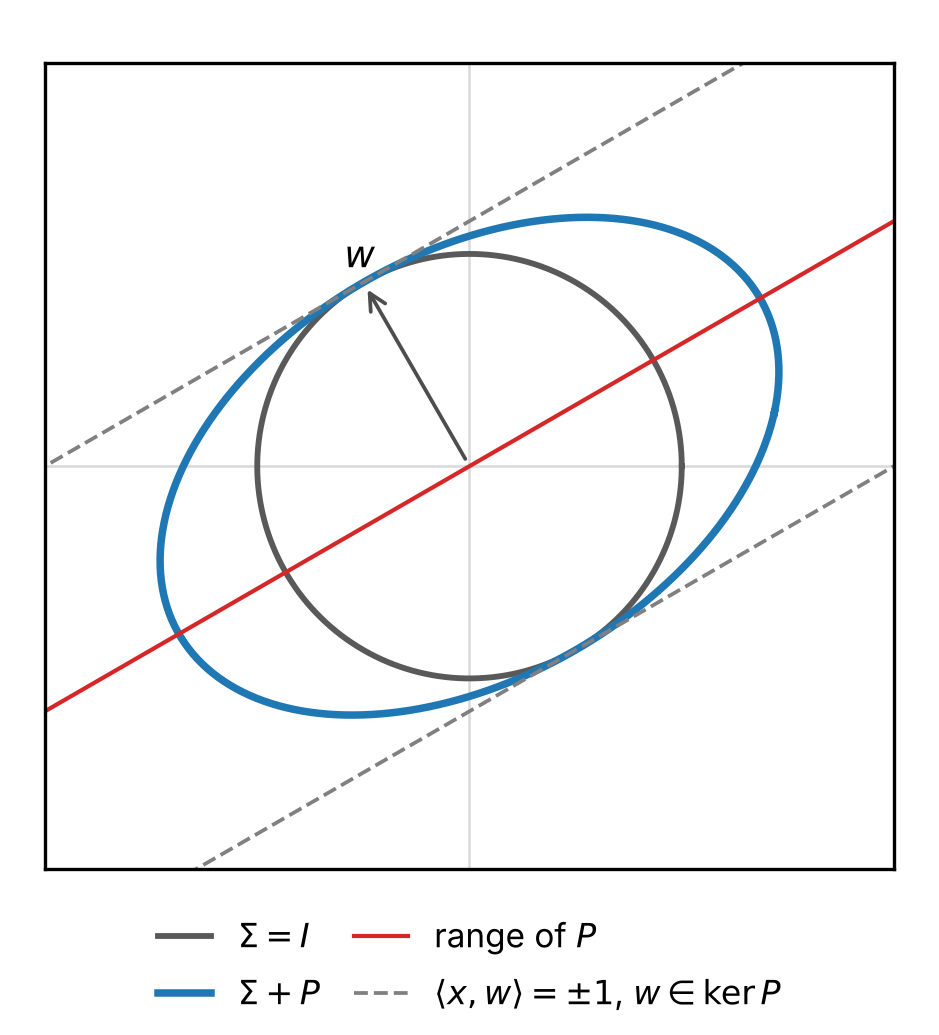
\includegraphics[width=0.5\textwidth]{fig-rank-deficient-step.png}
\caption{A rank-one Loewner step in the plane, from $\Sigma = I$ to $\Sigma + P$ with
$P = \tfrac32\,uu^{\tp}$, $u = (\cos 30^\circ, \sin 30^\circ)$: the apertures $\{x : \langle x, \Sigma^{-1}x\rangle \le 1\}$ of the two
matrices. The aperture widens along the range $\RR u$ of $P$. Its extent in a unit direction $w$ of
% Round 2 (presentation review), item 10: "unit" direction, which the tangent lines need.
the null space $\ker P$, which is $\langle w, \Sigma w\rangle^{1/2}$, is unchanged, so both ellipses touch the
lines $\langle x, w\rangle = \pm 1$. When the kernels depend on $\Sigma$ through one function $g$,
continuous at $0$ with $g(0) = 0$, Theorem~\ref{thm:rank-deficient-step} says that an increment of
such a step that is a probability measure is a centred Gaussian law carried by $\RR u$, the point
mass $\delta_0$ when $g \equiv 0$. Drawn by a script deposited with the paper.}
\label{fig:rank-deficient-step}
\end{figure}

% shared with blueprint thm:affine-rigidity
\begin{theorem}[affine rigidity: the affine Gaussian scale space]\label{thm:affine-rigidity}
Let $d \ge 2$. A family $(\mu_{\Sigma,\Sigma'})$ is an affine cascade family in dimension $d$ if
and only if it is the affine Gaussian scale space with some constant $b > 0$
(\ref{eq:affine-gaussian}). In particular the kernel from scale zero at $I$ of an affine cascade
family in dimension $d \ge 2$ is a centred Gaussian law with covariance a positive multiple of $I$,
and no other probability law on $\RR^d$ is the kernel $\mu_I$ of one.
\end{theorem}

Read against Theorem~\ref{thm:isotropic-classification} and Proposition~\ref{prop:isotropic-corner}(1),
the theorem says that for $d \ge 2$ no isotropic family with a non-Gaussian kernel is, after a change
of gauge, the slice of an affine cascade family, since the kernel $\mu_I$ of an affine cascade family
is Gaussian. The proof turns on the single step.

% shared with blueprint thm:rank-deficient-step
\begin{theorem}[one rank-deficient step forces the Gaussian]\label{thm:rank-deficient-step}
Let $d \ge 2$ and let $g : [0,\infty) \to [0,\infty)$ be continuous at $0$ with $g(0) = 0$.
Suppose there are $\Sigma \in \PD(d)$, $P \in \PSD(d)$ with $0 < \rank P < d$, and a probability
measure $\rho$ on $\RR^d$ with
\begin{equation}\label{eq:one-step}
  e^{-g(\langle\omega,(\Sigma+P)\omega\rangle)}
   = e^{-g(\langle\omega,\Sigma\omega\rangle)}\,\widehat\rho(\omega)
   \qquad (\omega \in \RR^d).
\end{equation}
Then $g(u) = b\,u$ with $b = g(1) \ge 0$, and $\rho$ is the centred Gaussian law with covariance
$2bP$. Conversely, if $g(u) = bu$ with $b \ge 0$, then \ref{eq:one-step} holds with that Gaussian
$\rho$ for every $\Sigma, P \in \PSD(d)$.
\end{theorem}

The hypotheses are about one step alone: $\rho$ is any probability measure, and $g$ is any
nonnegative function continuous at $0$ with $g(0) = 0$, whether or not
$e^{-g(\langle\omega,\Sigma\omega\rangle)}$ is a characteristic function. A step of full rank widens
the aperture in every direction, and $\ker P = \{0\}$ leaves the subspace argument nothing to act
on. Whether such a step can have a probability measure as its increment depends on $g$: for the
\Matern{} orbit no full-rank step can (Proposition~\ref{prop:matern-steps}), and for the isotropic
stable orbit the steps of a cone can (Proposition~\ref{prop:stable-step-cone}).

The proofs of the two theorems rest on three lemmas, proved in Appendix~\ref{app:classical}.

% shared with blueprint lem:charfn-one-on-subspace
\begin{lemma}[a characteristic function equal to $1$ on a subspace]\label{lem:charfn-one-on-subspace}
Let $\rho$ be a probability measure on $\RR^d$ and $H \subseteq \RR^d$ a linear subspace with
$\widehat\rho(\eta) = 1$ for every $\eta$ in a neighbourhood of $0$ in $H$. Then $\rho$ is carried
by the orthogonal complement $H^\perp$, and $\widehat\rho(\omega + \eta) = \widehat\rho(\omega)$ for all
$\omega \in \RR^d$ and $\eta \in H$. In particular, if $\widehat\rho = 1$ near $0$ then
$\rho = \delta_0$.
\end{lemma}

The second statement of the lemma also follows from a general fact. For a positive definite function
$f$ with $f(0) = 1$, the set $G_f$ where $|f| = 1$ is a group, and $f(x + y) = f(x)f(y)$ for
$x \in G_f$ and every $y$ (\sscite{sasvari2013multivariate}, Cor.~1.4.13, p.~29). For $f = \widehat\rho$,
every $\eta \in H$ is a sum of points of the neighbourhood where $\widehat\rho = 1$, so the product rule
gives $\widehat\rho(\eta) = 1$. Then $\widehat\rho(\omega + \eta) = \widehat\rho(\eta)\widehat\rho(\omega) =
\widehat\rho(\omega)$.

The next lemma reduces an affine cascade family to one function of one variable. Covariance makes the kernels from scale zero depend on $\Sigma$ through $\langle\omega,\Sigma\omega\rangle$. Along the ray of $I$ the
cascade (K1) and continuity (K2) exclude a first zero of the transform, so the transform is positive
and $g$ is its negative logarithm. Nondegeneracy (K4) makes $g \not\equiv 0$.

% shared with blueprint lem:affine-reduction
\begin{lemma}[reduction to one function]\label{lem:affine-reduction}
Let $(\mu_{\Sigma,\Sigma'})$ be an affine cascade family in dimension $d$. There is a continuous
$g : [0,\infty) \to [0,\infty)$ with $g(0) = 0$ and $g \not\equiv 0$ such that
\begin{equation}\label{eq:affine-reduction}
  \widehat\mu_\Sigma(\omega) = e^{-g(\langle\omega,\Sigma\omega\rangle)}
  \qquad (\Sigma \in \PSD(d),\ \omega \in \RR^d),
\end{equation}
and for every pair $\Sigma \le \Sigma'$
\begin{equation}\label{eq:affine-increment}
  \widehat\mu_{\Sigma,\Sigma'}(\omega)
   = \exp\bigl[-g(\langle\omega,\Sigma'\omega\rangle) + g(\langle\omega,\Sigma\omega\rangle)\bigr] .
\end{equation}
\end{lemma}

A single Loewner step turns \ref{eq:affine-increment} into a functional equation for $g$, which the next
lemma solves.

% shared with blueprint lem:single-ratio-cauchy
\begin{lemma}[one ratio forces linearity]\label{lem:single-ratio-cauchy}
Let $g : [0,\infty) \to [0,\infty)$ be continuous at $0$ with $g(0) = 0$, and let $a > 1$ be such
that
\begin{equation}\label{eq:single-ratio}
  g(au + w) - g(u + w) = g(au) - g(u) \qquad \text{for all } u > 0,\ w \ge 0 .
\end{equation}
Then $g(u) = b\,u$ for every $u \ge 0$, with $b = g(1) \ge 0$.
\end{lemma}

With the three lemmas the two theorems are proved, the single step first.



% proof of thm:rank-deficient-step
\begin{proof}[Proof of Theorem~\ref{thm:rank-deficient-step}]
\emph{Transport to the identity and diagonalize.} Put $P' := \Sigma^{-1/2}P\Sigma^{-1/2} \in
\PSD(d)$, of rank $r := \rank P$, and choose $Q \in \Orth(d)$ with
$Q^{\tp}P'Q = \diag(p_1,\dots,p_r,0,\dots,0)$, $p_i > 0$. For $\omega = \Sigma^{-1/2}Q\zeta$ one
has $\langle\omega,\Sigma\omega\rangle = |\zeta|^2$ and
$\langle\omega,P\omega\rangle = \sum_{i \le r}p_i\zeta_i^2$. Let $C := Q^{\tp}\Sigma^{-1/2}$ and
$\rho' := C_*\rho$, so that $\widehat{\rho'}(\zeta) = \widehat\rho(C^{\tp}\zeta)
= \widehat\rho(\Sigma^{-1/2}Q\zeta)$. Dividing \ref{eq:one-step} by
$e^{-g(\langle\omega,\Sigma\omega\rangle)}$, which has no zero,
\[
  \widehat{\rho'}(\zeta) = \exp\Bigl[-g\Bigl(|\zeta|^2 + \sum_{i\le r}p_i\zeta_i^2\Bigr)
     + g\bigl(|\zeta|^2\bigr)\Bigr] .
\]

\emph{The subspace.} On $H := \{\zeta : \zeta_1 = \dots = \zeta_r = 0\}$, of dimension
$d - r \ge 1$, the exponent vanishes and $\widehat{\rho'} = 1$. By
Lemma~\ref{lem:charfn-one-on-subspace}, $\widehat{\rho'}(\zeta + \eta) = \widehat{\rho'}(\zeta)$ for
$\eta \in H$. Take $\zeta = t e_1$ with $t > 0$ and $\eta \in H$ arbitrary, and put
$a := 1 + p_1 > 1$, $u := t^2$, $w := |\eta|^2$: the invariance reads
\[
  g(au + w) - g(u + w) = g(au) - g(u) ,
\]
and as $t$ ranges over $(0,\infty)$ and $\eta$ over $H \ne \{0\}$, the pair $(u,w)$ ranges over
$(0,\infty) \times [0,\infty)$. That is \ref{eq:single-ratio}, and
Lemma~\ref{lem:single-ratio-cauchy} gives $g(u) = bu$ with $b = g(1) \ge 0$.

\emph{The increment, and the converse.} Now \ref{eq:one-step} reads
$\widehat\rho(\omega) = e^{-b\langle\omega,P\omega\rangle}$, the characteristic function of the
centred Gaussian law with covariance $2bP$ (the law of $(2bP)^{1/2}Z$, $Z$ standard normal on
$\RR^d$); by uniqueness of the transform $\rho$ is that law. Conversely, for $g(u) = bu$ the
exponents in \ref{eq:one-step} are linear in the matrix, and the same Gaussian satisfies it for any
$\Sigma, P \in \PSD(d)$.
\end{proof}

% proof of thm:affine-rigidity
\begin{proof}[Proof of Theorem~\ref{thm:affine-rigidity}]
\emph{Necessity.} By Lemma~\ref{lem:affine-reduction} there is a continuous $g \ge 0$ with $g(0) = 0$
and $g \not\equiv 0$ satisfying \ref{eq:affine-reduction} and \ref{eq:affine-increment}. Take
$\Sigma = I$ and $P = e_1e_1^{\tp}$, of rank $1 < d$, and $\rho := \mu_{I,I+P}$, a probability
measure. Then \ref{eq:affine-increment} at the pair $I \le I + P$, multiplied by
$e^{-g(|\omega|^2)}$, is \ref{eq:one-step}. So Theorem~\ref{thm:rank-deficient-step} gives $g(u) = bu$,
and $b > 0$ because $g \not\equiv 0$. Now \ref{eq:affine-increment} is \ref{eq:affine-gaussian} for
every pair, and by uniqueness of the transform each $\mu_{\Sigma,\Sigma'}$ is the stated Gaussian.

\emph{Sufficiency.} Let $b > 0$ and let $\mu_{\Sigma,\Sigma'}$ be the centred Gaussian with
covariance $2b(\Sigma'-\Sigma)$, which exists for every positive semidefinite covariance as the law
of $(2b(\Sigma'-\Sigma))^{1/2}Z$. Its transform is \ref{eq:affine-gaussian}. The axioms of
Definition~\ref{def:affine-cascade-family} hold. (K1): the transform
at $\Sigma = \Sigma'$ is $1$, and the exponents of $\mu_{\Sigma',\Sigma''}$ and
$\mu_{\Sigma,\Sigma'}$ add to that of $\mu_{\Sigma,\Sigma''}$; by uniqueness of the transform,
$\mu_{\Sigma,\Sigma} = \delta_0$ and the convolution identity holds. (K2): the transform is
continuous in $(\Sigma,\Sigma')$. (K3): $\widehat{A_*\mu_{\Sigma,\Sigma'}}(\omega)
= e^{-b\langle A^{\tp}\omega,(\Sigma'-\Sigma)A^{\tp}\omega\rangle}
= e^{-b\langle\omega,(A\Sigma'A^{\tp} - A\Sigma A^{\tp})\omega\rangle}$. (K4):
$\widehat\mu_{0,I}(e_1) = e^{-b} \ne 1$.

\emph{The last clause.} By necessity, $\widehat\mu_I(\omega) = e^{-b|\omega|^2}$ with $b > 0$.
\end{proof}

The proof uses (K1)--(K4) through Lemma~\ref{lem:affine-reduction} and then one step of the
cascade, $I \le I + e_1e_1^{\tp}$, and of $g$ it needs only continuity at $0$ and $g \ge 0$.

% Round 3 (report B, part 3 (ii); the author's decision D12, PLAN-review-response-paper.md R3.0):
% where continuity enters the rigidity, with the family that shows it is needed there.
Continuity (K2) enters that proof in Lemma~\ref{lem:affine-reduction}, twice: to exclude a first zero of
the transform along the ray of $I$, and to reach the kernels at the singular apertures. The cascade and
the dilations do the first without it, by making $\mu_I$ self-decomposable, and the second cannot be
done without it.

% shared with blueprint prop:affine-rigidity-boundary
\begin{proposition}[continuity is needed only at the boundary of $\PSD(d)$]\label{prop:affine-rigidity-boundary}
Let $d \ge 2$, and let $(\mu_{\Sigma,\Sigma'})$ be probability measures on $\RR^d$, indexed by the pairs
$\Sigma \le \Sigma'$ in $\PSD(d)$, that satisfy (K1), (K3) and (K4) of Definition~\ref{def:affine-cascade-family}, but
not necessarily (K2).
\begin{enumerate}
\item \emph{(Between positive definite apertures.)} There is $b > 0$ such that for every $\Sigma \in \PD(d)$
the kernel from scale zero $\mu_\Sigma$ is the centred Gaussian law with covariance $2b\Sigma$, and for every
pair $\Sigma \le \Sigma'$ in $\PD(d)$ the increment $\mu_{\Sigma,\Sigma'}$ is the centred Gaussian law with
covariance $2b(\Sigma' - \Sigma)$. In particular $\mu_I$ is the centred Gaussian law with covariance $2bI$.
\item \emph{(At the boundary.)} Let $b > 0$ and $0 \le \theta_0 < 1$, put $\theta(\Sigma) := 1$ for
$\Sigma \in \PD(d)$ and $\theta(\Sigma) := \theta_0$ for singular $\Sigma \in \PSD(d)$, and for
$\Sigma \le \Sigma'$ let $\mu_{\Sigma,\Sigma'}$ be the centred Gaussian law with covariance
$2b(\theta(\Sigma')\Sigma' - \theta(\Sigma)\Sigma)$. This covariance is positive semidefinite for every pair,
and the family satisfies (K1), (K3) and (K4) and agrees with the affine Gaussian scale space with constant
$b$ on the pairs in $\PD(d)$. Its kernel from scale zero at a nonzero singular $P$ has covariance
$2b\theta_0P$, so the family is not an affine Gaussian scale space, and it does not satisfy (K2).
\end{enumerate}
\end{proposition}

\begin{proof}
\emph{(1).} Let $\vartheta(u) := \widehat\mu_I(\sqrt u\,e_1)$, $u \ge 0$. As in the first step of the proof of
Lemma~\ref{lem:affine-reduction}, which reads only (K3), $\mu_I$ is rotation invariant,
$\widehat\mu_I(\omega) = \vartheta(|\omega|^2)$, and $\vartheta$ is continuous and real with $\vartheta(0) = 1$
and $|\vartheta| \le 1$. For $\Sigma \in \PD(d)$, (K3) with $A = \Sigma^{1/2}$ gives
$\widehat\mu_\Sigma(\omega) = \vartheta(\langle\omega,\Sigma\omega\rangle)$. For $0 < c < 1$, (K1) at
$0 \le c^2I \le I$ gives $\mu_I = \mu_{c^2I} * \mu_{c^2I,I}$, and (K3) with $A = cI$ at the pair $(0, I)$
gives $\mu_{c^2I} = (cI)_*\mu_I$. So $\mu_I$ is self-decomposable \ref{eq:self-decomposable}, and its
transform has no zero (Proposition~\ref{prop:gw-ray-families}(1)). Being real and continuous with $\vartheta(0) = 1$,
$\vartheta$ is then positive, and $g := -\log\vartheta$ is continuous, nonnegative and $g(0) = 0$. If
$g \equiv 0$, then $\widehat\mu_I \equiv 1$ and $\mu_I = \delta_0$ (Lemma~\ref{lem:charfn-one-on-subspace}), against
(K4). Put $P := e_1e_1^{\tp}$, of rank $1 < d$. (K1) at $0 \le I \le I + P$ gives
$\mu_{I+P} = \mu_{I,I+P} * \mu_I$, which is \ref{eq:one-step} with $\Sigma = I$ and $\rho = \mu_{I,I+P}$. So
Theorem~\ref{thm:rank-deficient-step} gives $g(u) = bu$ with $b = g(1)$, and $b > 0$ as $g \not\equiv 0$. Hence
$\widehat\mu_\Sigma(\omega) = e^{-b\langle\omega,\Sigma\omega\rangle}$ for $\Sigma \in \PD(d)$, the transform of
the centred Gaussian law with covariance $2b\Sigma$. For $\Sigma \le \Sigma'$ in $\PD(d)$, (K1) at
$0 \le \Sigma \le \Sigma'$ gives $\widehat\mu_{\Sigma'} = \widehat\mu_{\Sigma,\Sigma'}\,\widehat\mu_\Sigma$, and as
$\widehat\mu_\Sigma$ has no zero, $\widehat\mu_{\Sigma,\Sigma'}(\omega) = e^{-b\langle\omega,(\Sigma'-\Sigma)\omega\rangle}$.
The uniqueness of the transform names each law.

\emph{(2), the covariances.} Let $\Sigma \le \Sigma'$ and $D := \theta(\Sigma')\Sigma' - \theta(\Sigma)\Sigma$. If
$\Sigma$ is definite, so is $\Sigma' \ge \Sigma$, and $D = \Sigma' - \Sigma \ge 0$. If both are singular,
$D = \theta_0(\Sigma' - \Sigma) \ge 0$. If $\Sigma$ is singular and $\Sigma'$ definite,
$D = \Sigma' - \theta_0\Sigma = (\Sigma' - \Sigma) + (1 - \theta_0)\Sigma \ge 0$. So each $\mu_{\Sigma,\Sigma'}$ exists,
with transform $e^{-b\langle\omega,D\omega\rangle}$.

\emph{(2), the axioms.} (K1): at $\Sigma = \Sigma'$, $D = 0$. For $\Sigma \le \Sigma' \le \Sigma''$ the
matrices $D$ of the pairs $(\Sigma, \Sigma')$ and $(\Sigma', \Sigma'')$ add to that of $(\Sigma, \Sigma'')$, so the
transforms multiply and the uniqueness of the transform gives the cascade identity. (K3): an $A \in \GL(d)$
preserves rank, so $\theta(A\Sigma A^{\tp}) = \theta(\Sigma)$, and $A_*\mu_{\Sigma,\Sigma'}$, the centred Gaussian
law with covariance $2bADA^{\tp}$, is $\mu_{A\Sigma A^{\tp},\,A\Sigma'A^{\tp}}$. (K4): $\theta(0)\,0 = 0$, so
$\mu_{0,I}$ has covariance $2bI$ and is not $\delta_0$. On a pair in $\PD(d)$, $D = \Sigma' - \Sigma$, which is
\ref{eq:affine-gaussian}. For a nonzero singular $P$, $\mu_{0,P}$ has covariance $2b\theta_0P$. An affine Gaussian scale space
with this $\mu_{0,I}$ has the constant $b$, by \ref{eq:affine-gaussian} at the pair $(0, I)$, and its kernel at $P$
has covariance $2bP \ne 2b\theta_0P$, as $\theta_0 < 1$ and $P \ne 0$. Finally, $P + n^{-1}I$ is
definite and tends to $P$, while for $\omega$ with $P\omega \ne 0$,
$\widehat\mu_{0,P+n^{-1}I}(\omega) = e^{-b\langle\omega,(P+n^{-1}I)\omega\rangle} \to e^{-b\langle\omega,P\omega\rangle}
\ne e^{-b\theta_0\langle\omega,P\omega\rangle} = \widehat\mu_{0,P}(\omega)$. So (K2) fails at the pair $(0, P)$.
\end{proof}

So by Proposition~\ref{prop:affine-rigidity-boundary}, on the positive definite apertures the axioms need no
continuity, and Iijima's, as reported in
Remark~\ref{rem:lindeberg}, list none. Continuity fixes only the kernels and increments at the singular
apertures.

\begin{remark}[positivity carries weight]\label{rem:positivity}
The classification theorems of this paper use positivity: their kernels and increments are probability
measures. In the rigidity it enters twice: through
Lemma~\ref{lem:charfn-one-on-subspace}, which says that a probability measure whose transform is $1$ on a
subspace is carried by its orthogonal complement, and through the sign of the function $g$ of
Lemma~\ref{lem:affine-reduction}. That function is nonnegative because the transform of a probability
law has modulus at most $1$, and Lemma~\ref{lem:single-ratio-cauchy} uses the sign, with continuity at
$0$, in place of every other regularity in Cauchy's equation. Without
positivity the increments need not be signed measures: across shapes the increment of the \Matern{} orbit of
index $1$ is not even a finite signed measure (Proposition~\ref{prop:matern-negative-mass}(3)).
\end{remark}

The theorem holds on operators too. The passage from operators to kernels
(Lemma~\ref{lem:operators-to-kernels}) has a converse, from a family of kernels to a
family of operators continuous in $L^1$ (Lemma~\ref{lem:kernels-to-operators}, both in
Appendix~\ref{app:classical}), and the two together carry the rigidity over.

% shared with blueprint thm:affine-rigidity-operators+3a6bc0ff67da
\begin{theorem}[affine rigidity on operators]\label{thm:affine-rigidity-operators}
Let $d \ge 2$. A family $(\Phi_{\Sigma,\Sigma'})$ of linear operators on $L^1(\RR^d)$, indexed by the
pairs $\Sigma \le \Sigma'$ in $\PSD(d)$, is a $(\GL(d), \text{Loewner})$-cascade family of operators
(Definition~\ref{def:gw-cascade-family}(1)) if and only if there is $b > 0$ such that
$\Phi_{\Sigma,\Sigma'}f = \mu_{\Sigma,\Sigma'} * f$ for every pair and every $f \in L^1(\RR^d)$, where
$(\mu_{\Sigma,\Sigma'})$ is the affine Gaussian scale space with constant $b$
(Definition~\ref{def:affine-cascade-family}, \ref{eq:affine-gaussian}). The constant $b$ is then unique.
\end{theorem}

\begin{proof}
\emph{Necessity.} By Lemma~\ref{lem:operators-to-kernels}(4) the measures $\mu_{\Sigma,\Sigma'}$
with $\Phi_{\Sigma,\Sigma'}f = \mu_{\Sigma,\Sigma'} * f$ form an affine cascade family in dimension
$d$, and by Theorem~\ref{thm:affine-rigidity} it is the affine Gaussian scale space with some $b > 0$.

\emph{Sufficiency.} By Theorem~\ref{thm:affine-rigidity} the affine Gaussian scale space with constant
$b > 0$ is an affine cascade family, that is a $(\GL(d), \text{Loewner})$-cascade family of kernels,
and $(\GL(d), \text{Loewner})$ is a wedge datum (Definition~\ref{def:gw-cascade-family}). By
Lemma~\ref{lem:kernels-to-operators}(2) the operators $f \mapsto \mu_{\Sigma,\Sigma'} * f$ form a
$(\GL(d), \text{Loewner})$-cascade family of operators.

\emph{Uniqueness of $b$.} If $\Phi_{0,I}$ is convolution by the Gaussian laws of constants $b$ and
$b'$, the uniqueness clause of Lemma~\ref{lem:operators-to-kernels}(1) makes the two laws equal, and their
transforms \ref{eq:affine-gaussian} at $\Sigma = 0$, $\Sigma' = I$ and $\omega = e_1$ give
$e^{-b} = e^{-b'}$.
\end{proof}

\subsection{Prior art, and the relation to the line}\label{sec:classical-prior-art}

This subsection places Theorem~\ref{thm:affine-rigidity} among the axiomatics of scale space and the
characterizations of the normal law. The family it selects is classical, and so is its covariance
under linear maps. The morphological axiomatics reads ``affine'' in another sense, and the
$\alpha$-scale spaces admit the stable laws, which the classical corner removes. As a
characterization of the normal law its core is Kelker's lemma (Remark~\ref{rem:kelker}), and as an
axiomatic derivation it stands beside Lindeberg's (Remark~\ref{rem:lindeberg}).
Remark~\ref{rem:classical-line} reads the scheme on the line.

The affine Gaussian scale space is classical. Lindeberg and G\aa{}rding define it in the plane by
the Gaussian kernels of the positive semidefinite covariance matrices, and it is closed under linear changes of
the image coordinates: an invertible $B$ moves the matrix by $\Sigma \mapsto B\Sigma B^{\tp}$
% Round 3 (content review), A.R10: p. 10 and the equation numbers are the KTH report's, not the
% journal article's; the held copy is the report. Both are dropped, and the next sentence's "the same
% page" (report p. 10, section 4.1, read again for this edit) becomes the section.
(\sscite{lindeberg1997shape}, \S\S4 and~4.1). The rotationally symmetric
linear scale space has that closure only for rotations and uniform rescalings (the same source, \S4.1).

The word ``affine'' has another sense in the morphological axiomatics of Alvarez, Guichard, Lions
and Morel. There the scale stays a scalar $t$, and a linear map $A$ of the image is required to be
absorbed by a change of that scalar, $AT_{t'} = T_tA$ for some $t'(t, A)$
(\sscite{alvarez1993axioms}, [Projection invariance], p.~206). In the plane, with grey-scale and
scale invariance among the hypotheses, this leaves the nonlinear affine morphological scale space
$\partial u/\partial t = |Du|\,(t\operatorname{curv}(u))^{1/3}$ (Thm.~5(iii), p.~229). Their
linear multiscale analyses with isometric invariance are the heat equation, up to a rescaling of
$t$ (Thm.~3, p.~214), and its rotationally symmetric kernels are not closed under an anisotropic
map. Indexing the kernels by matrices is what lets a linear, positive family be covariant under
$\GL(d)$. With the cascade along the whole Loewner order and $d \ge 2$,
Theorem~\ref{thm:affine-rigidity} says that the Gaussian is then the only one.

The other neighbours are the axiomatics that admit the stable laws. For linear, even, recursive
and scale-invariant filters on the line, Pauwels, Van Gool, Fiddelaers and Moons obtain the
transforms $e^{-a|\omega|^\alpha t}$, $\alpha > 0$, so that these conditions do not single out the
Gaussian (\sscite{pauwels1995extended}, p.~694). The kernels have zero crossings for $\alpha > 2$
(pp.~694--695). Duits, Florack, de Graaf and ter Haar Romeny write this class on $\RR^d$ as the
$\alpha$ scale spaces generated by $-(-\Delta)^\alpha$ (\sscite{duits2004axioms}, (25), p.~277),
whose transforms are $e^{-s|\omega|^{2\alpha}}$. Under positivity the parameter lies in $(0, 1]$,
with $\alpha = \tfrac12$ the Poisson and $\alpha = 1$ the Gaussian scale space (p.~267). Pauwels'
$\alpha$ is the stable index of this paper, and the $\alpha$ of Duits et al.\ is half of it. Where they
are positive, the kernels of both classes are the isotropic stable laws, which the isotropic theory contains. For $d \ge 2$ the classical corner removes them: by Theorem~\ref{thm:affine-rigidity} no stable law other than the Gaussian is the
kernel $\mu_I$ of an affine cascade family. Felsberg and Sommer show that the planar Poisson kernel
satisfies Iijima's axioms for a scalar scale (\sscite{felsberg2004monogenic}, Thm.~1, p.~7), and in an
earlier outlook propose a $2 \times 2$ scaling matrix in place of that scale
(\sscite{felsberg2001scale}, \S5, p.~130). The elliptical Poisson orbit is the stable orbit of
index~$1$, whose positive increments form the cone of Proposition~\ref{prop:stable-step-cone}(1), with
no rank-deficient step in it (Theorem~\ref{thm:rank-deficient-step}).

Two earlier results bear on Theorem~\ref{thm:affine-rigidity} directly: Kelker's characterization of
the normal law, which is its core (Remark~\ref{rem:kelker}), and Lindeberg's derivation of the same
family from other axioms (Remark~\ref{rem:lindeberg}).

\begin{remark}[Kelker's lemma]\label{rem:kelker}
A rotation-invariant law with independent coordinates is normal. In the plane this is the
Herschel--Maxwell theorem (\sscite{bryc1995normal}, Thm.~0.0.1, p.~1).
% Bryc read at the page (Q-0294; records/affine/READING-bryc1995normal.md).
In every dimension it is Kelker's lemma, proved for the centred laws whose transform has the form
$\psi(\langle\omega,\Sigma\omega\rangle)$ with $\Sigma$ diagonal, of which the rotation-invariant
laws are the case $\Sigma = I$ (\sscite{kelker1970distribution}, Lemma~5, p.~423). Fang, Kotz and Ng restate it with pairwise independence
(\sscite{fang1990symmetric}, Thm.~4.11, p.~106). The following sketch shows that it is the core of
Theorem~\ref{thm:affine-rigidity}. From the base $I - e_1e_1^{\tp}$ of an affine cascade family,
$\mu_I = \mu_{I - e_1e_1^{\tp}} * \mu_{I - e_1e_1^{\tp},\,I}$, and by
Lemma~\ref{lem:charfn-one-on-subspace} the first factor is carried by $e_1^\perp$ and the second by
the $e_1$-axis. So the first coordinate of $\mu_I$ is independent of the others.
% Round 3 (content review), B.S6: the step to mutual independence, and where the base lies.
By rotation invariance every coordinate is, so the transform factors over the coordinates. The
coordinates are then independent, and Kelker's lemma makes $\mu_I$ normal. The step used has a singular base, which lies
outside Theorem~\ref{thm:rank-deficient-step} and inside Definition~\ref{def:affine-cascade-family}. What the scale-space
setting adds is the single-step form, Theorem~\ref{thm:rank-deficient-step}. It reads one step
$\Sigma \to \Sigma + P$, with $\Sigma$ positive definite and $P$ singular, whose increment is any
probability measure. And $e^{-g(\langle\omega,\Sigma\omega\rangle)}$ need not be a characteristic
function there. Kelker, Fang, Kotz and Ng, Bryc,
and Cambanis, Huang and Simons characterize the normal law among the \emph{elliptically contoured}
laws, the linear images of rotation-invariant laws shifted by a vector, by
properties of one vector, such as independent coordinates, conditional laws, quadratic forms or
marginal densities (\sscite{kelker1970distribution}, Lemma~5, p.~423, Thm.~7 and Lemma~8,
pp.~424--426; \sscite{cambanis1981theory}, \S5, pp.~379--384). Khatri and Mukerjee characterize the
normal law by the law of one quadratic form, and Anderson and Fang by the independence of two complementary
quadratic forms of one spherical vector (\sscite{khatri1987characterization}, Thm.~1, p.~187;
\sscite{anderson1987cochran}, Thm.~1, p.~309). Kelker's route, and that of Cambanis, Huang and
Simons, goes through Cauchy's equation for the generator, as Lemma~\ref{lem:single-ratio-cauchy} does
(\sscite{kelker1970distribution}, p.~423; \sscite{cambanis1981theory}, Thm.~6, pp.~379--380).
% Q-0314: Khatri-Mukerjee and Anderson-Fang read at the page (READING-khatri1987characterization.md,
% READING-anderson1987cochran.md): one-vector characterizations, by moment series and through
% Lukacs's gamma characterization; the TODO(source) is closed, and the claim stays "not found in the
% sources read". The earlier text had lost the subject of the Cauchy sentence inside that comment.
% Writing-rules follow-up (2026-10-14; PASS-writing-rules-affine.md, owed item 3): that claim, and
% "None of these sources relates two scale matrices of one generator by a convolution", are gone
% (the author's direction against novelty claims); the contrast stays in "by properties of one vector".
% Q-0317 (the blind register review, section 3 flag 13): the subject of the next sentence had been
% swallowed into this comment's last line; it is restored on its own line.
Where the Gaussian has the whole Loewner order, the non-Gaussian orbits keep cones of full-rank steps
(Propositions~\ref{prop:stable-step-cone} and~\ref{prop:orbit-step-cone}).
% Q-0309 (fix group 5): Cambanis-Huang-Simons read at the page by Q-0308
% (records/affine/READING-cambanis1981theory.md): non-proportional scale matrices occur there only as
% non-uniqueness (Thm. 3(i), pp. 372-373); no statement on sums or convolutions of elliptical
% vectors. Fang-Kotz-Ng 4.3 (READING-fang1990symmetric.md) and Bryc (READING-bryc1995normal.md) as
% before. The review's lead (flag 46) is not in these sources; PRIOR-ART-novelty-claims.md lists
% what a referee could still name (Anderson-Fang, Khatri-Mukerjee; Kelker pp. 424-430).
% Q-0312: Kelker pp. 424-430 read on the images (READING-kelker1970distribution.md, section 5):
% regression, conditional covariance (Thm. 7), conditional normality (Lemma 8), Schoenberg, norms
% and quadratic forms, all of one vector; nothing relates two scale matrices by a convolution.
A form without any
covariance group, with the Darmois--Skitovich theorem (\sscite{skitovich1954linear}, Thm.~2,
p.~190) in place of Kelker's lemma, is open
problem~\ref{prob:no-covariance} of \S\ref{sec:open-problems}.
\end{remark}

\begin{remark}[Lindeberg's and Iijima's derivations]\label{rem:lindeberg}
Lindeberg \sscite{lindeberg2011generalized} assumes a semigroup in a scalar scale $s$, strong
continuity with a Sobolev regularity condition, and non-enhancement of local extrema. From these,
his Theorem~5 (p.~42) obtains a local generator of order two with a positive semidefinite matrix
$\Sigma_0$, and the affine Gaussian scale space is its positive definite, mirror-symmetric case
(\S4.1.2, p.~45). Positivity, unit mass and closure under affine maps are properties of his
solution, not axioms, and non-enhancement is what removes the stable laws (\S2, p.~39).
Theorem~\ref{thm:affine-rigidity} takes as axioms positivity, a cascade over Loewner-ordered pairs
of matrices, continuity in the pair, nondegeneracy at one pair and $\GL(d)$-covariance, for $d \ge 2$.
The two results have different shapes. His classifies all non-enhancing continuous semigroups, one
Gaussian ray $\{s\Sigma_0\}$ for each matrix $\Sigma_0$ and drift, with the affine group acting on
the rays afterwards. This one is a rigidity statement for one two-parameter family with a group
action. Neither implies the other from its own hypotheses: his axioms have no positivity and no
order on matrices, and this one has no non-enhancement and does not cover $d = 1$. The order appears
in his later work as the meaning of a larger matrix scale (\sscite{lindeberg2013computational}, fn.~7,
p.~594). On the ray from
$\Sigma = 0$ to $\Sigma' = s\Sigma_0$, the kernel of \ref{eq:affine-gaussian} with $b = \tfrac12$ is
his kernel (45), p.~44, with zero drift.

Iijima's axioms of 1962 and 1963, as Weickert, Ishikawa and Imiya report them
(\sscite{weickert1999linear}, p.~241), are closer in form. The scale is a positive definite
$2 \times 2$ matrix. The transformations are linear, translation invariant and positive, and they are
closed under every invertible linear map. Any two of them compose to a third member of the family,
with no order on the scales. These axioms give the affine Gaussian scale space. For a scalar scale,
Felsberg and Sommer find that Iijima's uniqueness proof assumes implicitly a transform continuously
differentiable at the origin, which that of the Poisson kernel is not (\sscite{felsberg2004monogenic},
p.~8, and n.~2, p.~24). As hypotheses the two
sets are incomparable. Iijima composes every pair of scales and asks that the composite be in the
family. Theorem~\ref{thm:affine-rigidity} indexes its increments by pairs, does not ask that they be
members, and asks for them only from a matrix to a larger one in the Loewner order.
% Round 3 (content review), B.S2 (the author's decision D12): the pointer to Proposition 3.11.
It adds continuity in the pair, which is needed only at the singular matrices
(Proposition~\ref{prop:affine-rigidity-boundary}). It holds for every $d \ge 2$.
\end{remark}

\begin{remark}[relation to the line]\label{rem:classical-line}
At $d = 1$, $\PSD(1) = [0,\infty)$, and the Loewner order and the ray order are both the order of
the half-line. The similarities are all of $\GL(1)$, so the four corners of
Definition~\ref{def:gw-cascade-family} coincide, and every pair is on the slice. By
Proposition~\ref{prop:isotropic-corner}(1) and (2) with $d = 1$, the families of the scheme are then
the isotropic families in dimension $1$, read in the variance gauge, and those are the line's
families of Definition~\ref{def:line-family} on kernels \prog{Iso}{Rem.~3.26}.
So on the
line the classical corner is the line's theory with its gauge fixed, and the kernel $\mu_1$ at
scale $1$ of such a family can be any symmetric self-decomposable law other than $\delta_0$, and
only such a law (Theorem~\ref{thm:line-classification}). On the line the relabelling of the scales
is free, and the gauge $\chi$ of Theorem~\ref{thm:line-classification} is part of the answer. For $d \ge 2$ and
$G = \GL(d)$ the group acts transitively on $\PD(d)$, and Lemma~\ref{lem:affine-gauge} forces the
parametrization up to one constant. The rigidity belongs to dimension $d \ge 2$:
Theorem~\ref{thm:rank-deficient-step} needs a step with $0 < \rank P < d$, which the line does not
have.
\end{remark}

% §5 The affine landscape --- blueprint chapter 5 (blueprint/src/parts/05-*.tex). Written from the
% draft's §5 (Q-0288, 2026-10-04) on the template of sections 2 and 3 (spatial-hemigroup-affine #43).
% Every statement is transcribed verbatim from its node under a `% shared with blueprint` marker,
% with the paper statement's \label equal to the blueprint label (records/affine/
% transcribe-shared-statements.py), so that `linkage check` reports it `verbatim`. The drafting gate
% is records/affine/GATE-section-5.md.
%
% Files. The section is long, so it is split into parts: this file (the opening, 5.1 and 5.2),
% 05-table.tex (5.3, the overview table and the statement of thm:wedge-axis), 05-wedges.tex (5.4),
% 05-orbits.tex (5.5, 5.6), 05-smaller-groups.tex (5.7), 05-wedge-axis.tex (5.8, the proof of
% thm:wedge-axis) and 05-shape-adapted.tex (5.9, with the section's relation remark).
%
% Order (Q-0290, after the blind review records/affine/REVIEW-paper-section-5.md). The blueprint's,
% which follows the plan (notes/PLAN-article-structure.md, "§5"), with two changes: the overview
% table and the statement of thm:wedge-axis come right after 5.2, as the section's destination, with
% forward references (flag S4), the proof staying after every node it reads (5.8); and
% prop:stable-order-generated sits in 5.6 after prop:stable-exponent-cone, whose cone it reads (flag
% S12). 5.2 names the orbit sets of the smaller groups, proved in 5.7.
%
% Figure (Q-0290, review flag V1): fig-shape-plane.png in 5.2, from records/affine/fig-shape-plane.py
% with its output saved (fig-shape-plane-output.txt); no statement uses it.
%
% Appendices (Q-0290, the author's decision of 2026-10-04 to shorten by moving material, never
% deleting a statement): appendix-orders.tex (A), appendix-matern-cross-shape.tex (B),
% appendix-linear-flow.tex (C), appendix-similarity-loewner.tex (D), appendix-proofs.tex (E). A
% statement moved there goes whole, with its marker; the main text keeps a sentence naming it. A
% proof moved there leaves its statement here, followed by a pointer.
%
% Proofs. The proofs of record are the blueprint's. Short ones are transcribed; long ones are
% shortened to their decisive steps and headed "Sketch", which section 1.1 explains (the full proofs
% are in the deposited blueprint sources). Each proof cites the statements its node uses. The cited
% facts of section 2.6 an [A] node rests on are named, by number and \ref, before the node or, where
% a subsection has several such nodes on the same fact, once at the subsection's start (5.6, 5.7).
%
% Section 4 is written in parallel (Q-0287); its labels (def:gw-cascade-family,
% def:affine-cascade-family, eq:affine-gaussian, lem:operators-to-kernels, lem:affine-gauge,
% lem:parameter-space, thm:cascade-infinitely-divisible, lem:charfn-one-on-subspace,
% lem:single-ratio-cauchy, thm:rank-deficient-step, eq:one-step, thm:affine-rigidity) resolve once
% both sections are merged. Sections 5.1 and 5.8 take their reading of shape-adapted smoothing from
% lindeberg1994shape and lindeberg1997shape, read at the page (records/affine/READING-*.md; the
% stored copy of the 1997 article is the authors' report version, so it is cited by section only).
% The hub's experiments with a stable replacement are not used (the author, 2026-10-04).

\section{The affine landscape}\label{sec:landscape}

Theorem~\ref{thm:affine-rigidity} closes the classical corner of the axiom scheme: for $d \ge 2$, a
family covariant under the whole general linear group that cascades along every step of the Loewner order is an affine
Gaussian scale space. A user who wants another kernel at elliptical apertures, the Poisson kernel or a
\Matern{} kernel, has to give something up, and there are two things to give up. One is covariance, a
smaller group of linear maps of the image. The other is the cascade, an order smaller than the Loewner
order: fewer pairs of apertures $\Sigma, \Sigma'$ along which the record at $\Sigma'$ is a further
smoothing of the record at $\Sigma$. This section maps the families for each choice of the two
(Table~\ref{tab:landscape}). Every order used here is invariant under all of $\GL(d)$, so it pairs
with every group. Along the general linear row the families run from the affine orbits of all
rotation-invariant self-decomposable laws, each a round kernel stretched to every elliptical aperture,
on the rays (Proposition~\ref{prop:ray-families}), to the Gaussian alone, on the Loewner order. In
between, the orbit of the isotropic $\gamma$-stable law, $0 < \gamma < 2$, is a family along the
stable order of index $\alpha$ exactly when $\gamma \ge \alpha$ (Theorem~\ref{thm:wedge-axis}(3)), and
a \Matern{} orbit cascades along the rays and along no other step
(Proposition~\ref{prop:matern-steps}). What turns on the order is how fast an adapted aperture may
change its shape between two scales while the record stays a further smoothing
(\S\ref{sec:landscape-uses}). A smaller group admits more families in every column.

\S\ref{sec:landscape-uses} says what an affine scale space is used for, and what each
use asks of the axioms. \S\ref{sec:scale-shape} lists the groups and reads the Loewner order in volume
and shape. \S\ref{sec:landscape-table} gives the destination first: the overview table of the
families of each group along each order, with forward references. The rest fills it in. \S\ref{sec:invariant-wedges}
describes the invariant orders on positive definite matrices through their cones, which index the
chain of orders along which the general linear row is read. \S\ref{sec:affine-orbits} treats the base of the general linear row, the rays, and
\S\ref{sec:affine-stable-cone} the steps each orbit survives beyond them, up to the stable order on
$\PSD(d)$. \S\ref{sec:wedge-axis-proof} states and proves the theorem on the general linear row.
\S\ref{sec:shape-adapted} reads the practice of shape-adapted smoothing against the families, and
\S\ref{sec:smaller-groups} summarizes the rows of the smaller groups.
Appendices~\ref{app:classical}--\ref{app:wedge-axis} hold the proofs that \S\ref{sec:classical} and
this section defer, Appendix~\ref{app:wedge-axis} the complete proof of the theorem on the general
linear row. Appendices~\ref{app:orientation}--\ref{app:similarity} hold further results that the table
cites.

\subsection{What an affine scale space is for}\label{sec:landscape-uses}

The use of an affine scale space considered here is shape adaptation. An aperture whose shape
fits the local image structure measures the same thing in every affine image of a pattern. The
standard form of this is the iteration of Lindeberg and G\aa{}rding \sscite{lindeberg1994shape}. An
uncommitted, rotationally symmetric first stage, of variance $w$, fixes a point and an integration
scale.
The second-moment matrix of the image at that point then fixes the shape of the next aperture. The
image is smoothed again with the new covariance, and the step is repeated until the shape no longer
changes (\sscite{lindeberg1994shape}, p.~396, steps 1--4; \sscite{lindeberg1997shape}, \S6.2). The
iteration is the basis of the affine-invariant features of wide-baseline matching. Baumberg runs a
simplified form of it in the warped image with circular kernels at a fixed local scale, and scales
the warp to determinant $1$ (\sscite{baumberg2000reliable}, \S4.2, pp.~777--778). Mikolajczyk and
Schmid run it in the warped image too, normalizing the warp so that the patch is enlarged and never
shrunk (\sscite{mikolajczyk2004scale}, \S3.3, p.~72).
% Q-0314: Baumberg read at the page (READING-baumberg2000reliable.md); the TODO(source) is closed.
Each round convolves the original image. The affine scale-space representation is defined by one
convolution of the image for each covariance matrix (\sscite{lindeberg1994shape}, eq.~(15), p.~394),
and every round evaluates it at the new covariance. The second of the four steps divides the shape
matrix of the round by its least eigenvalue, so the local scale matrix, $w$ times that normalized
shape, keeps its least eigenvalue at $w$. The least amount of smoothing, and with it the suppression of noise, stays that of
the first stage (\sscite{lindeberg1997shape}, \S\S6.1--6.2).

Four uses can be read off this practice, and each asks something different of the axioms.
\begin{enumerate}
\item \emph{Shape selection.} At a point, choose the shape of the aperture that fits the local
structure. The selected shape must transform with the image, which needs the covariance group.
Lindeberg and G\aa{}rding select at fixed least smoothing. Selection at fixed volume, with
$\det\Sigma$ held constant, is the other natural normalization, and they reject it because it
overestimates the anisotropy (\sscite{lindeberg1997shape}, \S6.1). Baumberg's warp of determinant $1$
is this normalization. At fixed volume no Loewner step leads from the isotropic first stage to another
shape: if $\Sigma \le \Sigma'$ and $\det\Sigma = \det\Sigma'$, the relative step
$\Sigma^{-1/2}\Sigma'\Sigma^{-1/2}$ has eigenvalues at least $1$ with product $1$, so
$\Sigma' = \Sigma$. Under that normalization even the Gaussian reaches an adapted aperture only by
measuring the image afresh.
\item \emph{Following a shape across scale.} Between stages the adapted aperture grows. Along a ray
$\Sigma \to \lambda^2\Sigma$ the coarser record is a further smoothing of the finer one only if the
rays belong to the order.
\item \emph{Changing shape.} When the shape is re-estimated as the scale grows, the adapted apertures trace
a curve in scale and shape, not a ray. The curve is a cascade only if each of its steps lies in the
order, and each family limits how fast the shape may change along it.
\item \emph{Singularity theory over the larger group.} A larger covariance group gives more to take
the quotient by, and a larger parameter space $(x, \Sigma)$ in which to study the deep structure of
the image. This use is not treated here (\S\ref{sec:conclusion}).
\end{enumerate}

So the question splits into a choice of group and a choice of order.
% Round 3 (content review), C-R6 and E-R7: shape selection in the sense used here.
Shape selection, in the sense used here, transports a shape with the image under every linear map, so
it needs a group that carries every shape to every other, as $\GL(d)$ does on $\PD(d)$. Among the families covariant under $\GL(d)$, what differs is the order. A family cascades
along a step $\Sigma \to \Sigma'$ when its kernel at $\Sigma'$ is its kernel at $\Sigma$ convolved with
a probability measure, the \emph{increment}. The coarser record is then a further smoothing of the
finer one. That the increment is a probability measure carries weight
(Remark~\ref{rem:positivity}).
% Round 3 (content review), C-R5 and A.R4: the name for a change with no probability increment.
Off the order the axioms ask for no increment. A change of aperture with no increment that is a
probability measure is called a \emph{re-measurement} of the original image. The coarser record is then
not a further smoothing of the finer one.
\S\ref{sec:shape-adapted} returns to the four uses with the results in hand.

\subsection{The groups, and the Loewner order in volume and shape}\label{sec:scale-shape}

The landscape has two axes, and this subsection sets out both. Its rows are groups, and the list below
says which shapes each group carries to which. Its columns are the rays, the stable orders and the
Loewner order. Each contains the rays and is contained in the Loewner order
(Proposition~\ref{prop:similarity-stable-order-families}(1) for the stable orders), so every step of
every column is a Loewner step. Read in coordinates of volume and shape, the Loewner order says two
things a user of shape adaptation needs (Lemma~\ref{lem:loewner-scale-shape}). Two distinct apertures
of the same volume are never ordered, so a change of shape at fixed volume is never a further
smoothing, for the Gaussian either. And one step can change the shape only within a limit set by the
growth of the volume. Figure~\ref{fig:shape-plane} draws that limit in the plane.

A group of the scheme is a closed subgroup of $\GL(d)$ that contains the dilations, acting on
$\PSD(d)$ by $A \cdot \Sigma = A\Sigma A^{\tp}$ (Definition~\ref{def:gw-cascade-family}). The
landscape uses these groups:
\begin{itemize}
\item $\GL(d)$ and its orientation-preserving subgroup $\GL^+(d)$, which act transitively on
$\PD(d)$, with stabilizers of $I$ the orthogonal group $\Orth(d)$ and the rotation group
$\mathrm{SO}(d)$;
\item the similarities $\mathrm S(d) = \{cQ : c > 0,\ Q \in \Orth(d)\}$, whose orbits in
$\PSD(d) \setminus \{0\}$ are indexed by the normalized spectrum
(Proposition~\ref{prop:similarity-ray-families}(1));
\item the diagonal matrices with positive entries, $\mathrm D_+(d)$, whose orbits in $\PD(d)$ are
indexed by the correlation matrices (Proposition~\ref{prop:diagonal-ray-families}(1));
\item the dilations $\{\lambda I : \lambda > 0\}$, which each of them contains.
\end{itemize}
The special linear group and $\Orth(d)$ contain no dilations, so neither is the group of a wedge
datum. They enter as the shape part of $\GL(d)$ and as the stabilizer of $I$. A
\emph{one-parameter group} is the set $\{e^{sB} : s \in \RR\}$ of the linear maps generated by one real
$d \times d$ matrix $B$, with $e^{sB}$ the matrix exponential, so that $e^{sB}e^{s'B} = e^{(s+s')B}$.
For $B = I$ it is the group of dilations $e^s I$, for a skew-symmetric $B$ a group of rotations, and
for $B = \diag(1, 0, \dots, 0)$ the stretchings $\diag(e^s, 1, \dots, 1)$ of the first axis. Such a
group moves an aperture $\Sigma_0$ along the curve $e^{sB}\Sigma_0e^{sB^{\tp}}$, which is not an order
on $\PSD(d)$, and its families are treated on their own in Appendix~\ref{app:linear-flow}.

\paragraph{Orientation.} For $d \ge 2$ the orientation-preserving group gives no row of its own. An
order invariant under $\GL^+(d)$ is invariant under $\GL(d)$, and the $(\GL^+(d), W)$-cascade families
of kernels and of operators are the $(\GL(d), W)$-cascade families
(Proposition~\ref{prop:glplus-families}, stated and proved in Appendix~\ref{app:orientation}). So for
$d \ge 2$ every statement made below for $(\GL(d), W)$ holds verbatim for $(\GL^+(d), W)$.

The space $\PD(d) = \GL(d)/\Orth(d)$ has natural coordinates of volume and shape, and the Loewner
order of Definition~\ref{def:affine-cascade-family} reads simply in them. The reading tells a vision
application which comparisons across scale and shape exist at all.

% shared with blueprint lem:loewner-scale-shape
\begin{lemma}[the Loewner order in scale--shape coordinates]\label{lem:loewner-scale-shape}
For $\Sigma \in \PD(d)$ put $t(\Sigma) := (\det\Sigma)^{1/2d}$, the \emph{volume scale}, and
$S(\Sigma) := t(\Sigma)^{-2}\Sigma$, the \emph{shape}, so that $\det S(\Sigma) = 1$. Let
$\Sigma_1, \Sigma_2 \in \PD(d)$, $t_k := t(\Sigma_k)$, $S_k := S(\Sigma_k)$, and let
$n_1 \le \dots \le n_d$ be the eigenvalues of the \emph{relative shape}
$N := S_1^{-1/2}S_2S_1^{-1/2}$, so that $n_1 \cdots n_d = 1$.
\begin{enumerate}
\item $\Sigma_1 \le \Sigma_2$ if and only if $n_1 \ge (t_1/t_2)^2$.
\item \emph{(No order within a scale.)} If $\Sigma_1 \le \Sigma_2$ then $t_1 \le t_2$, with
equality only if $\Sigma_1 = \Sigma_2$; and $\Sigma_1 \le \Sigma_2$ with $S_1 = S_2$ holds exactly
when $\Sigma_2 = \lambda^2\Sigma_1$ with $\lambda \ge 1$.
\item \emph{(A speed limit on shape.)} If $\Sigma_1 \le \Sigma_2$ then
$(t_1/t_2)^2 \le n_1 \le n_d \le (t_2/t_1)^{2(d-1)}$, so the anisotropy gained,
$\sqrt{n_d/n_1}$, is at most $(t_2/t_1)^d$. Conversely, for every $t_2 \ge t_1$ and every
$N \in \PD(d)$ with $\det N = 1$ and least eigenvalue at least $(t_1/t_2)^2$,
$\Sigma_2 := t_2^2\,S_1^{1/2}NS_1^{1/2}$ satisfies $\Sigma_1 \le \Sigma_2$, $t(\Sigma_2) = t_2$, and
has relative shape $N$.
\item \emph{(The plane.)} Let $d = 2$ and
$\delta(S_1,S_2) := \bigl((\log n_1)^2 + (\log n_2)^2\bigr)^{1/2}$. For $t_2 \ge t_1$, the shapes
$S(\Sigma_2)$ of the $\Sigma_2 \ge \Sigma_1$ with $t(\Sigma_2) = t_2$ are exactly the shapes $S$
with $\det S = 1$ and $\delta(S_1,S) \le 2\sqrt2\,\log(t_2/t_1)$.
\end{enumerate}
\end{lemma}

Clause (2) says that a selection of shape at fixed volume is a re-measurement for every family, the
Gaussian included. No two distinct apertures of the same volume are comparable, so no cascade axiom
bears on such a selection. Clause (3) is a speed limit on the anisotropy gained per step, and it is
the Gaussian's, since the Gaussian cascades along the whole Loewner order. The stable orders of
\S\ref{sec:affine-stable-cone} have narrower limits of the same form
(Proposition~\ref{prop:stable-step-cone}(3)). Figure~\ref{fig:shape-plane} draws both in the plane:
the shapes one step can reach form discs around the starting shape, nested by the order, and the
apertures of shape-adapted smoothing lie on the edge of the Loewner disc. The number
$\delta(S_1,S_2)$, the norm $(\tr(\log N)^2)^{1/2}$ of the logarithm of the relative shape, is the
distance between $S_1$ and $S_2$ in the affine-invariant Riemannian metric on the positive definite
matrices, the metric invariant under $\Sigma \mapsto A\Sigma A^{\tp}$ (\sscite{pennec2006riemannian},
\S\S3.2--3.3, pp.~46--47; \sscite{bhatia2007positive}, Thm.~6.1.6 and (6.13), p.~205).
% Q-0314: Bhatia ch. 6 and Pennec-Fillard-Ayache read at the page (READING-bhatia2007positive.md,
% READING-pennec2006riemannian.md); the TODO(source) is closed. Neither source states the
% hyperbolic-plane reading in the pages read, so it stays unproved and unused.
Clauses (1) and (2) rest on textbook facts about the Loewner order. For
$\Sigma_1, \Sigma_2 \in \PD(d)$, $\Sigma_1 \le \Sigma_2$ exactly when every eigenvalue of
$\Sigma_1^{-1/2}\Sigma_2\Sigma_1^{-1/2}$ is at least $1$ (\sscite{horn2012matrix}, Thm.~7.7.3(a),
p.~494). The eigenvalues and the determinant increase along the order (Cor.~7.7.4(c) and~(e),
p.~495).
The proof of the lemma, from the congruence $M = \Sigma_1^{-1/2}\Sigma_2\Sigma_1^{-1/2} =
(t_2/t_1)^2N$, is in Appendix~\ref{app:proofs}.

\begin{figure}[!tbp]
\centering
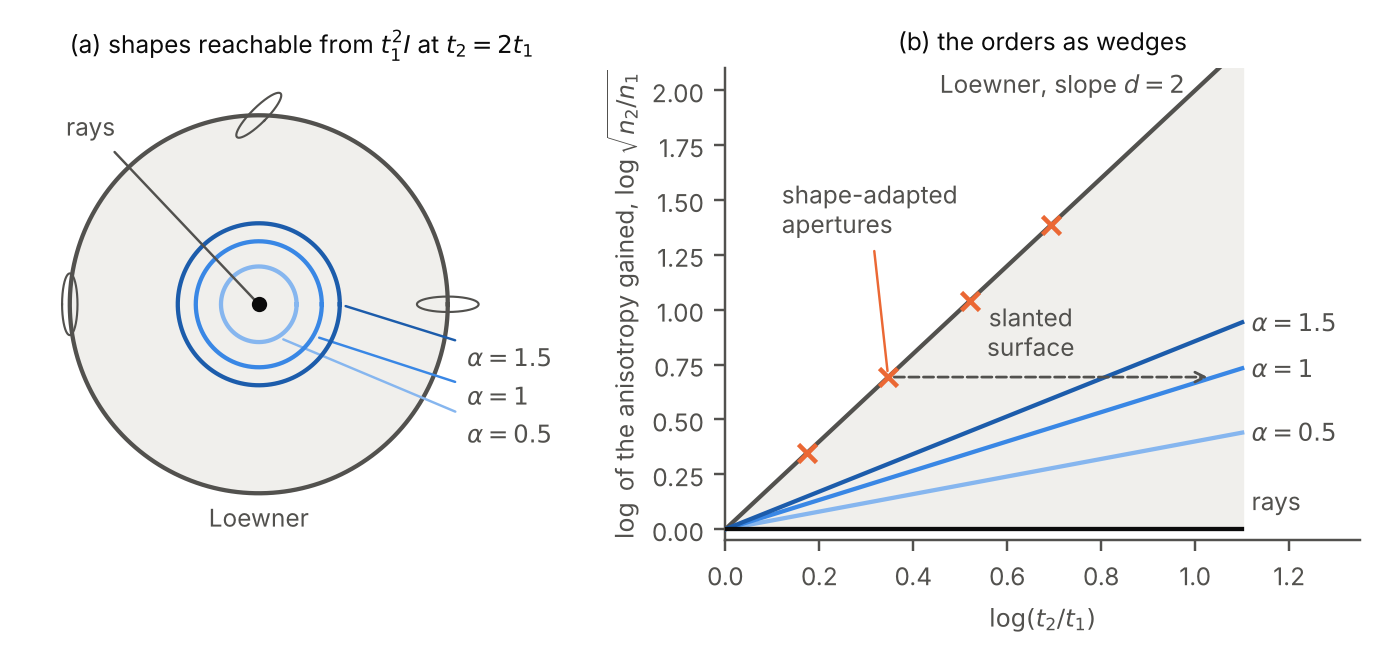
\includegraphics[width=\textwidth]{fig-shape-plane.png}
\caption{The plane, $d = 2$: one step from the isotropic aperture $\Sigma_1 = t_1^2I$. (a) The shapes
$S(\Sigma_2)$, $\det S = 1$, reachable at volume scale $t_2 = 2t_1$, in a chart whose radius is the
distance $\delta(I, S)$ of Lemma~\ref{lem:loewner-scale-shape}(4) and whose angle is twice the
orientation of the major axis.
% Round 2 (presentation review), item 10 (VERIFY-round2-structure-paper.md § 10.4): why the angle is
% doubled (det S = 1, so log S is trace-free), and the dashed arrow of panel (b), checked against
% section 4.8 and records/affine/fig-shape-plane-output.txt (y = log 2, x from 0.3466 to 1.0397).
Rotating the aperture through $\theta$ turns $\log S$, a point of the plane of trace-free symmetric
matrices, through $2\theta$, so orthogonal orientations lie at opposite points. The Loewner order reaches the disc of radius $2\sqrt2\log(t_2/t_1)$
(Lemma~\ref{lem:loewner-scale-shape}(4)); the stable order of index $\alpha$ the disc of radius
$2\sqrt2\,\frac{\alpha}{2+\alpha}\log(t_2/t_1)$ (Proposition~\ref{prop:stable-step-cone}(3)); the rays
only the centre. The ellipses are apertures on the Loewner edge in three orientations. (b) The same
orders in the logarithm of the anisotropy gained, $\sqrt{n_2/n_1}$, against the logarithm of the scale
ratio: slopes $d$, $d\alpha/(d+\alpha)$ and $0$. The crosses are the apertures of shape-adapted smoothing
at anisotropy $n_2/n_1 = 2$, $4$, $8$, $16$, reached from the
isotropic first stage (Proposition~\ref{prop:shape-adapted-apertures}), which lie on the Loewner edge.
The dashed arrow is the step for the surface at slant $60^\circ$ of \S\ref{sec:shape-adapted}, at
log-anisotropy $\log 2$. It runs from the aperture of shape-adapted smoothing on the Loewner edge to the edge of the stable order of
index $\alpha = 1$, which reaches that shape only at twice the volume scale. Computed, with the
discs checked against the two orders on random steps, by a script deposited with the paper.}
\label{fig:shape-plane}
\end{figure}

% §5.3 The landscape at a glance --- blueprint chapter 5, part 05-table.tex (Q-0288; moved forward
% to right after 5.2 in Q-0290, review flag S4: the table, with forward references, and the statement
% of thm:wedge-axis are the section's destination; the theorem's proof is 5.8, 05-wedge-axis.tex,
% after every node it reads). Included from 05-landscape.tex; the conventions are in that file's
% header. The table is built from the nodes, each cell citing the statements it summarizes; every
% cell was compared with its statements for lost hypotheses (WRITING.md § 5, "a summary drops
% hypotheses"). The table is for d >= 2, the dimension in which the general linear Loewner cell and
% the stable-order cells are stated. The one node is thm:wedge-axis; the remark on positivity is the
% plan's (notes/PLAN-article-structure.md, "§5"), as far as it is proved, and states no signed family
% (the author, 2026-10-04).
% Q-0309 (fix group 2, review flag 10): the formal statement of thm:wedge-axis moved to 5.8
% (05-wedge-axis.tex), where its vocabulary exists, before its proof; this subsection keeps the table
% and an informal statement of the theorem (the paragraph "The general linear row along the chain").

\subsection{The landscape at a glance}\label{sec:landscape-table}

Table~\ref{tab:landscape} answers, for each choice of covariance group and of the pairs of apertures
along which the record must be a further smoothing, which kernels are available. It has the groups of \S\ref{sec:scale-shape}
as rows and three orders as columns, for $d \ge 2$, and every cell has an entry, citing the statements
it summarizes in \S\S\ref{sec:invariant-wedges}--\ref{sec:smaller-groups} or in the appendices. The
cells use these terms.
\begin{itemize}
\item The \emph{ray order} relates $\Sigma$ to its multiples $c\,\Sigma$, $c \ge 1$, and $0$ to
everything.
\item The \emph{stable order} $\le_\alpha$, $0 < \alpha < 2$, relates two definite matrices when the
relative step $M = \Sigma^{-1/2}\Sigma'\Sigma^{-1/2}$ has $\lambda_{\min}(M)^{d+\alpha} \ge \det M$, and
adds the origin and the rays (Proposition~\ref{prop:similarity-stable-order-families}(1)). It lies
between the rays and the Loewner order.
% Round 3 (content review), C section 7 (VERIFY-round3-landscape-orbits-paper.md item 30): the pointer
% for "step set", which this page uses before Proposition 4.2.
It is the order of the step set (Proposition~\ref{prop:invariant-orders}, \S\ref{sec:affine-stable-cone})
of the stable orbit of index $\alpha$, the linear images $(\Sigma^{1/2})_*S_\alpha(I)$ of the isotropic $\alpha$-stable law, whose
transform is $e^{-|\omega|^\alpha}$ (Lemma~\ref{lem:elliptical-stable} and
Proposition~\ref{prop:stable-step-cone}). At $\alpha = 1$ that law is the kernel of the Poisson scale
space at unit scale (\S\ref{sec:classical-prior-art}). And it is the order generated by the cone of directions
$C_\alpha := \{X \in \PSD(d) : (d+\alpha)\,\lambda_{\min}(X) \ge \tr X\}$
(Proposition~\ref{prop:stable-order-generated}); $C_0$ gives the rays and $C_\infty := \PSD(d)$ the
Loewner order.
\item The \emph{frame} is the coordinate frame, the axes of the sampling grid along which the
positive diagonal group $\mathrm D_+(d)$ rescales. The \emph{frame's shapes} are the positive definite
diagonal matrices, the apertures whose axes are those of the frame, and they are the orbit of $I$
under $\mathrm D_+(d)$.
% Round 2 (presentation review), item 4 (VERIFY-round2-structure-paper.md § 4.1): D_s and
% Delta(Sigma), defined as in Propositions F.2 and F.4; Corr(d) is not printed in the table.
For $s \in (0,\infty)^d$ write $D_s := \diag(s_1,\dots,s_d)$, so that the frame's shapes are the
$D_s^2$, and write $\Delta(\Sigma) := \diag(\Sigma_{11},\dots,\Sigma_{dd})$ for the diagonal of $\Sigma$.
% Round 2 (presentation review), item 4: the term B-self-decomposable and sym B, as in
% Proposition 4.10.
\item The \emph{exponent cone} $\mathfrak k_\alpha$ of the stable law is the set of matrices $B$ for which
$S_\alpha(I)$ is its own image under $e^{-tB}$ convolved with a residual, for every $t > 0$. A law with
this property is \emph{$B$-self-decomposable}, or operator-self-decomposable with exponent $B$
(Proposition~\ref{prop:stable-exponent-cone}). The symmetric part of $B$ is
$\mathrm{sym}\,B := \tfrac12(B + B^{\tp})$.
\item \emph{Anisotropy} is measured by the exponent spread $\operatorname{es}$ of the non-Gaussian part,
the least $K \ge 1$ with $\psi(Q\omega) \le K\,\psi(\omega)$ for every $Q \in \Orth(d)$. It is set
against the eccentricity $\operatorname{ecc}(\Sigma)$ of the aperture, the ratio of its extreme
eigenvalues. Both are defined again where they are used, in Proposition~\ref{prop:similarity-stable-order-kernels}.
\item A non-Gaussian part is \emph{shape-blind} when it is rotation invariant at every $\Sigma$, so that
it sees the size of the aperture and not its shape. It is shape-blind \emph{at the origin} when its
\Levy{} measure has the same rate near the origin in every direction.
\item The profile entries concern a rotation-invariant law with no Gaussian part whose \Levy{}
density at $x$ is $k(|x|)\,|x|^{-d}$, with $k$ nonincreasing, its \emph{profile}, and the law is
written $\nu_k$. They use the
dilation ratio $R(\lambda) := \inf\{k(r/\lambda)/k(r) : r > 0,\ k(r) > 0\}$, $\lambda \ge 1$, and the
lower exponent $\beta_-(k) := \inf_{\lambda > 1}\log R(\lambda)/\log\lambda$
(Proposition~\ref{prop:orbit-step-cone} and Lemma~\ref{lem:dilation-ratio}).
% Round 2 (presentation review), item 4 (§ 4.2): the gloss of R(lambda) >= lambda^alpha. With
% s = r/lambda it reads k(s) s^alpha >= k(r) r^alpha for s <= r.
The condition $R(\lambda) \ge \lambda^\alpha$ for every $\lambda \ge 1$ says that $r^\alpha k(r)$ is
nonincreasing: towards the origin the profile grows at least like $r^{-\alpha}$.
\end{itemize}
The one-parameter row lies outside the scheme, a curve not being an order on $\PSD(d)$, and is listed
below the others.

\begin{table}[tp]
\centering
\small
\setlength{\tabcolsep}{4pt}
\renewcommand{\arraystretch}{1.15}
\begin{tabular}{@{}p{0.12\textwidth}p{0.27\textwidth}p{0.28\textwidth}p{0.27\textwidth}@{}}
\toprule
$G$ & rays & stable order $\le_\alpha$, $0 < \alpha < 2$ & Loewner order \\
\midrule
$\GL(d)$ &
the orbits $(\Sigma^{1/2})_*\mu_I$ of the rotation-invariant self-decomposable laws $\mu_I \ne \delta_0$,
one family for each law (Propositions~\ref{prop:ray-families} and~\ref{prop:gw-ray-families}(3)) &
% Round 3 (content review), E i and C-R3 (the author's decision D10): the cell is complete,
% Proposition 4.22(2) with C5.
the orbits of exactly the laws $N(0, aI)$, $a > 0$, and $N(0, aI) * \nu_k$, $a \ge 0$, with $k$
right-continuous and $\beta_-(k) \ge \alpha$; among the stable orbits, exactly those of index $\gamma \ge \alpha$
(Theorem~\ref{thm:wedge-axis}(3), Proposition~\ref{prop:wedge-axis-profiles},
Lemma~\ref{lem:dilation-ratio}(3)) &
the affine Gaussian scale spaces only (Theorem~\ref{thm:affine-rigidity}) \\
\addlinespace
similarities $\mathrm S(d)$ &
continuous covariant fields of symmetric self-decomposable laws over the shapes, with orbits indexed by
the normalized spectrum; the isotropic members are the rotation-invariant self-decomposable laws
$\ne \delta_0$, and none fixes its family (Proposition~\ref{prop:similarity-ray-families}) &
every family's kernels are symmetric infinitely divisible with
$\operatorname{es}(\psi_\Sigma) \le 4\operatorname{ecc}(\Sigma)^{(d+\alpha)/\alpha}$; contains the restrictions of
the $\GL(d)$ cell and of the Loewner cell, and a family in neither
(Proposition~\ref{prop:similarity-stable-order-kernels}) &
% Round 3 (content review), A.R9: F.3(4) and its witness F.3(3)(ii).
the isotropic members of the ray cell, each with a shape-blind family
(Proposition~\ref{prop:similarity-ray-families}(3)--(4)); every family's kernels are infinitely divisible with
$\operatorname{es}(\psi_\Sigma) \le 4\operatorname{ecc}(\Sigma)$
(Proposition~\ref{prop:similarity-stable-order-kernels}(2)); a uniform bound when the \Levy{} measures
at the thinnest apertures stay comparable to the isotropic member's, and none in general
(Propositions~\ref{prop:similarity-general-bounded-shape}, \ref{prop:similarity-cascade-families}
and~\ref{prop:similarity-degenerate-family}); for a profile bounded at the origin, shape-blind at the
origin (Proposition~\ref{prop:similarity-general-index-zero}) and need not be beyond it
% Round 2 (presentation review), item 4 (§ 4.3): "not beyond it" narrowed to "need not be beyond
% it"; one example family backs it, and the shape-blind families of the cell are rotation invariant.
(Proposition~\ref{prop:similarity-line-family}(3)); not every family is a Gaussian convolved with a
shape-blind part (Proposition~\ref{prop:similarity-stable-family}(3)) \\
\addlinespace
positive diagonal $\mathrm D_+(d)$ &
on the frame's shapes the images $(D_s)_*\mu_I$ of any self-decomposable $\mu_I \ne \delta_0$, not
necessarily products; orbits in $\PD(d)$ indexed by the correlation matrices; a rotation-invariant member fixes
no family off the frame's shapes (Proposition~\ref{prop:diagonal-ray-families}) &
on the frame's shapes $(D_s)_*\mu_I$ with $\mu_I$ operator-self-decomposable for every diagonal exponent
in $\mathfrak k_\alpha$, a necessary condition, and whether every such law is the isotropic member of a
family is open; strictly between the restricted Loewner cell and the ray cell, and not the union of the
restrictions of the Loewner and $\GL(d)$ cells; off the frame's shapes not described
(Proposition~\ref{prop:diagonal-stable-order-families}) &
on the frame's shapes the products $(s_1)_*\nu_1 \otimes \dots \otimes (s_d)_*\nu_d$ of self-decomposable
laws on the line (Propositions~\ref{prop:fixed-frame-families} and~\ref{prop:diagonal-ray-families}(3));
off the frame's shapes one extension, $(\Delta(\Sigma)^{1/2})_*(\nu_1 \otimes \dots \otimes \nu_d)$, the
families not described \\
\midrule
% Round 3 (content review), C-S6: what "with rotations" meant.
\multicolumn{4}{@{}p{0.98\textwidth}@{}}{\emph{One linear flow} $\{e^{sB}\}$, $B$ with a skew part allowed, along the
curve $e^{sB}\Sigma_0e^{sB^{\tp}}$: the families are the $B$-self-decomposable laws
(Proposition~\ref{prop:one-parameter-families}); for a contracting flow a rotation-invariant non-Gaussian
member exists exactly when $\tr B < (d+2)\lambda_{\min}(\mathrm{sym}\,B)$
(Proposition~\ref{prop:anisotropy-budget}).} \\
\bottomrule
\end{tabular}
\caption{The affine landscape for $d \ge 2$: the families of each group along each order. The four
corners of the scheme (Definition~\ref{def:gw-cascade-family}) are the cells of the first two rows in
the ray and the Loewner columns. Each cell cites the statements it summarizes. The cells of the general
linear group are complete, and \S\ref{sec:conclusion} says how far the others go.}
% Round 3 (content review), A.R1 and C-R2 (PLAN-review-response-paper.md R3.1, "taken unless vetoed"):
% the complete cells named in the caption, three since D10.
\label{tab:landscape}
\end{table}

\paragraph{The inclusions.} A family of a larger group or a larger order restricts to every smaller
datum, with the same kernels from scale zero (Lemma~\ref{lem:gw-kernels-from-origin}(1)), so in each column
the cells grow from the general linear row to each smaller group's row, and along each row towards the
rays. These inclusions are known to be strict:
\begin{itemize}
\item along the general linear row, at every step of the chain up to $\alpha = 2$
(Theorem~\ref{thm:wedge-axis}(3));
\item from the $\GL(d)$ cell and the restricted Loewner cell to the cell (similarities, stable order)
(Proposition~\ref{prop:similarity-stable-order-kernels}(3));
\item from the restricted Loewner cell to the stable cell, and from there to the ray cell, in the diagonal
row (Proposition~\ref{prop:diagonal-stable-order-families}(4)), and so from the restricted (diagonal,
Loewner) cell to the (diagonal, rays) cell (Proposition~\ref{prop:diagonal-ray-families}(4)).
\end{itemize}
% Round-1 external review (Gemini; PLAN-review-response-paper.md, D3): the paragraphs "The isotropic
% members" (moved to section 1, "Smaller groups") and "The general linear row along the chain" (said by
% section 1 and section 4.7) are folded into section 1.

% Q-0317 (the blind register review, second half flag 25): rem:positivity moved to section 3.4,
% beside the rigidity it is about.

% §5.4 Invariant wedges --- blueprint chapter 5, part 05-wedges.tex (Q-0288). Included from
% 05-landscape.tex; the conventions are in that file's header. The nodes are linear algebra; since
% Q-0281 wave 2, group F (the author's decision of 2026-10-05) lem:spectral-cones(2) cites C4 (ledger
% A9) in place of its compound-matrix proof, and the nodes that read it spend it. Q-0290: lem:spectral-cones, thm:cone-orders (whole, the node not
% being split; this file states its four clauses in words) and the proof of prop:invariant-orders are
% in appendix A; prop:stable-order-generated is in 5.6, after the exponent cone it reads (review flag
% S12). The prior-art paragraph cites the readings recorded in
% records/affine/READING-{lawson1989ordered,hilgert1989lie,hilgert1997causal,faraut1994analysis}.md,
% with the page anchors of the nodes' annotations; no proof depends on them. The chain of cones and
% the general linear row along it (thm:wedge-axis) are stated in 5.3.
% Q-0309 (fix group 2, review flag 35): thm:cone-orders is stated here, in place of the paraphrase of
% its four clauses, since its clause (4) defines the order thm:wedge-axis is stated on; its proof,
% lem:spectral-cones and the proof of prop:invariant-orders are in the proof appendix (app:proofs).

\subsection{Invariant wedges}\label{sec:invariant-wedges}

An order of the landscape says which changes of aperture must be further smoothings. This subsection
asks which orders there are, and how to describe one by what may happen in an instant. For the
Gaussian the answer is familiar. Its aperture may grow in any direction, $\Sigma(t)$ moving with a
positive semidefinite velocity $\Sigma'(t)$, and the pairs joined by such a curve are those of the
Loewner order (Proposition~\ref{prop:stable-order-generated}(1), at $\alpha = \infty$). The rays allow
only a velocity that is a nonnegative multiple of $\Sigma(t)$, a growth without a change of shape. An
order in between allows at each aperture a cone of velocities, the \emph{cone field}, and relates two
apertures when a curve whose velocity stays in the cones joins them. The main result,
Theorem~\ref{thm:cone-orders}, says that the closed invariant partial orders on $\PD(d)$ that arise
in this way are exactly those whose steps can be taken in fractions, and that every step of such an
order is reached along one curve, with no limit of curves needed. The rays, the stable orders and the
Loewner order are of this kind, the members $C_0$, $C_\alpha$ and $C_\infty$ of one chain of cones
(Proposition~\ref{prop:stable-order-generated}).

% Pass 6, the author's review of section 4.4 (2026-11-02; records/affine/REVIEW-author-paper-affine.md):
% "some, preferably geometric, intuition about what the cone and wedges are and how they will be
% used". Paper-only prose. The plane computation: X = [[a+u, v], [v, a-u]] has eigenvalues
% a +- r, r = sqrt(u^2+v^2); a rotation by phi rotates (u, v) by 2 phi and fixes a, a reflection
% reflects (u, v); so an O(2)-invariant closed convex cone with I in it and no line is
% {r <= k a}, k >= 0. PSD(2) is k = 1. C_alpha of prop:stable-order-generated, (2+alpha) lambda_min
% >= tr, is (2+alpha)(a-r) >= 2a, that is k = alpha/(alpha+2): C_0 has k = 0, C_2 has k = 1/2, and
% k -> 1 as alpha -> infinity. thm:wedge-axis(2) read in the plane: beta(C) = max tr X/lambda_min(X)
% - 2 = 2k/(1-k) for the round cone of opening k < 1, so (a) k > 1 (not in PSD(2)): no family;
% (b) k = 1 (a singular member): the Gaussian only; (c) k < 1: a non-Gaussian family exists iff
% beta < 2 iff k < 1/2.
\paragraph{A picture in the plane.} For $d = 2$ the cones can be drawn. Write a symmetric matrix as
$X = \bigl(\begin{smallmatrix} a+u & v \\ v & a-u \end{smallmatrix}\bigr)$, so that $\Sym(2)$ is a
space of three dimensions with coordinates $(a, u, v)$, and $X$ has the eigenvalues
$a \pm \sqrt{u^2+v^2}$. Read $X$ as the velocity of an aperture at $I$. Then $a$ is its growth in
size, $\sqrt{u^2+v^2}$ its rate of change of shape, and the angle of $(u, v)$ the direction in which
it stretches. A rotation of the plane by an angle $\phi$ rotates $(u, v)$ by $2\phi$ and leaves $a$
alone. So a closed convex cone that is invariant under rotations, contains $I$ and contains no line is
a round cone about the axis of the multiples of $I$,
\[
  \sqrt{u^2+v^2} \le k\,a \qquad \text{for some } k \ge 0 .
\]
Its opening $k$ bounds how fast the shape may change against how fast the aperture grows
(Figure~\ref{fig:cones-plane}). The rays
are the axis alone, $k = 0$. The Loewner order allows every positive semidefinite velocity, the cone
$k = 1$ of half-angle $45^\circ$, and a wider cone allows an aperture to shrink in some direction. The
cone $C_\alpha$ of the chain has $k = \alpha/(\alpha+2)$, so the stable orders, $0 < \alpha < 2$, are
the cones narrower than $k = \frac12$. The cone field carries the cone at $I$ to every aperture by the
group, and the order relates two apertures when a curve whose velocity stays in the cones joins them.
Lie theory calls a closed convex cone a \emph{wedge} (\S\ref{sec:affine-covariance}), and these
wedges, which contain no line, are the tangent objects through which it studies such orders. The rest
of the section uses them in two ways. Each affine orbit has its own set of steps along which it
cascades, and \S\S\ref{sec:affine-orbits}--\ref{sec:affine-stable-cone} find it for the orbits of
interest: the rays alone for the \Matern{} kernels, the order of $C_\gamma$ for the stable kernel of
index $\gamma$. And in the plane
Theorem~\ref{thm:wedge-axis} reads off the opening. A cone with $k < \frac12$ carries non-Gaussian
families, a cone with $\frac12 \le k \le 1$ carries only the affine Gaussian scale spaces, and a cone
with $k > 1$ carries none.

% Pass 6 (the author's request of 2026-11-02, "Add the figure please"): fig-cones-plane.png, drawn by
% records/affine/fig-cones-plane.py with its output saved (fig-cones-plane-output.txt); the script
% checks the openings k = alpha/(alpha+2), PSD(2) = {r <= a} and beta = 2k/(1-k) before drawing. No
% statement uses it.
\begin{figure}[t]
\centering
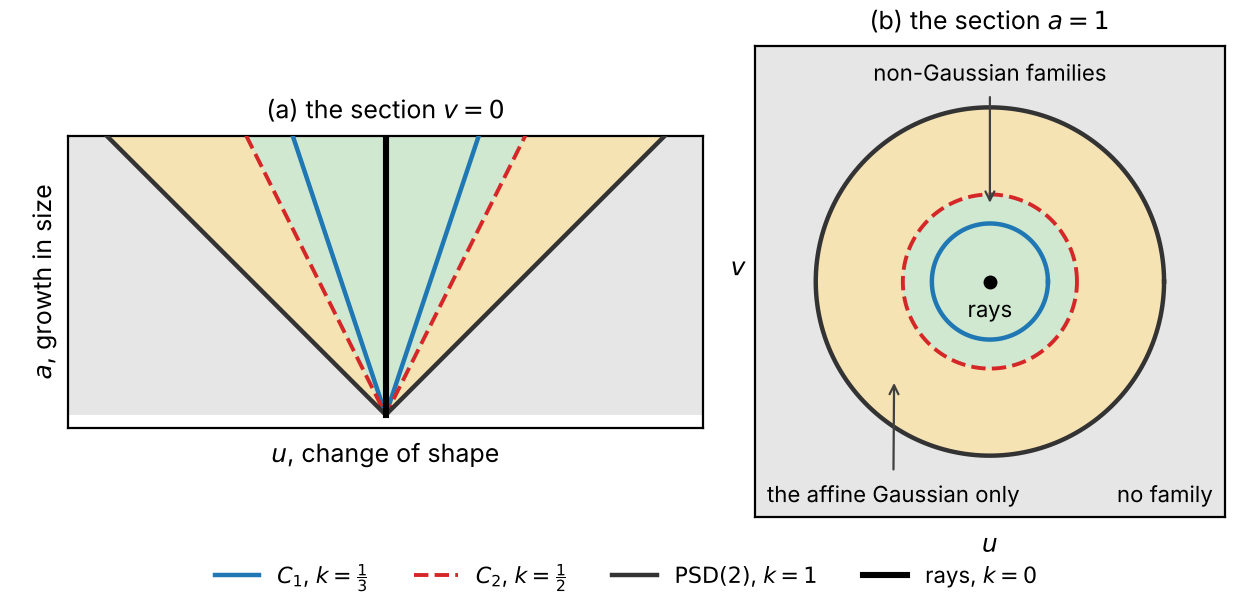
\includegraphics[width=\textwidth]{fig-cones-plane.png}
\caption{The rotation-invariant cones of velocities in the plane, in the coordinates $(a, u, v)$ of
$X = \bigl(\begin{smallmatrix} a+u & v \\ v & a-u \end{smallmatrix}\bigr)$: each is a round cone
$\sqrt{u^2+v^2} \le k\,a$ about the axis of the multiples of $I$. (a) The section $v = 0$, where each
cone is a sector. (b) The section $a = 1$, where each cone is a disc of radius $k$. Drawn are the rays
($k = 0$), the cone $C_1$ ($k = \frac13$), along whose order the orbit of the Poisson kernel cascades,
the cone $C_2$ ($k = \frac12$) and the Loewner cone $\PSD(2)$ ($k = 1$). The shading reads
Theorem~\ref{thm:wedge-axis} in the plane: a cone with $k < \frac12$ (green) carries non-Gaussian
families, one with $\frac12 \le k \le 1$ (amber) only the affine Gaussian scale spaces, and one with
$k > 1$ (grey) none. Drawn by a script deposited with the paper.}
\label{fig:cones-plane}
\end{figure}

The rest of the subsection is linear algebra, in the language of matrix analysis and of the Lie theory
of semigroups, where the orders of a homogeneous space are studied through their cones (``Prior art''
at the end of the subsection).
% Round 2 (presentation review), item 19 (VERIFY-round2-notation-paper.md § 19): the motivation of
% causal curves and of majorization, compared with Theorem 4.3(1) (the test log M in C is its
% conclusion, the order being defined by curves) and Lemma C.1(2), (5).
An order is described by its set of relative steps $M = \Sigma^{-1/2}\Sigma'\Sigma^{-1/2}$
(Proposition~\ref{prop:invariant-orders}), and an $\Orth(d)$-invariant closed convex cone $C$ of symmetric matrices plays
the part of the allowed velocities, through the cone field of Theorem~\ref{thm:cone-orders}. A single
step is tested by its logarithm: Theorem~\ref{thm:cone-orders}(1) shows that a curve of that cone
field joins $\Sigma$ to $\Sigma'$ exactly when $\log M \in C$. Steps do not compose by multiplication.
The composite of two steps $M$ and $N$ is $M^{1/2}N'M^{1/2}$ with $N'$ a rotation of $N$
(Proposition~\ref{prop:invariant-orders}(3)), and its logarithm is not $\log M + \log N'$ when $M$
and $N'$ do not commute. So it is not obvious that the test is transitive. A comparison of spectra by partial sums,
majorization, bounds the spectrum of the composite whatever the relative position of the eigenframes,
with one cited inequality (C4, Theorem~\ref{thm:cited-A9}). It gives both the transitivity and the
fact that a curve of the cone field ends at a step in $\exp C$.
Proposition~\ref{prop:invariant-orders} sets up the dictionary between invariant orders and sets of
steps in which the theorem is stated.

% shared with blueprint prop:invariant-orders
\begin{proposition}[invariant relations on $\PD(d)$ and their steps]\label{prop:invariant-orders}
Let $d \ge 1$ and write $\Sym(d)$ for the real symmetric $d \times d$ matrices. Call a set
$\mathcal K \subseteq \PD(d)$ a \emph{step set} if $QMQ^{\tp} \in \mathcal K$ whenever $M \in \mathcal K$
and $Q \in \Orth(d)$. For a step set write $\Sigma \le_{\mathcal K} \Sigma'$, for
$\Sigma, \Sigma' \in \PD(d)$, when the \emph{relative step} $\Sigma^{-1/2}\Sigma'\Sigma^{-1/2}$ lies in
$\mathcal K$, and put $\mathcal S_{\mathcal K} := \{A \in \GL(d) : AA^{\tp} \in \mathcal K\}$.
\begin{enumerate}
\item \emph{(Invariant relations are step sets.)} For $\Sigma, \Sigma' \in \PD(d)$ and every
$A \in \GL(d)$ with $AA^{\tp} = \Sigma$, $\Sigma \le_{\mathcal K} \Sigma'$ if and only if
$A^{-1}\Sigma'A^{-\tp} \in \mathcal K$. The relation $\le_{\mathcal K}$ is $\GL(d)$-invariant:
$\Sigma \le_{\mathcal K} \Sigma'$ if and only if $B\Sigma B^{\tp} \le_{\mathcal K} B\Sigma'B^{\tp}$, for
every $B \in \GL(d)$. Every $\GL(d)$-invariant relation $R$ on $\PD(d)$ is $\le_{\mathcal K}$ for
exactly one step set, $\mathcal K = \{M \in \PD(d) : I \,R\,M\}$.
\item \emph{(Order properties.)} $\le_{\mathcal K}$ is reflexive if and only if $I \in \mathcal K$; it is
antisymmetric if and only if no $M \ne I$ has both $M$ and $M^{-1}$ in $\mathcal K$; and it is closed in
$\PD(d) \times \PD(d)$ if and only if $\mathcal K$ is closed in $\PD(d)$.
\item \emph{(How steps compose.)} If $\Sigma \le_{\mathcal K} \Sigma' \le_{\mathcal K} \Sigma''$, $M$ is
the relative step of $(\Sigma, \Sigma')$ and $N$ that of $(\Sigma', \Sigma'')$, then the relative step
of $(\Sigma, \Sigma'')$ is $M^{1/2}N'M^{1/2}$ with $N' = Q^{\tp}NQ$ for some $Q \in \Orth(d)$, and its
eigenvalues are those of $MN'$. Conversely, for $M, N \in \mathcal K$ the triple $I$, $M$,
$M^{1/2}NM^{1/2}$ is such a chain. So $\le_{\mathcal K}$ is transitive if and only if
$M^{1/2}NM^{1/2} \in \mathcal K$ for all $M, N \in \mathcal K$, if and only if $\mathcal S_{\mathcal K}$
is closed under products. The spectrum of the composite is not determined by the spectra of the two
steps: for $d = 2$ the step $\diag(4,1)$ followed by $\diag(4,1)$ gives $\diag(16,1)$, and followed by
$\diag(1,4)$ gives $4I$.
\item \emph{(The infinitesimal cone.)} The set
$C(\mathcal K) := \{X \in \Sym(d) : e^{tX} \in \mathcal K \text{ for every } t \ge 0\}$ is invariant
under $X \mapsto QXQ^{\tp}$, $Q \in \Orth(d)$, and under $X \mapsto cX$, $c \ge 0$. It is closed when
$\mathcal K$ is closed in $\PD(d)$, and if $\le_{\mathcal K}$ is antisymmetric then
$X \in C(\mathcal K)$ and $-X \in C(\mathcal K)$ only for $X = 0$.
\end{enumerate}
\end{proposition}

Clause (1) is the dictionary between the orders of the scheme and sets of matrices: a
$\GL(d)$-invariant order on $\PD(d) = \GL(d)/\Orth(d)$ is its set of relative steps at $I$.
The proof is in Appendix~\ref{app:wedge-axis}.

The invariant cones are read through their eigenvalues. For $X \in \Sym(d)$ write
$\lambda^\uparrow(X)$ for its eigenvalues in increasing order, and for a cone $C \subseteq \Sym(d)$
put $\exp C := \{e^X : X \in C\}$.

An invariant cone generates an order along curves that move in the cone at each point. The theorem
says which orders arise in this way, and its clause (4) gives the orders on $\PSD(d)$ along which the
general linear row is read in \S\ref{sec:wedge-axis-proof}.

% CHANGED Q-0281 wave 2: blind review W2F-4 (the sentence above) and W2F-5 (the parenthetical of clause
% (3), mirrored from the blueprint statement).
% shared with blueprint thm:cone-orders
\begin{theorem}[invariant orders generated by cone fields]\label{thm:cone-orders}
Let $d \ge 1$ and let $C \subseteq \Sym(d)$ be a closed convex cone invariant under $X \mapsto QXQ^{\tp}$,
$Q \in \Orth(d)$. Its \emph{cone field} assigns to $\Sigma \in \PD(d)$ the cone
$\Sigma^{1/2}C\Sigma^{1/2}$ of tangent vectors, which equals $ACA^{\tp}$ for every $A$ with
$AA^{\tp} = \Sigma$, so that $B(\Sigma^{1/2}C\Sigma^{1/2})B^{\tp}$ is the cone at $B\Sigma B^{\tp}$ for
$B \in \GL(d)$. An absolutely continuous $\gamma : [0,1] \to \PD(d)$ is \emph{$C$-causal} if
$\gamma(t)^{-1/2}\gamma'(t)\gamma(t)^{-1/2} \in C$ for almost every $t$; write $\Sigma \preceq_C \Sigma'$
when a $C$-causal curve runs from $\Sigma$ to $\Sigma'$. Use the notation of Proposition~\ref{prop:invariant-orders}
(step sets $\mathcal K$, their relations $\le_{\mathcal K}$, the sets $\mathcal S_{\mathcal K}$ and the cones
$C(\mathcal K)$), write $\exp C := \{e^X : X \in C\}$, and write $\lambda^\uparrow_1(M)$ for the least
eigenvalue of $M$.
\begin{enumerate}
\item \emph{(The order of a cone field.)} $\Sigma \preceq_C \Sigma'$ if and only if the relative step
$M = \Sigma^{-1/2}\Sigma'\Sigma^{-1/2}$ lies in $\exp C$, and then $\gamma(t) := \Sigma^{1/2}M^t\Sigma^{1/2}$
is $C$-causal. So $\preceq_C$ is $\le_{\exp C}$: a closed $\GL(d)$-invariant preorder, which is a partial
order if and only if $C \cap (-C) = \{0\}$; and $C(\exp C) = C$.
\item \emph{(Closed invariant orders.)} Let $\mathcal K$ be a closed step set for which $\le_{\mathcal K}$
is a partial order. Then
$\{B \in \gl(d) : e^{tB} \in \mathcal S_{\mathcal K} \text{ for every } t \ge 0\} =
\{B : \tfrac12(B + B^{\tp}) \in C(\mathcal K)\}$, and this is a closed convex cone containing every
skew-symmetric matrix; $C(\mathcal K)$ is an $\Orth(d)$-invariant closed convex cone with
$C(\mathcal K) \cap (-C(\mathcal K)) = \{0\}$; and $\preceq_{C(\mathcal K)}$ is contained in
$\le_{\mathcal K}$. The following are equivalent: (a) $\le_{\mathcal K}$ is $\preceq_{C'}$ for some cone
$C'$ as above; (b) $\mathcal K = \exp C(\mathcal K)$; (c) $M^\tau \in \mathcal K$ whenever
$M \in \mathcal K$ and $0 \le \tau \le 1$. When they hold, $C' = C(\mathcal K)$.
\item \emph{(A closed order without a cone.)} $\mathcal K := \{I\} \cup \{M \in \PD(d) :
\lambda^\uparrow_1(M) \ge 2\}$ is a closed step set, $\le_{\mathcal K}$ is a partial order, and
$C(\mathcal K) = \{0\}$, so that $\preceq_{C(\mathcal K)}$ is equality; hence $\le_{\mathcal K}$ is
$\preceq_{C'}$ for no cone $C'$.
\item \emph{(On $\PSD(d)$.)} Suppose $I \in C$ and $C \cap (-C) = \{0\}$. For $\Sigma, \Sigma' \in
\PSD(d)$ let $\Sigma \preceq^+_C \Sigma'$ when $\Sigma = 0$, or $\Sigma' = c\,\Sigma$ for some $c \ge 1$,
or $\Sigma, \Sigma' \in \PD(d)$ and $\Sigma \preceq_C \Sigma'$. Then $\preceq^+_C$ is a $\GL(d)$-invariant
partial order on $\PSD(d)$ that contains the rays, every pair $\Sigma \preceq^+_C \Sigma'$ is joined by a
chain as in Theorem~\ref{thm:cascade-infinitely-divisible}(2), and $(G, \preceq^+_C)$ is a wedge datum with the
path condition (P) for every closed subgroup $G$ of $\GL(d)$ containing the dilations. It is contained in
the Loewner order if and only if $C \subseteq \PSD(d)$. For $C = \{cI : c \ge 0\}$ it is the ray order of
Definition~\ref{def:gw-cascade-family}.
\end{enumerate}
\end{theorem}

So an $\Orth(d)$-invariant closed convex cone generates an invariant preorder whose steps are exactly
the exponentials of the cone, and a partial order when $C \cap (-C) = \{0\}$. The steps are reached along the geodesics $\Sigma^{1/2}M^t\Sigma^{1/2}$, and
no closure is needed. A closed invariant order comes from a cone exactly when its steps are closed
under fractional powers, and clause (3) shows that the restriction is needed: a closed invariant
order can have no infinitesimal part at all. At $C = \PSD(d)$, clause (4) adds to the Loewner order of
$\PD(d)$ only the origin and the rays. It is therefore smaller than the Loewner order of $\PSD(d)$,
which also has steps from nonzero singular matrices to definite ones. The proof, in
Appendix~\ref{app:wedge-axis}, runs through one family of functionals, which
Lemma~\ref{lem:spectral-cones} makes superadditive along any three points.

A vector $x \in \RR^d$ is \emph{majorized} by $y$ when, for every $k$, the sum of the $k$ smallest
entries of $x$ is at least that of $y$, with equal totals: $x$ is the less spread of the two.
% Round 3 (content review), C-S3: Bhatia states (III.21) through the largest entries.
The source of C4 states its inequality in the equivalent form of partial sums of the largest entries
(\S\ref{sec:cited-facts}). Two matrix inequalities
carry the correspondence. The eigenvalues of a sum $X + Y$ are majorized by the sum of the two
spectra, and the logarithmic spectrum of a product $M^{1/2}NM^{1/2}$ by the sum of the logarithmic
spectra of $M$ and $N$. Clause (3) of Proposition~\ref{prop:invariant-orders} is the reason
majorization is the tool here: the spectrum of a composite is not a function of the two spectra, but
majorization bounds it uniformly over the rotation between the eigenframes.
Lemma~\ref{lem:spectral-cones} states the two inequalities, proves the first, and derives the second
from the cited fact C4 and a determinant, with the description of the $\Orth(d)$-invariant closed
convex cones by symmetric cones of eigenvalues and the transitivity of $\le_{\exp C}$. It is in
Appendix~\ref{app:wedge-axis}, with the proofs it serves.

The cones that matter here form one chain, from the rays to the Loewner order:
$C_\alpha := \{X \in \PSD(d) : (d+\alpha)\,\lambda_{\min}(X) \ge \tr X\}$ for $0 \le \alpha < \infty$, and
$C_\infty := \PSD(d)$. Its members of index $0 < \alpha < 2$ are the symmetric parts of the exponent
cones of the stable laws, and Proposition~\ref{prop:stable-order-generated} in \S\ref{sec:affine-stable-cone} shows that
their orders are the stable orders.

\paragraph{Prior art.} The correspondence between invariant cone fields, Lie wedges, semigroups and
closed orders on a homogeneous space $G/H$ is Lawson's (\sscite{lawson1989ordered}, Thm.~4.9, p.~290;
Props.~6.3--6.4, pp.~295--296; Thms.~7.4--7.5, pp.~300--302), on the Lie theory of semigroups of
Hilgert, Hofmann and Lawson (\sscite{hilgert1989lie}, Prop.~V.1.7, pp.~375--376). Read on $\GL(d)$
with the involution $A \mapsto A^{-\tp}$, their Cor.~V.4.58 (p.~440) gives the transitivity of
Theorem~\ref{thm:cone-orders}(1) for pointed cones, and their abelian example (p.~376) is the model of
Theorem~\ref{thm:cone-orders}(3). Hilgert and \'Olafsson state the bijection between invariant regular
cones and invariant regular causal structures (\sscite{hilgert1997causal}, Thm.~2.2.2, p.~40), and the dual
description of a closed convex cone is in Faraut and Kor\'anyi (\sscite{faraut1994analysis},
Thm.~I.1.1, p.~2).
% Round 3 (content review), C-R4, D-R7 (VERIFY-round3-landscape-orbits-paper.md item 11; the author's
% decision D13): no priority claim. "Which is not connected" dropped, the powers-versus-roots reason
% kept. Lawson 1994 acquired and read at the page (D13; records/affine/READING-lawson1994polar.md): his
% Thm. 3.1 has the closedness and the wedges that are not pointed, so the former contrast with Cor. V.4.58
% ("needs no closure ... the cones need not be pointed") went. Hilgert-Neeb 1993, Neeb 2000 and Kostant are
% not held, and nothing is said against them.
Here the correspondence is read on $\PD(d)$ through step sets and their spectra and proved by
majorization. The semigroup is in Lawson's paper on polar decompositions, which allows cones that are
not pointed and derives the closedness that Cor.~V.4.58 asks for: $\mathcal S_{\exp C} = (\exp C)\Orth(d)$ is a
closed semigroup with subtangent wedge $C \oplus \mathfrak{so}(d)$, by his Thm.~3.1
(\sscite{lawson1994polar}, pp.~198--199), as $\operatorname{ad}X$ has real spectrum for symmetric $X$ (his
Lem.~4.1 and Example~4.2, p.~203) and the centre of $\gl(d)$ is $\RR I$, which gives his condition (4). By
Proposition~\ref{prop:invariant-orders}(3) that is the transitivity of $\le_{\exp C}$. His paper has no order on the quotient. The characterization by powers is the
form on $\PD(d)$ of their theorem that a closed subsemigroup of a connected Lie group is divisible,
with roots of every order, exactly when it is the exponential image of its tangent wedge, the
set of generators of the one-parameter semigroups it contains
(\sscite{hilgert1989lie}, Thm.~V.6.5, p.~460). Their divisibility asks for roots of the elements of
$\mathcal S_{\mathcal K}$, while the powers in (c) are those of the positive definite steps. The two agree
only on the symmetric elements. The proof here is by majorization. As orders, the stable
orders are the Loewner order in other coordinates (Proposition~\ref{prop:stable-order-generated}(3)), and
this paper reads them as the orders of the stable orbits (Proposition~\ref{prop:stable-step-cone}).

% §5.5 The base, and §5.6 the wedge of an orbit --- blueprint chapter 5, part 05-orbits.tex (Q-0288).
% Included from 05-landscape.tex; the conventions are in that file's header. Order: the blueprint's.
% The stable rung comes first in 5.6 because prop:orbit-step-cone reads prop:stable-step-cone;
% prop:stable-order-generated (blueprint part 05-wedges) follows prop:stable-exponent-cone, whose cone
% it reads (Q-0290, review flag S12). The two Matern cross-shape nodes and the grid remark are in
% appendix B, three routine proofs in appendix E (Q-0290). The six [A] nodes all rest on A3(iii),
% named once at the start of 5.6 (the review's length judgement). The identification of the Matern
% orbit with the anisotropic Matern of spatial statistics is a
% naming read at the page (records/affine/READING-whittle1954stationary.md,
% READING-lindgren2011explicit.md), not a fact a proof rests on.

\subsection{The base: the general linear group along rays}\label{sec:affine-orbits}

The smallest order of the scheme is the ray order. It requires only that the record at
$\lambda^2\Sigma$, $\lambda > 1$, be a further smoothing of the record at $\Sigma$: a zoom out without
a change of shape. This subsection asks which kernels can then be carried to every elliptical aperture
covariantly under the whole general linear group, and the answer is that this costs nothing beyond
what the isotropic theory requires. The kernel $\mu_I$ at the round aperture fixes the family, which is
its \emph{affine orbit}: the kernel at $\Sigma$ is $(\Sigma^{1/2})_*\mu_I$, the round kernel stretched
by $\Sigma^{1/2}$, as the Gaussian of covariance $2b\Sigma$ is the round Gaussian of covariance $2bI$
stretched. The orbit is a family along the rays exactly when $\mu_I$ is rotation invariant and
self-decomposable \ref{eq:self-decomposable} (Proposition~\ref{prop:ray-families}). The
rotation-invariant self-decomposable laws other than $\delta_0$ are the kernels from scale zero of the
isotropic families (Theorem~\ref{thm:isotropic-classification} and
Lemma~\ref{lem:radial-marginal}(1)), so every isotropic scale space, the stable and the \Matern{} ones
among them, has an affine orbit along the rays. What a non-Gaussian orbit cannot do is cascade along a
step that widens the aperture in some directions and not in others, a step of rank below $d$
(Proposition~\ref{prop:affine-orbits}(3)). The \Matern{} orbit of
Proposition~\ref{prop:affine-orbits}(4) is the example to keep in mind.

% shared with blueprint prop:affine-orbits
\begin{proposition}[affine orbits of isotropic laws]\label{prop:affine-orbits}
Let $d \ge 1$ and let $g : [0,\infty) \to [0,\infty)$ be continuous with $g(0) = 0$ and such that
$\omega \mapsto e^{-g(|\omega|^2)}$ is the characteristic function of a probability measure
$\mu_I$ on $\RR^d$. For $\Sigma \in \PD(d)$ put $\mu_\Sigma := (\Sigma^{1/2})_*\mu_I$, the
\emph{affine orbit} of $\mu_I$.
\begin{enumerate}
\item \emph{(Covariance.)} $\widehat\mu_\Sigma(\omega) = e^{-g(\langle\omega,\Sigma\omega\rangle)}$,
and $A_*\mu_\Sigma = \mu_{A\Sigma A^{\tp}}$ for every $A \in \GL(d)$ and $\Sigma \in \PD(d)$.
\item \emph{(Cascade along rays.)} If for some $\lambda > 1$ there is a probability measure
$\nu_\lambda$ on $\RR^d$ with $e^{-g(\lambda^2|\omega|^2)} = e^{-g(|\omega|^2)}\,\widehat\nu_\lambda(\omega)$,
then $\mu_{\lambda^2\Sigma} = \mu_\Sigma * (\Sigma^{1/2})_*\nu_\lambda$ for every
$\Sigma \in \PD(d)$.
\item \emph{(No cascade across shapes.)} If $d \ge 2$ and $g$ is not linear, then for no
$\Sigma \in \PD(d)$ and no $P \in \PSD(d)$ with $0 < \rank P < d$ is
$\mu_{\Sigma+P} = \mu_\Sigma * \rho$ with $\rho$ a probability measure. In particular the orbit is
not the family of kernels from scale zero of any affine cascade family.
\item \emph{(The \Matern{} orbits.)} For $\gamma > 0$, $g_\gamma(u) := \gamma\log(1+u)$ satisfies
the hypothesis in every dimension: $(1+|\omega|^2)^{-\gamma}$ is the characteristic function of
the law of $\sqrt{2V}\,Z$, with $V$ Gamma distributed of shape $\gamma$ and scale $1$ and $Z$
standard normal on $\RR^d$, independent. Its orbit has
$\widehat\mu_\Sigma(\omega) = (1 + \langle\omega,\Sigma\omega\rangle)^{-\gamma}$; clause (3)
applies to it, $g_\gamma$ not being linear; and the hypothesis of clause (2) holds for every
$\gamma > 0$ and every $\lambda > 1$, with $\nu_\lambda$ the law of $\sqrt{2Y}\,Z$, where $Z$ is
standard normal on $\RR^d$ and $Y \ge 0$, independent of $Z$, is compound Poisson with \Levy{}
measure $\gamma\,(e^{-x/\lambda^2} - e^{-x})\,x^{-1}dx$ on $(0,\infty)$, of total mass
$2\gamma\log\lambda$.
\end{enumerate}
\end{proposition}

Clause (3) is Theorem~\ref{thm:rank-deficient-step} read on the orbit. The stable orbit
$e^{-\langle\omega,\Sigma\omega\rangle^{\alpha/2}}$, $0 < \alpha < 2$, is another instance of the
proposition (Lemma~\ref{lem:elliptical-stable}), so by clause (3) it is not a family along the Loewner
order. For $\gamma > d/2$ the family of clause (4) is the \Matern{} covariance of spatial statistics
(\sscite{matern1960spatial}, (2.4.5)--(2.4.7), pp.~17--18; \sscite{whittle1954stationary}, \S9,
pp.~447--448; \sscite{lindgren2011explicit}, \S2.1, eqs.~(1)--(2), p.~426), with geometric anisotropy
(\sscite{lindgren2011explicit}, \S3.4, p.~437), in which the matrix is a parameter of the covariance. Clause (3) excludes
the rank-deficient steps between two values of it, and Proposition~\ref{prop:matern-steps} shows that
no step across shapes has a positive increment.
The proof is in Appendix~\ref{app:proofs}.


The converse holds: a family covariant under the general linear group that cascades along the ray of
$I$ is such an orbit, and the law must be self-decomposable.

% shared with blueprint prop:ray-families+663841edc318
\begin{proposition}[the ray families are the orbits of the self-decomposable isotropic laws]\label{prop:ray-families}
Let $d \ge 1$ and let $(\mu_\Sigma)_{\Sigma\in\PD(d)}$ be probability measures on $\RR^d$ with
\begin{enumerate}
\item[(R1)] \emph{(affine covariance)} $A_*\mu_\Sigma = \mu_{A\Sigma A^{\tp}}$ for every
$A \in \GL(d)$ and $\Sigma \in \PD(d)$;
\item[(R2)] \emph{(a cascade along the ray of $I$)} for every $\lambda > 1$ there is a probability
measure $\rho_\lambda$ on $\RR^d$ with $\mu_{\lambda^2I} = \mu_I * \rho_\lambda$.
\end{enumerate}
Then $\mu_I$ is rotation invariant and self-decomposable \ref{eq:self-decomposable},
$\mu_\Sigma = (\Sigma^{1/2})_*\mu_I$ for every $\Sigma$, and the family cascades along every ray:
$\mu_{\lambda^2\Sigma} = \mu_\Sigma * (\Sigma^{1/2})_*\rho_\lambda$ for every $\Sigma \in \PD(d)$
and $\lambda > 1$. Conversely, for every rotation-invariant self-decomposable law $\mu_I$ on
$\RR^d$ the family $\mu_\Sigma := (\Sigma^{1/2})_*\mu_I$ satisfies (R1) and (R2).
\end{proposition}

With Theorem~\ref{thm:affine-rigidity} this places the obstruction for $d \ge 2$: along the rays every
rotation-invariant self-decomposable law keeps its orbit, and across every step of the Loewner order
only the Gaussian does. Which steps across shapes
an orbit survives depends on the law, and that is the next subsection.

% proof of prop:ray-families
\begin{proof}
(R1) is (K3) of Definition~\ref{def:affine-cascade-family} for the kernels from scale zero, and (R2)
is (K1) along the ray of $I$ alone.

\emph{Covariance determines the orbit.} (R1) with $A = Q \in \Orth(d)$ and $\Sigma = I$ gives
$Q_*\mu_I = \mu_{QQ^{\tp}} = \mu_I$, and with $A = \Sigma^{1/2}$ it gives
$(\Sigma^{1/2})_*\mu_I = \mu_\Sigma$, as for the orbits of Proposition~\ref{prop:affine-orbits}.

\emph{Self-decomposability.} By (R1) with $A = \lambda I$, $\mu_{\lambda^2I} = (\lambda I)_*\mu_I$,
so (R2) reads $(\lambda I)_*\mu_I = \mu_I * \rho_\lambda$. Applying $(\lambda^{-1}I)_*$ gives
$\mu_I = (cI)_*\mu_I * (cI)_*\rho_\lambda$ with $c := \lambda^{-1}$, which is
\ref{eq:self-decomposable} with the residual $(cI)_*\rho_\lambda$, and every $c \in (0,1)$ arises.

\emph{Every ray.} $\mu_{\lambda^2\Sigma} = (\Sigma^{1/2})_*\mu_{\lambda^2I}
= (\Sigma^{1/2})_*(\mu_I * \rho_\lambda) = \mu_\Sigma * (\Sigma^{1/2})_*\rho_\lambda$.

\emph{Converse.} For (R1), let $B := A\Sigma^{1/2}$ and $\Sigma' := A\Sigma A^{\tp} = BB^{\tp}$. Then
$Q := \Sigma'^{-1/2}B$ is orthogonal, so
$A_*\mu_\Sigma = B_*\mu_I = (\Sigma'^{1/2})_*Q_*\mu_I = \mu_{\Sigma'}$. For (R2), self-decomposability
at $c := \lambda^{-1}$ gives $\mu_I = (cI)_*\mu_I * \rho_c$, and applying $(\lambda I)_*$ gives
$\mu_{\lambda^2I} = \mu_I * (\lambda I)_*\rho_c$.
\end{proof}

\subsection{The step set of an orbit}\label{sec:affine-stable-cone}

Shape adaptation changes the shape of the aperture as the scale grows (\S\ref{sec:landscape-uses}, the third use).
For the Gaussian every Loewner step is a further smoothing, so the shape may change as fast as
Lemma~\ref{lem:loewner-scale-shape}(3) allows: in the plane, a step that doubles the volume scale
reaches an anisotropy gained of $4$ and no more. This subsection asks the same of the other affine
orbits. Along which steps $\Sigma \to \Sigma'$ across shapes is the kernel at $\Sigma'$ the kernel at
$\Sigma$ convolved with a probability measure? Along those steps the coarser record is a further
smoothing of the finer one, and along every other step a change of shape is a re-measurement of the
image.

To state the question for every orbit, relate two apertures $\Sigma, \Sigma' \in \PD(d)$
when $\mu_{\Sigma'} = \mu_\Sigma * \rho$ for a positive finite measure $\rho$. The orbit is covariant
under $\GL(d)$ (Proposition~\ref{prop:affine-orbits}(1)), so this relation is $\GL(d)$-invariant, and by
Proposition~\ref{prop:invariant-orders}(1) it is $\le_{\mathcal K}$ for exactly one step set
$\mathcal K$: the set of $M$ with $\mu_M = \mu_I * \rho$. Call $\mathcal K$ the \emph{step set} of the
orbit. It contains the rays exactly when $\mu_I$ is self-decomposable
(Proposition~\ref{prop:ray-families}). For a non-Gaussian orbit it contains no step
$\Sigma \to \Sigma + P$ with $0 < \rank P < d$ (Proposition~\ref{prop:affine-orbits}(3)), so the
question is about steps of full rank.

The answer depends on the kernel. The orbit of the isotropic $\alpha$-stable law, $0 < \alpha < 2$,
cascades on full-rank steps of every orientation, under a speed limit of the Gaussian's form and
narrower: with $t_1, t_2$ the volume scales of the two apertures, the anisotropy gained is at most
$(t_2/t_1)^{d\alpha/(d+\alpha)}$, against $(t_2/t_1)^d$ for the Gaussian
(Proposition~\ref{prop:stable-step-cone}(3) and Lemma~\ref{lem:loewner-scale-shape}(3)). For the
Poisson kernel, $\alpha = 1$ (\S\ref{sec:classical-prior-art}), a step in the plane that doubles the
volume scale reaches an anisotropy gained of $2^{2/3} \approx 1.59$ and no more, and
Figure~\ref{fig:shape-plane} draws both limits. At the other end, the \Matern{} orbits cascade along
the rays and along no other step (Proposition~\ref{prop:matern-steps}). No orbit whose transform falls
off like a power of the frequency, in the sense of Proposition~\ref{prop:log-orbit-rays}, has a
positive increment on a step off the rays, and the orbits of decaying rational symbols are among them
(Proposition~\ref{prop:rational-symbols}). For the orbit of a general profile, one function of the
profile, its dilation ratio, gives a set of steps on which the orbit cascades
(Proposition~\ref{prop:orbit-step-cone}); whether it cascades on more steps is open. The subsection
ends with what the theorem on the general linear row (\S\ref{sec:wedge-axis-proof}) takes from the
orbits: the exponents of the isotropic stable law, the bound they put on a non-Gaussian law, and the
stable order extended to $\PSD(d)$.

The answers are read through the \Levy--Khintchine representation (C2, Theorem~\ref{thm:cited-A3}),
and from here on the subsection uses its vocabulary. The kernels of the stable orbits and of the
orbits of Proposition~\ref{prop:orbit-step-cone} are \emph{infinitely divisible} laws with no
Gaussian part. Each is the law of a sum of independent displacements, and its \emph{\Levy{} measure}
gives the expected number of displacements of each size and direction. Here that measure has a
density $n_\Sigma(x)$, the rate of the displacements per unit volume, not the density of the kernel.
A step $\Sigma \to \Sigma'$ is a further smoothing when the kernel at $\Sigma'$ has at least the rate
of displacements of the kernel at $\Sigma$ at every size and in every direction,
$n_\Sigma \le n_{\Sigma'}$ (Proposition~\ref{prop:orbit-step-cone}(2)), and for the stable orbits only
then (Proposition~\ref{prop:stable-step-cone}(1)).

\subsubsection*{The stable rung}

The chain of cones $C_\alpha$ of \S\ref{sec:invariant-wedges} is a ladder from the rays ($\alpha = 0$)
to the Loewner order ($\alpha = \infty$). Call the \emph{rung} of an orbit the largest index $\alpha$
whose stable order its step set contains. The elliptical stable laws are built from their \Levy{}
densities.

% shared with blueprint lem:elliptical-stable
\begin{lemma}[the elliptical stable laws]\label{lem:elliptical-stable}
Let $d \ge 1$ and $0 < \alpha < 2$, and put
\[
  c_{d,\alpha} := \int_{\RR^d}(1 - \cos y_1)\,|y|^{-d-\alpha}\,dy .
\]
Then $0 < c_{d,\alpha} < \infty$. For $H \in \PD(d)$ and $x \in \RR^d \setminus \{0\}$ put
\begin{equation}\label{eq:stable-levy-density}
  n_H(x) := c_{d,\alpha}^{-1}(\det H)^{-1/2}\langle x,H^{-1}x\rangle^{-(d+\alpha)/2} ,
  \qquad \psi_H(\omega) := \langle\omega,H\omega\rangle^{\alpha/2} .
\end{equation}
\begin{enumerate}
\item For every $H \in \PD(d)$ and $\omega \in \RR^d$,
$\psi_H(\omega) = \int_{\RR^d\setminus\{0\}}(1 - \cos\langle\omega,x\rangle)\,n_H(x)\,dx$, and
$\int_{\RR^d\setminus\{0\}}(|x|^2 \wedge 1)\,n_H(x)\,dx < \infty$.
\item For every $H \in \PD(d)$ there is a unique probability measure $S_\alpha(H)$ on $\RR^d$ with
$\widehat{S_\alpha(H)} = e^{-\psi_H}$. It is infinitely divisible with generating triplet
$(0, n_H(x)\,dx, 0)$, and $A_*S_\alpha(H) = S_\alpha(AHA^{\tp})$ for every $A \in \GL(d)$.
\item $n_{AHA^{\tp}}(x) = |\det A|^{-1}\,n_H(A^{-1}x)$ for $A \in \GL(d)$, $H \in \PD(d)$ and
$x \ne 0$.
\end{enumerate}
In particular $g(u) := u^{\alpha/2}$ satisfies the hypothesis of Proposition~\ref{prop:affine-orbits}, with
$\mu_I = S_\alpha(I)$, and the affine orbit of $S_\alpha(I)$ is $\mu_\Sigma = S_\alpha(\Sigma)$, the
\emph{stable orbit}.
\end{lemma}

The law $S_\alpha(H)$ is the rotation-invariant $\alpha$-stable law (\sscite{sato1999levy}, Thm.~14.14,
p.~86) transported by $H^{1/2}$, with its constant normalized to $1$. In the terms of Samorodnitsky
and Taqqu it is a sub-Gaussian stable law. The existence in (2) is their Proposition~2.5.2 with
$R = 2H$, and their Proposition~2.5.7 makes every such law a linear image of $S_\alpha(I)$
(\sscite{samorodnitsky1994stable}, pp.~78 and~81). At $\alpha = 1$, $S_1(I)$ is the kernel of the Poisson scale
space at unit scale, with transform $e^{-|\omega|}$ (\S\ref{sec:classical-prior-art}). The proof is in
Appendix~\ref{app:proofs}.

The stable orbit cascades on a cone of full-rank steps, the steps whose \Levy{} densities
\ref{eq:stable-levy-density} are ordered.

% shared with blueprint prop:stable-step-cone+2382c75d66ad
\begin{proposition}[the stable orbit cascades on a cone of full-rank steps]\label{prop:stable-step-cone}
Let $d \ge 1$, $0 < \alpha < 2$, and let $\mu_\Sigma = S_\alpha(\Sigma)$, $\Sigma \in \PD(d)$, be the
stable orbit (Lemma~\ref{lem:elliptical-stable}). For $\Sigma, \Sigma' \in \PD(d)$ put
$M := \Sigma^{-1/2}\Sigma'\Sigma^{-1/2}$ and let $\lambda_{\min}(M)$ be its least eigenvalue.
\begin{enumerate}
\item \emph{(The step cone.)} The following are equivalent:
(a) there is a positive finite measure $\rho$ with $\mu_{\Sigma'} = \mu_\Sigma * \rho$;
(b) $n_\Sigma(x) \le n_{\Sigma'}(x)$ for every $x \ne 0$;
(c) $\lambda_{\min}(M)^{d+\alpha} \ge \det M$.
When they hold, $\Sigma \le \Sigma'$, and $\rho$ is unique: it is the infinitely divisible probability
measure $\rho_{\Sigma,\Sigma'}$ with generating triplet $(0, (n_{\Sigma'} - n_\Sigma)(x)\,dx, 0)$.
\item \emph{(The order.)} Write $\Sigma \preceq_\alpha \Sigma'$ when (c) holds. This is a partial order
on $\PD(d)$, contained in the Loewner order, and $\Sigma \preceq_\alpha \Sigma'$ if and only if
$A\Sigma A^{\tp} \preceq_\alpha A\Sigma'A^{\tp}$, for every $A \in \GL(d)$. The increments satisfy
$\rho_{\Sigma,\Sigma} = \delta_0$, $\rho_{\Sigma,\Sigma''} = \rho_{\Sigma',\Sigma''} * \rho_{\Sigma,\Sigma'}$
whenever $\Sigma \preceq_\alpha \Sigma' \preceq_\alpha \Sigma''$, and
$A_*\rho_{\Sigma,\Sigma'} = \rho_{A\Sigma A^{\tp},A\Sigma'A^{\tp}}$.
\item \emph{(Which steps.)} Every ray, $\Sigma' = \lambda^2\Sigma$ with $\lambda \ge 1$, satisfies
$\Sigma \preceq_\alpha \Sigma'$, and no step $\Sigma' = \Sigma + P$ with $P \in \PSD(d)$ and
$0 < \rank P < d$ does. In the coordinates of Lemma~\ref{lem:loewner-scale-shape} (volume scales $t_1, t_2$,
the eigenvalues $n_1 \le \dots \le n_d$ of the relative shape $N$),
\[
  \Sigma_1 \preceq_\alpha \Sigma_2 \Longleftrightarrow n_1 \ge (t_1/t_2)^{2\alpha/(d+\alpha)} ,
\]
so the anisotropy gained, $\sqrt{n_d/n_1}$, is at most $(t_2/t_1)^{d\alpha/(d+\alpha)}$; and for
every $t_2 \ge t_1$ and every $N \in \PD(d)$ with $\det N = 1$ and least eigenvalue at least
$(t_1/t_2)^{2\alpha/(d+\alpha)}$, the matrix $\Sigma_2 := t_2^2S_1^{1/2}NS_1^{1/2}$ satisfies
$\Sigma_1 \preceq_\alpha \Sigma_2$. In particular, for $d \ge 2$ and $t_2 > t_1$ the relative shape
of a step in the cone may be any $N \ne I$ in that range, with any eigenvectors.
\end{enumerate}
\end{proposition}

So the stable orbits, which are not Gaussian, cascade across shapes, on full-rank steps of every
orientation. What
limits a step is its relative anisotropy, the gap between $\lambda_{\min}(M)$ and the geometric mean
$(\det M)^{1/d}$, and not its orientation. The cone lies between the rays and the Loewner order: the
Loewner order is $n_1 \ge (t_1/t_2)^2$ (Lemma~\ref{lem:loewner-scale-shape}(1)). Clause (3)
excludes the steps of rank below $d$ by condition (c), as Theorem~\ref{thm:rank-deficient-step} does for
$g(u) = u^{\alpha/2}$. By Proposition~\ref{prop:stable-order-generated}(1) the order is that of the
cone field $C_\alpha$.

The proof of (a)$\Rightarrow$(b) rests on a lemma that reads the \Levy{} densities off the tail of an
increment. Positivity is tested against functions supported at a large scale, so only a weak form of
the tail is needed, and the homogeneity of the exponent gives it.

% shared with blueprint lem:stable-tail
\begin{lemma}[the tail of an increment is the difference of the \Levy{} densities]\label{lem:stable-tail}
Let $d \ge 1$, $0 < \alpha < 2$, $H, H' \in \PD(d)$, and $C$ a real $d \times d$ matrix.
Suppose $\rho$ is a positive finite measure on $\RR^d$ with
\begin{equation}\label{eq:stable-tail-transform}
  \widehat\rho(\omega) = \exp\bigl[-\langle\omega,C\omega\rangle - \psi_{H'}(\omega) + \psi_H(\omega)\bigr]
  \qquad (\omega \in \RR^d),
\end{equation}
with $\psi_H$ and $n_H$ as in \ref{eq:stable-levy-density}. Then $\rho$ is a probability measure,
and for every smooth $\phi$ with compact support in $\RR^d \setminus \{0\}$
\begin{equation}\label{eq:stable-tail}
  \lim_{R\to\infty} R^\alpha\int\phi(x/R)\,\rho(dx) = \int\phi(x)\,\bigl(n_{H'}(x) - n_H(x)\bigr)\,dx .
\end{equation}
Consequently $n_H(x) \le n_{H'}(x)$ for every $x \ne 0$.
\end{lemma}

Since $n_{H'} - n_H$ is homogeneous of degree $-d-\alpha$, the right-hand side of \ref{eq:stable-tail}
equals $R^\alpha\int\phi(x/R)(n_{H'} - n_H)(x)\,dx$ for every $R$: at large scales the increment's mass
is that of the signed difference of \Levy{} densities. The limit compares masses at large scales, not
densities. The Gaussian factor $\langle\omega,C\omega\rangle$ is there for
Proposition~\ref{prop:similarity-stable-order-kernels}(3).

The proof writes $\int\phi(x/R)\,\rho(dx)$ by Fourier inversion as an integral of $\widehat\phi$ against
$e^{-E(\cdot/R)} - 1$, with $\widehat\rho = e^{-E}$; the term $1$ costs nothing because $\phi$ vanishes
at the origin. As the non-Gaussian part of the exponent is homogeneous of degree $\alpha$ and its Gaussian part of
degree $2 > \alpha$, the factor $R^\alpha$ turns this into $\int\phi\,(n_{H'} - n_H)\,dx$ in the limit, and a nonnegative bump supported where
$n_{H'} < n_H$ would make it negative. The complete proof is in Appendix~\ref{app:wedge-axis}.

% proof of prop:stable-step-cone
\begin{proof}
\emph{(b)$\Leftrightarrow$(c).} Substitute $x = \Sigma^{1/2}y$. Then
$\langle x,\Sigma^{-1}x\rangle = |y|^2$, $\langle x,\Sigma'^{-1}x\rangle = \langle y,M^{-1}y\rangle$ and
$\det\Sigma'/\det\Sigma = \det M$, so (b) says $\langle y,M^{-1}y\rangle/|y|^2 \le
(\det M)^{-1/(d+\alpha)}$ for every $y \ne 0$. The supremum of the left-hand side is $1/\lambda_{\min}(M)$,
so (b) is (c).

\emph{(c) gives $\Sigma \le \Sigma'$.} $\det M \ge \lambda_{\min}(M)^d$, so (c) gives $\lambda_{\min}(M) \ge 1$,
hence $M \ge I$ and $\Sigma' - \Sigma = \Sigma^{1/2}(M - I)\Sigma^{1/2} \ge 0$.

\emph{(a)$\Rightarrow$(b).} $e^{-\psi_\Sigma}$ has no zero, so
$\widehat\rho = e^{-\psi_{\Sigma'} + \psi_\Sigma}$, which is \ref{eq:stable-tail-transform} with $C = 0$,
and Lemma~\ref{lem:stable-tail} gives (b). The same identity shows that $\rho$ is unique.

\emph{(b)$\Rightarrow$(a).} $f := n_{\Sigma'} - n_\Sigma$ is nonnegative, even and at most $n_{\Sigma'}$,
so by Lemma~\ref{lem:elliptical-stable}(1) and C2(iii) there is an infinitely divisible $\rho$ with
triplet $(0, f(x)\,dx, 0)$ and $\widehat\rho = e^{-\psi_{\Sigma'} + \psi_\Sigma}$. So
$\mu_\Sigma * \rho$ and $\mu_{\Sigma'}$ have the same transform.

\emph{Clause (2).} Transitivity is that of (b), antisymmetry that of the Loewner order, and by
Lemma~\ref{lem:elliptical-stable}(3) condition (b) for $(A\Sigma A^{\tp}, A\Sigma'A^{\tp})$ is (b) for
$(\Sigma, \Sigma')$ at $A^{-1}x$. The transforms $e^{-\psi_{\Sigma'} + \psi_\Sigma}$ telescope, which
gives the cascade, and $\psi_\Sigma(A^{\tp}\omega) = \psi_{A\Sigma A^{\tp}}(\omega)$ gives the
covariance.

\emph{Clause (3).} A ray has $M = \lambda^2I$, and (c) reads $\lambda^{2(d+\alpha)} \ge \lambda^{2d}$. For
$0 < \rank P < d$, $M = I + \Sigma^{-1/2}P\Sigma^{-1/2}$ has the eigenvalue $1$ and one above $1$, so
$\lambda_{\min}(M) = 1 < \det M$. In the coordinates of Lemma~\ref{lem:loewner-scale-shape},
$M = (t_2/t_1)^2N$, so (c) is $n_1^{d+\alpha} \ge (t_1/t_2)^{2\alpha}$, and
$n_d/n_1 \le n_1^{-d} \le (t_2/t_1)^{2d\alpha/(d+\alpha)}$. The converse is
Lemma~\ref{lem:loewner-scale-shape}(3). For the last sentence take
$N = Q\diag(a, a^{-1/(d-1)}, \dots, a^{-1/(d-1)})Q^{\tp}$ with $Q$ arbitrary and
$(t_1/t_2)^{2\alpha/(d+\alpha)} \le a < 1$.
\end{proof}

\begin{remark}[a second route to (a)$\Rightarrow$(b)]\label{rem:stable-step-sato}
The implication (a)$\Rightarrow$(b) of Proposition~\ref{prop:stable-step-cone}(1) also follows from the
uniqueness of the generating triplet. The increment $\rho$ has the transform $e^{-E}$ with
$E := \psi_{\Sigma'} - \psi_\Sigma$, which is homogeneous of degree $\alpha$. So the image of $\rho$
under $x \mapsto n^{-1/\alpha}x$ is an $n$-th convolution root of $\rho$ for every $n$, and $\rho$ is
infinitely divisible. The generating triplets of $\mu_\Sigma$ and $\rho$ then add to one of
$\mu_{\Sigma'}$. By the uniqueness of the triplet (\sscite{sato1999levy}, Thm.~8.1(ii), pp.~37--38) the
\Levy{} measure of $\rho$ is $(n_{\Sigma'} - n_\Sigma)(x)\,dx$. So $n_{\Sigma'} - n_\Sigma \ge 0$
almost everywhere, and by continuity at every $x \ne 0$.
\end{remark}

The theorem on the general linear row needs a bound on how anisotropic the exponents of a
rotation-invariant non-Gaussian law can be. A law is \emph{operator-self-decomposable} with exponent
$B$ when it is its own image under $e^{-tB}$ convolved with a residual, for every $t > 0$
(\S\ref{sec:cited-facts}). Applying $(e^{tB})_*$, this says that the law stretched by $e^{tB}$ is the
law convolved with a probability measure, a further smoothing. For $B = I$ the stretch is a zoom, and
the condition is self-decomposability \ref{eq:self-decomposable}. On an affine orbit the kernel at $I$
stretched by $e^{tB}$ is the kernel at $e^{tB}e^{tB^{\tp}}$ (Proposition~\ref{prop:affine-orbits}(1)),
so an exponent of $\mu_I$ is a direction in which the orbit leaves the round aperture along further
smoothings. The stable law gives the bound, and for a single linear flow $e^{tB}$ the same computation
gives the set of its exponents.

% shared with blueprint prop:stable-exponent-cone+9fbc223a4e90
\begin{proposition}[the exponent cone of the isotropic stable law]\label{prop:stable-exponent-cone}
Let $d \ge 1$ and $B$ a real $d \times d$ matrix, and write $\mathrm{sym}\,B := \tfrac12(B + B^{\tp})$.
Call a probability measure $\mu$ on $\RR^d$ \emph{$B$-self-decomposable} if for every $t > 0$ there is a
probability measure $\rho_t$ with $\mu = (e^{-tB})_*\mu * \rho_t$. For $0 < \alpha < 2$, $S_\alpha(I)$
is $B$-self-decomposable if and only if
\begin{equation}\label{eq:stable-exponent-cone}
  (d+\alpha)\,\lambda_{\min}(\mathrm{sym}\,B) \ge \tr B .
\end{equation}
The set $\mathfrak k_\alpha$ of such $B$ is a closed convex cone, invariant under $B \mapsto QBQ^{\tp}$ for
$Q \in \Orth(d)$; it contains every skew-symmetric matrix and $I$, and every $B \in \mathfrak k_\alpha$ has
$\mathrm{sym}\,B \ge 0$, with $\lambda_{\min}(\mathrm{sym}\,B) > 0$ unless $B$ is skew-symmetric.
\end{proposition}

Only $\mathrm{sym}\,B$ enters, so the skew part of $B$, the turning of the flow, is free; what is
limited is the anisotropy of $\mathrm{sym}\,B$. $B = I$ is ordinary self-decomposability. The cone grows
with $\alpha$. The closure of the union of the $\mathfrak k_\alpha$ is the cone that
\ref{eq:stable-exponent-cone} defines at $\alpha = 2$, and for $d \ge 2$ it is smaller than the
Gaussian's cone $\{\mathrm{sym}\,B \ge 0\}$.
The proof is in Appendix~\ref{app:proofs}.

The exponent cones of the stable laws bound the contracting exponents of every rotation-invariant
non-Gaussian law: such an exponent lies in $\mathfrak k_\alpha$ for some $\alpha < 2$. The proof of
Theorem~\ref{thm:wedge-axis} uses this bound.

% shared with blueprint prop:anisotropy-budget
\begin{proposition}[the anisotropy budget of a rotation-invariant law]\label{prop:anisotropy-budget}
Let $d \ge 1$, let $B$ be a real $d \times d$ matrix, and write
$\lambda := \lambda_{\min}(\mathrm{sym}\,B)$ (Proposition~\ref{prop:stable-exponent-cone}).
\begin{enumerate}
\item If $e^{-tB} \to 0$ as $t \to \infty$ and $\mu$ is a rotation-invariant $B$-self-decomposable
law on $\RR^d$ that is not Gaussian (a point mass counting as Gaussian), then $\lambda > 0$ and
\[
  \tr B < (d+2)\,\lambda .
\]
\item Conversely, if $\tr B < (d+2)\lambda$, then $\lambda > 0$, $e^{-tB} \to 0$, and $S_\alpha(I)$ is
rotation invariant, not Gaussian, and $B$-self-decomposable for every $\alpha \in (0,2)$ with
$\alpha \ge \tr B/\lambda - d$.
\end{enumerate}
\end{proposition}

The ratio $\tr B/\lambda$ is at least $d$, with equality for a multiple of $I$ plus a skew part. For a
contracting flow, a rotation-invariant non-Gaussian $B$-self-decomposable law exists exactly when the
ratio stays below $d + 2$: an anisotropy budget of $2$, the ceiling of the stable index. The bound is
strict, unlike \ref{eq:stable-exponent-cone}, because the \Levy{} measure must integrate $|x|^2$ near
the origin. Clause (1) is proved in Appendix~\ref{app:wedge-axis}, clause (2) in
Appendix~\ref{app:proofs}.

\paragraph{Prior art.} The families of one linear flow are Urbanik's operator-self-decomposable laws
\sscite{urbanik1972levy}. Their exponents are Jurek's U-exponents with the sign reversed. Jurek proves
that the set of them is a closed convex cone and a Lie wedge, a cone of matrices closed under the
conjugations $e^{X}Ye^{-X}$ by its own edge, and computes the Gaussian's
(\sscite{jurek1992operator}, Prop.~1.2, Cor.~1.3 and the Example, pp.~1055--1057); for the standard
Gaussian it is $\{\mathrm{sym}\,B \ge 0\}$, the closure of the union of the cones that \ref{eq:stable-exponent-cone} defines for
$0 < \alpha < \infty$. The book of Jurek and Mason
restates this frame, and in its terms $\mathfrak k_\alpha$ is the set of exponents of $S_\alpha(I)$
(\sscite{jurek1993operator}, p.~85, Prop.~3.3.6, p.~86, and Prop.~3.3.10(a), p.~88). Their
Proposition~3.4.1 characterizes a contracting exponent $B$ of a law by its \Levy{} measure $\nu$, with
a matching condition on the Gaussian part (\sscite{jurek1993operator}, Prop.~3.4.1, p.~90). The
condition on $\nu$ is $\nu(U) \ge \nu(e^{tB}U)$ for every Borel set $U$ and every $t \ge 0$. For
contracting $B$ that reduces membership in $\mathfrak k_\alpha$ to a computation on the density $n_I$. The step set of an orbit corresponds to Urbanik's decomposability
semigroup of $\mu_I$, transported to the orbit (\sscite{jurek1993operator}, Lemma~2.3.3, p.~54). Jurek
and Mason compute that semigroup for Gaussian laws, where it gives the whole Loewner order
(Prop.~2.3.8, p.~58). The qualitative
fact behind Proposition~\ref{prop:anisotropy-budget} is Jurek's: a rotation-invariant law with such an
exponent outside the skew-symmetric matrices is self-decomposable (\sscite{jurek1992operator},
Prop.~1.6, p.~1056). Operator-stable laws, the limits of sums of independent copies normalized by matrices, have
exponents of their own, a different set
(\sscite{meerschaert2001limit}, Thm.~7.2.11, p.~262). Hudson and Mason compute them in the plane, and
Holmes, Hudson and Mason in every dimension, for the laws whose symmetry group is conjugate to the
orthogonal group (\sscite{hudson1981operator}, Thm.~3, p.~483; \sscite{holmes1982operator}, Thm.~3 and
Cor.~3, p.~603, and p.~606). For $S_\alpha(I)$ they are $\alpha^{-1}I$ plus the skew-symmetric
matrices. By Jurek's (1.7), read in the sign of this paper, the stability exponents of an infinitely
divisible law are exponents of decomposability (\sscite{jurek1992operator}, p.~1057), so these matrices
lie in
$\mathfrak k_\alpha$, and on them $\mathrm{sym}\,B$ is a multiple of $I$. None
of these sources computes the exponents of self-decomposability of a non-Gaussian law, bounds $\tr B$
by $\lambda_{\min}(\mathrm{sym}\,B)$, or compares two members of the stable orbit. So the cone
$\mathfrak k_\alpha$, the quantitative budget of Proposition~\ref{prop:anisotropy-budget} with its sharpness
through $S_\alpha(I)$, and the step cone of Proposition~\ref{prop:stable-step-cone} are new against the
sources read. The \Levy{} measure of the elliptical stable law, which the step cone compares, is
classical (\sscite{hudson1981operator}, Thm.~3, p.~483, in the plane; \sscite{holmes1982operator},
proof of Thm.~3, pp.~605--606, in every dimension).
% Q-0309 (fix group 5): Jurek 1992 and Hudson-Mason 1981 read at the page by Q-0308
% (records/affine/READING-jurek1992operator.md, READING-hudson1981operator.md; the table of
% records/affine/PRIOR-ART-novelty-claims.md). Jurek's U-exponent Q has mu = e^{tQ}mu * nu_t, so the
% exponent B here is -Q. Neither source covers K_alpha, the budget or the step cone; both are cited
% for the frame (Prop. 1.2, Cor. 1.3, the Example, (1.7)), the qualitative budget (Prop. 1.6) and the
% elliptical stable Levy measure (Hudson-Mason Thm. 3). The TODO(source) of section 1 is closed.
% Holmes-Hudson-Mason read at the page (Q-0294; records/affine/READING-holmes1982operator.md):
% stability exponents only (Thm. 1, p. 602; Cor. 3, p. 603); no exponents of self-decomposability,
% no anisotropy budget, no step cone. Their transform exp{i(a,y) - beta|Wy|^gamma} is written here in
% words (review flag 24: the source's letters a, beta, W, gamma carry other meanings in this paper).
% That alpha^{-1}I + Q satisfies eq:stable-exponent-cone is the line (d + alpha)/alpha >= d/alpha.

% CHANGED Q-0281 wave 2: blind review W2F-6 ("through" to "in the sense of": the proof of
% prop:stable-order-generated no longer goes through thm:cone-orders).
The step cone and the exponent cone are one object read in two ways. The chain of cones $C_\alpha$
of \S\ref{sec:invariant-wedges} generates, in the sense of Theorem~\ref{thm:cone-orders}, exactly the stable
orders, and its members of index $0 < \alpha < 2$ are the symmetric parts of the exponent cones. The link is the
\emph{tangent cone} of a closed semigroup $S$ of matrices, which the Lie theory of semigroups calls its
tangent wedge: the set of $B$ with $e^{tB} \in S$ for every $t \ge 0$, the generators of the
one-parameter semigroups that $S$ contains (\sscite{hilgert1989lie}, Prop.~V.1.7, pp.~375--376).

% shared with blueprint prop:stable-order-generated
\begin{proposition}[the stable step cone is the order of the cone field $C_\alpha$]\label{prop:stable-order-generated}
Let $d \ge 1$. For $0 \le \alpha < \infty$ put
\[
  C_\alpha := \{X \in \Sym(d) : X \text{ positive semidefinite},\ (d+\alpha)\,\lambda_{\min}(X) \ge \tr X\} ,
  \qquad C_\infty := \PSD(d) ,
\]
and write $\preceq_{C_\alpha}$ for the order of the cone field $C_\alpha$ (Theorem~\ref{thm:cone-orders}), $\lambda_{\min}$ the least
eigenvalue. Each $C_\alpha$ is an $\Orth(d)$-invariant closed convex cone containing $I$, with
$C_\alpha \cap (-C_\alpha) = \{0\}$. For $\Sigma, \Sigma' \in \PD(d)$ let
$M := \Sigma^{-1/2}\Sigma'\Sigma^{-1/2}$.
\begin{enumerate}
\item \emph{(Three orders, each generated by its cone field.)} $C_0 = \{cI : c \ge 0\}$, and
$\Sigma \preceq_{C_0} \Sigma'$ if and only if $\Sigma' = c\,\Sigma$ with $c \ge 1$, the ray order on $\PD(d)$.
For $0 < \alpha < \infty$ the condition $X \ge 0$ in $C_\alpha$ is implied by the inequality, and
$\Sigma \preceq_{C_\alpha} \Sigma'$ if and only if $\lambda_{\min}(M)^{d+\alpha} \ge \det M$; for
$0 < \alpha < 2$ this is the order $\preceq_\alpha$ of Proposition~\ref{prop:stable-step-cone}(2). $\Sigma \preceq_{C_\infty}
\Sigma'$ if and only if $\Sigma \le \Sigma'$, the Loewner order. In each case the related pairs are exactly
the pairs joined by a $C_\alpha$-causal curve, and $\Sigma^{1/2}M^t\Sigma^{1/2}$ is one.
\item \emph{(The exponent cone is the tangent cone.)} For $0 < \alpha < 2$ the set $\mathfrak k_\alpha$ of
\ref{eq:stable-exponent-cone} equals $\{B \in \gl(d) : e^{tB}e^{tB^{\tp}} \in \exp C_\alpha \text{ for every }
t \ge 0\}$, the tangent cone of the semigroup $\{A : I \preceq_{C_\alpha} AA^{\tp}\}$, the set of $B$ with $e^{tB}$ in
it for every $t \ge 0$, and
$\mathfrak k_\alpha \cap \Sym(d) = C_\alpha$.
\item \emph{(The Loewner order in other coordinates.)} For $0 < \alpha < \infty$ let
$\Phi_\alpha(\Sigma) := (\det\Sigma)^{-1/(d+\alpha)}\,\Sigma$ on $\PD(d)$. Then $\Phi_\alpha$ is a
diffeomorphism of $\PD(d)$ onto itself with inverse $T \mapsto (\det T)^{1/\alpha}\,T$;
$\Sigma \preceq_{C_\alpha} \Sigma'$ if and only if $\Phi_\alpha(\Sigma) \le \Phi_\alpha(\Sigma')$; the derivative of
$\Phi_\alpha$ at $\Sigma$ maps the cone $\Sigma^{1/2}C_\alpha\Sigma^{1/2}$ onto $\PSD(d)$; and
$\Phi_\alpha(A\Sigma A^{\tp}) = \psi_\alpha(A)\,\Phi_\alpha(\Sigma)\,\psi_\alpha(A)^{\tp}$ for
$A \in \GL(d)$, where $\psi_\alpha(A) := |\det A|^{-1/(d+\alpha)}A$ is an automorphism of the group
$\GL(d)$. In particular $\psi_\alpha$ maps the semigroup $\{A : I \preceq_{C_\alpha} AA^{\tp}\}$ onto the semigroup
$\{A : AA^{\tp} \ge I\}$ of the Loewner order.
\end{enumerate}
\end{proposition}

So up to a change of coordinates the stable orders are the Loewner order: $\preceq_\alpha$ is the
Loewner order read through $\Phi_\alpha$. The parameter interpolates between the rays, as $\alpha \to 0$,
where $\Phi_\alpha$ degenerates to the shape map $\Sigma \mapsto (\det\Sigma)^{-1/d}\Sigma$, and the
Loewner order at $\alpha = \infty$. The map $\Phi_\alpha$ acts on the parameters only.
The proof is in Appendix~\ref{app:wedge-axis}.


The cones form a chain, $C_0 \subsetneq C_\alpha \subsetneq C_\beta \subsetneq C_2 \subsetneq C_\infty$
for $0 < \alpha < \beta < 2$. For $\alpha < \infty$ every nonzero member of $C_\alpha$ is positive
definite, while $C_\infty$ contains the singular directions. Which general linear families each cone
carries is Theorem~\ref{thm:wedge-axis}, stated and proved in
\S\ref{sec:wedge-axis-proof}.

\subsubsection*{Every profile: the dilation ratio}

A rotation-invariant law with no Gaussian part and a \Levy{} density is described by one function of
the radius, its \emph{profile} $k$: the \Levy{} density at $x$ is $k(|x|)\,|x|^{-d}$, so that the
displacements with radius between $r_1$ and $r_2$ occur at the rate
$|S^{d-1}|\int_{r_1}^{r_2}k(r)\,dr/r$. It is the polar profile of
Definition~\ref{def:isotropic-origin-datum} divided by the area of the sphere, $k = k_d/|S^{d-1}|$. The
stable profile is $k(r) = c_{d,\alpha}^{-1}r^{-\alpha}$ (Lemma~\ref{lem:elliptical-stable}). For a
general nonincreasing profile the ordering of \Levy{} densities is read off one function, the
\emph{dilation ratio} $R(\lambda)$, the least factor by which the profile, the rate of displacements per
unit of $\log r$ in each direction, grows when the radius is divided by $\lambda$. It is $\lambda^\alpha$ for the stable profile and $1$ for a
profile bounded at the origin (Proposition~\ref{prop:orbit-step-cone}(3)).

% shared with blueprint prop:orbit-step-cone
\begin{proposition}[the ordered-density step set of an affine orbit]\label{prop:orbit-step-cone}
Let $d \ge 1$ and let $k : (0,\infty) \to [0,\infty)$ be nonincreasing, not identically $0$, and put
$m(r) := k(r)\,r^{-d}$, with $\int_{\RR^d}(|x|^2 \wedge 1)\,m(|x|)\,dx < \infty$. For $\lambda \ge 1$ put
\[
  R(\lambda) := \inf\{k(r/\lambda)/k(r) : r > 0,\ k(r) > 0\} \in [1, \infty) .
\]
\begin{enumerate}
\item \emph{(The orbit.)} There is a unique probability measure $\mu_I$ on $\RR^d$ with
$\widehat\mu_I(\omega) = e^{-\psi_I(\omega)}$, $\psi_I(\omega) := \int(1 - \cos\langle\omega,x\rangle)\,
m(|x|)\,dx$; it is rotation invariant and infinitely divisible with generating triplet
$(0, m(|x|)\,dx, 0)$. For $\Sigma \in \PD(d)$ its orbit $\mu_\Sigma := (\Sigma^{1/2})_*\mu_I$ has
$\widehat\mu_\Sigma(\omega) = \exp[-\int(1 - \cos\langle\omega,x\rangle)\,n_\Sigma(x)\,dx]$ with
$n_\Sigma(x) := (\det\Sigma)^{-1/2}m(|\Sigma^{-1/2}x|)$.
\item \emph{(The steps.)} For $\Sigma, \Sigma' \in \PD(d)$ put $M := \Sigma^{-1/2}\Sigma'\Sigma^{-1/2}$.
Then $n_\Sigma \le n_{\Sigma'}$ everywhere if and only if $\lambda_{\min}(M) \ge 1$ and
\[
  \det M \le \lambda_{\min}(M)^d\,R\bigl(\lambda_{\min}(M)^{1/2}\bigr)^2 ;
\]
and then $\Sigma \le \Sigma'$, and $\mu_{\Sigma'} = \mu_\Sigma * \rho$ with $\rho$ the infinitely
divisible probability measure with generating triplet $(0, (n_{\Sigma'} - n_\Sigma)(x)\,dx, 0)$.
\item \emph{(Which steps.)} The relation of (2) is a partial order on $\PD(d)$, invariant under
$\Sigma \mapsto A\Sigma A^{\tp}$ for $A \in \GL(d)$; it contains every ray $\Sigma \le \lambda^2\Sigma$,
$\lambda \ge 1$, and no step $\Sigma \to \Sigma + P$ with $0 < \rank P < d$. If
$k(r) = c\,r^{-\alpha}$, $0 < \alpha < 2$, then $R(\lambda) = \lambda^\alpha$ and its step set is the cone of
Proposition~\ref{prop:stable-step-cone}. If $k(0{+}) := \lim_{r\downarrow0}k(r)$ is finite, then $R \equiv 1$ and
its step set is the rays.
\end{enumerate}
\end{proposition}

The least eigenvalue of $M$ fixes how far a step may widen its narrowest direction, and $R$ how much
volume that buys. By the polar criterion of self-decomposability, C5 (\S\ref{sec:cited-facts};
\S\ref{sec:iso-recap}), the laws of clause (1) are the rotation-invariant
self-decomposable laws with no Gaussian part whose \Levy{} measure has a density, so clause (2)
applies to the orbit of every such law. The proposition gives sufficiency. That a positive increment forces ordered densities is proved for the stable
profiles (Lemma~\ref{lem:stable-tail}) and for the profiles bounded at the origin
(Proposition~\ref{prop:bounded-profile-rays}). For a general profile it is open: the positivity of an
increment alone does not exclude a signed \Levy{} measure. Inside a cascade family along a stable order or
a cone order it holds for every profile, since there the increments are infinitely divisible
(Proposition~\ref{prop:wedge-axis-profiles}). The class $I_0$ does not close the gap. By
Cuppens's criterion, a law of clause (1) whose \Levy{} density is continuous and positive off the
origin lies outside the class $I_0$ of laws whose factors are all infinitely divisible
(\sscite{cuppens1975decomposition}, Thm.~7.2.1, p.~157). The stable and \Matern{} laws are among them
(for the stable laws on the line, \sscite{linnik1977decomposition}, Thm.~6.7.2 and Ex.~1, p.~218).

The proof substitutes $x = \Sigma^{1/2}y$, which turns the ordering of densities into a comparison of
$m$ at $|y|$ and at $\langle y,M^{-1}y\rangle^{1/2}$. On each sphere the comparison is hardest along an
eigenvector for $\lambda_{\min}(M)$, where it reads $k(r/\lambda) \ge (\det M)^{1/2}\lambda^{-d}k(r)$ with
$\lambda := \lambda_{\min}(M)^{1/2}$, and the definition of $R$ makes this the inequality of (2). The
complete proof is in Appendix~\ref{app:wedge-axis}.

% Round 3 (report D, item 5; VERIFY-round3-landscape-orbits-paper.md section 9; taken unless vetoed,
% PLAN-review-response-paper.md R3.1): the dyadic counterexample, as in the annotation of
% prop:orbit-step-cone; an unnumbered paragraph, so that no later statement is renumbered.
\paragraph{A step set, not a cone.} The relative steps $M$ allowed by clause (2) form a set
$\mathcal K_R$ invariant under orthogonal conjugation, a step set in the sense of
Proposition~\ref{prop:invariant-orders}. For the stable profiles and the profiles bounded at the origin
it is $\exp C$ for a cone $C$ (clause (3)), and in general it need not be. The dyadic profile of
Lemma~\ref{lem:dilation-ratio}(5) below has $R = 1$ on $[1, 2)$ and $R(2) = 2$. For $d \ge 2$, the
matrix $M := \diag(4, \dots, 4, 16)$ has $\det M = 4^d\cdot 4 = \lambda_{\min}(M)^dR(2)^2$, so
$M \in \mathcal K_R$. Its square root $M^{1/2} = \diag(2, \dots, 2, 4)$ has $\det M^{1/2} = 2^d\cdot 2$,
above $\lambda_{\min}(M^{1/2})^dR(\sqrt2)^2 = 2^d$, so $M^{1/2} \notin \mathcal K_R$. A set $\exp C$ contains
$e^{X/2}$ with $e^X$, so this $\mathcal K_R$ is $\exp C$ for no cone $C$.

The dilation ratio is monotone and supermultiplicative, and it has a growth exponent. The growth
exponent bounds $R$ from above, so the rung that ordered densities give a profile is its lower
exponent instead.

% shared with blueprint lem:dilation-ratio+4c533f713cd8
\begin{lemma}[the dilation ratio: monotonicity and two exponents]\label{lem:dilation-ratio}
Let $d \ge 1$, let $k$ be a profile as in Proposition~\ref{prop:orbit-step-cone}, and let $R$ be its dilation ratio,
$R(\lambda) = \inf\{k(r/\lambda)/k(r) : r > 0,\ k(r) > 0\}$ for $\lambda \ge 1$.
\begin{enumerate}
\item \emph{(Monotone and supermultiplicative.)} $R(1) = 1$, $R$ is nondecreasing on $[1,\infty)$, and
$R(\lambda\nu) \ge R(\lambda)\,R(\nu)$ for all $\lambda, \nu \ge 1$.
\item \emph{(Below the square.)} $R(\lambda) < \lambda^2$ for every $\lambda > 1$.
\item \emph{(Two exponents.)} Put $\beta_-(k) := \inf_{\lambda>1}\log R(\lambda)/\log\lambda$. The
limit $\beta(k) := \lim_{\lambda\to\infty}\log R(\lambda)/\log\lambda$ exists and equals
$\sup_{\lambda>1}\log R(\lambda)/\log\lambda$. They satisfy $0 \le \beta_-(k) \le \beta(k) \le 2$ and
$\beta_-(k) < 2$, and
\[
  \lambda^{\beta_-(k)} \le R(\lambda) \le \lambda^{\beta(k)} \qquad (\lambda \ge 1) .
\]
For $\alpha \ge 0$, $R(\lambda) \ge \lambda^\alpha$ for every $\lambda \ge 1$ if and only if
$\alpha \le \beta_-(k)$.
\item \emph{(The rung.)} Let $d \ge 2$ and $0 < \alpha < 2$, and let $\preceq_\alpha$ be the order of
Proposition~\ref{prop:stable-step-cone}(2). Every pair $\Sigma \preceq_\alpha \Sigma'$ satisfies $n_\Sigma \le n_{\Sigma'}$
everywhere, in the notation of Proposition~\ref{prop:orbit-step-cone}(1), if and only if $\alpha \le \beta_-(k)$.
\item \emph{(Values.)} If $k(r) = c\,r^{-\alpha}$ with $c > 0$ and $0 < \alpha < 2$, then
$\beta_-(k) = \beta(k) = \alpha$. If $k(0{+})$ is finite, then $\beta_-(k) = \beta(k) = 0$. The profile
$k(r) := 2^n$ for $2^{-n-1} < r \le 2^{-n}$, $n \in \ZZ$, satisfies the hypotheses of
Proposition~\ref{prop:orbit-step-cone} and has $\beta_-(k) = 0$ and $\beta(k) = 1$.
\end{enumerate}
\end{lemma}

So the condition $R(\lambda) \ge \lambda^\alpha$ for every $\lambda \ge 1$, which appears in
Theorem~\ref{thm:wedge-axis}(3) and Proposition~\ref{prop:similarity-stable-order-families}(2), is
$\alpha \le \beta_-(k)$, and for $d \ge 2$ it is exactly the condition that the ordered-density step set of
$k$ contain the stable order of index $\alpha$. The two exponents agree for the stable profiles, for
the profiles bounded at the origin and for the tempered profiles below, and the
dyadic profile of clause (5) shows that they need not agree in general. The value $\beta(k) = 2$
occurs, for $k(r) = r^{-2}(1 + \log(1/r))^{-2}$ on $(0, 1]$ and $r^{-2}$ beyond. The lower exponent
also decides which stable orders the orbit's family survives, for every profile and with
any Gaussian part (Proposition~\ref{prop:wedge-axis-profiles}). Whether a single positive increment outside a family orders
the densities is the open converse of Proposition~\ref{prop:orbit-step-cone}. The proof is in
Appendix~\ref{app:proofs}.

\paragraph{Profiles stable at the origin.} A profile $k(r) = r^{-\alpha}j(r)$, with $j$ nonincreasing
and $j(0{+})$ finite and positive, has the dilation ratio $\lambda^\alpha$ of the stable profile. So
its orbit's ordered-density step set is the stable cone of index $\alpha$, however the profile is tempered
at large radii. With an exponential tempering the orbit has exponential moments, as the \Matern{} law
does and the stable law does not. One such family has the transforms
$\exp[-((1 + \langle\omega,\Sigma\omega\rangle)^{\alpha/2} - 1)]$. With its exponent normalized to
$(2\gamma/\alpha)((1 + u)^{\alpha/2} - 1)$, its limit as $\alpha \downarrow 0$ is the \Matern{} orbit of
index $\gamma$, whose profile is bounded at the origin. These are Proposition~\ref{prop:tempered-step-cone},
in Appendix~\ref{app:tempered}.

\subsubsection*{Index $0$: the rays}

At the bottom of the ladder, rung $0$, are the orbits whose transform falls off like a power of the
frequency: $e^{-g(cu)}/e^{-g(u)} \to c^{-\kappa}$ as $u \to \infty$, for every $c > 0$. The \Matern{}
orbit of index $\gamma$ is one, with $\kappa = \gamma$. For them one positive increment between two
apertures forces a ray. The statement is about a single pair of apertures of the orbit, so it holds
along every order.

% shared with blueprint prop:log-orbit-rays+739cc86e19da
\begin{proposition}[orbits of logarithmic exponent cascade along rays only]\label{prop:log-orbit-rays}
Let $d \ge 1$, let $g$ satisfy the hypothesis of Proposition~\ref{prop:affine-orbits}, and let $(\mu_\Sigma)$
be its affine orbit, $\widehat\mu_\Sigma(\omega) = e^{-g(\langle\omega,\Sigma\omega\rangle)}$. Suppose
there is $\kappa > 0$ with
\[
  g(cu) - g(u) \to \kappa\log c \qquad (u \to \infty), \text{ for every } c > 0 .
\]
If $\Sigma, \Sigma' \in \PD(d)$ and $\mu_{\Sigma'} = \mu_\Sigma * \rho$ for a positive finite measure
$\rho$, then $\Sigma' = c\,\Sigma$ for some $c > 0$. In particular, for every $\gamma > 0$, no step
of the \Matern{} orbit of index $\gamma$, $\widehat\mu_\Sigma(\omega) = (1 + \langle\omega,\Sigma
\omega\rangle)^{-\gamma}$ (Proposition~\ref{prop:affine-orbits}(4)), off the rays has a positive increment.
\end{proposition}

At small scales the increment looks like the distribution whose transform is
$(\langle\omega,\Sigma\omega\rangle/\langle\omega,\Sigma'\omega\rangle)^\kappa$, a function homogeneous of
degree $0$. A positive measure that is invariant under dilations and finite on compact sets is a point
mass, so that transform must be constant.
Which rays carry a positive increment is a separate question: for a general orbit, exactly those of
a self-decomposable $\mu_I$ (Proposition~\ref{prop:ray-families}).
The proof is in Appendix~\ref{app:proofs}.

\begin{remark}[the analytic step in the literature]\label{rem:log-orbit-crum}
The proof in Appendix~\ref{app:proofs} shows that the limit
$h(\omega) := \lim_{t\to\infty}\widehat\rho(t\omega)$, which is
$(\langle\omega,\Sigma\omega\rangle/\langle\omega,\Sigma'\omega\rangle)^\kappa$ for $\omega \ne 0$, is
constant off $0$. That step has a second, published route. The limit $h$ of $\widehat\rho(t\,\cdot)$, with
$h(0) = 1$, is a pointwise limit of continuous functions, so it is measurable. As a pointwise limit of
characteristic functions it is positive definite (\sscite{sasvari2013multivariate}, Thm.~1.4.10,
p.~28). A measurable positive definite
function on $\RR^d$ equals a continuous one $f_c$ almost everywhere (\sscite{crum1956positive},
Theorem, p.~548; \sscite{sasvari2013multivariate}, Thm.~2.11.7, p.~130). As $h$ is continuous off
$0$, $h = f_c$ off $0$. So $f_c$ is homogeneous of degree $0$ off $0$ and continuous at $0$, hence
constant, and $h$ is that constant off $0$.
\end{remark}

For the \Matern{} orbit of every index the two halves combine: the rays carry positive increments,
and nothing else does.

% shared with blueprint prop:matern-steps+2810f2866dc2
\begin{proposition}[the \Matern{} orbit of every index: the positive steps are the rays]\label{prop:matern-steps}
Let $d \ge 1$, $\gamma > 0$, and let $(\mu_\Sigma)_{\Sigma\in\PD(d)}$ be the \Matern{} orbit of index
$\gamma$, $\widehat\mu_\Sigma(\omega) = (1 + \langle\omega,\Sigma\omega\rangle)^{-\gamma}$
(Proposition~\ref{prop:affine-orbits}(4)). Let $\Sigma, \Sigma' \in \PD(d)$ with $\Sigma' \ne \Sigma$. Then there
is a positive finite measure $\rho$ with $\mu_{\Sigma'} = \mu_\Sigma * \rho$ if and only if
$\Sigma' = \lambda^2\Sigma$ for some $\lambda > 1$; and then $\rho$ is unique, and it is the
probability measure $(\Sigma^{1/2})_*\nu_\lambda$, with $\nu_\lambda$ the law of $\sqrt{2Y}\,Z$ of
Proposition~\ref{prop:affine-orbits}(4).
\end{proposition}

No hypothesis $\Sigma \le \Sigma'$ is needed: no pair of distinct apertures off a ray is joined by a
positive increment, comparable or not.

% proof of prop:matern-steps
\begin{proof}
$\widehat\mu_\Sigma$ has no zero, so an increment $\rho$, if there is one, has the transform
$\widehat\rho(\omega) = \bigl((1 + \langle\omega,\Sigma\omega\rangle)/(1 + \langle\omega,\Sigma'\omega\rangle)\bigr)^\gamma$,
which determines it. \emph{Only if.} By Proposition~\ref{prop:log-orbit-rays}, $\Sigma' = c\,\Sigma$ for
some $c > 0$, and $c \ne 1$ as $\Sigma' \ne \Sigma$. As $\widehat\rho(0) = 1$, $\rho$ is a probability
measure and $|\widehat\rho| \le 1$; at $\omega \ne 0$, with $u := \langle\omega,\Sigma\omega\rangle > 0$,
$\widehat\rho(\omega) = ((1+u)/(1+cu))^\gamma$, which exceeds $1$ if $c < 1$. So $c > 1$, and
$\lambda := c^{1/2}$. \emph{If.} By Proposition~\ref{prop:affine-orbits}(4), the hypothesis of
Proposition~\ref{prop:affine-orbits}(2) holds for $\lambda$ with the stated $\nu_\lambda$, and
Proposition~\ref{prop:affine-orbits}(2) gives $\mu_{\lambda^2\Sigma} = \mu_\Sigma * (\Sigma^{1/2})_*\nu_\lambda$.
\end{proof}

A filter computed by finitely many elliptic solves in the shape's own operator has a rational symbol,
and a decaying rational symbol has a logarithmic exponent.

% shared with blueprint prop:rational-symbols
\begin{proposition}[rational symbols cascade along rays only]\label{prop:rational-symbols}
Let $d \ge 1$, and let $P$ and $Q$ be real polynomials with $\operatorname{deg}P > \operatorname{deg}Q$ and $P(0) = Q(0)$,
neither of which vanishes on $[0,\infty)$. Suppose that $\omega \mapsto Q(|\omega|^2)/P(|\omega|^2)$
is the characteristic function of a probability measure $\mu_I$ on $\RR^d$, and let
$\mu_\Sigma := (\Sigma^{1/2})_*\mu_I$ for $\Sigma \in \PD(d)$, so that
$\widehat\mu_\Sigma(\omega) = Q(\langle\omega,\Sigma\omega\rangle)/P(\langle\omega,\Sigma\omega\rangle)$.
Then $g(u) := \log(P(u)/Q(u))$ satisfies the hypothesis of Proposition~\ref{prop:affine-orbits}, and that of
Proposition~\ref{prop:log-orbit-rays} with $\kappa = \operatorname{deg}P - \operatorname{deg}Q$. So if $\Sigma, \Sigma' \in \PD(d)$ and
$\mu_{\Sigma'} = \mu_\Sigma * \rho$ for a positive finite measure $\rho$, then $\Sigma' = c\,\Sigma$ for
some $c \ge 1$. This applies, with $n \ge 1$ and $a_1, \dots, a_n > 0$, to the \Matern{} orbits of integer index
$\gamma$ ($Q = 1$, $P = (1+u)^\gamma$, $\kappa = \gamma$), to the products
$\prod_{i\le n}(1 + a_iu)^{-1}$ ($\kappa = n$), and to the mixtures $\sum_{i\le n}w_i(1 + a_iu)^{-1}$
with $w_i \ge 0$ and $\sum_iw_i = 1$ ($\kappa = 1$).
\end{proposition}

Write $\mathcal L_\Sigma := -\nabla\cdot\Sigma\nabla$, the operator with symbol $u = \langle\omega,\Sigma\omega\rangle$.
Finitely many solves of shifted equations $(\mathcal L_\Sigma - z)v = w$, $z \in \CC \setminus [0,\infty)$, and
finitely many applications of $\mathcal L_\Sigma$ multiply the transform by a rational function of $u$.
Conversely $Q(u)/P(u)$, with $P$ factored over $\CC$, is computed by $\operatorname{deg}P$ such solves
and one application of $Q(\mathcal L_\Sigma)$. A decaying rational symbol behaves like $u^{-\kappa}$ at infinity
with $\kappa$ a positive integer. So every affine orbit of a law that such solves implement exactly,
with a transform that does not vanish and decays, changes shape only by re-measurement. The converse
fails: the \Matern{} orbits of every index and the orbits of profiles bounded at the origin cascade
along rays only too (Propositions~\ref{prop:matern-steps} and~\ref{prop:bounded-profile-rays}), and the
tempered orbits of Proposition~\ref{prop:tempered-step-cone}(3), whose symbols are not rational, have
at least the stable cone. Symbols that do not decay, with an atom at the origin, are not covered.
The proof is in Appendix~\ref{app:proofs}.


The profiles bounded at the origin close the converse of Proposition~\ref{prop:orbit-step-cone}(2):
by Lemma~\ref{lem:isotropic-exponent-log}(2) such a profile gives a logarithmic exponent.

% shared with blueprint prop:bounded-profile-rays+ec7f6de3b73c
\begin{proposition}[orbits of a profile bounded at the origin cascade along rays only]\label{prop:bounded-profile-rays}
Let $d \ge 1$, let $k$ satisfy the hypotheses of Proposition~\ref{prop:orbit-step-cone} with
$k(0{+}) := \lim_{r\downarrow0}k(r)$ finite, and let $(\mu_\Sigma)$ be the orbit of
Proposition~\ref{prop:orbit-step-cone}(1), with \Levy{} densities $n_\Sigma$. For a unit vector $e$ the function
$g(u) := \psi_I(\sqrt u\,e)$ satisfies the hypothesis of Proposition~\ref{prop:affine-orbits}, and that of
Proposition~\ref{prop:log-orbit-rays} with $\kappa = \tfrac12|S^{d-1}|\,k(0{+}) > 0$. Consequently, for
$\Sigma, \Sigma' \in \PD(d)$ the following are equivalent:
\begin{enumerate}
\item $\mu_{\Sigma'} = \mu_\Sigma * \rho$ for a positive finite measure $\rho$;
\item $n_\Sigma \le n_{\Sigma'}$ everywhere;
\item $\Sigma' = c\,\Sigma$ for some $c \ge 1$.
\end{enumerate}
\end{proposition}

So for every profile bounded at the origin a positive increment, ordered \Levy{} densities and a ray
are the same condition. The class contains the \Matern{} orbits
(Proposition~\ref{prop:tempered-step-cone}(4), with $\kappa = \gamma$), every subordinated isotropic
datum with $a = 0$ (Definition~\ref{def:isotropic-origin-datum}) whose delay profile is nonzero and bounded at the
origin, and the unit-step profiles
$k = \mathbf 1_{(0,\tau)}$. The equivalence holds on both sides of the boundedness threshold of the isotropic paper
\prog{Iso}{Thm.~3.13}, the value $k_d(0{+}) = d$ of the polar profile at the origin above which a
kernel without Gaussian part is bounded at its centre and at or below which it is not: every bounded
profile has $R \equiv 1$, whatever its value at the origin. For a profile unbounded at the origin the
three conditions part: for the stable profiles (1) and (2) are equivalent and (3) fails
(Proposition~\ref{prop:stable-step-cone}), and for the others it is open whether (1) implies (2).
The proof is in Appendix~\ref{app:proofs}.

% Round 2 (presentation review), item 11 (VERIFY-round2-notation-paper.md § 11): the mechanism with
% its formula and the hypotheses of Proposition E.4 (d >= 2, Sigma in PD(d), 0 != P in PSD(d));
% compared with Remark E.3 and Proposition E.4(1)-(3), with B_d = 1/|S^{d-1}|.
\paragraph{The size of the failure.} For the \Matern{} orbit of index $1$, $d \ge 2$, and a step from
$\Sigma \in \PD(d)$ to $\Sigma' = \Sigma + P$ with $0 \ne P \in \PSD(d)$, the would-be increment has the
transform $1 - \langle\omega,P\omega\rangle\,\widehat\mu_{\Sigma'}(\omega)$. Off the origin it is the
function $q = \nabla\cdot P\nabla K_{\Sigma'}$, where the density $K_{\Sigma'}$ of $\mu_{\Sigma'}$ is a
linear image of the Green's function of $1 - \Delta$. Near the origin, in the coordinates
$y = \Sigma'^{-1/2}x$ and with $P' := \Sigma'^{-1/2}P\Sigma'^{-1/2}$, $q$ is
$(\det\Sigma')^{-1/2}|S^{d-1}|^{-1}|y|^{-d}(d\langle\widehat y,P'\widehat y\rangle - \tr P')$ to leading
order. Unless $\Sigma'$ is a multiple of $\Sigma$, the bracket is negative around a least eigenvector
of $P'$. The negative mass on $\{a < |y| < 1\}$ then grows like $\log(1/a)$, so the increment is not
even a finite signed measure
(Proposition~\ref{prop:matern-cross-shape} with Remark~\ref{rem:matern-mechanism}, and
Proposition~\ref{prop:matern-negative-mass}, with a computation on a grid in
Remark~\ref{rem:matern-grid}; all four in Appendix~\ref{app:matern}).

\subsubsection*{The stable order on the positive semidefinite matrices}

The theorem on the general linear row (\S\ref{sec:wedge-axis-proof}) reads the families along the
stable order, extended to $\PSD(d)$ by the origin and the rays. The next proposition gives that order
and the general linear cell along it, on which the theorem rests. The same order for the similarities
is the subject of Proposition~\ref{prop:similarity-stable-order-kernels} in \S\ref{sec:smaller-groups}.

% Round-2 review (Gemini), item 9, the author's decision D8 (2026-11-03): the node is split; it keeps
% clauses (1)-(2), and clauses (3)-(5) are prop:similarity-stable-order-kernels, printed in section 4.9
% (05-smaller-groups.tex) with the lead sentences on eccentricity and spread and the comments on those
% clauses that followed here.
% shared with blueprint prop:similarity-stable-order-families+08facbc24d81
\begin{proposition}[the stable order on $\PSD(d)$ and the general linear row along it]\label{prop:similarity-stable-order-families}
Let $d \ge 2$ and $0 < \alpha < 2$. Write $\preceq_\alpha$ for the order of
Proposition~\ref{prop:stable-step-cone}(2) on $\PD(d)$, and $\operatorname{ecc}(\Sigma) :=
\lambda_{\max}(\Sigma)/\lambda_{\min}(\Sigma)$ for $\Sigma \in \PD(d)$.
\begin{enumerate}
\item \emph{(The stable order on $\PSD(d)$.)} For $\Sigma, \Sigma' \in \PSD(d)$ put
$\Sigma \le_\alpha \Sigma'$ when $\Sigma = 0$, or $\Sigma' = c\,\Sigma$ for some $c \ge 1$, or
$\Sigma, \Sigma' \in \PD(d)$ and $\Sigma \preceq_\alpha \Sigma'$. This is a partial order on $\PSD(d)$,
invariant under $\GL(d)$, containing the rays and contained in the Loewner order, and every pair
$\Sigma \le_\alpha \Sigma'$ is joined by a chain as in Theorem~\ref{thm:cascade-infinitely-divisible}(2); so
$(G, \le_\alpha)$ is a wedge datum with the path condition (P) for every closed subgroup $G$ of $\GL(d)$
containing the dilations. If $\alpha \le \beta < 2$, then $\Sigma \le_\alpha \Sigma'$ implies
$\Sigma \le_\beta \Sigma'$. For $\Sigma \in \PD(d)$ with least and largest eigenvalues
$\lambda_1 \le \lambda_d$, and $\varepsilon, t \ge 0$,
\[
  \varepsilon I \le_\alpha \Sigma \Leftrightarrow \varepsilon \le \varepsilon_\alpha(\Sigma) :=
  \Bigl(\frac{\lambda_1^{d+\alpha}}{\det\Sigma}\Bigr)^{1/\alpha} ,
  \qquad
  \Sigma \le_\alpha tI \Leftrightarrow t \ge t_\alpha(\Sigma) :=
  \Bigl(\frac{\lambda_d^{d+\alpha}}{\det\Sigma}\Bigr)^{1/\alpha} ,
\]
and $t_\alpha(\Sigma)/\varepsilon_\alpha(\Sigma) = \operatorname{ecc}(\Sigma)^{(d+\alpha)/\alpha}$.
\item \emph{(The general linear row.)} Let $k$ be a profile as in Proposition~\ref{prop:orbit-step-cone} whose
dilation ratio has $R(\lambda) \ge \lambda^\alpha$ for every $\lambda \ge 1$, and $\mu_I$ the law of that
proposition's clause (1). Then $\Sigma \mapsto (\Sigma^{1/2})_*\mu_I$, $\Sigma \in \PSD(d)$, is the family of
kernels from scale zero of a $(\GL(d), \le_\alpha)$-cascade family of kernels. This applies to the stable
law $S_\beta(I)$ of every index $\beta \in [\alpha, 2)$ (the profile $k(r) = c_{d,\beta}^{-1}r^{-\beta}$ of
Lemma~\ref{lem:elliptical-stable}), and to the profiles of Proposition~\ref{prop:tempered-step-cone} of every index
$\beta \in [\alpha, 2)$.
\end{enumerate}
\end{proposition}

The order $\le_\alpha$ of clause (1) is $\preceq^+_{C_\alpha}$ of Theorem~\ref{thm:cone-orders}(4), and the
general linear row along it is Theorem~\ref{thm:wedge-axis}(3). The thresholds of clause (1) place every
definite $\Sigma$ between two multiples of $I$ in the order, the sandwich on which the bounds of
Proposition~\ref{prop:similarity-stable-order-kernels} rest. The proof is in Appendix~\ref{app:wedge-axis}.

% §5.8 The general linear row along the chain --- the statement and the proof of thm:wedge-axis
% (Q-0290). Q-0309 (fix group 2, review flag 10): the formal statement moved here from 5.3
% (05-table.tex), where it stood before its vocabulary (C_alpha and its order, 5.6; the order of a
% cone on PSD(d), 5.4; the stable laws and the dilation ratio, 5.6); 5.3 keeps the table and an
% informal statement. Included from 05-landscape.tex; the conventions are in that file's header.

\subsection{The general linear row along the chain}\label{sec:wedge-axis-proof}

% Writing-rules pass, group s47 (rule 10): the opening states the question in the reader's terms
% and the answer by clause; the trust-base sentence is gone (section 1.1 owns it); the paragraph on
% the two reasons for the stop at alpha = 2 moved before the theorem.
A practitioner who keeps covariance under the whole general linear group and wants a cascade across
shapes with a kernel other than the Gaussian has to give up part of the Loewner order, and the part kept decides how fast the shape may change from one
stage to the next. Along the Loewner order the anisotropy gained in a step from volume scale $t_1$
to $t_2$ is at most $(t_2/t_1)^d$ (Lemma~\ref{lem:loewner-scale-shape}(3)); along the stable order
of index $\alpha$ it is at most $(t_2/t_1)^{d\alpha/(d+\alpha)}$
(Proposition~\ref{prop:stable-step-cone}(3)); along the rays the shape does not change. So the
question is how large an order a non-Gaussian kernel can keep, and which kernels keep it.
Theorem~\ref{thm:wedge-axis} answers it for the orders generated by the invariant cones of
Theorem~\ref{thm:cone-orders}(4). A cone not contained in $\PSD(d)$ carries no family, and a cone in
$\PSD(d)$ that contains a nonzero singular matrix, the direction of a rank-deficient step, leaves
the affine Gaussian scale spaces alone. For a cone whose nonzero members are positive definite, one
number $\beta(C)$ decides: a family whose kernel at $I$ is not Gaussian exists exactly when
$\beta(C) < 2$, and for $0 < \gamma < 2$ the orbit of the isotropic $\gamma$-stable law is a family
exactly when $\gamma \ge \beta(C)$ (clause (2)). The stable kernels are the familiar non-Gaussian
ones, those that the $\alpha$-scale spaces of Pauwels et al.\ and of Duits et al.\ admit where their
kernels are positive
(\sscite{pauwels1995extended}, p.~694; \sscite{duits2004axioms}, p.~277). Along the chain $C_\alpha$
the orbit of each keeps a cascade up to the order of its own index, and from $\alpha = 2$ on no
non-Gaussian kernel keeps one (clause (3)).

The theorem assembles the general linear cells of
\S\S\ref{sec:invariant-wedges}--\ref{sec:affine-stable-cone} along the chain of cones $C_\alpha$. For an
$\Orth(d)$-invariant closed convex cone $C \subseteq \Sym(d)$
with $I \in C$ and $C \cap (-C) = \{0\}$, the order $\preceq^+_C$ on $\PSD(d)$ relates two definite
matrices when a curve whose relative velocity lies in $C$ at almost every time joins them, and adds the
origin and the rays (Theorem~\ref{thm:cone-orders}(4)). The cones
$C_\alpha := \{X \in \PSD(d) : (d+\alpha)\,\lambda_{\min}(X) \ge \tr X\}$, $0 \le \alpha < \infty$, and
$C_\infty := \PSD(d)$ form a chain from the rays ($\alpha = 0$) through the stable orders
($0 < \alpha < 2$) and the cones $C_\alpha$, $2 \le \alpha < \infty$, to the Loewner order
($\alpha = \infty$), and $\preceq_\alpha$ is the order of
$C_\alpha$ on $\PD(d)$ (Proposition~\ref{prop:stable-order-generated}). For $0 < \alpha < 2$ it is the stable
order, and on $\PSD(d)$ the order $\preceq^+_{C_\alpha}$ is the $\le_\alpha$ of
Proposition~\ref{prop:similarity-stable-order-families}(1) (Table~\ref{tab:notation}). Here $S_\gamma(I)$ is the rotation-invariant
$\gamma$-stable law, with transform $e^{-|\omega|^\gamma}$ (Lemma~\ref{lem:elliptical-stable}).

Non-Gaussian families stop at $\alpha = 2$, below the Loewner order, for two reasons, one for the cones
that reach the boundary of $\PSD(d)$ and one for those that do not. When a cone reaches the boundary,
whose nonzero points are the nonzero singular matrices, a single rank-deficient step forces the Gaussian
(Theorem~\ref{thm:rank-deficient-step}), and no $C_\alpha$ with $\alpha < \infty$ reaches that boundary.
Between $C_2$ and the boundary the anisotropy budget of Proposition~\ref{prop:anisotropy-budget}
excludes every non-Gaussian law, at $\alpha = 2$ itself included, since the stable cones fill only the
open part of $C_2$ (Theorem~\ref{thm:wedge-axis}(1)).

% shared with blueprint thm:wedge-axis+e9a765e87583
\begin{theorem}[the general linear row along the chain of cones]\label{thm:wedge-axis}
Let $d \ge 2$, and let $C_\alpha$ and $\preceq_{C_\alpha}$ be as in Proposition~\ref{prop:stable-order-generated} and
$\preceq^+_C$ as in Theorem~\ref{thm:cone-orders}(4).
\begin{enumerate}
\item \emph{(The chain.)} For $0 \le \alpha < \beta \le \infty$, $C_\alpha \subsetneq C_\beta$ and
$\preceq_{C_\alpha} \subsetneq \preceq_{C_\beta}$. For $\alpha < \infty$ every nonzero member of $C_\alpha$ is positive
definite, while $C_\infty = \PSD(d)$ contains every nonzero singular positive semidefinite matrix. The union of
the $C_\alpha$, $0 \le \alpha < 2$, is $\{0\} \cup \{X \in \Sym(d) : (d+2)\lambda_{\min}(X) > \tr X\}$, a proper
subset of $C_2$.
\item \emph{(Which cones carry general linear families.)} Let $C \subseteq \Sym(d)$ be an $\Orth(d)$-invariant
closed convex cone with $I \in C$ and $C \cap (-C) = \{0\}$, and consider the
$(\GL(d), \preceq^+_C)$-cascade families of kernels (Definition~\ref{def:gw-cascade-family}(2)).
\begin{enumerate}
\item[(a)] If $C \not\subseteq \PSD(d)$, there is none.
\item[(b)] If $C \subseteq \PSD(d)$ and $C$ contains a nonzero singular matrix, they are exactly the
restrictions to the pairs $\Sigma \preceq^+_C \Sigma'$ of the affine Gaussian scale spaces
\ref{eq:affine-gaussian}, $b > 0$.
\item[(c)] Otherwise every nonzero member of $C$ is positive definite, the largest value $\beta(C)$ of
$\tr X/\lambda_{\min}(X) - d$ over $X \in C \setminus \{0\}$ is attained, and $\beta(C) \in [0, \infty)$ is the
least $\alpha$ with $C \subseteq C_\alpha$. For $0 < \gamma < 2$, $\Sigma \mapsto (\Sigma^{1/2})_*S_\gamma(I)$
is the family of kernels from scale zero of a $(\GL(d), \preceq^+_C)$-cascade family if and only if
$\gamma \ge \beta(C)$. A $(\GL(d), \preceq^+_C)$-cascade family whose $\mu_I$ is not Gaussian exists if and only
if $\beta(C) < 2$; if $\beta(C) \ge 2$, the families are, as in (b), exactly the restrictions to the pairs
$\Sigma \preceq^+_C \Sigma'$ of the affine Gaussian scale spaces \ref{eq:affine-gaussian}, $b > 0$.
\end{enumerate}
\item \emph{(The row along the chain.)} For $0 \le \alpha \le \infty$ let $\mathfrak F_\alpha$ be the set of
laws $\mu_I$ of $(\GL(d), \preceq^+_{C_\alpha})$-cascade families of kernels.
\begin{enumerate}
\item[(a)] $\mathfrak F_0$ is the set of rotation-invariant self-decomposable laws other than $\delta_0$.
\item[(b)] $\mathfrak F_\beta \subseteq \mathfrak F_\alpha$ for $\alpha \le \beta$, strictly when
$\alpha < \beta \le 2$.
\item[(c)] For $0 < \alpha < 2$, $\mathfrak F_\alpha$ contains $S_\gamma(I)$, $0 < \gamma < 2$, if and only
if $\gamma \ge \alpha$, and contains the law $\mu_I$ of Proposition~\ref{prop:orbit-step-cone}(1) for every profile whose
dilation ratio has $R(\lambda) \ge \lambda^\alpha$ for $\lambda \ge 1$.
\item[(d)] For $2 \le \alpha \le \infty$, $\mathfrak F_\alpha$ is the set of centred Gaussian laws with
covariance $2bI$, $b > 0$.
\end{enumerate}
\end{enumerate}
\end{theorem}

So the general linear row shrinks from the orbits of all rotation-invariant self-decomposable laws other
than $\delta_0$ to the Gaussian, and for the stable
orbits the stable index decides exactly where on the chain they stop. For the orbit of
every profile, with any Gaussian part, the converse of the profile clause of (3)(c) holds as well
(Proposition~\ref{prop:wedge-axis-profiles} below).

% Round-1 review (Gemini), the author's decision D3 (2026-11-03): the body sketch of the proof is
% replaced by its idea and a pointer; Appendix C prints the complete proof of record, matched by its
% heading.
The proof reads clauses (2) and (3) off the steps $I \preceq^+_C e^X$, $X \in C$, and the increment that a
family gives each of them. A negative eigenvalue of $X$ leaves no family, and a singular $X \ne 0$ makes
the step rank-deficient, which forces the Gaussian (Theorem~\ref{thm:rank-deficient-step}). For a cone of
definite matrices the stable cone of Proposition~\ref{prop:stable-step-cone}(1) and the anisotropy budget
of Proposition~\ref{prop:anisotropy-budget}(1) give the threshold $\beta(C)$, and clause (3) is clause (2)
for the cones $C_\alpha$, which have $\beta(C_\alpha) = \alpha$. The complete proof, with complete proofs of
the statements it spends, is in Appendix~\ref{app:wedge-axis}.

% Round 3 (report E, section 3.1; the author's decision D10, PLAN-review-response-paper.md R3.0): the
% converse of the profile clause, the cone orders, and the whole cell with C5.
The increments of a family along these orders are infinitely divisible (Theorem~\ref{thm:cascade-infinitely-divisible}(2)),
and an infinitely divisible increment orders the \Levy{} densities
(Proposition~\ref{prop:similarity-orbit-family}(1)). So for families the ordered-density condition of
Proposition~\ref{prop:orbit-step-cone} is necessary, and the stable rung of a profile, its lower exponent, decides
where its orbit stops on the chain. With C5 this describes the cells for every finite $\alpha > 0$ completely.
From $\alpha = 2$ on no profile is left, which gives the laws of Theorem~\ref{thm:wedge-axis}(3)(d) for finite
$\alpha$ without C3.

% CHANGED the author's decision D14 (2026-11-04; PLAN-review-response-paper.md R3.0): clause (1) holds
% for every profile; the statement's k is no longer right-continuous, and the proof gains "(1), the
% right-continuous modification". Clause (2) keeps the word. Re-transcribed from the blueprint (adr/0004).
% CHANGED the author's decision D16 (2026-11-04; same plan): clause (2) drops alpha < 2 and beta(C) < 2,
% which the proofs did not read, and says what is left from alpha = 2 on. Re-transcribed (adr/0004).
% shared with blueprint prop:wedge-axis-profiles
\begin{proposition}[the general linear row along the chain: the profiles, and the whole cell]\label{prop:wedge-axis-profiles}
Let $d \ge 2$, and let $C_\alpha$, $\preceq^+_C$, the number $\beta(C)$ and $\mathfrak F_\alpha$ be as in
Theorem~\ref{thm:wedge-axis}. For a cone $C$ as in Theorem~\ref{thm:wedge-axis}(2) with $C \subseteq \PSD(d)$ and no nonzero
singular member, the case (2)(c) there, write $\mathfrak F(C)$ for the set of laws $\mu_I$ of
$(\GL(d), \preceq^+_C)$-cascade families of kernels, so that $\mathfrak F_\alpha = \mathfrak F(C_\alpha)$ for
$0 \le \alpha < \infty$. Let $k$ be a profile as in Proposition~\ref{prop:orbit-step-cone}, with dilation
ratio $R$ and lower exponent $\beta_-(k)$ (Lemma~\ref{lem:dilation-ratio}(3)), let $\nu_I$ be its law
(Proposition~\ref{prop:orbit-step-cone}(1)), and for $a \ge 0$ write $N(0, aI)$ for the centred Gaussian law with
covariance $aI$.
\begin{enumerate}
\item \emph{(The profiles.)} Let $C$ be such a cone, with $\beta(C) > 0$. Then $N(0, aI) * \nu_I \in \mathfrak F(C)$
if and only if $\beta(C) \le \beta_-(k)$. In particular, for $0 < \alpha < 2$, $N(0, aI) * \nu_I \in \mathfrak F_\alpha$
if and only if $R(\lambda) \ge \lambda^\alpha$ for every $\lambda \ge 1$, and then
$\Sigma \mapsto N(0, a\Sigma) * (\Sigma^{1/2})_*\nu_I$, $\Sigma \in \PSD(d)$, is the family of kernels from scale
zero of a $(\GL(d), \preceq^+_{C_\alpha})$-cascade family of kernels.
\item \emph{(The whole cell.)} For $0 < \alpha < \infty$, $\mathfrak F_\alpha$ consists of the laws $N(0, aI)$, $a > 0$,
and the laws $N(0, aI) * \nu_I$, $a \ge 0$, of the right-continuous profiles $k$ with $\beta_-(k) \ge \alpha$.
From $\alpha = 2$ on there is no such profile, so $\mathfrak F_\alpha$ consists of the laws $N(0, aI)$, $a > 0$.
For a cone $C$ as above, $\mathfrak F(C) = \mathfrak F_{\beta(C)}$: the laws $\mu_I$ of the families
along $\preceq^+_C$ depend on $C$ only through $\beta(C)$.
\end{enumerate}
\end{proposition}

\begin{proof}
\emph{The orders.} For $0 < \gamma < 2$, $\preceq^+_{C_\gamma}$ is the order $\le_\gamma$ of
Proposition~\ref{prop:similarity-stable-order-families}(1): on $\PD(d)$ both are $\preceq_\gamma$
(Proposition~\ref{prop:stable-order-generated}(1)), and both add the origin and the rays. Let $C$ be a cone as in the
statement. By Theorem~\ref{thm:wedge-axis}(2)(c) the largest value $\beta(C)$ of $\tr X/\lambda_{\min}(X) - d$ over
$X \in C \setminus \{0\}$ is attained and $C \subseteq C_{\beta(C)}$. So $\preceq^+_C$ is contained in
$\preceq^+_{C_{\beta(C)}}$, a $C$-causal curve being $C_{\beta(C)}$-causal, and a
$(\GL(d), \preceq^+_{C_{\beta(C)}})$-cascade family restricts to a $(\GL(d), \preceq^+_C)$-cascade family with the
same $\mu_I$ (the proof of Theorem~\ref{thm:wedge-axis}, the orders). For $X \in C$ and $t \ge 0$ the curve
$\zeta(s) := e^{stX}$, $s \in [0,1]$, is a chain from $I$ to $e^{tX}$ for $\preceq^+_C$ as in
Theorem~\ref{thm:cascade-infinitely-divisible}(2). It is continuous, and for $s \le s'$, $I \preceq^+_C e^{(s'-s)tX}$
as $(s'-s)tX \in C$ (the proof of Theorem~\ref{thm:wedge-axis}, the orders). The matrix $A := e^{stX/2}$ carries
$I$ to $\zeta(s)$ and $e^{(s'-s)tX}$ to $\zeta(s')$, so $\zeta(s) \preceq^+_C \zeta(s')$ by the
$\GL(d)$-invariance of the order.

\emph{(1), sufficiency.} Let $\beta(C) \le \beta_-(k)$ and put $\gamma := \beta(C)$. Then $0 < \gamma < 2$, as
$\beta_-(k) < 2$, and $R(\lambda) \ge \lambda^\gamma$ for every $\lambda \ge 1$ (Lemma~\ref{lem:dilation-ratio}(3)). By
Proposition~\ref{prop:similarity-stable-order-families}(2) the laws $\nu_\Sigma := (\Sigma^{1/2})_*\nu_I$, $\Sigma \in \PSD(d)$,
are the kernels from scale zero of a $(\GL(d), \le_\gamma)$-cascade family $(\nu_{\Sigma,\Sigma'})$. Put
$\mu_\Sigma := N(0, a\Sigma) * \nu_\Sigma$. Its transform $e^{-a\langle\omega,\Sigma\omega\rangle/2}\,\widehat\nu_\Sigma(\omega)$
has no zero, as $\widehat\nu_\Sigma(\omega) = e^{-\psi_I(\Sigma^{1/2}\omega)}$ (Proposition~\ref{prop:orbit-step-cone}(1)). The
conditions (a)--(d) of Lemma~\ref{lem:gw-kernels-from-origin}(2) hold for $G = \GL(d)$ and the order $\le_\gamma$, as
they hold for each factor.
\begin{itemize}
\item (a): $\mu_0 = \delta_0$, and $\mu_I \ne \delta_0$, as $\widehat\mu_I = e^{-a|\omega|^2/2 - \psi_I}$ and $\psi_I$
is not identically $0$, $k$ being positive near $0$.
\item (b): $A_*N(0, a\Sigma) = N(0, aA\Sigma A^{\tp})$ and $A_*\nu_\Sigma = \nu_{A\cdot\Sigma}$ for $A \in \GL(d)$.
\item (c): both transforms are continuous in $\Sigma$.
\item (d): for $\Sigma \le_\gamma \Sigma'$, $\Sigma' - \Sigma \ge 0$ (Proposition~\ref{prop:similarity-stable-order-families}(1)), so
$\rho := N(0, a(\Sigma' - \Sigma)) * \nu_{\Sigma,\Sigma'}$ is a probability measure, and $\mu_{\Sigma'} = \mu_\Sigma * \rho$.
\end{itemize}
By Lemma~\ref{lem:gw-kernels-from-origin}(3) the $\mu_\Sigma$ are the kernels from scale zero of a
$(\GL(d), \le_\gamma)$-cascade family, whose law at $I$ is $N(0, aI) * \nu_I$, and it restricts to $\preceq^+_C$.

\emph{(1), the right-continuous modification.} Put $\tilde k(r) := k(r{+}) = \lim_{s \downarrow r}k(s)$ for $r > 0$.
It is nonincreasing and right-continuous, and $\tilde k \le k$, so $\tilde k$ satisfies the
integrability conditions that $k$ does. If $k(r_0) > 0$, then $\tilde k \ge k(r_0)$ on
$(0, r_0)$, so $\tilde k$ is a profile as in Proposition~\ref{prop:orbit-step-cone}. A monotone function has at most
countably many discontinuities, so $\tilde k = k$ off a countable subset of $(0, \infty)$, and the densities
$k(|x|)|x|^{-d}$ and $\tilde k(|x|)|x|^{-d}$ agree off the set of the $x$ with $|x|$ in that countable set,
a null set of $\RR^d$. So the two profiles have the same
$\psi_I$ and the same law $\nu_I$. They also have the same lower exponent. Let $\tilde R$ be the dilation ratio of
$\tilde k$ and $\lambda \ge 1$. Every $s > 0$ has $k(s/\lambda) \ge R(\lambda)k(s)$, by the definition of $R$ when
$k(s) > 0$ and trivially otherwise. Letting $s$ decrease to $r$ gives $\tilde k(r/\lambda) \ge R(\lambda)\tilde k(r)$,
so $\tilde R(\lambda) \ge R(\lambda)$. Conversely, let $\alpha \ge 0$ with $\tilde R(\tau) \ge \tau^\alpha$ for every
$\tau \ge 1$, let $\lambda > 1$, and let $k(r) > 0$. For $r/\lambda < s < r$, $\tilde k(s) \ge k(r) > 0$, as
$k \ge k(r)$ on $(s, r)$, and $\tau := s\lambda/r > 1$. So
$k(r/\lambda) \ge \tilde k(r/\lambda) = \tilde k(s/\tau) \ge \tau^\alpha\tilde k(s) \ge (s\lambda/r)^\alpha k(r)$, and
letting $s$ increase to $r$ gives $k(r/\lambda) \ge \lambda^\alpha k(r)$. So $R(\lambda) \ge \lambda^\alpha$, which
holds at $\lambda = 1$ as well. By Lemma~\ref{lem:dilation-ratio}(3), applied to $k$ and to $\tilde k$, the numbers
$\alpha \ge 0$ with $\alpha \le \beta_-(k)$ are those with $\alpha \le \beta_-(\tilde k)$, and
$\beta_-(k) = \beta_-(\tilde k)$. Both sides of the equivalence in (1) are therefore the same for $k$ and $\tilde k$.
In the necessity $k$ may be replaced by $\tilde k$, and so taken right-continuous.

\emph{(1), necessity.} By the modification we may take $k$ right-continuous. Let $\mu_I := N(0, aI) * \nu_I$ be the law at $I$ of a $(\GL(d), \preceq^+_C)$-cascade
family $(\mu_{\Sigma,\Sigma'})$. For $\Sigma \in \PD(d)$, (K3) with $A = \Sigma^{1/2}$ at the pair $(0, I)$ gives
$\mu_\Sigma = (\Sigma^{1/2})_*\mu_I = N(0, a\Sigma) * (\Sigma^{1/2})_*\nu_I$. Let $X \in C \setminus \{0\}$ attain
$\beta(C)$, so that $\tr X = (d + \beta(C))\lambda$ with $\lambda := \lambda_{\min}(X) > 0$, $X$ being positive definite. Let $t > 0$ and $M := e^{tX}$. By the chain of the first paragraph and
Theorem~\ref{thm:cascade-infinitely-divisible}(2) the increment $\rho := \mu_{I,M}$ is infinitely divisible, and (K1) at
$0 \preceq^+_C I \preceq^+_C M$ gives $\mu_M = \mu_I * \rho$. So Proposition~\ref{prop:similarity-orbit-family}(1), with $h$ the
identity and the Gaussian covariance $\Sigma \mapsto a\Sigma$, puts the step $I \to M$ in the step set of
Proposition~\ref{prop:orbit-step-cone}(2): $\det M \le \lambda_{\min}(M)^dR(\lambda_{\min}(M)^{1/2})^2$. Here
$\lambda_{\min}(M) = e^{t\lambda}$ and $\det M = e^{t\tr X} = e^{t(d+\beta(C))\lambda}$, so with $u := e^{t\lambda/2}$ the
inequality reads $u^{2(d+\beta(C))} \le u^{2d}R(u)^2$, that is $R(u) \ge u^{\beta(C)}$. As $t$ ranges over
$(0, \infty)$, $u$ ranges over $(1, \infty)$, and $R(1) = 1$. So $\beta(C) \le \beta_-(k)$ by
Lemma~\ref{lem:dilation-ratio}(3). For $C = C_\alpha$ one may take $X = \diag(1, \dots, 1, 1 + \alpha)$, and $M$ is the
step of the proof of Lemma~\ref{lem:dilation-ratio}(4).

\emph{(1), the stable orders.} For $0 < \alpha < 2$, $C_\alpha$ is a cone as in the statement with
$\beta(C_\alpha) = \alpha$ (the proof of Theorem~\ref{thm:wedge-axis}, (3)), and $\mathfrak F_\alpha = \mathfrak F(C_\alpha)$. By
Lemma~\ref{lem:dilation-ratio}(3), $\alpha \le \beta_-(k)$ if and only if $R(\lambda) \ge \lambda^\alpha$ for every
$\lambda \ge 1$, and the family is the one built in the sufficiency with $\gamma = \alpha$, along
$\le_\alpha = \preceq^+_{C_\alpha}$.

\emph{(2), the form of $\mu_I$.} Let $C$ be a cone as in the statement and $\mu_I \in \mathfrak F(C)$. The ray order
is contained in $\preceq^+_C$, so the family restricts to a $(\GL(d), \text{rays})$-cascade family with the same
$\mu_I$, and by Proposition~\ref{prop:gw-ray-families}(3) and (1), $\mu_I$ is rotation invariant, self-decomposable and not
$\delta_0$, and $\widehat\mu_I$ has no zero. The pair $0 \preceq^+_C I$ is joined by the chain $s \mapsto sI$, so
$\mu_I = \mu_{0,I}$ is infinitely divisible (Theorem~\ref{thm:cascade-infinitely-divisible}(2)). Its transform is radial,
and real as $\mu_I$ is invariant under $-I$. Having no zero, it is $\widehat\mu_I(\omega) = e^{-F(|\omega|)}$ with
$F(r) := -\log\widehat\mu_I(re_1) \ge 0$. By \ledger{A3}(i), $\mu_I$ has a generating triplet $(A, \nu, \gamma)$.
The real part of $e^{i\theta} - 1 - i\theta\mathbf 1_{\{|x| \le 1\}}$ is $\cos\theta - 1$, so taking moduli in the
representation,
\[
  F(|\omega|) = \tfrac12\langle\omega, A\omega\rangle + \int_{\RR^d}\bigl(1 - \cos\langle\omega,x\rangle\bigr)\,\nu(dx) ,
  \qquad \omega \in \RR^d .
\]
As $\mu_I$ is self-decomposable, the polar criterion \ledger{A2} gives
$\nu(B) = \int_S\lambda(d\xi)\int_0^\infty\mathbf 1_B(r\xi)\,k_\xi(r)\,dr/r$ for Borel $B$, with $\lambda$ a finite
measure on $S = S^{d-1}$ and $k_\xi(r) \ge 0$ measurable in $\xi$ and nonincreasing in $r$. A nonincreasing $k_\xi$
differs from its right limit $k_\xi(r+) = \sup\{k_\xi(q) : q \in \mathbb Q,\ q > r\}$ at countably many $r$ only,
so replacing $k_\xi(r)$ by $k_\xi(r+)$ changes no inner integral, and it makes the kernel jointly measurable in
$(\xi, r)$, as a countable supremum of measurable functions. Let $\sigma_{d-1}$ be the surface measure of $S$, with total
$|S^{d-1}| = \sigma_{d-1}(S)$, and put
\[
  k(r) := \frac{1}{|S^{d-1}|}\int_S k_\xi(r+)\,\lambda(d\xi) \in [0, \infty] , \qquad r > 0 .
\]
It is nonincreasing. Exchanging the integrals (the integrands are nonnegative) and passing to polar coordinates
$x = r\eta$, $dx = r^{d-1}\,dr\,\sigma_{d-1}(d\eta)$,
\[
  \int_{\RR^d}(|x|^2 \wedge 1)\,\nu(dx) = |S^{d-1}|\int_0^\infty(r^2 \wedge 1)\,k(r)\,\frac{dr}{r}
  = \int_{\RR^d}(|x|^2 \wedge 1)\,k(|x|)\,|x|^{-d}\,dx ,
\]
which is finite by \ledger{A3}(i). So $k$ is finite: a nonincreasing function infinite at some $r_0$ is infinite
on $(0, r_0]$, and the integral would diverge. The left side of the display for $F$ depends on $\omega$ only
through $|\omega|$, so it equals the mean of the right side at the points $|\omega|\theta$, $\theta \in S$, against
$\sigma_{d-1}/|S^{d-1}|$. The Gaussian term has the mean $\tfrac12 a|\omega|^2$ with $a := \tr A/d \ge 0$, as
$\int_S\theta_i\theta_j\,\sigma_{d-1}(d\theta) = \delta_{ij}|S^{d-1}|/d$. For the other term let
$c(s) := |S^{d-1}|^{-1}\int_S(1 - \cos(s\langle\theta,\xi\rangle))\,\sigma_{d-1}(d\theta)$ for $s \ge 0$ and a unit vector $\xi$. It does not depend on $\xi$, since $\sigma_{d-1}$ is invariant under a rotation carrying one unit vector to
another. Exchanging the integrals as before and then passing to polar coordinates, with
$c(r|\omega|) = |S^{d-1}|^{-1}\int_S(1 - \cos\langle\omega, r\eta\rangle)\,\sigma_{d-1}(d\eta)$ (take $\xi = \omega/|\omega|$
when $\omega \ne 0$),
\[
  F(|\omega|) = \tfrac12 a|\omega|^2 + |S^{d-1}|\int_0^\infty c(r|\omega|)\,k(r)\,\frac{dr}{r}
  = \tfrac12 a|\omega|^2 + \int_{\RR^d}\bigl(1 - \cos\langle\omega,x\rangle\bigr)\,k(|x|)\,|x|^{-d}\,dx ,
  \qquad \omega \in \RR^d .
\]
If $k \equiv 0$, then $\widehat\mu_I(\omega) = e^{-a|\omega|^2/2}$ and
$\mu_I = N(0, aI)$, with $a > 0$ as $\mu_I \ne \delta_0$. Otherwise $k$ is a profile as in
Proposition~\ref{prop:orbit-step-cone}, and so is its right-continuous modification $\tilde k$, with the same exponent (the paragraph
on the modification). So $\widehat\mu_I = e^{-a|\omega|^2/2}\,\widehat\nu_I$ for the law $\nu_I$ of $\tilde k$, and
$\mu_I = N(0, aI) * \nu_I$ by the uniqueness of the transform.

\emph{(2), the equality.} If $\beta(C) = 0$, then $C \subseteq C_0 = \{cI : c \ge 0\}$
(Proposition~\ref{prop:stable-order-generated}(1)), and $C_0 \subseteq C$ as $I \in C$. So $C = C_0$, and there is nothing to prove. Let $\beta(C) > 0$. By the first paragraph, $\mathfrak F_{\beta(C)} \subseteq \mathfrak F(C)$.
Conversely let $\mu_I \in \mathfrak F(C)$, of one of the two forms above. A law $N(0, aI)$, $a > 0$, is the law
at $I$ of the affine Gaussian scale space with constant $a/2$, an affine cascade family
(Theorem~\ref{thm:affine-rigidity}), and so of its restriction to the pairs of $\preceq^+_{C_{\beta(C)}}$, which are
Loewner pairs, $C_{\beta(C)}$ being contained in $\PSD(d)$ (the proof of Theorem~\ref{thm:wedge-axis}, the orders). So it lies in $\mathfrak F_{\beta(C)}$. A law $N(0, aI) * \nu_I$ has $\beta(C) \le \beta_-(k)$ by (1) for $C$, and so
lies in $\mathfrak F(C_{\beta(C)}) = \mathfrak F_{\beta(C)}$ by (1) for $C_{\beta(C)}$, whose number is $\beta(C)$. Hence
$\mathfrak F(C) = \mathfrak F_{\beta(C)}$. For $C = C_\alpha$, $0 < \alpha < \infty$, a cone as in the statement with
$\beta(C_\alpha) = \alpha$ (the proof of Theorem~\ref{thm:wedge-axis}, (3)), the same two cases describe
$\mathfrak F_\alpha$: each member has one of the two forms, each $N(0, aI)$ with $a > 0$ lies in it, and
$N(0, aI) * \nu_I$ lies in it exactly when $\beta_-(k) \ge \alpha$, by (1). For $\alpha \ge 2$ the second case does
not occur, as $\beta_-(k) < 2$ for every profile (Lemma~\ref{lem:dilation-ratio}(3)).
\end{proof}

The single-step converse is not used, and it stays open. A positive increment that is not known to be
infinitely divisible may fail to order the densities, as the computation of
Remark~\ref{rem:gaussian-matern-step} suggests.


% §5.9 Shape-adapted smoothing across the rungs --- blueprint chapter 5, part 05-shape-adapted.tex
% (Q-0288). Included from 05-landscape.tex; the conventions are in that file's header. The one node is
% prop:shape-adapted-apertures; the rest reads the practice of Lindeberg and Garding (5.1) against the
% nodes of 5.5-5.7, which is the part's closing prose in the blueprint. The numbers for the slant of 60
% degrees are arithmetic from prop:stable-step-cone(1)(c). The hub's experiments with a stable
% replacement are not used (the author, 2026-10-04). The section's relation remark closes this file.

\subsection{Shape-adapted smoothing across the rungs}\label{sec:shape-adapted}

% Writing-rules pass, group s47 (rules 8 and 10): the opening asks the practitioner's question.
Shape adaptation is the use this paper has for an affine scale space, and the place where the choice
of kernel shows. The iteration of Lindeberg and G\aa{}rding, which the affine-invariant features of
Baumberg and of Mikolajczyk and Schmid run in simplified forms (\S\ref{sec:landscape-uses}), measures
the image at each point through an aperture fitted to the second-moment matrix there. A reader who
uses it can ask whether the adapted record is a further smoothing of the isotropic first stage,
computed from it by one more convolution with a probability kernel, or a new measurement of the image,
and whether the answer depends on the kernel. It depends on the kernel and on the normalization.
Holding the least smoothing fixed, as Lindeberg and G\aa{}rding do, makes the step from the first
stage to the adapted aperture rank-deficient, and among the affine orbits only the Gaussian follows
such a step by an increment that is a probability measure
(Proposition~\ref{prop:shape-adapted-apertures}). Holding the volume fixed, as Baumberg's warp of
determinant~$1$ does, makes the adapted aperture a re-measurement for every family, the Gaussian
included (Lemma~\ref{lem:loewner-scale-shape}(2)). The first three uses of
\S\ref{sec:landscape-uses} are read in turn below, with the results of
\S\S\ref{sec:affine-orbits}--\ref{sec:wedge-axis-proof} and the smaller groups of
\S\ref{sec:smaller-groups}; the fourth, singularity theory, is not treated (\S\ref{sec:conclusion}).

\paragraph{Shape selection at fixed least smoothing.} The practice keeps the least eigenvalue of the
local scale matrix at the variance $w$ of the isotropic first stage. The step from the first stage to the
adapted aperture is then rank-deficient, and among the affine orbits only the Gaussian has a positive
increment along it.

% shared with blueprint prop:shape-adapted-apertures
\begin{proposition}[the apertures of shape-adapted smoothing are rank-deficient steps]\label{prop:shape-adapted-apertures}
Let $d \ge 2$, $w > 0$, and $M \in \PD(d)$ with least eigenvalue $1$, and put $\Sigma_w := wM$, so that
the least eigenvalue of $\Sigma_w$ is $w$, and $P := \Sigma_w - wI$.
\begin{enumerate}
\item \emph{(The step.)} $P = w(M - I)$ is positive semidefinite. Its null space $\ker P$ is the eigenspace of $M$ for
the eigenvalue $1$, and its range is spanned by the eigenvectors of $M$ with eigenvalues above $1$. So
$\rank P \le d - 1$, with $\rank P = 0$ exactly when $M = I$; for $d = 2$ and $M \ne I$, $\rank P = 1$.
\item \emph{(Only the Gaussian follows the apertures.)} Let $g$, $\mu_I$ and the affine orbit
$\mu_\Sigma = (\Sigma^{1/2})_*\mu_I$, $\Sigma \in \PD(d)$, be as in Proposition~\ref{prop:affine-orbits}, and let
$M \ne I$. There is a probability measure $\rho$ on $\RR^d$ with $\mu_{\Sigma_w} = \mu_{wI} * \rho$ if and
only if $g(u) = bu$ for some $b \ge 0$, that is, $\mu_I$ is the centred Gaussian law with covariance $2bI$
($\delta_0$ when $b = 0$). Then $\rho$ is the centred Gaussian law with covariance $2bP$, carried by the
range of $P$.
\item \emph{(In the scheme.)} Let $(\GL(d), W)$ be a wedge datum (Definition~\ref{def:gw-cascade-family}) with
$wI \le_W wM$ for some $w > 0$ and some $M \ne I$ as above. Then for every $(\GL(d), W)$-cascade family
of kernels there is a $b > 0$ with $\widehat\mu_{\Sigma,\Sigma'}(\omega) =
e^{-b\langle\omega,(\Sigma'-\Sigma)\omega\rangle}$ for every pair $\Sigma \le_W \Sigma'$.
\end{enumerate}
\end{proposition}

The apertures of the practice are the $\Sigma_w = wM$ of
Proposition~\ref{prop:shape-adapted-apertures}, with $M$ the shape matrix divided
by its least eigenvalue (\sscite{lindeberg1994shape}, p.~396, step~2; \sscite{lindeberg1997shape}, \S6.2).
In the Gaussian, every adapted aperture is therefore a further smoothing of the first stage, whether or not
it is computed that way, by the degenerate Gaussian along the widened directions; in the plane it is the
first stage blurred once more along the major axis. In every other affine orbit the adapted aperture is a
re-measurement of the image, related to the first stage by no increment that is a probability measure,
though the orbit may cascade along other steps of full rank (Proposition~\ref{prop:stable-step-cone}).
Clause (3) reads this in the scheme: an order invariant under the general linear group that contains one
such step leaves only Gaussian increments, as the Loewner order does.

% proof of prop:shape-adapted-apertures
\begin{proof}
\emph{(1).} The least eigenvalue of $M$ is $1 = \min_{|x| = 1}\langle x, Mx\rangle$, and it is attained at a unit eigenvector $v$. So $\langle x, (M - I)x\rangle \ge 0$ for
every $x$, that is, $M - I$ is positive semidefinite, and $Mv = v$. Then $P = w(M - I)$ is positive
semidefinite, $\lambda_{\min}(wM) = w\lambda_{\min}(M) = w$, and $Px = 0$ exactly when $Mx = x$, as
$w > 0$: the null space $\ker P$ is the eigenspace $E_1$ of $M$ for $1$. For the range: if $Mx = cx$ with
$c > 1$ then $x = P\bigl((w(c-1))^{-1}x\bigr)$, so every eigenspace $E_c$, $c > 1$, lies in the range,
and so does their span $K$. The range is orthogonal to $E_1$: $P$ is symmetric, so
$\langle z, Px\rangle = \langle Pz, x\rangle = 0$ for $z \in E_1$. The eigenspaces of
the symmetric matrix $M$ span $\RR^d$, and $E_c = 0$ for $c < 1$, since
$0 \le \langle x, (M - I)x\rangle = (c - 1)|x|^2$ on $E_c$. So every $y$ is $a + k$ with $a \in E_1$ and
$k \in K$. If $y$ is in the range, then $a = y - k$ is in the range as well as in $E_1$, so
$\langle a, a\rangle = 0$, and $y = k \in K$: the range is $K$. By rank--nullity the rank of $P$ is $d$
minus the dimension of its null space, which contains $v \ne 0$, so $\rank P \le d - 1$. It is
$0$ exactly when $P = 0$, that is $M = I$. For $d = 2$ and $M \ne I$ it is therefore $1$.

\emph{(2).} By Proposition~\ref{prop:affine-orbits}(1), $\widehat\mu_\Sigma(\omega) = e^{-g(\langle\omega,\Sigma\omega\rangle)}$.
If $\mu_{\Sigma_w} = \mu_{wI} * \rho$, taking transforms gives
$e^{-g(\langle\omega,(wI + P)\omega\rangle)} = e^{-g(\langle\omega,wI\omega\rangle)}\,\widehat\rho(\omega)$, which is
\ref{eq:one-step} with $\Sigma = wI \in \PD(d)$ and $P$ positive semidefinite with $0 < \rank P < d$ by
(1), and $g$ is continuous with $g(0) = 0$ and $g \ge 0$. Theorem~\ref{thm:rank-deficient-step} gives $g(u) = bu$ with
$b = g(1) \ge 0$ and $\rho$ the centred Gaussian law with covariance $2bP$, which is carried by the range
of $P$, the law of $(2bP)^{1/2}Z$ with $Z$ standard normal. Then $\widehat\mu_I(\omega) = e^{-b|\omega|^2}$,
the transform of the centred Gaussian law with covariance $2bI$. Conversely, if $g(u) = bu$ with
$b \ge 0$, the converse half of Theorem~\ref{thm:rank-deficient-step} gives \ref{eq:one-step} for $\Sigma = wI$ and
this $P$ with that Gaussian $\rho$, and the transforms of $\mu_{\Sigma_w}$ and $\mu_{wI} * \rho$ agree.

\emph{(3).} Let $(\mu_{\Sigma,\Sigma'})$ be a $(\GL(d), W)$-cascade family of kernels, with kernels from scale zero $\mu_\Sigma$. $W$ contains the rays, so the ray order is contained in it, and
Lemma~\ref{lem:gw-kernels-from-origin}(1) restricts the family to $(\GL(d), \text{rays})$ with the same kernels
from scale zero. By Proposition~\ref{prop:gw-ray-families}(3), $\mu_\Sigma = (\Sigma^{1/2})_*\mu_I$ with $\mu_I$
rotation invariant, self-decomposable and not $\delta_0$, and $\widehat\mu_\Sigma(\omega) =
F(\langle\omega,\Sigma\omega\rangle)$ with $F(u) := \widehat\mu_I(\sqrt u\,e_1)$ continuous and $F(0) = 1$. By
Proposition~\ref{prop:gw-ray-families}(1), $F$ has no zero. It is real, as $\mu_I$ is invariant under $-I$, and
$|F| \le 1$, so $F > 0$, and $g := -\log F$ is continuous, nonnegative, with $g(0) = 0$ and
$e^{-g(|\omega|^2)} = \widehat\mu_I(\omega)$: the hypotheses of Proposition~\ref{prop:affine-orbits} hold, and the
$\mu_\Sigma$, $\Sigma \in \PD(d)$, are the orbit of $\mu_I$. (K1) of Definition~\ref{def:gw-cascade-family} at $0 \le_W wI \le_W wM$ gives
$\mu_{wM} = \mu_{wI} * \mu_{wI,wM}$, so (2) gives $g(u) = bu$, and $b > 0$ because $\mu_I \ne \delta_0$.
Then $\widehat\mu_\Sigma(\omega) = e^{-b\langle\omega,\Sigma\omega\rangle}$ for every $\Sigma \in \PSD(d)$, by
the form above. These transforms have no zero, and (K1) at $0 \le_W \Sigma \le_W \Sigma'$ gives
$\widehat\mu_{\Sigma'} = \widehat\mu_{\Sigma,\Sigma'}\,\widehat\mu_\Sigma$, so
$\widehat\mu_{\Sigma,\Sigma'}(\omega) = e^{-b\langle\omega,(\Sigma'-\Sigma)\omega\rangle}$.
\end{proof}

So the normalization of the practice places the adaptation on the boundary of the Loewner cone
(Figure~\ref{fig:shape-plane}(b)), the part
that Theorem~\ref{thm:rank-deficient-step} closes to every non-Gaussian orbit. A stable orbit can follow
the practice's shapes by moving up the scale axis to the boundary of its own step set. An orbit whose
transform decays like a power of the frequency, such as a \Matern{} orbit, cannot follow them at all:
its step set lies inside the rays (Propositions~\ref{prop:log-orbit-rays}
and~\ref{prop:matern-steps}). For the stable orbit of index $\alpha$, write $wI$ for the first stage,
as in Proposition~\ref{prop:shape-adapted-apertures}, and $sS$ for an aperture of shape $S$, with
$\det S = 1$ and least eigenvalue $n_1$; $w$ and $s$ are scale parameters in the variance gauge,
squared lengths rather than volume scales. Condition (c)
of Proposition~\ref{prop:stable-step-cone}(1) at $\Sigma = wI$ says that $sS$ is a further smoothing
of $wI$ exactly when $s \ge w\,n_1^{-(d+\alpha)/\alpha}$. At the boundary the scale parameter along the minor axis,
$s\,n_1$, is $n_1^{-d/\alpha}$ times that of the first stage. A planar pattern seen at slant $\sigma$, the angle
between the line of sight and the normal of the surface, is foreshortened by the factor $\cos\sigma$
across the tilt, so the shape that fits it has the eigenvalue ratio $1/\cos^2\sigma$. At
$\sigma = 60^\circ$ that ratio is $4$, so $n_1 = 1/2$ in the plane. The factor $n_1^{-d/\alpha}$ by
which the minor axis must grow is then $4$ at $\alpha = 1$, about $2.52$ at $\alpha = 1.5$ and about
$2.07$ at $\alpha = 1.9$. For the Gaussian it is $1$: the minor axis keeps the scale parameter of the first
stage. The selection at fixed volume, the normalization Lindeberg and G\aa{}rding reject
(\sscite{lindeberg1997shape}, \S6.1), is a
re-measurement for every family by Lemma~\ref{lem:loewner-scale-shape}(2), so no cascade axiom bears on
it.

\paragraph{Following a shape across scale.} Every family covariant under $\GL(d)$ that cascades along rays
is the orbit of a rotation-invariant self-decomposable law (Proposition~\ref{prop:ray-families}). Those
laws are the kernels from scale zero of the isotropic families of the isotropic paper
(Theorem~\ref{thm:isotropic-classification} and Lemma~\ref{lem:radial-marginal}(1), restated in
\S\ref{sec:iso-recap}), so each of them supports this use: within a fixed shape, a coarser record is the
isotropic increment transported by $\Sigma^{1/2}$.

\paragraph{Shape change: the speed limit.} When the adapted shape is re-estimated as the scale grows, the
apertures trace a curve in scale and shape, and it is a cascade only if each step lies in the family's
step set. With $t_1 < t_2$ the volume scales of two apertures, Table~\ref{tab:speed-limit} gives each family's
limit on the anisotropy gained by further smoothing.

\begin{table}[tp]
\centering
\small
\setlength{\tabcolsep}{4pt}
\renewcommand{\arraystretch}{1.15}
\begin{tabular}{@{}p{0.27\textwidth}p{0.33\textwidth}p{0.34\textwidth}@{}}
\toprule
family & steps across shapes that are further smoothings & anisotropy gained per step \\
\midrule
Gaussian & exactly the Loewner steps & at most $(t_2/t_1)^d$, in any orientation
(Lemma~\ref{lem:loewner-scale-shape}(3)) \\
isotropic $\alpha$-stable orbit & exactly the steps with $\lambda_{\min}(M)^{d+\alpha} \ge \det M$ &
at most $(t_2/t_1)^{d\alpha/(d+\alpha)}$, in any orientation (Proposition~\ref{prop:stable-step-cone}(3)) \\
stable profiles of index $\alpha$ under a nonincreasing tempering & at least the stable cone of index
$\alpha$; whether more is open & at least the stable orbit's freedom
(Proposition~\ref{prop:tempered-step-cone}(1)) \\
orbit of a self-decomposable profile $k$ & at least the steps read off $R$; exactly the rays when $k$ is
bounded at the origin & read off $R$ for ordered densities; not known in general
(Propositions~\ref{prop:orbit-step-cone} and~\ref{prop:bounded-profile-rays}) \\
\Matern{} orbit of every index; every orbit of logarithmic exponent & at most the rays; exactly the
rays for the \Matern{} orbits and whenever the law is self-decomposable & none: every change of shape
is a re-measurement (Propositions~\ref{prop:log-orbit-rays}, \ref{prop:matern-steps}
and~\ref{prop:ray-families}) \\
frame families & the coordinatewise order of one frame & the Gaussian's bound along the frame's axes
only; no turning (Propositions~\ref{prop:frame-families} and~\ref{prop:fixed-frame-families}) \\
one linear flow & the curve $e^{sB}\Sigma_0e^{sB^{\tp}}$ & drift locked to scale; for a rotation-invariant
non-Gaussian law with a contracting flow the anisotropy of $\mathrm{sym}\,B$ is budgeted
(Propositions~\ref{prop:one-parameter-families} and~\ref{prop:anisotropy-budget}) \\
\bottomrule
\end{tabular}
\caption{The speed limit on shape drift, family by family, for the affine orbits and the families of
\S\ref{sec:smaller-groups}; $t_1 < t_2$ are volume scales and $M$ is the relative step.}
\label{tab:speed-limit}
\end{table}

Beyond its step set every family re-measures, the Gaussian included. The stable orbits turn
too, in any orientation. Among the general linear families the Gaussian alone has the Loewner
order's gain per step. The affine orbits whose symbol in the shape's operator is a decaying rational function without
zeros on $[0, \infty)$, the same for every shape, cascade at most along rays (Proposition~\ref{prop:rational-symbols}), and along all of them
when the law is self-decomposable. For them a different shape is a re-measurement of the
original image rather than a further smoothing of the current one.

\begin{remark}[relation to the isotropic theory and to the line]\label{rem:landscape-line}
At $d = 1$ every step is a ray, so every order of this section is the order of $[0, \infty)$, and the
general linear row is the line's theory: Proposition~\ref{prop:ray-families} is then the definition of
self-decomposability, and Proposition~\ref{prop:matern-steps} the self-decomposability of the law of
$\sqrt{2V}Z$. Even there the group matters: under $\GL^+(1)$ the axioms admit point masses that $\GL(1)$
excludes (Proposition~\ref{prop:glplus-families}(3)). For $d \ge 2$ the base of the general linear row,
the rays, carries exactly the kernels from scale zero of the isotropic families of the isotropic paper,
transported by $\Sigma^{1/2}$ (Proposition~\ref{prop:ray-families}, with
Theorem~\ref{thm:isotropic-classification}). What dimension adds is the room to change shape. Steps of
rank below $d$ exist only for $d \ge 2$, and they are what forces the Gaussian
(Theorem~\ref{thm:rank-deficient-step}). Steps of full rank across shapes separate the families: the
stable index bounds the anisotropy per step, a lower bound on the step set of an orbit is read off the
dilation ratio of its profile, and the orbit of a profile bounded at the origin cascades along no step
across shapes.
\end{remark}

% §4.9 Smaller groups --- a one-page summary (Q-0312, review flags 4, 12 and 19). Until Q-0312 this
% was section 4.7, with eight statements, and it stood between the step sets of the orbits and the
% theorem on the general linear row, which it delayed (the review's "side branch"). The statements
% moved by paper placement (records/affine/move-q0312-section-4.py; the earlier text is in git):
% prop:similarity-stable-order-families, whose clauses (1)-(2) thm:wedge-axis spends, to the end of
% 4.6; prop:frame-families, prop:fixed-frame-families, prop:similarity-ray-families,
% prop:diagonal-ray-families and prop:diagonal-stable-order-families, with their proofs, to Appendix F
% (appendix-smaller-groups.tex). One linear flow and the similarities with the Loewner order were
% already Appendices G and H. No blueprint node changed; the table rows of the smaller groups stay in
% tab:landscape. No material leaves the paper (the brief: a sequel is the author's decision).
% Round-2 review (Gemini), items 8 and 9, the author's decision D8 (2026-11-03;
% records/affine/reviews/VERIFY-round2-structure-paper.md § 9, option (b)): clauses (3)-(5) of
% prop:similarity-stable-order-families are the node prop:similarity-stable-order-kernels, printed here
% at the end of the paragraph "The stable order" as the subsection's one statement, with the lead
% sentences and the comments that stood beside it in 4.6; clauses (1)-(2) stay at the end of 4.6.

\subsection{Smaller groups}\label{sec:smaller-groups}

A smaller group serves a use that transports fewer shapes. A comparison of an image with its rotated
and rescaled copies, but not with its sheared ones, needs covariance under the similarities only. A
filter applied in the fixed axes of the sampling grid, with a scale for each axis, needs covariance
under the positive diagonal matrices only. Neither group carries every shape to every other, so
neither supports shape selection in the sense of \S\ref{sec:landscape-uses}. Following a shape across
scale and changing it remain, and a smaller group admits at least as many families for them in every
column of Table~\ref{tab:landscape}, strictly more in the cells listed after it. The main gain is in the Loewner column: with the
similarities in place of the general linear group, the classical order keeps non-Gaussian families.
For $0 < \alpha < 2$, $b \ge 0$ and $\kappa > 0$ with $\alpha\kappa^2 - (d+1)\kappa - 1 \ge 0$, one is an
affine Gaussian, trivial when $b = 0$, convolved with a stable kernel whose shape is pulled towards the
isotropic one,
\[
  \mu_\Sigma = N(0, 2b\Sigma) * S_\alpha(\Sigma + \kappa\tr(\Sigma)I) ,
\]
with $N(0, C)$ the centred Gaussian law of covariance $C$. It cascades along every Loewner step and is
covariant under the similarities, and its stable part is rotation invariant only at the multiples of
$I$ (Proposition~\ref{prop:similarity-stable-family}(3)). The statements behind the rows of the two
smaller groups are in Appendices~\ref{app:smaller-groups}--\ref{app:similarity}, except
Proposition~\ref{prop:similarity-stable-order-kernels}, which ends this subsection.

\paragraph{Frames.} The affine image of a product of $d$ cascades on the line cascades along the axes
of its own frame. Only the Gaussian loses its frame, in the sense that its kernel depends on the
aperture only through $A\Sigma A^{\tp}$ and not on the frame $A$ (Proposition~\ref{prop:frame-families}).
Conversely, a family covariant under the positive diagonal matrices that cascades along each axis is
a product of self-decomposable laws on the line, one per axis (Proposition~\ref{prop:fixed-frame-families}).
Such a family gains anisotropy along its axes as fast per step as the Gaussian does and cannot turn,
while the stable orbits turn with a smaller gain per step. Turning alone therefore does not exclude non-Gaussian kernels.

\paragraph{The ray column.} Along rays a family of any group is a continuous covariant field of
self-decomposable laws (Proposition~\ref{prop:gw-ray-families}(2)). For the similarities the orbits of
the shapes form a simplex of dimension $d-1$, and for the positive diagonal matrices they are indexed
by the correlation matrices. In both rows the isotropic member no longer determines the family
(Propositions~\ref{prop:similarity-ray-families} and~\ref{prop:diagonal-ray-families}), and the
similarity row keeps every rotation-invariant self-decomposable law as an isotropic member in every
column, the Loewner column included.

\paragraph{One linear flow.} The families covariant under one group $\{e^{sB}\}$ that cascade along
its curve $e^{sB}\Sigma_0e^{sB^{\tp}}$ lie outside the scheme, the curve not being an order on
$\PSD(d)$. They are the operator-self-decomposable laws with exponent $B$
(Proposition~\ref{prop:one-parameter-families}, Appendix~\ref{app:linear-flow}), and for a contracting
flow a rotation-invariant non-Gaussian one exists exactly when $\tr B < (d+2)\,\lambda_{\min}(\mathrm{sym}\,B)$
(Proposition~\ref{prop:anisotropy-budget}).

\paragraph{The similarities with the Loewner order.} This is the classical order with the smaller
group, and here non-Gaussian families survive. Theorem~\ref{thm:affine-rigidity} needs the whole
general linear group, since its proof transports one rank-deficient step to every other. A kernel is
infinitely divisible, a Gaussian part convolved with a non-Gaussian part of exponent $\psi_\Sigma$
(Proposition~\ref{prop:similarity-cascade-families}). What the order still controls is how far that
part is from rotation invariance, measured by its exponent spread against the eccentricity of the
aperture, both defined in Proposition~\ref{prop:similarity-stable-order-kernels} below: every family has
$\operatorname{es}(\psi_\Sigma) \le 4\operatorname{ecc}(\Sigma)$ (clause (2) of that proposition). The spread
% Round 3 (content review), E section 13: the rank-one limit named.
is bounded uniformly in $\Sigma$ when the rank-one limit of the \Levy{} measures of the part
(Proposition~\ref{prop:similarity-general-sandwich}(4)) stays comparable to the \Levy{} measure of the
isotropic member (Proposition~\ref{prop:similarity-general-bounded-shape}),
and without such a condition it can grow like a power of the eccentricity
(Proposition~\ref{prop:similarity-degenerate-family}). When the profile of the isotropic member is
bounded at the origin, as the \Matern{} profile is, the \Levy{} measure of every part has the same
logarithmic rate at the origin in every direction (Propositions~\ref{prop:similarity-orbit-family}
and~\ref{prop:similarity-general-index-zero}); away from the origin it need not be rotation invariant
(Proposition~\ref{prop:similarity-line-family}).

\paragraph{The stable order.} For the diagonal group the isotropic member must be
operator-self-decomposable for every diagonal exponent of the cone $\mathfrak k_\alpha$, and on the
frame's shapes the cell lies strictly between its neighbours in the diagonal row
(Proposition~\ref{prop:diagonal-stable-order-families}). For the similarities the stable order
$\le_\alpha$ of Proposition~\ref{prop:similarity-stable-order-families} bounds how far a kernel is from
rotation invariance by the \emph{eccentricity} $\operatorname{ecc}(\Sigma)$ of the aperture, the ratio of
its extreme eigenvalues. The main measure is the \emph{exponent spread} of the exponent of the
non-Gaussian part, which is $1$ exactly for a rotation-invariant exponent. The others are condition
numbers of the Gaussian part and of moment matrices of the \Levy{} measure. All are defined in the
statement, and Appendix~\ref{app:similarity} studies them further. The bounds come from a sandwich:
every definite $\Sigma$ lies between two multiples of $I$ in the order
(Proposition~\ref{prop:similarity-stable-order-families}(1)). They are relative to the shape of
$\Sigma$, as they must be, since the stable orbit belongs to the cell.

% shared with blueprint prop:similarity-stable-order-kernels+91a1ab218491
\begin{proposition}[similarity covariance along the stable order: the families and the shape of their kernels]\label{prop:similarity-stable-order-kernels}
Let $d \ge 2$ and $0 < \alpha < 2$, and let $\le_\alpha$ be the stable order on $\PSD(d)$ and
$\varepsilon_\alpha(\Sigma)$ and $t_\alpha(\Sigma)$ its thresholds, as in
Proposition~\ref{prop:similarity-stable-order-families}(1). Write $\mathrm S(d)$ for the similarities $cQ$, $c > 0$,
$Q \in \Orth(d)$, and $\operatorname{ecc}(\Sigma) := \lambda_{\max}(\Sigma)/\lambda_{\min}(\Sigma)$ for
$\Sigma \in \PD(d)$. For a measure $L$ on $\RR^d \setminus \{0\}$ and $s > 0$ put
\[
  \psi_L(\omega) := \int(1 - \cos\langle\omega,x\rangle)\,L(dx) ,
  \qquad
  \mathcal M_s(L) := \int(|x|^2 \wedge s^2)\,\frac{xx^{\tp}}{|x|^2}\,L(dx) ;
\]
for a function $\psi \ge 0$ on $\RR^d$ let the \emph{exponent spread} $\operatorname{es}(\psi)$ be the
infimum of the $K \ge 1$ with $\psi(Q\omega) \le K\,\psi(\omega)$ for every $Q \in \Orth(d)$ and
$\omega \in \RR^d$, the infimum of the empty set being $\infty$; and put
$\operatorname{cond}M := \lambda_{\max}(M)/\lambda_{\min}(M) \in [1,\infty]$ for
$M \in \PSD(d) \setminus \{0\}$. These are the functionals of
Proposition~\ref{prop:similarity-general-bounded-shape}.
\begin{enumerate}
\item \emph{(The kernels of the similarity row.)} Let $G$ be a closed subgroup of $\GL(d)$ with
$\mathrm S(d) \subseteq G$, and $(\mu_{\Sigma,\Sigma'})$ a $(G, \le_\alpha)$-cascade family of kernels.
Every $\mu_{\Sigma,\Sigma'}$ and every kernel from scale zero $\mu_\Sigma$ is infinitely divisible; for
$\Sigma \in \PD(d)$, $\mu_\Sigma$ is a symmetric law with generating triplet $(C(\Sigma), L_\Sigma, 0)$;
the family $(\mu_\Sigma)_{\Sigma \in \PD(d)}$ is covariant under the similarities,
$(\sqrt c\,Q)_*\mu_\Sigma = \mu_{cQ\Sigma Q^{\tp}}$ for $c > 0$, $Q \in \Orth(d)$ and $\Sigma \in \PD(d)$
(so it satisfies the hypotheses of Proposition~\ref{prop:similarity-general-sandwich}); and every
step $\Sigma \le_\alpha \Sigma'$ in $\PD(d)$ has the infinitely divisible increment $\mu_{\Sigma,\Sigma'}$.
For $G = \mathrm S(d)$ the isotropic members $\mu_I$ of these families are exactly the rotation-invariant
self-decomposable laws other than $\delta_0$.
\item \emph{(The sandwich, and the shape.)} In the setting of (1) let $\Sigma \in \PD(d)$,
$\varepsilon := \varepsilon_\alpha(\Sigma)$ and $t := t_\alpha(\Sigma)$, and write
$\psi_\Sigma := \psi_{L_\Sigma}$. Then $C(I) = c_0I$ with $c_0 \ge 0$, and
\[
  \varepsilon c_0I \le C(\Sigma) \le tc_0I , \qquad
  (\sqrt\varepsilon\,I)_*L_I \le L_\Sigma \le (\sqrt t\,I)_*L_I , \qquad
  \psi_I(\sqrt\varepsilon\,\omega) \le \psi_\Sigma(\omega) \le \psi_I(\sqrt t\,\omega) .
\]
Consequently $\operatorname{cond}C(\Sigma) \le \operatorname{ecc}(\Sigma)^{(d+\alpha)/\alpha}$ if $c_0 > 0$,
$\operatorname{cond}\mathcal M_s(L_\Sigma) \le \operatorname{ecc}(\Sigma)^{(d+\alpha)/\alpha}$ for every $s > 0$ if
$L_I \ne 0$, and $\operatorname{es}(\psi_\Sigma) \le 4\operatorname{ecc}(\Sigma)^{(d+\alpha)/\alpha}$. For a
$(G, \text{Loewner})$-cascade family of kernels the same holds with $\varepsilon := \lambda_{\min}(\Sigma)$,
$t := \lambda_{\max}(\Sigma)$ and $\operatorname{ecc}(\Sigma)$ in place of
$\operatorname{ecc}(\Sigma)^{(d+\alpha)/\alpha}$.
\item \emph{(The cell is not the union of its neighbours.)} Let $b > 0$ and $\kappa > 0$, and for
$\Sigma \in \PSD(d)$ put $S_\alpha(\Sigma) := (\Sigma^{1/2})_*S_\alpha(I)$ and
\[
  \mu_\Sigma := N\bigl(0,\, 2b(\Sigma + \kappa\tr(\Sigma)\,I)\bigr) * S_\alpha(\Sigma) .
\]
Then $(\mu_\Sigma)$ is the family of kernels from scale zero of an $(\mathrm S(d), \le_\alpha)$-cascade
family of kernels, and it is not covariant under $\GL(d)$, hence the kernels of no
$(\GL(d), \le_\alpha)$-family (Lemma~\ref{lem:gw-kernels-from-origin}(2)). For $P \in \PSD(d)$ with $0 < \rank P < d$ there
is no positive finite measure $\rho$ with $\mu_{I+P} = \mu_I * \rho$; so $(\mu_\Sigma)$ is the family of
kernels from scale zero of no $(\mathrm S(d), \text{Loewner})$-cascade family.
\end{enumerate}
\end{proposition}

A uniform bound on the anisotropy is impossible in this cell, since the stable orbit belongs to it by
Proposition~\ref{prop:similarity-stable-order-families}(2) with exponent spread
$\operatorname{ecc}(\Sigma)^{\alpha/2}$. The last sentence of clause (2), the bound
$4\operatorname{ecc}(\Sigma)$, holds for every (similarities, Loewner)-cascade family, with no further
hypothesis. The cell contains the restrictions of its two neighbours, the general linear cell of
Proposition~\ref{prop:similarity-stable-order-families}(2) and the (similarities, Loewner) cell
(Lemma~\ref{lem:gw-kernels-from-origin}(1)), and clause (3) gives a family in neither. Whether the
exponent $(d+\alpha)/\alpha$ is sharp is open; the stable orbit has $\alpha/2$. The proof is in
Appendix~\ref{app:proofs}.


% §6 Open problems, and what is elsewhere --- paper-only (Q-0292, 2026-10-04), from the draft's §6
% (draft/spatial-hemigroup-affine.md) and the "Later" list of notes/HANDOFF.md. Each problem is
% stated with the statement it would complete; no statement of the paper depends on an answer.
% Stated as open, never promised (hub RELEASES.md rule 1). Paper VI (spatial-hemigroup-pyramids)
% is unreleased: prose about further work with a TODO(module) comment, never a \ref, and none of
% its results is stated here.
%
% After the blind review (Q-0293; records/affine/REVIEW-paper-sections-1-6.md): the opening restates
% the contribution and points to the trust base instead of certifying the statements; the claim
% that every problem is named in sections 3-5 is dropped (problem 2 is not); problem 4 carries the
% hypothesis "no Gaussian part" of thm:origin-boundedness-d(4) and the logarithmic form at c = d;
% problem 6(c) is put as a question and 6(d) marks its numerical ground; problem 7 is the computed
% index 2 only; the draft's problem 8 (shape selection, singularity theory) is a paragraph of scope,
% not a problem, since no statement of the paper would be completed by it; the third copy of the
% scope disclaimer on the line theory is cut (section 1 "Scope" and rem:isotropic-line keep it).
%
% Not listed, and why: the converses of lem:operators-to-kernels, which were a statement of scope,
% not a problem, and since Q-0314 are lem:kernels-to-operators (section 1, "Scope"). The novelty of
% K_alpha, the budget and the step cone is no longer a gap: Hudson-Mason (1981) and Jurek (1992) were
% acquired and read (Q-0308), and section 4.6's "Prior art" states the claims against them.
%
% Q-0309: "Stated on kernels" dropped (its content is section 1's "Scope"); "Not treated" is the one
% home of singularity theory; problem 7 is the former appendix remark rem:no-covariance (review flag
% 38); the opening narrowed to what the statements give (flag 5) and followed by a short discussion
% of the main theorems (flag 7).
%
% Q-0307 (the split at §3 | §4, adr/0001): problem 4, the origin in dimension d, moved to the
% isotropic paper (paper-iso/04-open-problems.tex) with the theorem it would complete; the opening's
% "carried the isotropic theory of the line to R^d" went with it. The other problems are unchanged.

% Writing-rules pass, group s47 (rule 11; the isotropic paper's section 4 is the model): the
% section is a conclusion, in the order of the questions of section 1, with what it means for shape
% adaptation and the limitations in the section proper (the former "Limits", "Not treated" and "What
% is elsewhere"), and the open problems as its subsection. The file keeps its name.
\section{Conclusion}\label{sec:conclusion}

This paper asked which positive scale spaces indexed by covariance matrices exist, for a covariance
group $G$ and an order $W$, and what each can do for shape adaptation. For the general linear group
the answer runs from the rays, where every rotation-invariant self-decomposable law keeps its affine
orbit (Proposition~\ref{prop:ray-families}), to the Loewner order, where for $d \ge 2$ the Gaussian is
alone and one step of shape-adapted smoothing already forces it (Theorem~\ref{thm:affine-rigidity} and
Proposition~\ref{prop:shape-adapted-apertures}(3)). Between the two a stable law keeps a cascade at a
price in speed of shape change (Theorem~\ref{thm:wedge-axis}(3)), and the orbits whose transform decays
like a power of the frequency, the \Matern{} orbits among them, cascade at most along rays
(Propositions~\ref{prop:log-orbit-rays} and~\ref{prop:matern-steps}). A smaller group admits more
families. With the similarities, non-Gaussian families survive along the Loewner order, with an exponent
% Round 3 (content review), E item 6: the quantity Table 2 bounds, named.
spread of the non-Gaussian part at most four times the eccentricity of the aperture (Propositions~\ref{prop:similarity-stable-family}(3)
and~\ref{prop:similarity-stable-order-kernels}(2)).
% Round-1 external review (Gemini; PLAN-review-response-paper.md, D3): the summary shortened; the
% statements it repeated are in section 1 and Table 2.

\paragraph{What this means for shape adaptation.} The normalization of Lindeberg and G\aa{}rding,
which holds the least smoothing fixed (\sscite{lindeberg1997shape}, \S\S6.1--6.2), is what places the
adapted apertures where the rigidity acts: on the boundary of the Loewner cone of the first stage,
where one step leaves the Gaussian alone. For the Gaussian the adapted record is a further smoothing
of the first stage, whether or not it is computed that way. For every other kernel it is a new
measurement of the image, which the iteration makes anyway, since each round convolves the original
image (\S\ref{sec:landscape-uses}). So, as far as the apertures are concerned, a non-Gaussian kernel
loses nothing the practice uses, and it loses the cascade between its stages. If the cascade is
wanted, the order must shrink, and Theorem~\ref{thm:wedge-axis} prices the shrinking: a stable kernel
keeps a cascade only at a lower speed of shape change (Table~\ref{tab:speed-limit}), and from
$\alpha = 2$ on no non-Gaussian kernel keeps one. The affine orbits whose symbol in the shape's operator is
a decaying rational function without zeros on $[0, \infty)$, the same for every shape, keep none
across shapes, although finitely many elliptic solves in that operator compute them: they cascade at most along rays
(Proposition~\ref{prop:rational-symbols}). A smaller group admits more families, at the price of
% Round 3 (content review), E item 7.
shape selection that transforms with the image, which needs a group that carries every shape to every
other.

The paper has four limitations. Its results concern families of kernels, and through
Lemma~\ref{lem:kernels-to-operators} the operators they define, with exact cascades, and it makes no
statement about images. It treats the apertures a family offers, not how a shape is chosen. In
shape-adapted smoothing the shape at a point is selected through a second-moment matrix at an
integration scale (\S\ref{sec:landscape-uses}), Proposition~\ref{prop:shape-adapted-apertures} reads
only the apertures that this selection produces, and how the selection and its iteration behave for
the non-Gaussian orbits is not treated. It does not treat the fourth use of
\S\ref{sec:landscape-uses}, singularity theory over the larger group. Along shape directions at
fixed volume there is no order (Lemma~\ref{lem:loewner-scale-shape}(2)), so the singularities met
there are bifurcations of a parametrized family; which monotonicity statements hold along the step
set of a family in dimension $d$, and how extrema behave along the shape directions, are not stated
here. And, apart from the measurement of Remark~\ref{rem:matern-grid}, it does not compute the families
on a grid. What it keeps of computation is
Proposition~\ref{prop:rational-symbols}; the computation by recursive filters and in a pyramid is
left to a further paper by the author, on scale-space pyramids, in preparation.
% TODO(module VI): cite spatial-hemigroup-pyramids (Paper VI) when released.
% Round 3 (content review), E i (the author's decision D10): the general linear cell along the stable
% orders is complete (Proposition 4.22), so three cells are complete and three stop short.
Within these limits the three cells of the general linear group in Table~\ref{tab:landscape} are
complete. Along the stable orders the orbit of a profile, with any Gaussian part, is a
family exactly when the lower exponent of the profile is at least the index of the order
(Proposition~\ref{prop:wedge-axis-profiles}). Three cells stop short of a classification. The
similarities along the stable and Loewner orders are described through bounds on the shape of their
kernels. For the diagonal group along the stable orders the condition on the frame's shapes is
necessary, and whether it is sufficient for a family is open (problems~\ref{prob:continuous-fields}
and~\ref{prob:similarity-shape} below). Three more are classified on part of their parameters: the ray
cells of the two smaller groups up to which kernels extend to a continuous field over the shapes, and
the diagonal group with the Loewner order on the frame's shapes (problem~\ref{prob:continuous-fields}).

\subsection{Open problems}\label{sec:open-problems}

Each problem names the statement it would complete.
\begin{enumerate}
% Round 3 (content review), E i (the author's decision D10): the converse inside a family is
% Proposition 4.22; what stays open is the single step. D-R6: "steps" for "cone".
\item \emph{The single-step converse of the ordered-density steps.}\label{prob:ordered-density-converse} Proposition~\ref{prop:orbit-step-cone} gives
a positive increment for every step whose \Levy{} densities are ordered, $n_\Sigma \le n_{\Sigma'}$.
Inside a family along a stable order or a cone order the converse holds for every profile,
since there the increments are infinitely divisible (Proposition~\ref{prop:wedge-axis-profiles}). For a single step, that a
positive increment forces ordered densities is proved for the stable profiles
(Proposition~\ref{prop:stable-step-cone}) and for the profiles bounded at the origin
(Proposition~\ref{prop:bounded-profile-rays}). For the other profiles it is open, the tempered
profiles $r^{-\alpha}j$ of Proposition~\ref{prop:tempered-step-cone} included. The positivity of an
increment does not by itself exclude a signed \Levy{} measure. The converse would make exact the rows
of Table~\ref{tab:speed-limit} that read ``at least''.

\item \emph{The step set of a general orbit.} The step set of an affine orbit is a step set in the
sense of Proposition~\ref{prop:invariant-orders} (\S\ref{sec:affine-stable-cone}). Whether its relation
is a closed partial order whose steps
are closed under the fractional powers $M \mapsto M^\tau$, $0 \le \tau \le 1$, so that by
Theorem~\ref{thm:cone-orders}(2) it is generated by a cone, is open for a general orbit.
% CHANGED Q-0281 wave 2: blind review W2C-1. The obstruction named here, that Levy's continuity theorem
% on R^d is not among the cited facts, is gone: the paper uses that theorem as a standard one (Mathlib,
% the author's decision of 2026-10-05). Closedness is still unproved, and the fractional powers have
% no route, so the problem stays; proving closedness would be a new statement, the author's call.
Closedness asks that a limit of increments be an increment, and \Levy's continuity theorem on
$\RR^d$, in its form for a pointwise limit of transforms continuous at the origin, is the natural
tool for it. The fractional powers have no such route.

\item \emph{Orders that no cone generates.} Theorem~\ref{thm:wedge-axis} describes the general linear
row along the orders of invariant cones. Along a closed invariant order with no cone, of the kind of
Theorem~\ref{thm:cone-orders}(3), the row is not described.
% Round 3 (content review), E i: the second question of this problem is answered by Proposition 4.22(2).
Along the orders of the cones of Theorem~\ref{thm:wedge-axis}(2)(c) the laws $\mu_I$ of the families
depend on the cone only through the number
$\beta(C)$ of Theorem~\ref{thm:wedge-axis}(2)(c) (Proposition~\ref{prop:wedge-axis-profiles}(2)).

\item \emph{Continuous fields over the shapes.}\label{prob:continuous-fields} A family of the similarities with the ray order is
determined by its kernels at the diagonal matrices with nonincreasing nonnegative entries and trace $1$,
one for each orbit of the similarities (Proposition~\ref{prop:similarity-ray-families}(1)--(2)). Which choices of those kernels extend to a
continuous field on $\PSD(d)$ is open. So is the same question over the correlation matrices for the
positive diagonal group (Proposition~\ref{prop:diagonal-ray-families}). Along the stable order the
% Round 3 (content review), E item 10: "the converse" said as what it asks.
families of the diagonal group off the frame's shapes are not described, and whether every law of
Proposition~\ref{prop:diagonal-stable-order-families}(2) is the isotropic member of a family is open. The groups that contain
$\mathrm{SO}(d)$ but not $\Orth(d)$ and are not transitive on $\PD(d)$, such as the
orientation-preserving similarities, are open as well (Appendix~\ref{app:orientation}).

\item \emph{The shape of the similarity families.}\label{prob:similarity-shape} Four questions remain.
(a) For the similarities along the stable order of index $\alpha$, the exponent spread of the
non-Gaussian part of a kernel is at most $4\operatorname{ecc}(\Sigma)^{(d+\alpha)/\alpha}$
(Proposition~\ref{prop:similarity-stable-order-kernels}(2)). The stable orbit has the spread
$\operatorname{ecc}(\Sigma)^{\alpha/2}$, and the sharp exponent is open.
(b) The comparability hypotheses of Proposition~\ref{prop:similarity-general-bounded-shape} are
sufficient and not necessary, and a necessary condition for a bounded shape is open.
(c) Hypothesis (D) of Proposition~\ref{prop:similarity-general-index-zero}(3), for a general part
whose polar profiles are bounded at the origin, asks for the second term of the exponent's
expansion, and it is open. Clause (1) of that proposition gives the index at the origin direction by
direction for infinitely divisible increments. Whether it holds when the increments are only known to
be positive is not known; clause (2) does hold then, when there is no Gaussian part.
(d) For families of kernels that are not cascades, with a Gaussian part and positive increments
only, the infinite divisibility that Proposition~\ref{prop:similarity-orbit-family}(1)--(3) asks
for need not hold: the computation of Remark~\ref{rem:gaussian-matern-step} finds a positive
increment that is not infinitely divisible, a numerical observation. Whether
the shape of such families is bounded is open.

\item \emph{How much the \Matern{} orbit fails.} The mechanism of the failure off the rays, and its
negative mass diverging like a logarithm at the origin, are proved for the \Matern{} orbit of
index $1$ (Remark~\ref{rem:matern-mechanism} and Proposition~\ref{prop:matern-negative-mass}). The
growth that the computation of Remark~\ref{rem:matern-grid} measures on a grid, linear in the
logarithm of the aperture, is not proved on the lattice.
% Round 3 (content review), D-R3 (VERIFY-round3-landscape-orbits-paper.md item 5): the index-2 rate
% is computable; it stays a numerical finding (PLAN-review-response-paper.md R3.1).
At index $2$, the other index computed, the grid follows within 4\,\% the rate that the same
heuristic reads off the degree-$0$ limit of the increment's transform, as at index $1$
(Remark~\ref{rem:matern-grid}). That rate is computed and not proved.

\item \emph{A form of the rigidity without covariance.}\label{prob:no-covariance} The core of
Theorem~\ref{thm:affine-rigidity} that Remark~\ref{rem:kelker} isolates suggests a form without any
covariance group, which is not proved. Its hypotheses are these. A
kernel is reached from scale zero along two decompositions into rank-one steps; the step
directions of each decomposition form a basis of $\RR^d$; the two bases differ; and each increment
is a law carried by the line of its step. Each decomposition writes the kernel as the law of a sum
of independent one-dimensional components along its basis. These are the hypotheses of the
theorem of Darmois and Skitovich and of its matrix form in Comon, with one step missing: the two decompositions
must be read as one vector written twice as a linear image of independent components, and which pairs
of bases count as mixing must be settled. The expected conclusion is that the Darmois--Skitovich
theorem makes Gaussian every non-degenerate component that the two bases mix: in Skitovich's form
(\sscite{skitovich1954linear}, Thm.~2, p.~190, with Thm.~1, p.~185, for the case in which every
component is mixed), and in Darmois's as Comon states it (\sscite{comon1994independent}, Thm.~19,
p.~306), with its matrix form, Thm.~10, p.~294. It would
extend Theorem~\ref{thm:rank-deficient-step} to families with no group.
\end{enumerate}

% The former paragraphs "Not treated" and "What is elsewhere" are the limitations of the section
% proper (group s47).


% Appendices (Q-0290 for section 5, Q-0291 for sections 3 and 4): material moved out of the main
% text, in its order, statements verbatim under their `% shared with blueprint` markers; the main
% text names each and points here (Paper V's pattern, appendix-matern.tex there).
\appendix
% Appendix A --- from operators to kernels, and the deferred proofs of section 4. Moved out of
% section 4 (Q-0291, the author's decision of 2026-10-04 to shorten sections 3 and 4 by moving
% material to appendices, as Q-0290 did for section 5; records/affine/
% move-sections-3-4-to-appendices*.py, three passes).
%   - lem:operators-to-kernels moved whole, with its `% shared with blueprint` marker, verbatim, with
%     the paragraph on its converses and the one on the operator form of thm:affine-rigidity; no
%     later argument of section 4 consumes it, and 4.1 keeps a paragraph saying what it gives.
%   - the proofs, unchanged but for their headings, in main-text order: prop:isotropic-corner, with
%     the two paragraphs naming what it uses (4.1); lem:affine-gauge, lem:parameter-space (4.2);
%     thm:cascade-infinitely-divisible (4.3); lem:charfn-one-on-subspace (with the sentences on a
%     negative-definite form of it), lem:affine-reduction, lem:single-ratio-cauchy (4.4). Section 4
%     keeps the proofs of thm:rank-deficient-step and thm:affine-rigidity.
%   - rem:no-covariance: the second paragraph of rem:kelker (4.5), verbatim (paper-only text).
% Q-0309 (fix group 2; records/affine/move-q0309-flow.py, move-q0309-no-covariance.py): this is
% Appendix A, the first of the proof appendices. It gains the proofs of lem:gw-kernels-from-origin
% and prop:gw-ray-families, whose statements moved to section 3.1, and loses rem:no-covariance,
% which became open problem 7 of section 5 (review flag 38).
% Q-0312 (review flag 20; records/affine/move-q0312-corner-parameter-space.py): prop:isotropic-corner
% with its two paragraphs, and the body of section 3.2 (lem:affine-gauge, lem:parameter-space and
% their prose), moved here verbatim, each before its proof; the main text keeps one paragraph for
% each. Edited after the move: the defences of [Iso]'s terminology (flags 10, 11) cut, [Iso] cited by
% statement name.

\section{Between operators and kernels, and the axiom scheme}\label{app:classical}

The two lemmas of the first subsection pass between the operator form of the scheme of
\S\ref{sec:affine-covariance} and its kernel form, in both directions. The other subsections prove the statements of
\S\S\ref{sec:affine-covariance}--\ref{sec:affine-single-step} whose proofs the main text defers, in
their order. Two of them also state what the main text summarizes in a paragraph: the isotropic
corner, and the two lemmas on the parameter space.

\subsection{Between operators and kernels}

The axioms of the scheme are stated on operators, in Definition~\ref{def:gw-cascade-family}(1), as the
line paper states its own (Definition~\ref{def:line-family}), and the paper works on kernels. The two
lemmas of this subsection show that nothing is lost. Lemma~\ref{lem:operators-to-kernels} passes from a
family of operators to its kernels, as Lemma~\ref{lem:line-representation} does on the line, and
Lemma~\ref{lem:kernels-to-operators} passes back.
% Round 3 (content review), B.R2 (VERIFY-round3-front-classical-paper.md; READING-wendel1952left.md,
% READING-larsen1971introduction.md; Wendel's p. 252 re-read at the page image for this edit).
Clause (1) of the first is, on the real space $L^1(\RR^d)$, Wendel's theorem on left centralizers
(\sscite{wendel1952left}, Thm.~1, p.~252; for operators commuting with the translations,
\sscite{larsen1971introduction}, Thm.~0.1.1, p.~2), with positivity and mass making the measure a
probability measure.

% shared with blueprint lem:operators-to-kernels
\begin{lemma}[from operators to kernels in dimension $d$]\label{lem:operators-to-kernels}
Fix $d \ge 1$. On the real space $L^1(\RR^d)$ write $T_af := f(\cdot - a)$ for $a \in \RR^d$,
$D_Af := |\det A|^{-1}f(A^{-1}\,\cdot)$ for $A \in \GL(d)$, and, for a probability measure $\mu$
on $\RR^d$, $(\mu * f)(x) := \int f(x - y)\,\mu(dy)$. Let $\varphi(x) := (2\pi)^{-d/2}e^{-|x|^2/2}$
be the standard Gaussian density.
\begin{enumerate}
\item \emph{(Representation.)} Let $\Phi : L^1(\RR^d) \to L^1(\RR^d)$ be linear and satisfy the
single-operator axioms of \restated{V}{Def.~3.1}{def:line-family} other than the reflection axiom (A3), read in $\RR^d$:
(A1) $\Phi$ is
bounded; (A2) $\Phi T_a = T_a\Phi$ for every $a \in \RR^d$; (A4) $\Phi f \ge 0$ whenever
$f \ge 0$; (A5) $\int\Phi f = \int f$ whenever $f \ge 0$. Then there is a unique probability
measure $\mu$ on $\RR^d$ with
\[
  \Phi f = \mu * f, \qquad f \in L^1(\RR^d) .
\]
Uniqueness holds in the strong form: if $\mu$ and $\nu$ are probability measures on $\RR^d$ with
$\mu * \varphi = \nu * \varphi$, then $\mu = \nu$. Conversely, for every probability measure $\mu$
on $\RR^d$ the operator $f \mapsto \mu * f$ satisfies (A1), (A2), (A4) and (A5).
\item \emph{(Transport.)} For every probability measure $\mu$ on $\RR^d$, every $A \in \GL(d)$ and
every $f \in L^1(\RR^d)$, $D_A(\mu * f) = (A_*\mu) * D_Af$. Consequently, for probability measures
$\mu$ and $\nu$, the operators satisfy $D_A\,(\mu * \cdot\,)\,D_A^{-1} = \nu * \cdot$ if and only
if $A_*\mu = \nu$.
\item \emph{(Continuity.)} If $\mu_n$ and $\mu$ are probability measures on $\RR^d$ with
$\mu_n * \varphi \to \mu * \varphi$ in $L^1(\RR^d)$, then $\widehat\mu_n(\omega) \to
\widehat\mu(\omega)$ for every $\omega \in \RR^d$.
\item \emph{(The $(G, W)$ families, and the affine family.)} Let $(G, W)$ be a wedge datum in
dimension $d$ and $(\Phi_{\Sigma,\Sigma'})_{(\Sigma,\Sigma') \in P_W}$ a $(G, W)$-cascade family of
operators (Definition~\ref{def:gw-cascade-family}(1)). Then the measures $\mu_{\Sigma,\Sigma'}$ that (1) gives,
$\Phi_{\Sigma,\Sigma'}f = \mu_{\Sigma,\Sigma'} * f$, form a $(G, W)$-cascade family of kernels
(Definition~\ref{def:gw-cascade-family}(2)). In particular, let $(\Phi_{\Sigma,\Sigma'})$ be linear
operators on $L^1(\RR^d)$, indexed by the pairs $\Sigma \le \Sigma'$ in $\PSD(d)$, with the axioms
of the case $(\GL(d), \text{Loewner})$: each $\Phi_{\Sigma,\Sigma'}$ satisfies (A1), (A2),
(A4) and (A5); (A6) $\Phi_{\Sigma,\Sigma} = \mathrm{Id}$ and
$\Phi_{\Sigma',\Sigma''}\Phi_{\Sigma,\Sigma'} = \Phi_{\Sigma,\Sigma''}$ whenever
$\Sigma \le \Sigma' \le \Sigma''$; (A7) for every $f \in L^1(\RR^d)$ the map
$(\Sigma,\Sigma') \mapsto \Phi_{\Sigma,\Sigma'}f$ is continuous from the set of pairs into
$L^1(\RR^d)$; $D_A\Phi_{\Sigma,\Sigma'}D_A^{-1} = \Phi_{A\Sigma A^{\tp},\,A\Sigma'A^{\tp}}$ for
every $A \in \GL(d)$ and every pair; and $\Phi_{0,I} \ne \mathrm{Id}$. Then the measures form an
affine cascade family in dimension $d$ (Definition~\ref{def:affine-cascade-family}).
\item \emph{(The isotropic family.)} Let $(\Phi_{s,t})_{0 \le s \le t}$ be linear operators on
$L^1(\RR^d)$ with these axioms: each $\Phi_{s,t}$ satisfies (A1),
(A2), (A4) and (A5); (A6) $\Phi_{t,t} = \mathrm{Id}$ and $\Phi_{s,t}\Phi_{r,s} = \Phi_{r,t}$ for
$r \le s \le t$; (A7) for every $f \in L^1(\RR^d)$ the map $(s,t) \mapsto \Phi_{s,t}f$ is
continuous from $\{0 \le s \le t\}$ into $L^1(\RR^d)$; $\Phi_{s,t}R_Q = R_Q\Phi_{s,t}$ for every
$Q \in \Orth(d)$, with $R_Qf := f(Q^{-1}\,\cdot)$; (A8) there are increasing bijections
$S_\lambda$ of $[0,\infty)$, $\lambda > 0$, with
$D_\lambda\Phi_{s,t} = \Phi_{S_\lambda s,\,S_\lambda t}D_\lambda$, where
$D_\lambda f := \lambda^{-d}f(\cdot/\lambda)$; and (ND) $\Phi_{s,t} \ne \mathrm{Id}$ whenever
$s < t$. Then the measures $\mu_{s,t}$ that (1) gives form an isotropic cascade family in
dimension $d$ (Definition~\ref{def:isotropic-kernel-family}).
\end{enumerate}
\end{lemma}

\begin{proof}
Two facts are used throughout. For a probability measure $\mu$ and $f \in L^1(\RR^d)$, $\mu * f$
is the $L^1(\RR^d)$-valued Bochner integral $\int T_yf\,\mu(dy)$: the map $y \mapsto T_yf$ is
continuous because translation acts continuously on $L^1(\RR^d)$, and it is bounded by
$\|f\|_1$. And with $\widehat h(\omega) := \int e^{i\langle\omega,x\rangle}h(x)\,dx$ for
$h \in L^1(\RR^d)$, Fubini gives the pairing
\[
  \widehat{\mu * f}(\omega) = \widehat\mu(\omega)\,\widehat f(\omega),
  \qquad |\widehat h(\omega)| \le \|h\|_1 ,
\]
and $\widehat\varphi(\omega) = e^{-|\omega|^2/2} > 0$.

\emph{(1), the interchange identity.} For $f, g \in L^1(\RR^d)$, $f * g = \int f(y)\,T_yg\,dy$ as
a Bochner integral, dominated by $|f(y)|\,\|g\|_1$. A bounded operator commutes with an
$L^1(\RR^d)$-valued integral, so (A1) and (A2) give $\Phi(f * g) = \int f(y)\,T_y\Phi g\,dy
= f * \Phi g$.

\emph{The approximants.} Let $B_\varepsilon := \{|x| < \varepsilon\}$, $|B_\varepsilon|$ its
volume, $\rho_\varepsilon := |B_\varepsilon|^{-1}\mathbf 1_{B_\varepsilon}$ and
$h_\varepsilon := \Phi\rho_\varepsilon$. By (A4) and (A5), $h_\varepsilon \ge 0$ with
$\int h_\varepsilon = 1$, so $\nu_\varepsilon := h_\varepsilon\,dx$ is a probability measure on
$\RR^d$. For every $f$, $\|f * \rho_\varepsilon - f\|_1 \le \sup_{|y| < \varepsilon}
\|T_yf - f\|_1 \to 0$ as $\varepsilon \downarrow 0$.

\emph{Tightness.} By the interchange identity $\rho_1 * h_\varepsilon = \Phi(\rho_1 *
\rho_\varepsilon)$, which tends to $\Phi\rho_1$ in $L^1(\RR^d)$ by (A1). Along
$\varepsilon_n := 1/(n+1)$ the functions $\rho_1 * h_{\varepsilon_n}$ therefore have uniformly
small tails: given $\eta > 0$ there is $R$ with $\int_{|x| > R}(\rho_1 * h_{\varepsilon_n}) < \eta$
for every $n$ (choose $N$ with $\|\rho_1 * h_{\varepsilon_n} - \Phi\rho_1\|_1 < \eta/2$ for
$n \ge N$, then $R$ for $\Phi\rho_1$ and the first $N$ terms). Convolution with a nonnegative
unit-mass density carried by the unit ball moves mass by at most $1$: for $|y| > R + 1$ the
translate $\rho_1(\cdot - y)$ is carried by $\{|x| > R\}$, so by Tonelli
\[
  \int_{|x| > R}(\rho_1 * h_\varepsilon)(x)\,dx
  = \int h_\varepsilon(y)\int_{|x| > R}\rho_1(x - y)\,dx\,dy
  \ge \nu_\varepsilon\bigl(\{|y| > R + 1\}\bigr) .
\]
So the sequence $(\nu_{\varepsilon_n})$ is tight, with the closed balls of radius $R + 1$ as
compacts.

\emph{The limit.} By Prokhorov's theorem a subsequence $\nu_{\varepsilon_{n_k}}$ converges weakly
to a probability measure $\mu$ on $\RR^d$.

\emph{Identification.} Let $\Psi \in L^\infty(\RR^d)$, acting on $L^1(\RR^d)$ by
$\Psi(h) := \int\Psi h$, and $f \in L^1(\RR^d)$. The map $y \mapsto \Psi(T_yf)$ is continuous and
bounded by $\|\Psi\|_\infty\|f\|_1$, hence a test function for weak convergence. Since
$f * h_\varepsilon = \int h_\varepsilon(y)\,T_yf\,dy$ and $\Psi$ commutes with the integral,
\[
  \Psi(f * h_{\varepsilon_{n_k}}) = \int\Psi(T_yf)\,\nu_{\varepsilon_{n_k}}(dy)
  \ \xrightarrow{\ k \to \infty\ }\ \int\Psi(T_yf)\,\mu(dy) = \Psi(\mu * f) .
\]
On the other hand $f * h_\varepsilon = \Phi(f * \rho_\varepsilon) \to \Phi f$ in $L^1(\RR^d)$, by
the interchange identity and (A1). Hence $\Psi(\Phi f - \mu * f) = 0$ for every $\Psi$; taking
$\Psi$ the sign of $\Phi f - \mu * f$ gives $\Phi f = \mu * f$.

\emph{Uniqueness.} If $\mu * \varphi = \nu * \varphi$, the pairing gives
$\widehat\mu(\omega)\,\widehat\varphi(\omega) = \widehat\nu(\omega)\,\widehat\varphi(\omega)$, so
$\widehat\mu = \widehat\nu$ because $\widehat\varphi > 0$, and $\mu = \nu$ because a finite measure
on $\RR^d$ is determined by its Fourier transform. In particular two measures representing the
same operator agree.

\emph{Converse.} For a probability measure $\mu$, $\|\mu * f\|_1 \le \|f\|_1$ by Minkowski's
integral inequality (A1); $T_a(\mu * f) = \mu * T_af$, both being
$x \mapsto \int f(x - a - y)\,\mu(dy)$ (A2); $\mu * f \ge 0$ when $f \ge 0$ (A4); and
$\int\mu * f = \int f$ for $f \ge 0$ by Tonelli (A5).

\emph{(2).} For $x \in \RR^d$, substituting $z = Ay$,
\[
  \bigl((A_*\mu) * D_Af\bigr)(x) = \int |\det A|^{-1}f\bigl(A^{-1}(x - z)\bigr)\,(A_*\mu)(dz)
  = |\det A|^{-1}\int f(A^{-1}x - y)\,\mu(dy) = D_A(\mu * f)(x) .
\]
$D_A$ is invertible on $L^1(\RR^d)$ with inverse $D_{A^{-1}}$, so applying the identity to
$D_A^{-1}g$ gives $D_A\,(\mu * D_A^{-1}g) = (A_*\mu) * g$ for every $g$: the operator
$D_A\,(\mu * \cdot\,)\,D_A^{-1}$ is convolution by $A_*\mu$. It is convolution by $\nu$ if and
only if $A_*\mu = \nu$, by the uniqueness clause of (1).

\emph{(3).} By the pairing, $|\widehat\mu_n(\omega) - \widehat\mu(\omega)|\,\widehat\varphi(\omega)
\le \|\mu_n * \varphi - \mu * \varphi\|_1 \to 0$; divide by $\widehat\varphi(\omega) > 0$. The test
density must have a zero-free transform, which is why the indicator of a ball would not do.

\emph{(4).} By (1), each $\Phi_{\Sigma,\Sigma'}$ is convolution by a unique probability measure
$\mu_{\Sigma,\Sigma'}$. The four axioms of the kernel form follow.
\begin{itemize}
\item (K1): $\Phi_{\Sigma,\Sigma} = \mathrm{Id}$ is convolution by $\delta_0$, so
$\mu_{\Sigma,\Sigma} = \delta_0$ by uniqueness. By Fubini
$\mu_{\Sigma',\Sigma''} * (\mu_{\Sigma,\Sigma'} * f) = (\mu_{\Sigma',\Sigma''} *
\mu_{\Sigma,\Sigma'}) * f$, so the cascade says that $\mu_{\Sigma,\Sigma''}$ and
$\mu_{\Sigma',\Sigma''} * \mu_{\Sigma,\Sigma'}$ represent the same operator, and they are equal by
uniqueness.
\item (K2): $P_W$ is a subset of a finite-dimensional space, so continuity on it is sequential. If
$(\Sigma_n,\Sigma'_n) \to (\Sigma,\Sigma')$ in $P_W$, continuity at $f = \varphi$ gives
$\mu_{\Sigma_n,\Sigma'_n} * \varphi \to \mu_{\Sigma,\Sigma'} * \varphi$ in $L^1(\RR^d)$, and (3)
gives $\widehat\mu_{\Sigma_n,\Sigma'_n}(\omega) \to \widehat\mu_{\Sigma,\Sigma'}(\omega)$.
\item (K3): for $A \in G$, $A\cdot\Sigma \le_W A\cdot\Sigma'$ because $W$ is $G$-invariant, so the
right-hand side of the covariance axiom is a member of the family, and (2) with
$\mu = \mu_{\Sigma,\Sigma'}$ and $\nu = \mu_{A\cdot\Sigma,A\cdot\Sigma'}$ turns the axiom into
$A_*\mu_{\Sigma,\Sigma'} = \mu_{A\cdot\Sigma,\,A\cdot\Sigma'}$.
\item (K4): if $\mu_{0,I} = \delta_0$ then $\Phi_{0,I}f = \delta_0 * f = f$ for every $f$, against
$\Phi_{0,I} \ne \mathrm{Id}$.
\end{itemize}
The pair $(\GL(d), \text{Loewner})$ is a wedge
datum: $\GL(d)$ is closed in itself and contains the dilations, and the Loewner order is
$\GL(d)$-invariant, since $A(\Sigma' - \Sigma)A^{\tp}$ is positive semidefinite with
$\Sigma' - \Sigma$, and contains the rays, since $c'\Sigma - c\Sigma = (c' - c)\Sigma$; its kernel
form is Definition~\ref{def:affine-cascade-family}.

\emph{(5).} The same argument on the parameter set $\{0 \le s \le t\}$ gives (I1) from (A6) and
(I2) from (A7). (I3): $|\det Q| = 1$, so $R_Q = D_Q$, and the commutation reads
$D_Q\Phi_{s,t}D_Q^{-1} = \Phi_{s,t}$; (2) with $\nu = \mu = \mu_{s,t}$ gives
$Q_*\mu_{s,t} = \mu_{s,t}$. (I4): $D_\lambda = D_{\lambda I}$, and (A8) reads
$D_{\lambda I}\Phi_{s,t}D_{\lambda I}^{-1} = \Phi_{S_\lambda s,\,S_\lambda t}$; (2) gives
$(\lambda I)_*\mu_{s,t} = \mu_{S_\lambda s,\,S_\lambda t}$. (ND): if $\mu_{s,t} = \delta_0$ with
$s < t$ then $\Phi_{s,t} = \mathrm{Id}$, against (ND).
\end{proof}

The converses of (4) and (5) hold as well, and the next lemma states them: convolution
with the kernels of a $(G, W)$-cascade family is a $(G, W)$-cascade family of operators, and
convolution with an isotropic cascade family satisfies the operator axioms of (5). The step
that is not formal is continuity in $L^1$, which (K2) gives only pointwise in the frequency.
Clause (1) of the lemma supplies it by smoothing with a Gaussian, without weak convergence.

% shared with blueprint lem:kernels-to-operators
\begin{lemma}[from kernels to operators in dimension $d$]\label{lem:kernels-to-operators}
Fix $d \ge 1$, and use the notation of Lemma~\ref{lem:operators-to-kernels}.
\begin{enumerate}
\item \emph{(Continuity.)} If $\mu_n$ and $\mu$ are probability measures on $\RR^d$ with
$\widehat\mu_n(\omega) \to \widehat\mu(\omega)$ for every $\omega \in \RR^d$, then
$\mu_n * f \to \mu * f$ in $L^1(\RR^d)$ for every $f \in L^1(\RR^d)$.
\item \emph{(The $(G, W)$ families.)} Let $(G, W)$ be a wedge datum in dimension $d$ and
$(\mu_{\Sigma,\Sigma'})_{(\Sigma,\Sigma') \in P_W}$ a $(G, W)$-cascade family of kernels
(Definition~\ref{def:gw-cascade-family}(2)). Then the operators $\Phi_{\Sigma,\Sigma'}f := \mu_{\Sigma,\Sigma'} * f$
on $L^1(\RR^d)$ form a $(G, W)$-cascade family of operators (Definition~\ref{def:gw-cascade-family}(1)), and the
measures that Lemma~\ref{lem:operators-to-kernels}(1) gives for them are the $\mu_{\Sigma,\Sigma'}$. So, for
every wedge datum, convolution is a one-to-one correspondence between the $(G, W)$-cascade families of
kernels and those of operators, and its inverse is the passage of
Lemma~\ref{lem:operators-to-kernels}(4).
\item \emph{(The isotropic family.)} Let $(\mu_{s,t})_{0 \le s \le t}$ be an isotropic cascade family
in dimension $d$ (Definition~\ref{def:isotropic-kernel-family}). Then the operators $\Phi_{s,t}f := \mu_{s,t} * f$
on $L^1(\RR^d)$ satisfy the axioms of Lemma~\ref{lem:operators-to-kernels}(5), with the bijections
$S_\lambda$ of (I4) in (A8), and the measures that Lemma~\ref{lem:operators-to-kernels}(1) gives for them are
the $\mu_{s,t}$.
\end{enumerate}
\end{lemma}

\begin{proof}
For $\sigma > 0$ write $\varphi_\sigma(x) := \sigma^{-d}\varphi(x/\sigma)$, the centred Gaussian density
with covariance $\sigma^2I$. For a probability measure $\nu$ and $f, g \in L^1(\RR^d)$ three facts are
used, each by Fubini's theorem: $\|\nu * f\|_1 \le \|f\|_1$; $\|g * f\|_1 \le \|g\|_1\|f\|_1$; and
$\nu * (g * f) = (\nu * g) * f$, where $\nu * g$ is the integrable function
$x \mapsto \int g(x - y)\,\nu(dy)$.

\emph{(1), the smoothed measures.} The Gaussian integral gives, for every $z \in \RR^d$,
\[
  \varphi_\sigma(z) = (2\pi)^{-d}\int e^{-i\langle\omega,z\rangle}e^{-\sigma^2|\omega|^2/2}\,d\omega .
\]
Put $z = x - y$ and integrate in $\nu(dy)$. The integrand is bounded by $e^{-\sigma^2|\omega|^2/2}$,
which is integrable for $d\omega \otimes \nu$, so Fubini's theorem gives, for every probability
measure $\nu$ and every $x \in \RR^d$,
\[
  (\nu * \varphi_\sigma)(x) = (2\pi)^{-d}\int e^{-i\langle\omega,x\rangle}\,\widehat\nu(\omega)\,
  e^{-\sigma^2|\omega|^2/2}\,d\omega .
\]
Put $h_n := \mu_n * \varphi_\sigma$ and $h := \mu * \varphi_\sigma$. Since $|\widehat\mu_n| \le 1$ and
$\widehat\mu_n \to \widehat\mu$ pointwise, dominated convergence gives $h_n(x) \to h(x)$ for every
$x$. The $h_n$ and $h$ are nonnegative with integral $1$ (Tonelli), so $\int(h_n - h) = 0$ and
\[
  \|h_n - h\|_1 = 2\int(h - h_n)^+ \xrightarrow{\ n \to \infty\ } 0 ,
\]
by dominated convergence again, since $0 \le (h - h_n)^+ \le h$ and $(h - h_n)^+ \to 0$ pointwise.

\emph{(1), the approximation.} By Minkowski's integral inequality and the substitution $y = \sigma z$,
\[
  \|\varphi_\sigma * f - f\|_1 \le \int\varphi_\sigma(y)\,\|T_yf - f\|_1\,dy
  = \int\varphi(z)\,\|T_{\sigma z}f - f\|_1\,dz ,
\]
which tends to $0$ as $\sigma \downarrow 0$ by dominated convergence: the integrand is bounded by
$2\|f\|_1\varphi(z)$ and tends to $0$ pointwise, translation being continuous on $L^1(\RR^d)$. Now
split $f = (f - \varphi_\sigma * f) + \varphi_\sigma * f$. By the three facts,
$\mu_n * (\varphi_\sigma * f) = h_n * f$ and $\mu * (\varphi_\sigma * f) = h * f$, so
\[
  \|\mu_n * f - \mu * f\|_1 \le 2\,\|f - \varphi_\sigma * f\|_1 + \|(h_n - h) * f\|_1
  \le 2\,\|f - \varphi_\sigma * f\|_1 + \|h_n - h\|_1\,\|f\|_1 .
\]
Given $\varepsilon > 0$, choose $\sigma$ so that the first term is below $\varepsilon$, and then $n_0$ so
that the second is below $\varepsilon$ for $n \ge n_0$.

\emph{(2).} Each $\Phi_{\Sigma,\Sigma'}$ is linear and satisfies (A1), (A2), (A4) and (A5) by the
converse in Lemma~\ref{lem:operators-to-kernels}(1). \emph{Cascade (A6).} $\Phi_{\Sigma,\Sigma} = \delta_0 * \cdot
= \mathrm{Id}$ by (K1), and for $\Sigma \le_W \Sigma' \le_W \Sigma''$, by the associativity of
convolution (Fubini) and (K1),
$\Phi_{\Sigma',\Sigma''}\Phi_{\Sigma,\Sigma'}f = \mu_{\Sigma',\Sigma''} * (\mu_{\Sigma,\Sigma'} * f)
= (\mu_{\Sigma',\Sigma''} * \mu_{\Sigma,\Sigma'}) * f = \Phi_{\Sigma,\Sigma''}f$.
\emph{Continuity (A7).} $P_W$ is a subset of the finite-dimensional space of pairs of symmetric matrices,
so continuity on it is sequential. If $(\Sigma_n,\Sigma'_n) \to (\Sigma,\Sigma')$ in $P_W$, (K2) gives
$\widehat\mu_{\Sigma_n,\Sigma'_n}(\omega) \to \widehat\mu_{\Sigma,\Sigma'}(\omega)$ for every $\omega$,
and (1) gives $\Phi_{\Sigma_n,\Sigma'_n}f \to \Phi_{\Sigma,\Sigma'}f$ in $L^1(\RR^d)$ for every $f$.
\emph{(ND).} If $\Phi_{0,I} = \mathrm{Id}$, then $\mu_{0,I}$ and $\delta_0$ represent the same
operator, so $\mu_{0,I} = \delta_0$ by the uniqueness clause of Lemma~\ref{lem:operators-to-kernels}(1),
against (K4). \emph{Covariance.} For $A \in G$ and $(\Sigma,\Sigma') \in P_W$, the pair
$(A\cdot\Sigma, A\cdot\Sigma')$ lies in $P_W$ because $W$ is $G$-invariant, and (K3) says
$A_*\mu_{\Sigma,\Sigma'} = \mu_{A\cdot\Sigma,\,A\cdot\Sigma'}$; by Lemma~\ref{lem:operators-to-kernels}(2)
this is $D_A\Phi_{\Sigma,\Sigma'}D_A^{-1} = \Phi_{A\cdot\Sigma,\,A\cdot\Sigma'}$. \emph{The measures.}
$\Phi_{\Sigma,\Sigma'}$ is convolution by $\mu_{\Sigma,\Sigma'}$, so by the uniqueness clause of
Lemma~\ref{lem:operators-to-kernels}(1) the measure that clause gives is $\mu_{\Sigma,\Sigma'}$. \emph{The
correspondence.} Kernels to operators to kernels returns the kernels, by the last step. Operators to
kernels to operators returns the operators, since the measures of
Lemma~\ref{lem:operators-to-kernels}(4) satisfy $\Phi_{\Sigma,\Sigma'}f = \mu_{\Sigma,\Sigma'} * f$.

\emph{(3).} The same argument on the parameter set $\{0 \le s \le t\}$, a subset of $\RR^2$, gives the
four single-operator axioms, (A6) from (I1), (A7) from (I2) and (1), and (ND) at every $s < t$ from
(ND). For $Q \in \Orth(d)$, $|\det Q| = 1$, so $D_Q = R_Q$, and (I3) with
Lemma~\ref{lem:operators-to-kernels}(2) gives $R_Q\Phi_{s,t}R_Q^{-1} = \Phi_{s,t}$, that is
$\Phi_{s,t}R_Q = R_Q\Phi_{s,t}$. For $\lambda > 0$, $D_\lambda = D_{\lambda I}$, and (I4) with
Lemma~\ref{lem:operators-to-kernels}(2) gives $D_\lambda\Phi_{s,t}D_\lambda^{-1} =
\Phi_{S_\lambda s,\,S_\lambda t}$, which is (A8). The measures are the $\mu_{s,t}$, as in (2).
\end{proof}

The sufficiency statements of the paper on $(G, W)$-cascade families and on isotropic families are
stated on kernels, and by Lemma~\ref{lem:kernels-to-operators} each holds on operators as well. The
rigidity on operators is Theorem~\ref{thm:affine-rigidity-operators}. The families of one linear flow
(Proposition~\ref{prop:one-parameter-families}) lie outside the scheme and are stated on kernels only.

\subsection{A family is its kernels from scale zero}\label{app:classical-kernels}

% Round 3 (report B, part 3 (vii); VERIFY-round3-front-classical-paper.md, B.x): the proof of record
% transcribed verbatim, so that clause (3) reads the G-invariance of W for (K3), as the blueprint does.
\begin{proof}[Proof of Lemma~\ref{lem:gw-kernels-from-origin}]
\emph{(1).} $P_W \subseteq P_{W'}$, and a triple $\Sigma \le_W \Sigma' \le_W \Sigma''$ is a triple for
$W'$, so (K1) holds on $P_W$; (K2) is the restriction of a continuous map to the subspace $P_W$; (K3)
holds for every $A \in G \subseteq G'$, and $(A\cdot\Sigma, A\cdot\Sigma') \in P_W$ by the
$G$-invariance of $W$; and $(0, I) \in P_W$, so (K4) is the same condition.

\emph{(2).} (a) is (K1) at the pair $(0,0)$ and (K4). (b) is (K3) at the pair $(0, \Sigma)$, as
$A\cdot 0 = 0$. (c): $0 \le_W \Sigma$ for every $\Sigma$, since $W$ contains the rays, and
$\Sigma \mapsto (0, \Sigma)$ is continuous from $\PSD(d)$ into $P_W$; compose with (K2). (d) is (K1) at
$0 \le_W \Sigma \le_W \Sigma'$. If $\mu_{\Sigma'} = \mu_\Sigma * \rho$, then
$\widehat\rho = \widehat\mu_{\Sigma'}/\widehat\mu_\Sigma$ wherever $\widehat\mu_\Sigma \ne 0$, which is
everywhere when $\widehat\mu_\Sigma$ has no zero; so $\rho$ is determined by its transform.

\emph{(3).} By the last sentence, $\mu_{\Sigma,\Sigma'}$ is well defined and its transform is the
quotient $q_{\Sigma,\Sigma'} := \widehat\mu_{\Sigma'}/\widehat\mu_\Sigma$. At $\Sigma = 0$ the quotient is
$\widehat\mu_{\Sigma'}$, by (a), so $\mu_{0,\Sigma'} = \mu_{\Sigma'}$. (K1): $q_{\Sigma,\Sigma} = 1$, and
$q_{\Sigma',\Sigma''}\,q_{\Sigma,\Sigma'} = q_{\Sigma,\Sigma''}$ whenever $\Sigma \le_W \Sigma' \le_W \Sigma''$;
uniqueness of the transform turns these into $\mu_{\Sigma,\Sigma} = \delta_0$ and the cascade identity.
(K2): by (c) the numerator and the denominator of $q_{\Sigma,\Sigma'}(\omega)$ are continuous on
$\PSD(d) \times \PSD(d)$ and the denominator has no zero, so the quotient is continuous there, and in
particular on $P_W$. (K3): for $A \in G$, $(A\cdot\Sigma, A\cdot\Sigma') \in P_W$ by $G$-invariance, and by
(b) the transform of $A_*\mu_{\Sigma,\Sigma'}$ at $\omega$ is
$q_{\Sigma,\Sigma'}(A^{\tp}\omega) = \widehat\mu_{A\cdot\Sigma'}(\omega)/\widehat\mu_{A\cdot\Sigma}(\omega)
= q_{A\cdot\Sigma,A\cdot\Sigma'}(\omega)$. (K4): $\mu_{0,I} = \mu_I \ne \delta_0$.
\end{proof}


\subsection{The isotropic corner}

The isotropic paper states the isotropic theory with its own definition,
Definition~\ref{def:isotropic-kernel-family}. That definition differs from the scheme's isotropic
corner, read on the multiples of $I$, in two ways. It leaves the relabelling $S_\lambda$ of the
scales free, where the scheme lets the dilation $\lambda I$ act on the multiples of $I$ by
$s \mapsto \lambda^2 s$. And it requires nondegeneracy at every pair, where the scheme requires it
at $(0, I)$ alone. The next proposition shows that, when $G$ contains $\Orth(d)$, neither difference
matters on the slice: the two theories
agree up to a change of the scale coordinate, which is unique up to a constant. The new coordinate
is $\varphi = \chi^2$, where $\chi$ is the coordinate of \prog{V}{Prop.~6.6} in which the dilations act
by multiplication, $\chi(S_\lambda t) = \lambda\,\chi(t)$. In \prog{V}{Rem.~6.7} $\varphi$ is the
\emph{variance gauge}: in it the Gaussian member is a one-parameter semigroup, and its scale is
proportional to the variance. The proposition calls the restriction of a family to the pairs
$(sI, tI)$ its \emph{slice}. Its proof, at the end of this subsection, reads an isotropic family
through its marginal family on a line (Lemma~\ref{lem:isotropic-marginal-family}) and builds the
families it needs from the ray order (Proposition~\ref{prop:gw-ray-families}).
% CHANGED Q-0281 wave 2: blind review W2C-2: the list of what the proposition uses follows the
% wave-2 proof (no longer prop:similarity-ray-families(3)).

% shared with blueprint prop:isotropic-corner+b1800e754ff1
\begin{proposition}[the slice of the isotropic corner is the isotropic theory]\label{prop:isotropic-corner}
Let $d \ge 1$, and let $\mathrm S(d) := \{cQ : c > 0,\ Q \in \Orth(d)\}$ be the similarities. Let
$(G, W)$ be a wedge datum in dimension $d$ (Definition~\ref{def:gw-cascade-family}) and
$(\nu_{\Sigma,\Sigma'})$ a $(G, W)$-cascade family of kernels, with kernels from scale zero
$\nu_\Sigma := \nu_{0,\Sigma}$. Since $W$ contains the rays, $(sI, tI) \in P_W$ whenever
$0 \le s \le t$; the family $(\nu_{sI,tI})_{0 \le s \le t}$ is the \emph{slice} of
$(\nu_{\Sigma,\Sigma'})$.
\begin{enumerate}
\item \emph{(The slice is an isotropic family.)} If $\Orth(d) \subseteq G$, the slice of every
$(G, W)$-cascade family of kernels is an isotropic cascade family in dimension $d$
(Definition~\ref{def:isotropic-kernel-family}) with the dilation action $S_\lambda s = \lambda^2 s$. In
particular $\nu_{sI,tI} \ne \delta_0$ whenever $s < t$.
\item \emph{(Every isotropic family is a slice, in the variance gauge.)} Let $(\mu_{s,t})$ be an
isotropic cascade family in dimension $d$ with dilation action $(S_\lambda)$. There is a gauge
$\chi$ with $\chi(S_\lambda t) = \lambda\,\chi(t)$ for every $\lambda > 0$ and $t \ge 0$; put
$\varphi := \chi^2$, a gauge. Then there is exactly one $(\GL(d), \text{rays})$-cascade family of
kernels $(\nu_{\Sigma,\Sigma'})$ with
\[
  \mu_{s,t} = \nu_{\varphi(s)I,\,\varphi(t)I}, \qquad 0 \le s \le t ,
\]
and its restriction to the datum $(\mathrm S(d), \text{rays})$ is an $(\mathrm S(d), \text{rays})$-cascade family of kernels
with the same property.
\item \emph{(The change of gauge is unique up to a constant.)} In the setting of (2), let $\psi$ be
a gauge, $(G, W)$ a wedge datum, and $(\nu'_{\Sigma,\Sigma'})$ a
$(G, W)$-cascade family of kernels with $\mu_{s,t} = \nu'_{\psi(s)I,\,\psi(t)I}$ for
$0 \le s \le t$. Then $\psi = c\,\varphi$ for some $c > 0$. Conversely, for every $c > 0$ the family
$(\nu_{c^{-1}\Sigma,\,c^{-1}\Sigma'})$ is a $(\GL(d), \text{rays})$-cascade family of kernels with
this property for $\psi = c\,\varphi$.
\item \emph{(What the slice determines.)} A $(\GL(d), \text{rays})$-cascade family of kernels is
determined by its slice. For $d \ge 2$ an $(\mathrm S(d), \text{rays})$-cascade family of kernels
is not: the slice of every such family is the slice of two such families whose kernels from scale zero differ at every $\Sigma \in \PD(d)$ that is not a multiple of $I$.
\end{enumerate}
\end{proposition}

Clause (1) says that, when $G$ contains $\Orth(d)$, nondegeneracy at the one pair $(0, I)$ gives
it at every pair of the slice. Off the slice it does not follow. For $d \ge 2$ the similarities
with the ray order admit a family whose kernel from scale zero at $\Sigma$ is
$((\det\Sigma)^{1/(2d)}I)_*m$, for a rotation-invariant
self-decomposable law $m \ne \delta_0$ (Proposition~\ref{prop:similarity-ray-families}(3)). Its
kernels at the singular
$\Sigma$ are all $\delta_0$, so its increments along the ray of such a $\Sigma$ are trivial, and
(ND) at every pair would exclude it. Clauses (2) and (3) say that the free gauge costs nothing:
the change of coordinate is the variance gauge $\varphi = \chi^2$, with $\chi$ taken from the
marginal family on a line (Lemma~\ref{lem:isotropic-marginal-family}). Clause (4) says what the corner adds to its slice:
nothing for $\GL(d)$, the shapes of the apertures for the similarities.

% CHANGED Q-0281 wave 2: blind review W2C-2: the lead and the next two paragraphs follow the
% wave-2 proof, which builds the shape-blind family through prop:gw-ray-families(2), proves S(d)
% closed in place, and reads lem:parameter-space(2), instead of prop:similarity-ray-families(3).
What the proof takes from the ray order is this. By
Proposition~\ref{prop:gw-ray-families}(3), a $(\GL(d), \text{rays})$-cascade family is determined by its
kernel at $I$, and for every rotation-invariant self-decomposable law $m \ne \delta_0$ there is one
with kernel $m$ at $I$, whose kernels from scale zero are $\nu_\Sigma = (\Sigma^{1/2})_*m$. By
Proposition~\ref{prop:gw-ray-families}(2), for a wedge datum with the ray order the kernels from scale zero of a family are self-decomposable, and every map $\Sigma \mapsto \nu_\Sigma$ into
self-decomposable laws with $\nu_0 = \delta_0$, $\nu_I \ne \delta_0$, covariance under the group and
transforms continuous in $\Sigma$ is the family of kernels from scale zero of exactly one family. For
the similarities $\Sigma \mapsto ((\det\Sigma)^{1/(2d)}I)_*m$ is such a map, and it gives the second
family of clause (4). By Lemma~\ref{lem:parameter-space}(2), a rotation-invariant law other than
$\delta_0$ has the orthogonal group as its stabilizer, which is what separates the two families off
the multiples of $I$.

The proof also uses three elementary facts. The transform of a self-decomposable law has no zero, and
a linear image $A_*\mu$ of a self-decomposable law is self-decomposable, with the residuals
$A_*\rho_c$ (Proposition~\ref{prop:gw-ray-families}(1)). When
$\widehat\nu_\Sigma$ has no zero, $\nu_{\Sigma'} = \nu_\Sigma * \rho$ determines
$\widehat\rho = \widehat\nu_{\Sigma'}/\widehat\nu_\Sigma$, so the increment $\nu_{\Sigma,\Sigma'}$
is the only such law $\rho$ (Lemma~\ref{lem:gw-kernels-from-origin}(2)). And a family of the general
linear group with the ray order is also one of the similarities, with the same kernels, since (K1),
(K2) and (K4) do not involve the group and (K3) for the similarities is part of (K3) for $\GL(d)$; the
similarities with the ray order are a wedge datum, as the proof shows.

\begin{proof}[Proof of Proposition~\ref{prop:isotropic-corner} (sketch)]
A fact used twice is the argument of \prog{V}{Lem.~6.3}: \emph{if a law $m$ on $\RR^d$ satisfies
$(aI)_*m = m$ for one $a > 0$ with $a \ne 1$, then $m = \delta_0$.} Indeed
$\widehat m(\omega) = \widehat m(a^n\omega)$ for every $n \in \ZZ$, and letting $a^n \to 0$ gives
$\widehat m(\omega) = 1$.

\emph{(1).} Since $W$ contains the rays and $Q \cdot (sI) = sI$ for $Q \in \Orth(d)$, (K1), (K2)
and (K3) of Definition~\ref{def:gw-cascade-family} give (I1), (I2) and (I3) of
Definition~\ref{def:isotropic-kernel-family}. For
$\lambda > 0$, $(\lambda I) \cdot (sI) = \lambda^2 s\,I$, so (K3) at $\lambda I$ is (I4) with
$S_\lambda s = \lambda^2 s$. For (ND), (K3) with $A = \sqrt t\,I$ gives
$\nu_{tI} = (\sqrt t\,I)_*\nu_I$. If $\nu_{sI,tI} = \delta_0$ with $s < t$, (K1) gives
$\nu_{tI} = \nu_{sI}$. For $s = 0$ this makes $\nu_I = \delta_0$. For $s > 0$ it makes $\nu_I$
invariant under $(\sqrt{s/t}\,I)_*$, and the fact gives $\nu_I = \delta_0$. Both contradict (K4).

\emph{(2).} The marginal family of Lemma~\ref{lem:isotropic-marginal-family}, the images
$\kappa_{s,t}$ of the $\mu_{s,t}$ on a line through the origin acting by $f \mapsto \kappa_{s,t} * f$,
satisfies (A1)--(A8) and (ND) with the same $(S_\lambda)$. \prog{V}{Prop.~6.6}, restated in the part used:
\emph{for such a family, $\ell(\lambda) := S_\lambda 1$ is a continuous strictly increasing bijection of
$(0,\infty)$ with $\ell(1) = 1$, and $\chi := \ell^{-1}$, with $\chi(0) := 0$, is an increasing bijection of
$[0,\infty)$ with $\chi(S_\lambda t) = \lambda\,\chi(t)$.} With $\theta := \varphi^{-1}$ this gives
$S_\lambda\theta(u) = \theta(\lambda^2 u)$. Put $m := \mu_{0,\theta(1)}$. By (I3), (I4) and (ND),
$m$ is rotation invariant, not $\delta_0$, and $\mu_{0,\theta(s)} = (\sqrt s\,I)_*m$ for $s \ge 0$.
By (I1) it is self-decomposable, \ref{eq:self-decomposable}, with the residuals
$\mu_{\theta(c^2),\theta(1)}$. Let $(\nu_{\Sigma,\Sigma'})$ be the $(\GL(d), \text{rays})$-cascade
family with kernel $m$ at $I$. Then $\nu_{uI} = \mu_{0,\theta(u)}$, and since the transforms of its
kernels from scale zero have no zero, (I1) and the uniqueness of increments
(Lemma~\ref{lem:gw-kernels-from-origin}(2)) give
$\nu_{uI,vI} = \mu_{\theta(u),\theta(v)}$ for $u \le v$. With $u = \varphi(s)$ and $v = \varphi(t)$
this is the claim. A second such family has the same kernel $m$ at $I$, hence is the same family.
For every $d \ge 1$ the similarities $\mathrm S(d)$ form a subgroup containing the dilations, closed
in $\GL(d)$, as an invertible limit $A$ of similarities has $AA^{\tp} = kI$ with $k > 0$; so
$(\mathrm S(d), \text{rays})$ is a wedge datum, the ray order being a partial order that contains the rays and is invariant
under $\GL(d)$.
% CHANGED Q-0281 wave 2: blind review W2C-3: the wedge datum moved here from (4), mirroring the blueprint;
% the two \ref's added in (1) and (2) name nodes the blueprint proof \uses (lem:gw-scheme-claims is
% not printed in this paper).
As $\mathrm S(d) \subseteq \GL(d)$, (K1), (K2) and (K4) do not involve the group, and (K3) for
$\mathrm S(d)$ is part of (K3) for $\GL(d)$, the family is also an
$(\mathrm S(d), \text{rays})$-cascade family, with the same kernels.

\emph{(3).} Put $m' := \nu'_I$, which is not $\delta_0$ by (K4). As in (1),
$\nu'_{uI} = (\sqrt u\,I)_*m'$. At the pairs $(0, t)$ the two families give
$(\sqrt{\psi(t)}\,I)_*m' = \mu_{0,t} = (\sqrt{\varphi(t)}\,I)_*m$, and at $t_0 := \theta(1)$ this
reads $m = (\sqrt{\psi(t_0)}\,I)_*m'$. So $m'$ is invariant under
$((\varphi(t)\psi(t_0)/\psi(t))^{1/2}I)_*$ for every $t > 0$, and the fact gives
$\psi = \psi(t_0)\,\varphi$. The converse is a check of (K1)--(K4) for
$\nu_{c^{-1}\Sigma,\,c^{-1}\Sigma'}$, the ray order being invariant under $\Sigma \mapsto c^{-1}\Sigma$.

\emph{(4).} Two $(\GL(d), \text{rays})$-cascade families with the same slice have the same kernel
at $I$, and are equal. Let $d \ge 2$, and let $(\nu_{\Sigma,\Sigma'})$ be an
$(\mathrm S(d), \text{rays})$-cascade family and $m := \nu_I$. It is rotation invariant,
self-decomposable and not $\delta_0$, and $\nu_{sI} = (\sqrt s\,I)_*m$. Proposition~\ref{prop:gw-ray-families}
gives two families with the kernels from scale zero $(\Sigma^{1/2})_*m$ and
$((\det\Sigma)^{1/(2d)}I)_*m$. They have the kernel $(\sqrt s\,I)_*m$ at $sI$ as well, and by the
uniqueness of increments the three slices agree. If the two kernels agree at $\Sigma \in \PD(d)$,
then $v^{-1}\Sigma^{1/2}$, with $v := (\det\Sigma)^{1/(2d)}$, fixes $m$, so it is orthogonal by
Lemma~\ref{lem:parameter-space}(2), and $\Sigma = v^2I$.
\end{proof}

\subsection{The parameter space}

The two lemmas of \S\ref{sec:parameter-space} say why the kernels of the scheme at the positive
definite matrices are indexed by $\PD(d)$, and what it costs. The first says that covariance fixes the
parametrization up to one constant. Their proofs follow them.

% shared with blueprint lem:affine-gauge
\begin{lemma}[the affine gauge is a constant]\label{lem:affine-gauge}
Let $h : \PD(d) \to \PD(d)$ satisfy $h(A\Sigma A^{\tp}) = A\,h(\Sigma)\,A^{\tp}$ for every
$A \in \GL(d)$ and $\Sigma \in \PD(d)$. Then there is a $c > 0$ with $h(\Sigma) = c\,\Sigma$ for
every $\Sigma$. On the isotropic slice $\{sI : s > 0\}$ the dilation $x \mapsto \lambda x$,
$\lambda > 0$, which is $A = \lambda I$, acts by $s \mapsto \lambda^2 s$.
\end{lemma}

The group acts transitively on $\PD(d)$, and the parametrization there is forced up to one
constant. On the multiples of $I$, Proposition~\ref{prop:isotropic-corner}(2) and (3) identify
the parameter with the variance gauge, up to that constant. In the Gaussian family
\ref{eq:affine-gaussian} the parameter is the covariance matrix up to the factor $2b$.

The second lemma says why $\PD(d)$ at all. A law that no proper subspace carries has a compact
stabilizer, and a rotation-invariant law other than $\delta_0$ has exactly $\Orth(d)$. An orbit of
$\GL(d)$ through a full law can therefore be indexed covariantly by $\PD(d) = \GL(d)/\Orth(d)$
exactly when it
has a rotation-invariant member.
% Round 3 (content review), B.R3 (READING-meerschaert2001limit.md, section 4, pp. 33-34 read at the
% page images for this edit).
Clause (1) is a classical consequence of the convergence of types (\sscite{meerschaert2001limit},
Thm.~2.3.10, p.~33, where the symmetries may carry a shift), and (3)(b) has the form of their
Thm.~2.3.11, p.~34, on the compact subgroups of $\GL(d)$.

% shared with blueprint lem:parameter-space+be463c730309
\begin{lemma}[the parameter space: compact stabilizers and the isotropic member]\label{lem:parameter-space}
Let $d \ge 1$. For a probability measure $\mu$ on $\RR^d$ write
$\operatorname{Stab}(\mu) := \{A \in \GL(d) : A_*\mu = \mu\}$ and
$\operatorname{Orb}(\mu) := \{A_*\mu : A \in \GL(d)\}$, and call $\mu$ \emph{full} if
$\mu(V) < 1$ for every linear subspace $V \ne \RR^d$.
\begin{enumerate}
\item \emph{(Compact stabilizers.)} $\operatorname{Stab}(\mu)$ is a closed subgroup of $\GL(d)$. If
$\mu$ is full, $\operatorname{Stab}(\mu)$ is compact. So a law whose stabilizer is not compact is
carried by a proper linear subspace; for $d \ge 2$ it need not be $\delta_0$: the stabilizer of
$\delta_{e_1}$ contains every $A$ with $Ae_1 = e_1$.
\item \emph{(Rotation-invariant laws.)} If $Q_*\mu = \mu$ for every $Q \in \Orth(d)$ and
$\mu \ne \delta_0$, then $\mu$ is full and $\operatorname{Stab}(\mu) = \Orth(d)$.
\item \emph{(The isotropic member is the axiom of the parameter space $\PD(d)$.)} Let $\mu_0$ be
full. The following are equivalent:
(a) $\operatorname{Orb}(\mu_0)$ has a rotation-invariant member;
(b) $\operatorname{Stab}(\mu_0) = C\,\Orth(d)\,C^{-1}$ for some $C \in \GL(d)$;
(c) there is a map $\Sigma \mapsto \mu_\Sigma$ from $\PD(d)$ into $\operatorname{Orb}(\mu_0)$ with
$A_*\mu_\Sigma = \mu_{A\Sigma A^{\tp}}$ for every $A \in \GL(d)$ and $\Sigma \in \PD(d)$.
When they hold, every map as in (c) is a bijection of $\PD(d)$ onto $\operatorname{Orb}(\mu_0)$, and
for any two such maps $\mu$ and $\mu'$ there is a $c > 0$ with $\mu'_\Sigma = \mu_{c\Sigma}$ for
every $\Sigma \in \PD(d)$.
\item \emph{(An orbit without an isotropic member.)} Let $p_1, \dots, p_d > 0$ be distinct with
$p_1 + \dots + p_d = 1$, and $\mu_0 := \sum_jp_j\,\delta_{e_j}$. Then $\mu_0$ is full,
$\operatorname{Stab}(\mu_0) = \{I\}$, the map $A \mapsto A_*\mu_0$ is a bijection of $\GL(d)$ onto
$\operatorname{Orb}(\mu_0)$, and no member of $\operatorname{Orb}(\mu_0)$ is rotation invariant.
\item \emph{(In the scheme.)} Let $(G, W)$ be a wedge datum with $\Orth(d) \subseteq G$ and
$(\mu_{\Sigma,\Sigma'})$ a $(G, W)$-cascade family of kernels (Definition~\ref{def:gw-cascade-family}(2)). Then
$\mu_I$ is rotation invariant and full, $\operatorname{Stab}(\mu_I) = \Orth(d)$, and
$\Sigma \mapsto \mu_\Sigma$ is injective on $\{AA^{\tp} : A \in G\}$, which is $\PD(d)$ when
$G = \GL(d)$. Without $\Orth(d) \subseteq G$, (K4) need not make $\mu_I$ full: for $d \ge 2$, $G$
the invertible diagonal matrices and $W$ the Loewner order, the centred Gaussian laws
$\mu_{\Sigma,\Sigma'}$ with $\widehat\mu_{\Sigma,\Sigma'}(\omega) =
\exp[-\tfrac12(\Sigma' - \Sigma)_{11}\,\omega_1^2]$ form a $(G, W)$-cascade family of kernels whose
$\mu_I$ is carried by the first axis and has a stabilizer that is not compact.
\end{enumerate}
\end{lemma}

For $G = \GL(d)$, clause (5) makes the kernels from scale zero at $\PD(d)$ correspond one to one to
$\GL(d)/\Orth(d) = \PD(d)$. For a smaller group containing $\Orth(d)$ it gives injectivity on
$\{AA^{\tp} : A \in G\}$ only. Without an isotropic member, a full law can have a trivial
stabilizer, and its orbit is then in bijection with $\GL(d)$ itself, of dimension $d^2$ against
$d(d+1)/2$ (clause (4)).

\begin{proof}[Proof of Lemma~\ref{lem:affine-gauge}]
For $Q \in \Orth(d)$, $QQ^{\tp} = I$ gives $Q\,h(I)\,Q^{\tp} = h(I)$: the symmetric matrix
$H := h(I)$ commutes with every orthogonal matrix. Taking $Q$ the reflection
$I - 2e_ie_i^{\tp}$, the entry $(QHQ^{\tp})_{ik}$ is $-H_{ik}$ for $k \ne i$, so $H_{ik} = 0$ and
$H$ is diagonal; taking $Q$ the permutation matrix exchanging $e_i$ and $e_k$ gives
$H_{ii} = H_{kk}$. So $H = cI$, and $c > 0$ because $H \in \PD(d)$. For $\Sigma \in \PD(d)$ put
$A = \Sigma^{1/2}$: then $h(\Sigma) = h(AIA^{\tp}) = A(cI)A^{\tp} = c\,\Sigma$. Finally
$(\lambda I)(sI)(\lambda I)^{\tp} = \lambda^2 s\,I$, which is how $\lambda I$ moves the parameter of
Definition~\ref{def:affine-cascade-family}.
\end{proof}

\begin{proof}[Proof of Lemma~\ref{lem:parameter-space} (sketch)]
\emph{(1).} By uniqueness of the transform, $A_*\mu = \mu$ exactly when
$\widehat\mu(A^{\tp}\omega) = \widehat\mu(\omega)$ for every $\omega$, so $\operatorname{Stab}(\mu)$ is
a subgroup, closed by the continuity of $\widehat\mu$. Let $\mu$ be full. The function
$f(B) := \int\min(1, |Bx|)\,\mu(dx)$ is continuous, by dominated convergence, and has a minimum $c$
on the compact sphere $\{\|B\| = 1\}$; $c > 0$, since $f(B) = 0$ would make $\mu$ carried by the
proper subspace $\ker B$. For $A$ in the stabilizer and $t := \|A\|$, since $A_*\mu = \mu$,
\[
  c \le f(A/t) = \int\min\bigl(1, |y|/t\bigr)\,\mu(dy) ,
\]
which tends to $0$ as $t \to \infty$. The stabilizer is therefore bounded, and as it contains the
inverses, $|\det A|$ is bounded away from $0$ on it. A limit of its elements is then invertible, and
in it, as it is closed in $\GL(d)$; so it is compact. For $\delta_{e_1}$ the matrices
$I + t\,e_1e_2^{\tp}$, $t \in \RR$, fix $e_1$ and are unbounded.

\emph{(2).} If a proper subspace carried $\mu$, so would a hyperplane $u^\perp$, hence by rotation
invariance every hyperplane, and so would the intersection $\{0\}$ of the coordinate hyperplanes.
So $\mu$ is full, and by (1) its stabilizer $K$ is compact and contains $\Orth(d)$. For $A \in K$
with polar decomposition $A = PQ$, the factor $P = AQ^{-1} \in \PD(d)$ lies in $K$, and so do its
powers $P^n$, $n \in \ZZ$. An eigenvalue $p$ of $P$ then has $p^n$ bounded, so $p = 1$ and $A = Q$.

\emph{(3).} For $B \in \GL(d)$, $B_*\mu$ is full with $\mu$, and
$\operatorname{Stab}(B_*\mu) = B\operatorname{Stab}(\mu)B^{-1}$. So (a) gives (b) by (2). From
(b), $\nu := (C^{-1})_*\mu_0$ is rotation invariant, and $\mu_\Sigma := (\Sigma^{1/2})_*\nu$ is as in
(c): for $\Sigma' := A\Sigma A^{\tp}$ the matrix $\Sigma'^{-1/2}A\Sigma^{1/2}$ is orthogonal. From
(c), $\mu_I$ is a rotation-invariant member. For a map as in (c), covariance with
$A = \Sigma^{1/2}$ gives $\mu_\Sigma = (\Sigma^{1/2})_*\mu_I$, which is onto the orbit and, by (2),
one to one. For a second map $\mu'$, $h := \mu^{-1} \circ \mu'$ satisfies
$h(A\Sigma A^{\tp}) = A\,h(\Sigma)A^{\tp}$, and Lemma~\ref{lem:affine-gauge} gives $h(\Sigma) = c\,\Sigma$.

\emph{(4).} A proper subspace misses some $e_j$, so it has $\mu_0$-measure at most $1 - p_j$. An
$A$ that fixes $\mu_0$ fixes each atom, the masses being distinct, so $A = I$. A member $A_*\mu_0$
gives positive mass only to the $d$ points $Ae_j$, and mass $p_1$ to $x := Ae_1 \ne 0$. If it were
rotation invariant, every point of norm $r := |x|$, being $Qx$ for an orthogonal $Q$, would carry
that mass and be one of those $d$ points; but the $2d$ points $\pm r\,e_j$ have norm $r$.

\emph{(5).} For $Q \in \Orth(d) \subseteq G$, $Q \cdot 0 = 0$ and $Q \cdot I = I$, so (K3) and (K4)
of Definition~\ref{def:gw-cascade-family} make $\mu_I$ rotation invariant and not $\delta_0$, and (2)
applies. (K3) gives $\mu_{AA^{\tp}} = A_*\mu_I$ for $A \in G$, and $A_*\mu_I = B_*\mu_I$ forces
$B^{-1}A \in \Orth(d)$, hence $AA^{\tp} = BB^{\tp}$. In the example the exponents are additive in
$\Sigma' - \Sigma$ and continuous, a diagonal $A$ multiplies them by $a_1^2$, and
$\widehat\mu_{0,I}(e_1) = e^{-1/2} \ne 1$. The stabilizer of its $\mu_I$ contains the unbounded
matrices $\diag(1, t, 1, \dots, 1)$, $t > 0$.
\end{proof}

\subsection{Infinitely divisible increments}

\begin{proof}[Proof of Theorem~\ref{thm:cascade-infinitely-divisible}]
\emph{Small increments.} Under the hypotheses of (1), for every $\varepsilon > 0$ and $\eta > 0$
there is $\delta > 0$ with $\mu_{a,b}(\{|x| > \varepsilon\}) < \eta$ whenever $0 \le a \le b \le 1$
and $b - a < \delta$. Otherwise there are pairs $0 \le a_n \le b_n \le 1$ with $b_n - a_n \to 0$ and
$\mu_{a_n,b_n}(\{|x| > \varepsilon\}) \ge \eta$. For each $\omega$ the function
$(a,b) \mapsto \widehat\mu_{a,b}(\omega)$ is uniformly continuous on the compact triangle
$\{0 \le a \le b \le 1\}$ and equal to $1$ on its diagonal, so $\widehat\mu_{a_n,b_n}(\omega) \to 1$.
By \Levy's continuity theorem on $\RR^d$, $\mu_{a_n,b_n} \to \delta_0$ weakly, and the portmanteau inequality for
the closed set $\{|x| \ge \varepsilon\}$ bounds the upper limit of its measures by $0$, a
contradiction.

% CHANGED Q-0281 wave 2: blind review W2C-5: the partition has n + 1 steps, as in the blueprint's
% proof and the ledger's A6 (r_n = n + 1); and W2C-1: the continuity theorem is named on R^d.
\emph{(1).} Fix $s \le t$, and for $n \ge 1$ put $t_{n,k} := s + k(t - s)/(n+1)$ and
$\mu_{n,k} := \mu_{t_{n,k-1},\,t_{n,k}}$, $1 \le k \le n+1$. The cascade identity and the commutativity
of convolution give, by induction on the number of steps,
\[
  \mu_{s,t} = \mu_{n,1} * \mu_{n,2} * \dots * \mu_{n,n+1} \qquad \text{for every } n .
\]
\emph{The rows are infinitesimal.} Given $\varepsilon > 0$ and $\eta > 0$, take $\delta$ from the
small increments: once $(t - s)/(n+1) < \delta$, every $\mu_{n,k}(\{|x| > \varepsilon\})$ is below
$\eta$. \emph{Khintchine.} The $\mu_{n,k}$ form a null array with $r_n = n + 1$ entries in row $n$,
whose row products all equal $\mu_{s,t}$, so C1 with $b_n = 0$ makes $\mu_{s,t}$ infinitely
divisible.

\emph{(2).} For a $W$-chain $\zeta$ from $\Sigma$ to $\Sigma'$, the laws
$\nu_{u,v} := \mu_{\zeta(u),\zeta(v)}$, $0 \le u \le v \le 1$, satisfy the hypotheses of (1) by
(K1) and (K2) of Definition~\ref{def:gw-cascade-family}, since $(u,v) \mapsto (\zeta(u),\zeta(v))$
is continuous. And $\nu_{0,1} = \mu_{\Sigma,\Sigma'}$. The kernel $\mu_\Sigma$ is the increment of
the pair $0 \le_W \Sigma$.

\emph{(3).} (a) $\zeta(t) - \zeta(s) = (t - s)(\Sigma' - \Sigma)$ is positive semidefinite. (b)
Along each chain a later value is a multiple of an earlier one by a factor at least $1$. (c) By the
spectral theorem $M^s$ is positive definite, continuous in $s$, and $M^aM^b = M^{a+b}$. For
$s \le t$ put $B := \Sigma^{1/2}M^{s/2}$, so that $\zeta(s) = BB^{\tp}$ and
$\zeta(t) = BM^{t-s}B^{\tp}$. Then $Q := \zeta(s)^{-1/2}B$ is orthogonal, and
$\zeta(s)^{-1/2}\zeta(t)\zeta(s)^{-1/2} = QM^{t-s}Q^{\tp}$ lies in $\mathcal K$ by the two
closure properties. The three sets named are closed under orthogonal conjugation, and
$M \mapsto M^\tau$ raises every eigenvalue, the least one and the determinant to the power
$\tau \ge 0$, which preserves each defining inequality. For $M = e^X$, $\lambda_{\min}(M) =
e^{\lambda_{\min}(X)}$ and $\det M = e^{\tr X}$, which gives the description of $\mathcal K_\alpha$.
The Loewner and the ray order are partial orders directly. That the relation of $\mathcal K_\alpha$
% Round 3 (content review), B.S7: the order clause of 4.7(2) spends no cited fact.
is one is the first sentence of Proposition~\ref{prop:stable-step-cone}(2), which rests on no cited fact.

\emph{(4).} For $s \le t$ the laws $\nu_{u,v} := \mu_{s + u(t-s),\,s + v(t-s)}$ satisfy the hypotheses
of (1) by (I1) and (I2) of Definition~\ref{def:isotropic-kernel-family}, and
$\nu_{0,1} = \mu_{s,t}$.
\end{proof}

\subsection{The single step}

\begin{proof}[Proof of Lemma~\ref{lem:charfn-one-on-subspace}]
Let $U := \{\eta \in H : |\eta| < r\}$, with $r > 0$ so small that $\widehat\rho = 1$ on $U$. For
$\eta \in U$, $0 = \mathrm{Re}\bigl(1 - \widehat\rho(\eta)\bigr)
= \int\bigl(1 - \cos\langle\eta,x\rangle\bigr)\rho(dx)$ with a nonnegative integrand, so
$\langle\eta,x\rangle \in 2\pi\ZZ$ for every $x$ outside a $\rho$-null set $N_\eta$. Let
$D \subseteq U$ be countable and dense in $U$, and $N := \bigcup_{\eta\in D}N_\eta$, a $\rho$-null
set. For $x \notin N$ the linear map $\ell_x : H \to \RR$, $\eta \mapsto \langle\eta,x\rangle$, is
continuous and maps $D$ into the closed set $2\pi\ZZ$, hence maps $U$, which lies in the closure
of $D$, into $2\pi\ZZ$. As $U$ is connected, $\ell_x(U)$ is a connected subset of $2\pi\ZZ$, a
single point, and it contains $\ell_x(0) = 0$; so $\ell_x = 0$ on $U$, hence on $H$, which is the
union of the dilates of $U$. That is $x \in H^\perp$. Thus $\rho(\RR^d \setminus
H^\perp) \le \rho(N) = 0$, and for $\eta \in H$,
$\widehat\rho(\omega+\eta) = \int_{H^\perp}e^{i\langle\omega,x\rangle}e^{i\langle\eta,x\rangle}\rho(dx)
= \widehat\rho(\omega)$. For $H = \RR^d$ the complement is $\{0\}$, so $\rho = \delta_0$.
\end{proof}

\begin{proof}[Proof of Lemma~\ref{lem:affine-reduction}]
\emph{The kernel from scale zero at $I$ is radial and real.} For $Q \in \Orth(d)$, (K3) of
Definition~\ref{def:affine-cascade-family} with $\Sigma = 0$,
$\Sigma' = I$ gives $Q_*\mu_I = \mu_{QQ^{\tp}} = \mu_I$, so
$\widehat\mu_I(Q^{\tp}\omega) = \widehat\mu_I(\omega)$ and $\widehat\mu_I$ is constant on spheres.
Put $\vartheta(u) := \widehat\mu_I(\sqrt u\,e_1)$ for $u \ge 0$; then
$\widehat\mu_I(\omega) = \vartheta(|\omega|^2)$, $\vartheta$ is continuous because a characteristic
function is, and $\vartheta(0) = 1$. With $Q = -I$,
$\widehat\mu_I(\omega) = \widehat\mu_I(-\omega) = \overline{\widehat\mu_I(\omega)}$, so $\vartheta$ is
real, and $|\vartheta| \le 1$.

\emph{Every kernel from scale zero.} For $\Sigma \in \PD(d)$, (K3) with $A = \Sigma^{1/2}$ gives
$\mu_\Sigma = A_*\mu_I$, so $\widehat\mu_\Sigma(\omega) = \widehat\mu_I(\Sigma^{1/2}\omega)
= \vartheta(\langle\omega,\Sigma\omega\rangle)$. For $\Sigma \in \PSD(d)$ singular,
$\Sigma_n := \Sigma + n^{-1}I \in \PD(d)$ tends to $\Sigma$, and (K2) along the pairs
$(0,\Sigma_n) \to (0,\Sigma)$ with the continuity of $\vartheta$ gives
$\widehat\mu_\Sigma(\omega) = \lim_n\vartheta(\langle\omega,\Sigma_n\omega\rangle)
= \vartheta(\langle\omega,\Sigma\omega\rangle)$.

\emph{No zeros.} Fix $\omega$ and put $f(s,t) := \widehat\mu_{sI,tI}(\omega)$ for $0 \le s \le t$.
By (K2) $f$ is continuous; by (K1), and because the transform of a convolution is the product of
the transforms, $f(t,t) = 1$ and $f(r,t) = f(s,t)\,f(r,s)$ for $r \le s \le t$. Suppose
$f(0,t) = 0$ for some $t$, and let $t^*$ be the infimum of such $t$. As $f(0,\cdot)$ is continuous
with $f(0,0) = 1$, $t^* > 0$ and $f(0,t^*) = 0$. By continuity at $(t^*,t^*)$, where $f = 1$, there
is $s \in (0,t^*)$ with $f(s,t^*) \ne 0$, and $f(0,s) \ne 0$ because $s < t^*$; then
$f(0,t^*) = f(s,t^*)\,f(0,s) \ne 0$, a contradiction. Hence
$\vartheta(t|\omega|^2) = \widehat\mu_{tI}(\omega) \ne 0$ for all $t \ge 0$ and $\omega$, so $\vartheta$
has no zero on $[0,\infty)$. Being real and continuous with $\vartheta(0) = 1$, it is positive, and
$g := -\log\vartheta$ is continuous, nonnegative because $\vartheta \le 1$, and $g(0) = 0$. This is
\ref{eq:affine-reduction}.

\emph{Increments.} For $\Sigma \le \Sigma'$, (K1) gives $\mu_{\Sigma'} = \mu_{\Sigma,\Sigma'} *
\mu_\Sigma$, so $\widehat\mu_{\Sigma'} = \widehat\mu_{\Sigma,\Sigma'}\,\widehat\mu_\Sigma$, and
$\widehat\mu_\Sigma > 0$ gives \ref{eq:affine-increment}.

\emph{Nondegeneracy.} If $g \equiv 0$ then $\widehat\mu_I \equiv 1$ and
Lemma~\ref{lem:charfn-one-on-subspace} with $H = \RR^d$ gives $\mu_I = \delta_0$, against (K4).
\end{proof}

\begin{proof}[Proof of Lemma~\ref{lem:single-ratio-cauchy}]
\emph{A constant difference on a half-line.} Fix $\delta > 0$ and put $u_\delta := \delta/(a-1)$,
so that $a u_\delta = u_\delta + \delta$. For $x \ge u_\delta$, \ref{eq:single-ratio} at
$u = u_\delta$ and $w = x - u_\delta \ge 0$ reads
$g(x+\delta) - g(x) = g(u_\delta + \delta) - g(u_\delta) =: \kappa(\delta)$, independent of $x$ on
$[u_\delta,\infty)$.

\emph{A constant difference everywhere.} Fix $\delta > 0$ and $y > 0$. For every integer
$n \ge \delta/((a-1)y)$ the points $y + j\delta/n$, $0 \le j < n$, are at least
$y \ge u_{\delta/n}$, so the previous step with $\delta/n$ in place of $\delta$ gives
\[
  g(y+\delta) - g(y) = \sum_{j=0}^{n-1}\Bigl[g\bigl(y + \tfrac{(j+1)\delta}{n}\bigr)
     - g\bigl(y + \tfrac{j\delta}{n}\bigr)\Bigr] = n\,\kappa(\delta/n) .
\]
Given $y_1, y_2 > 0$, an $n$ admissible for both shows
$g(y_1+\delta) - g(y_1) = g(y_2+\delta) - g(y_2)$. So $K(\delta) := g(y+\delta) - g(y)$ does not
depend on $y > 0$, and $K(2\delta) = [g(y+2\delta) - g(y+\delta)] + [g(y+\delta) - g(y)]
= 2K(\delta)$.

\emph{Additivity, from continuity at $0$ alone.} Put $h(\delta) := g(\delta) - K(\delta)$ for
$\delta > 0$. With $y = \delta$ the previous step gives $g(2\delta) = g(\delta) + K(\delta)$, so
$h(2\delta) = g(\delta) + K(\delta) - 2K(\delta) = h(\delta)$. By induction, for every $n \ge 0$,
\[
  h(\delta) = h(\delta 2^{-n}) , \qquad K(\delta) = 2^nK(\delta 2^{-n}) , \qquad\text{hence}\qquad
  h(\delta) = g(\delta 2^{-n}) - 2^{-n}K(\delta) .
\]
Letting $n \to \infty$, continuity at $0$ and $g(0) = 0$ give $h(\delta) = 0$, that is
$g(\delta) = K(\delta)$. Hence $g(y + \delta) = g(y) + g(\delta)$ for all $y, \delta > 0$.

\emph{Cauchy's equation.} By induction $g(n\delta) = n\,g(\delta)$ for integers $n \ge 1$, so
$q\,g(p/q) = g(p) = p\,g(1)$ and $g(r) = r\,g(1)$ for every positive rational $r$. As $g \ge 0$,
$g(y+\delta) \ge g(y)$: $g$ is nondecreasing on $(0,\infty)$. For $x > 0$ and rationals
$0 < r < x < r'$ this gives $r\,g(1) \le g(x) \le r'\,g(1)$, and letting $r, r' \to x$ gives
$g(x) = x\,g(1)$. With $g(0) = 0$ that is the claim.
\end{proof}

% Appendix B --- deferred proofs of section 5. Moved out of section 5 (Q-0290, the author's decision of
% 2026-10-04; the review's length judgement: "frames and (diagonal, stable) keep statements, lose
% proofs", extended to the routine proofs of the section, so that the main text keeps the proofs that
% carry its argument: ray-families, stable-tail, stable-step-cone, orbit-step-cone, log-orbit-rays,
% matern-steps, bounded-profile-rays, similarity-cascade-families, shape-adapted-apertures and
% wedge-axis). The fifteen proofs here are unchanged but for their headings, in main-text order:
% lem:loewner-scale-shape (5.2); prop:affine-orbits, lem:elliptical-stable, prop:stable-exponent-cone,
% prop:stable-order-generated, lem:dilation-ratio, prop:rational-symbols (5.5-5.6);
% lem:gw-kernels-from-origin, prop:frame-families, prop:fixed-frame-families, prop:gw-ray-families,
% prop:similarity-ray-families, prop:diagonal-ray-families, prop:similarity-stable-order-families,
% prop:diagonal-stable-order-families (5.7). Each statement stays in the main text, followed by a
% pointer here.
% Q-0309 (fix group 2; records/affine/move-q0309-flow.py): this is Appendix B, the second of the
% proof appendices (review flag 39: proofs by section first, then the supplementary results). It
% loses the proofs of lem:gw-kernels-from-origin and prop:gw-ray-families to Appendix A, with their
% statements' move to 3.1, and gains, from the former appendix-orders.tex and appendix-linear-flow.tex,
% the proof of prop:invariant-orders, lem:spectral-cones with its proof (a lemma that serves only
% proofs), the proof of thm:cone-orders (now stated in 4.4) and the proof of prop:anisotropy-budget
% (now stated in 4.6), each in main-text order.
% Q-0312 (review flag 3; records/affine/move-q0312-wedge-axis-proofs.py): the sketches of
% prop:invariant-orders, lem:spectral-cones (with its statement), thm:cone-orders,
% prop:stable-order-generated, prop:anisotropy-budget(1) and prop:similarity-stable-order-families(1)-(2)
% are replaced by the complete proofs of Appendix C (appendix-wedge-axis.tex). With the statements
% of section 4.7 (records/affine/move-q0312-section-4.py), the proofs of prop:frame-families,
% prop:fixed-frame-families, prop:similarity-ray-families, prop:diagonal-ray-families and
% prop:diagonal-stable-order-families moved to Appendix F (appendix-smaller-groups.tex); the subsection
% "Smaller groups" is gone, its last proof (prop:similarity-stable-order-families(3)-(5)) following
% the statement's move to section 4.6.
% Round-1 review (Gemini), required change 6, the author's decisions D1 and D2 (2026-11-03;
% records/affine/PLAN-review-response-paper.md): the complete proofs of record of prop:log-orbit-rays
% and prop:bounded-profile-rays, verbatim from the blueprint under `% proof of` markers, in place of
% the sketches the main text printed; the main text keeps a pointer here.
% Round-2 review (Gemini), item 9, the author's decision D8 (2026-11-03): clauses (3)-(5) of
% prop:similarity-stable-order-families are the node prop:similarity-stable-order-kernels, printed in
% section 4.9; its sketch, renumbered (1)-(3), is under a subsection "Smaller groups" again, the last of
% the main-text order. prop:similarity-stable-order-families is now proved whole in Appendix C.

\section{Deferred proofs for the affine landscape}\label{app:proofs}

This appendix holds the routine proofs of \S\ref{sec:landscape}. The statements are in that section,
each followed by a pointer here, and the subsections follow their order. The statements whose proofs
carry the argument of Theorem~\ref{thm:wedge-axis}, the invariant orders of
\S\ref{sec:invariant-wedges} among them, are proved completely in Appendix~\ref{app:wedge-axis}. For
one of them, Proposition~\ref{prop:anisotropy-budget}, this appendix proves the remaining clause. It
also gives the complete proofs of Propositions~\ref{prop:log-orbit-rays}
and~\ref{prop:bounded-profile-rays}, the rays at index $0$, and the sketch of the proof of
Proposition~\ref{prop:similarity-stable-order-kernels}.

\subsection{The groups and the Loewner order}

\begin{proof}[Proof of Lemma~\ref{lem:loewner-scale-shape}]
\emph{Clause (1).} Congruence by an invertible matrix preserves positive semidefiniteness in both
directions, so $\Sigma_1 \le \Sigma_2$ exactly when $M := \Sigma_1^{-1/2}\Sigma_2\Sigma_1^{-1/2}
\ge I$ (the Loewner order of Definition~\ref{def:affine-cascade-family}), that is, exactly when
every eigenvalue of $M$ is at least $1$. Since
$\Sigma_k^{\pm1/2} = t_k^{\pm1}S_k^{\pm1/2}$, $M = (t_2/t_1)^2N$, whose least eigenvalue is
$(t_2/t_1)^2n_1$.

\emph{Clause (2).} $\det M = \det\Sigma_2/\det\Sigma_1 = (t_2/t_1)^{2d}$ is the product of the
eigenvalues of $M$. Under $M \ge I$ each is at least $1$, so $t_2 \ge t_1$, with equality only if all
are $1$, that is, $M = I$ and $\Sigma_2 = \Sigma_1$. If $S_1 = S_2$ then $N = I$ and
$\Sigma_2 = (t_2/t_1)^2\Sigma_1$. Conversely $\lambda^2\Sigma_1 - \Sigma_1 \ge 0$ for $\lambda \ge 1$,
and $S(\lambda^2\Sigma_1) = S_1$.

\emph{Clause (3).} The lower bound on $n_1$ is clause (1). Then
$n_d = \bigl(\prod_{i<d}n_i\bigr)^{-1} \le (t_2/t_1)^{2(d-1)}$, and
$n_d/n_1 \le (t_2/t_1)^{2(d-1)}(t_2/t_1)^2$. For the converse,
$\det\Sigma_2 = t_2^{2d}\det S_1\det N = t_2^{2d}$, so $t(\Sigma_2) = t_2$ and
$S(\Sigma_2) = S_1^{1/2}NS_1^{1/2}$, whose relative shape is $N$, and clause (1) gives
$\Sigma_1 \le \Sigma_2$.

\emph{Clause (4).} At $d = 2$, $n_1n_2 = 1$ and $n_1 \le 1$, so
$\delta(S_1,S_2) = \sqrt2\,\log(1/n_1)$, and $n_1 \ge (t_1/t_2)^2$ is
$\delta(S_1,S_2) \le 2\sqrt2\log(t_2/t_1)$. By clause (1) every $S(\Sigma_2)$ with
$\Sigma_2 \ge \Sigma_1$ and $t(\Sigma_2) = t_2$ lies in the set. By clause (3) every $S$ in the set,
whose relative shape $N = S_1^{-1/2}SS_1^{-1/2}$ has determinant $1$ and least eigenvalue at least
$(t_1/t_2)^2$, is the shape of $t_2^2S = t_2^2S_1^{1/2}NS_1^{1/2}$.
\end{proof}

\subsection{The base, and the step set of an orbit}

\begin{proof}[Proof of Proposition~\ref{prop:affine-orbits} (sketch)]
\emph{(1)} and \emph{(2)} are transport by $\Sigma^{1/2}$:
$\widehat\mu_\Sigma(\omega) = \widehat\mu_I(\Sigma^{1/2}\omega) = e^{-g(\langle\omega,\Sigma\omega\rangle)}$,
and the transform of $(\Sigma^{1/2})_*\nu_\lambda$ times $\widehat\mu_\Sigma$ is
$e^{-g(\lambda^2\langle\omega,\Sigma\omega\rangle)}$.

\emph{(3).} Taking transforms in $\mu_{\Sigma+P} = \mu_\Sigma * \rho$ gives the single-step identity
\ref{eq:one-step}, and Theorem~\ref{thm:rank-deficient-step} makes $g$ linear. For the last sentence,
(K1) of an affine cascade family would give $\mu_{I+e_1e_1^{\tp}} = \mu_{I,I+e_1e_1^{\tp}} * \mu_I$,
which the first sentence excludes; equivalently, Theorem~\ref{thm:affine-rigidity} would make $\mu_I$
Gaussian.

\emph{(4).} The Gamma integral gives $(1+u)^{-\gamma} = \Gamma(\gamma)^{-1}\int_0^\infty
v^{\gamma-1}e^{-v}e^{-vu}\,dv$, and conditioning on $V$ gives the law of $\sqrt{2V}Z$. For the ray
increments, \emph{Frullani's integral} is
\[
  \int_0^\infty\bigl(e^{-ax} - e^{-bx}\bigr)\,\frac{dx}{x} = \log\frac ba , \qquad 0 < a < b :
\]
on $(\varepsilon, \infty)$ the substitutions $y = ax$ and $y = bx$ turn the left-hand side into
$\int_{a\varepsilon}^{b\varepsilon}e^{-y}y^{-1}dy$, which lies between $e^{-b\varepsilon}\log(b/a)$ and
$\log(b/a)$. Put $n(x) := (e^{-x/\lambda^2} - e^{-x})x^{-1}$, of total mass $\log\lambda^2$ by Frullani's
integral at $(\lambda^{-2}, 1)$. The same integral at $(u + \lambda^{-2}, u + 1)$ gives
\[
  \int_0^\infty(1 - e^{-ux})\,n(x)\,dx = \log\frac{1+\lambda^2u}{1+u} ,
\]
so the compound Poisson variable $Y$ with \Levy{} measure $\gamma\,n(x)\,dx$ has
$\mathbb{E}\,e^{-uY} = ((1+u)/(1+\lambda^2u))^\gamma$. Conditioning on $Y$, the law of $\sqrt{2Y}Z$ has
transform $e^{-g_\gamma(\lambda^2|\omega|^2)}/e^{-g_\gamma(|\omega|^2)}$.
\end{proof}

\begin{proof}[Proof of Lemma~\ref{lem:elliptical-stable}]
\emph{The constant.} Since $1 - \cos y_1 \le \min(2, y_1^2/2) \le 2(|y|^2 \wedge 1)$, the integrand is
at most $2(|y|^2 \wedge 1)|y|^{-d-\alpha}$, whose integral is finite because $0 < \alpha < 2$. The
integrand is positive off the null set $\{y_1 \in 2\pi\ZZ\}$, so $c_{d,\alpha} > 0$.

\emph{One integral.} Put $J(\omega) := \int(1 - \cos\langle\omega,y\rangle)|y|^{-d-\alpha}dy$. The
substitutions $y = Qz$, $Q \in \Orth(d)$, and $y = z/s$ give $J(Q\omega) = J(\omega)$ and
$J(s\omega) = s^\alpha J(\omega)$, so $J(\omega) = c_{d,\alpha}|\omega|^\alpha$.

\emph{Clause (1).} Substitute $x = H^{1/2}y$, so that $dx = (\det H)^{1/2}dy$ and
$\langle x,H^{-1}x\rangle = |y|^2$: the integral is $c_{d,\alpha}^{-1}J(H^{1/2}\omega) = \psi_H(\omega)$.
The same substitution bounds the second integral by a multiple of
$\int(|y|^2 \wedge 1)|y|^{-d-\alpha}dy$.

\emph{Clause (3)} is the pair of identities
\[
  \det(AHA^{\tp})^{-1/2} = |\det A|^{-1}(\det H)^{-1/2} ,
  \qquad
  \langle x,(AHA^{\tp})^{-1}x\rangle = \langle A^{-1}x,H^{-1}A^{-1}x\rangle .
\]

\emph{Clause (2).} By clause (1), $\nu := n_H(x)\,dx$ satisfies the conditions of C2, and C2(iii) gives an
infinitely divisible law with triplet $(0, \nu, 0)$. As $n_H$ is even, the imaginary part of the
integrand of C2(i) is odd and integrable and integrates to $0$, and clause (1) makes the transform
$e^{-\psi_H}$. The transform determines the law, and
$e^{-\psi_H(A^{\tp}\omega)} = e^{-\psi_{AHA^{\tp}}(\omega)}$ gives the covariance.

\emph{The orbit.} $g(u) = u^{\alpha/2}$ is continuous with $g(0) = 0$, and $e^{-|\omega|^\alpha}$ is the
transform of $S_\alpha(I)$; so the hypothesis of Proposition~\ref{prop:affine-orbits} holds, and
clause (2) gives $(\Sigma^{1/2})_*S_\alpha(I) = S_\alpha(\Sigma)$.
\end{proof}

\begin{proof}[Proof of Proposition~\ref{prop:stable-exponent-cone}]
By Lemma~\ref{lem:elliptical-stable}(2), $(e^{-tB})_*S_\alpha(I) = S_\alpha(\Sigma_t)$ with
$\Sigma_t := e^{-tB}e^{-tB^{\tp}}$. So $S_\alpha(I)$ is $B$-self-decomposable exactly when
$\Sigma_t \preceq_\alpha I$ for every $t > 0$, by Proposition~\ref{prop:stable-step-cone}(1). Here
$M_t = e^{tB^{\tp}}e^{tB}$, whose least eigenvalue is $\min_{|x|=1}|e^{tB}x|^2$ and whose determinant is
$e^{2t\tr B}$, as $\det e^{tB} = e^{t\tr B}$. So the condition is $|e^{tB}x| \ge e^{t\tr B/(d+\alpha)}$ for all $t > 0$ and all unit
$x$. Write $\lambda := \lambda_{\min}(\mathrm{sym}\,B)$. If \ref{eq:stable-exponent-cone} holds, then
$\tfrac{d}{dt}|e^{tB}x|^2 = 2\langle e^{tB}x,(\mathrm{sym}\,B)e^{tB}x\rangle \ge 2\lambda|e^{tB}x|^2$, so
$|e^{tB}x| \ge e^{t\lambda} \ge e^{t\tr B/(d+\alpha)}$. Conversely, for a unit eigenvector $x$ of
$\mathrm{sym}\,B$ with eigenvalue $\lambda$, $f(t) := |e^{tB}x|^2$ has $f(0) = 1$ and $f'(0) = 2\lambda$,
and $f(t) \ge e^{2t\tr B/(d+\alpha)}$ with equality at $t = 0$ gives
$2\lambda \ge 2\tr B/(d+\alpha)$.

As $\lambda_{\min}(\mathrm{sym}\,B) = \min_{|x|=1}\langle x,Bx\rangle$, $\mathfrak k_\alpha$ is the intersection
over unit vectors $x$ of the closed half-spaces $\{B : \tr B \le (d+\alpha)\langle x,Bx\rangle\}$, each
bounded by a hyperplane through $0$; so $\mathfrak k_\alpha$ is a closed convex cone, and conjugation by $Q$
changes neither side. For skew $B$
both sides of \ref{eq:stable-exponent-cone} vanish, and for $B = I$ it reads $d + \alpha \ge d$.
Finally $\tr B \ge d\lambda$, so $B \in \mathfrak k_\alpha$ gives $\lambda \ge 0$, and if $\lambda = 0$ then
$\mathrm{sym}\,B \ge 0$ has trace at most $0$, so $\mathrm{sym}\,B = 0$.
\end{proof}

\begin{proof}[Proof of Proposition~\ref{prop:anisotropy-budget}, clause (2)]
\emph{Clause (2).} $\tr B \ge d\lambda$, so $\tr B < (d+2)\lambda$ forces $\lambda > 0$ and
$e^{-tB} \to 0$ (for $y := e^{-tB}x$, $\tfrac{d}{dt}|y|^2 \le -2\lambda|y|^2$, so
$|e^{-tB}x| \le e^{-t\lambda}|x|$), and $(d+\alpha)\lambda \ge \tr B$ for the stated $\alpha$, so
Proposition~\ref{prop:stable-exponent-cone} applies. $S_\alpha(I)$ is rotation invariant by
Lemma~\ref{lem:elliptical-stable}(2), and not Gaussian: its marginal along $e_1$ has the transform
$e^{-|t|^\alpha}$, and a Gaussian marginal has one of modulus $e^{-vt^2/2}$; equality at $t = 1$ and
$t = 2$ would give $2^\alpha = 4$, so $\alpha = 2$.
% CHANGED Q-0281 wave 2: blind review W2E-5: the two reasons of the blueprint proof.

\end{proof}

\begin{proof}[Proof of Lemma~\ref{lem:dilation-ratio} (sketch)]
\emph{(1).} $R(1) = 1$, monotonicity is that of $k$, and
\[
  \frac{k(r/(\lambda\nu))}{k(r)} = \frac{k((r/\nu)/\lambda)}{k(r/\nu)}\cdot\frac{k(r/\nu)}{k(r)}
  \ge R(\lambda)\,R(\nu) .
\]

\emph{(2).} In polar coordinates the integrability of the \Levy{} density is
$\int_0^1r\,k(r)\,dr < \infty$. Suppose $R(\lambda_0) \ge \lambda_0^2$ for some $\lambda_0 > 1$, and pick
$r_0$ with $k(r_0) > 0$. Then $k(r_0\lambda_0^{-n}) \ge \lambda_0^{2n}k(r_0)$ for every $n \ge 0$. For
$0 < r \le r_0$ choose $n$ with $\lambda_0^n \le r_0/r < \lambda_0^{n+1}$; as $k$ is nonincreasing,
\[
  k(r) \ge k(r_0\lambda_0^{-n}) \ge \lambda_0^{2n}k(r_0) \ge \frac{r_0^2\,k(r_0)}{\lambda_0^2\,r^2} ,
\]
so $\int_0^{\min(r_0,1)}r\,k(r)\,dr = \infty$, a contradiction.

\emph{(3).} $\phi(s) := \log R(e^s)$ is nonnegative and superadditive by (1), and below $2s$ by (2). Let
$L := \sup_{s>0}\phi(s)/s$. For $s_0 > 0$ and $s \ge s_0$ let $n$ be the integer with
$ns_0 \le s < (n+1)s_0$. Superadditivity and $\phi \ge 0$ give $\phi(s) \ge n\,\phi(s_0)$, so
\[
  L \ge \frac{\phi(s)}{s} \ge \Bigl(1 - \frac{s_0}{s}\Bigr)\frac{\phi(s_0)}{s_0} .
\]
As $s_0$ is arbitrary, $\phi(s)/s \to L$ (Fekete's argument for superadditive functions), so $\beta(k)$
exists and equals $L$. The displayed bounds are the definitions of infimum and supremum.

\emph{(4).} If $\alpha \le \beta_-(k)$ and $\Sigma \preceq_\alpha \Sigma'$, then with $m := \lambda_{\min}(M)
\ge 1$, $\det M \le m^{d+\alpha} \le m^dR(m^{1/2})^2$, which puts the step in the step set of
Proposition~\ref{prop:orbit-step-cone}(2). Conversely, for $\lambda > 1$ the step
$M := \diag(\lambda^2, \dots, \lambda^2, \lambda^{2(1+\alpha)})$ lies in $\preceq_\alpha$ by condition (c) of
Proposition~\ref{prop:stable-step-cone}(1), because $d \ge 2$ leaves at least one entry $\lambda^2$, and
ordered densities for it give $R(\lambda) \ge \lambda^\alpha$.

\emph{(5).} The stable and the bounded profiles are Proposition~\ref{prop:orbit-step-cone}(3). For the
dyadic profile, $k(r) \le 1/r$ gives the integrability; $r = 1$ in the definition of $R$ gives
$R(\lambda) \le k(1/\lambda) \le \lambda$, with $R = 1$ on $(1, 2)$ by (1), while a dilation by $2$ moves every
point one shell inward, so $R(2) = 2$ and the supremum of the quotients is $1$.
\end{proof}

% proof of prop:log-orbit-rays
\begin{proof}[Proof of Proposition~\ref{prop:log-orbit-rays}]
Test functions are the smooth real functions with compact support; for one of them, $\phi$,
write $\Phi(\xi) := \int e^{-i\langle\xi,x\rangle}\phi(x)\,dx$, a Schwartz function with
$(2\pi)^{-d}\int\Phi = \phi(0)$ and $\phi(x) = (2\pi)^{-d}\int\Phi(\xi)e^{i\langle\xi,x\rangle}d\xi$.

\emph{The increment's transform.} $\widehat\mu_\Sigma$ has no zero, so
$\widehat\rho(\omega) = \exp[-(g(\langle\omega,\Sigma'\omega\rangle) - g(\langle\omega,\Sigma\omega\rangle))]$;
$\widehat\rho(0) = 1$, so $\rho$ is a probability measure, and $|\widehat\rho| \le 1$.

\emph{The blow-up.} For $\omega \ne 0$ and $t > 0$ put $u := t^2\langle\omega,\Sigma\omega\rangle$ and
$c := \langle\omega,\Sigma'\omega\rangle/\langle\omega,\Sigma\omega\rangle$; as $t \to \infty$, $u \to \infty$ and
\[
  \widehat\rho(t\omega) = e^{-(g(cu) - g(u))} \to c^{-\kappa}
  = h(\omega) := \Bigl(\frac{\langle\omega,\Sigma\omega\rangle}{\langle\omega,\Sigma'\omega\rangle}\Bigr)^{\kappa} ,
\]
a function that is even, bounded (by $(\lambda_{\max}(\Sigma)/\lambda_{\min}(\Sigma'))^\kappa$), homogeneous
of degree $0$ and continuous off $0$. By Fubini and Fourier inversion,
$\int\phi(x/R)\,\rho(dx) = (2\pi)^{-d}\int\Phi(\xi)\,\widehat\rho(\xi/R)\,d\xi$ for $R > 0$, and dominated
convergence ($|\Phi\,\widehat\rho| \le |\Phi|$) gives, as $R \downarrow 0$,
\[
  \int\phi(x/R)\,\rho(dx) \to \Lambda(\phi) := (2\pi)^{-d}\,\mathrm{Re}\int\Phi(\xi)\,h(\xi)\,d\xi .
\]
So $\Lambda$ is a limit of the positive linear functionals
$\phi \mapsto \int\phi(x/R)\,\rho(dx)$: it is linear, $\Lambda(\phi) \ge 0$ for $\phi \ge 0$, hence
monotone, and $\Lambda(\phi(\cdot/\lambda)) = \Lambda(\phi)$ for $\lambda > 0$, as
$\int\phi(x/(\lambda R))\,\rho(dx) \to \Lambda(\phi)$ too.

\emph{$\Lambda$ vanishes on test functions vanishing near $0$.} Let $\phi \ge 0$ vanish on
$\{|x| < r\}$ and on $\{|x| > R\}$, $0 < r \le R$, with $\phi \le M$, and take
$\lambda > R/r$. The dilates $\phi(\lambda^nx)$, $n \ge 0$, have disjoint supports (a point
$x$ with $\phi(\lambda^nx) \ne 0$ has $r \le \lambda^n|x| \le R$, and $\lambda^{n+1}|x| \ge \lambda r > R$),
so $\sum_{n<N}\phi(\lambda^nx) \le M\chi(x)$, with $\chi$ a smooth bump equal to $1$ on
$\{|x| \le R\}$ and $0 \le \chi \le 1$. By monotonicity and dilation invariance,
$N\Lambda(\phi) \le M\Lambda(\chi)$ for every $N$, so $\Lambda(\phi) = 0$. A general $\phi$ vanishing
near $0$ is $(\phi + M\chi') - M\chi'$, with $\chi' \ge 0$ a smooth bump equal to $1$ on
$\{r \le |x| \le R\}$ and vanishing near $0$, both terms nonnegative and vanishing near $0$; so
$\Lambda(\phi) = 0$.

\emph{$\Lambda$ is a multiple of the point mass.} Let $\chi_0$ be a smooth bump with $\chi_0 = 1$ on
$\{|x| \le 1\}$, $0 \le \chi_0 \le 1$, and put $c_0 := \Lambda(\chi_0) \ge 0$. For a test function $\phi$,
$\psi := \phi - \phi(0)\chi_0$ has $\psi(0) = 0$. Given $\eta > 0$, take $\delta \le 1/2$ with
$|\psi| \le \eta$ on $\{|x| < 2\delta\}$ and a smooth bump $b$ with $0 \le b \le 1$, equal to $1$ on
$\{|x| \le \delta\}$ and vanishing off $\{|x| < 2\delta\}$. Then $\psi(1 - b)$ vanishes near $0$, so $\Lambda(\psi(1 - b)) = 0$, and
$|\psi b| \le \eta\chi_0$, so $|\Lambda(\psi b)| \le \eta c_0$ by monotonicity. Hence $|\Lambda(\psi)| \le \eta c_0$
for every $\eta > 0$, $\Lambda(\psi) = 0$, and $\Lambda(\phi) = c_0\phi(0)$.

\emph{$h$ is constant.} Fix $a \ne 0$ and, for $N \ge 1$, the test function
$\phi_N(x) := \chi_0(x/N)\cos\langle a,x\rangle$, which has $\phi_N(0) = 1$, so $\Lambda(\phi_N) = c_0$.
Writing $\Phi_0$ for the transform of $\chi_0$, the transform of $\phi_N$ is
$\frac{N^d}{2}\bigl(\Phi_0(N(\xi - a)) + \Phi_0(N(\xi + a))\bigr)$, and the substitution
$\xi = \pm a + \eta/N$ gives
\[
  c_0 = \Lambda(\phi_N) = (2\pi)^{-d}\,\mathrm{Re}\Bigl[\tfrac12\int\Phi_0(\eta)\,h(a + \eta/N)\,d\eta
    + \tfrac12\int\Phi_0(\eta)\,h(-a + \eta/N)\,d\eta\Bigr] .
\]
As $N \to \infty$, dominated convergence ($h$ bounded, continuous at $\pm a$, $\Phi_0$ integrable) gives
the limit $\tfrac12(h(a) + h(-a))(2\pi)^{-d}\int\Phi_0 = h(a)\chi_0(0) = h(a)$. So $h(a) = c_0$ for every
$a \ne 0$.

\emph{The step is a ray.} $h(\omega) = c_0$ for every $\omega \ne 0$ forces $c_0 > 0$ and
$\langle\omega,\Sigma'\omega\rangle = c_0^{-1/\kappa}\langle\omega,\Sigma\omega\rangle$ for every
$\omega$; a symmetric matrix is determined by its quadratic form, so $\Sigma' = c_0^{-1/\kappa}\Sigma$.
For the \Matern{} orbit, $g(u) = \gamma\log(1+u)$ and $g(cu) - g(u) = \gamma\log((1+cu)/(1+u))
\to \gamma\log c$, so $\kappa = \gamma$.
\end{proof}

\begin{proof}[Proof of Proposition~\ref{prop:rational-symbols} (sketch)]
$P$ and $Q$ have one sign on $[0,\infty)$ and agree at $0$, so $g = \log(P/Q)$ is continuous, vanishes
at $0$, and is nonnegative because a characteristic function has modulus at most $1$: the hypothesis of
Proposition~\ref{prop:affine-orbits} holds. With $p := \operatorname{deg}P$ and $q := \operatorname{deg}Q$,
$g(cu) - g(u) \to (p - q)\log c$, which is the hypothesis of Proposition~\ref{prop:log-orbit-rays} with
$\kappa = p - q \ge 1$. That proposition gives $\Sigma' = c\,\Sigma$, and $\widehat\rho(s\omega) \to
c^{-\kappa} \le 1$ as $s \to \infty$ gives $c \ge 1$. The examples are products and mixtures of the
index-$1$ \Matern{} transforms of Proposition~\ref{prop:affine-orbits}(4), and the coefficient of
% Round 3 (content review), D-S10.
$u^{n-1}$ in the mixture's $Q$ is positive, and $Q > 0$ on $[0, \infty)$ with
$Q(0) = \sum_iw_i = 1 = P(0)$.
\end{proof}

% proof of prop:bounded-profile-rays
\begin{proof}[Proof of Proposition~\ref{prop:bounded-profile-rays}]
\emph{The datum.} Put $k_d := |S^{d-1}|\,k$. It is nonincreasing, and
$\int_{\RR^d}(|x|^2 \wedge 1)\,m(|x|)\,dx = \int_0^1 k_d(r)\,r\,dr + \int_1^\infty k_d(r)\,dr/r$ in
polar coordinates, finite by hypothesis; so $(0,k_d)$ is an isotropic origin datum in dimension
$d$ (Definition~\ref{def:isotropic-origin-datum}), whose \Levy{} measure has the radial density
$k_d(r)\bigl(|S^{d-1}|r^d\bigr)^{-1} = m(r)$ and whose exponent is therefore $\psi_I$. Its profile at
the origin is $|S^{d-1}|k(0{+})$, finite by hypothesis and positive because $k$ is nonincreasing and
not identically $0$.

\emph{The hypotheses on $g$.} $\psi_I$ is rotation invariant, so $e^{-g(|\omega|^2)} =
e^{-\psi_I(\omega)} = \widehat\mu_I(\omega)$, the characteristic function of a probability measure;
$g(0) = 0$ and $g \ge 0$, as $\psi_I$ is; and $g$ is continuous on $[0,\infty)$, being $-\log$ of
the continuous positive function
$u \mapsto \widehat\mu_I(\sqrt u\,e)$. So $g$ satisfies the hypothesis of Proposition~\ref{prop:affine-orbits}, and
the orbit $(\Sigma^{1/2})_*\mu_I$ of that proposition is the orbit here. By
Lemma~\ref{lem:isotropic-exponent-log}(2), $g(au) - g(u) \to \tfrac12|S^{d-1}|k(0{+})\log a = \kappa\log a$
as $u \to \infty$, for every $a > 0$.

\emph{The equivalence.} (2)$\Rightarrow$(1) is Proposition~\ref{prop:orbit-step-cone}(2), with $\rho$ the
infinitely divisible law named there. (3)$\Rightarrow$(2): $c = \lambda^2$ with $\lambda \ge 1$, and
Proposition~\ref{prop:orbit-step-cone}(3) puts every ray $\Sigma \le \lambda^2\Sigma$ in the relation of its
clause (2). (1)$\Rightarrow$(3): Proposition~\ref{prop:log-orbit-rays} gives $\Sigma' = c\,\Sigma$ with $c > 0$.
Its proof shows that $\rho$ is a probability measure, so $|\widehat\rho| \le 1$; and for
$\omega \ne 0$ and $s \to \infty$, with $u_s := s^2\langle\omega,\Sigma\omega\rangle \to \infty$,
$\widehat\rho(s\omega) = \widehat\mu_{\Sigma'}(s\omega)/\widehat\mu_\Sigma(s\omega) =
e^{-(g(cu_s) - g(u_s))} \to c^{-\kappa}$. So $c^{-\kappa} \le 1$, and $c \ge 1$.
\end{proof}

\subsection{Smaller groups}

\begin{proof}[Proof of Proposition~\ref{prop:similarity-stable-order-kernels} (sketch)]
\emph{(1).} By Proposition~\ref{prop:similarity-stable-order-families}(1) and Theorem~\ref{thm:cascade-infinitely-divisible}(2) every increment and kernel is
infinitely divisible, and the rest is the proof of Proposition~\ref{prop:similarity-cascade-families}(1),
% Round 3 (content review), C-R7: what the transfer changes.
with $\le_\alpha$ and Proposition~\ref{prop:similarity-stable-order-families}(1) in place of the Loewner
order and Theorem~\ref{thm:cascade-infinitely-divisible}(3)(a).
The last sentence is Proposition~\ref{prop:similarity-ray-families}(4).

\emph{(2).} Proposition~\ref{prop:similarity-general-sandwich}(1) with $c = 1$ and $\Sigma = I$ gives
$C(I) = Q\,C(I)\,Q^{\tp}$ for every $Q \in \Orth(d)$, so $C(I) = c_0I$ by the argument of the proof of
Lemma~\ref{lem:affine-gauge}, and $c_0 \ge 0$. With $Q = I$ and $c = s > 0$ it gives $C(sI) = sc_0I$,
$L_{sI} = (\sqrt s\,I)_*L_I$ and $\psi_{sI}(\omega) = \psi_I(\sqrt s\,\omega)$, and $L_I$ and $\psi_I$ are
rotation invariant. By Proposition~\ref{prop:similarity-stable-order-families}(1), $\varepsilon I \le_\alpha \Sigma \le_\alpha tI$, and by (1) both steps have
infinitely divisible increments, so Proposition~\ref{prop:similarity-general-sandwich}(2) gives the
display. The three bounds follow from it.
\begin{itemize}
\item \emph{The Gaussian part.} The eigenvalues of $C(\Sigma)$ lie in $[\varepsilon c_0, tc_0]$, so
$\operatorname{cond}C(\Sigma) \le t/\varepsilon$.
\item \emph{The moment matrices.} $\mathcal M_s$ is monotone in the \Levy{} measure,
$\mathcal M_s((aI)_*L) = a^2\mathcal M_{s/a}(L)$, and $\mathcal M_r(L_I) = d^{-1}T_r(L_I)\,I$ with
$T_r(L) := \tr\mathcal M_r(L) = \int(|x|^2 \wedge r^2)\,L(dx)$. Hence
\[
  \varepsilon\,d^{-1}T_{s/\sqrt\varepsilon}(L_I)\,I \le \mathcal M_s(L_\Sigma) \le t\,d^{-1}T_{s/\sqrt t}(L_I)\,I ,
\]
and $T_r(L_I)$ is nondecreasing in $r$ and positive when $L_I \ne 0$, so
$\operatorname{cond}\mathcal M_s(L_\Sigma) \le t/\varepsilon$.
\item \emph{The exponent spread.} Put $g(u) := \psi_I(\sqrt u\,e_1)$. It is nondecreasing, the ray steps
having increments. As $1 - \cos 2\tau \le 4(1 - \cos\tau)$, integrating at $\tau = \langle \omega,x\rangle$
against $L_I(dx)$ gives $\psi_I(2\omega) \le 4\psi_I(\omega)$, that is $g(4u) \le 4g(u)$, and so $g(cu) \le 4c\,g(u)$ for $c \ge 1$. For $R \in \Orth(d)$,
\[
  \psi_\Sigma(R\omega) \le \psi_I(\sqrt t\,R\omega) = g(t|\omega|^2) \le 4\frac{t}{\varepsilon}\,g(\varepsilon|\omega|^2)
  = 4\frac{t}{\varepsilon}\,\psi_I(\sqrt\varepsilon\,\omega) \le 4\frac{t}{\varepsilon}\,\psi_\Sigma(\omega) .
\]
\end{itemize}
By Proposition~\ref{prop:similarity-stable-order-families}(1), $t/\varepsilon =  \operatorname{ecc}(\Sigma)^{(d+\alpha)/\alpha}$. For the Loewner order,
$\lambda_{\min}(\Sigma)I \le \Sigma \le \lambda_{\max}(\Sigma)I$, and
Proposition~\ref{prop:similarity-cascade-families}(1) supplies the increments, with
$t/\varepsilon = \operatorname{ecc}(\Sigma)$.

\emph{(3).} The kernels have positive transforms, satisfy (a)--(c) of
Lemma~\ref{lem:gw-kernels-from-origin}(2), and get increments from Proposition~\ref{prop:similarity-stable-order-families}(2) and from
$P + \kappa\tr(P)I \ge 0$. At $A = (I + e_1e_1^{\tp})^{1/2}$ and $\omega = e_1$ the trace term breaks
$\GL(d)$-covariance. A
rank-deficient step from $I$ would give, by Lemma~\ref{lem:stable-tail}, ordered stable densities, which
Proposition~\ref{prop:stable-step-cone}(3) excludes.
\end{proof}


% Appendix C --- the complete proof of thm:wedge-axis (Q-0312, review flags 3 and 30). The review
% asked for complete proofs of the section's main theorem and of every statement its proof spends
% that the paper only sketched. This appendix transcribes the blueprint's proofs of record
% (blueprint/src/parts/05-*.tex), in the order of their dependence, with the paper's pointers
% (`Lemma~\ref{...}` for the blueprint's bare `\ref`), the cited facts by their paper names (C2, C3, C4;
% the ledger's A3, A5, A9; CHANGED Q-0281 wave 2: blind review W2F-3), and the blueprint-only split nodes (lem:gw-scheme-claims,
% lem:gw-kernels-self-decomposable, lem:stable-step-order, lem:cone-orders-psd, lem:stable-order-psd)
% replaced by the paper's clauses they copy. Nothing is shortened.
%   - prop:invariant-orders, lem:spectral-cones (statement moved here from Appendix B, where it served
%     only this proof), thm:cone-orders, prop:stable-order-generated: whole; their sketches in
%     Appendix B are deleted.
%   - prop:gw-ray-families: whole; its sketch in Appendix A is deleted.
%   - lem:stable-tail, prop:orbit-step-cone, thm:wedge-axis: whole; the main text kept its sketch,
%     with a pointer here, until the round-1 review (Gemini; the author's decision D3, 2026-11-03),
%     since when it states the idea of each proof in two or three sentences and points here.
%   - prop:similarity-stable-order-families: clauses (1) and (2), which thm:wedge-axis spends;
%     Appendix B keeps the sketch of (3)-(5). Since the round-2 review (D8, 2026-11-03) those are the
%     node prop:similarity-stable-order-kernels, and the proof here is of the whole proposition.
%   - prop:anisotropy-budget: clause (1), which thm:wedge-axis spends; Appendix B keeps clause (2).
% The other statements the proof spends were already proved completely where they stand
% (the list in the opening paragraph).

\section{The complete proof of the general linear row}\label{app:wedge-axis}

Section~\ref{sec:wedge-axis-proof} states Theorem~\ref{thm:wedge-axis} and the idea of its proof. This
appendix proves it completely, together with every statement the proof uses whose proof the main text
does not give in full, so that every step can be checked here. The proofs are in the order of their dependence.
\begin{itemize}
\item \S\ref{app:wedge-axis-orders}, invariant orders and their cones:
Proposition~\ref{prop:invariant-orders}, Lemma~\ref{lem:spectral-cones}, Theorem~\ref{thm:cone-orders}
and Proposition~\ref{prop:stable-order-generated}, which give the chain of cones and its orders.
\item \S\ref{app:wedge-axis-rays}, the ray column: Proposition~\ref{prop:gw-ray-families}, the base of
the row.
\item \S\ref{app:wedge-axis-steps}, the step set of an orbit: Lemma~\ref{lem:stable-tail},
Proposition~\ref{prop:orbit-step-cone},
Proposition~\ref{prop:similarity-stable-order-families} and clause (1) of
Proposition~\ref{prop:anisotropy-budget}, which decide which laws give families along each cone.
\item \S\ref{app:wedge-axis-theorem}, the theorem.
\end{itemize}
The other statements it uses are proved completely where they stand:
Theorems~\ref{thm:rank-deficient-step} and~\ref{thm:affine-rigidity} (\S\ref{sec:affine-single-step}),
Proposition~\ref{prop:stable-step-cone} (\S\ref{sec:affine-stable-cone}),
Lemma~\ref{lem:gw-kernels-from-origin}, Theorem~\ref{thm:cascade-infinitely-divisible} and the three
lemmas of the single step, Lemmas~\ref{lem:charfn-one-on-subspace}, \ref{lem:affine-reduction}
and~\ref{lem:single-ratio-cauchy} (Appendix~\ref{app:classical}), Lemma~\ref{lem:elliptical-stable} and
Proposition~\ref{prop:stable-exponent-cone} (Appendix~\ref{app:proofs}), and clause (1) of
Proposition~\ref{prop:tempered-step-cone}, whose short proof is in Appendix~\ref{app:orbits}.
% CHANGED Q-0281 wave 2: blind review W2F-3. Writing-rules pass (rule 4): the sentences naming the
% cited facts the proofs rest on and the standard tools they use are removed; a mid-line comment had
% broken them in print. Section 1.1 and section 2.6 hold that accounting.

\subsection{Invariant orders and their cones}\label{app:wedge-axis-orders}

This subsection proves that the invariant orders on $\PD(d)$ are read off their step sets, that the
orders generated by cone fields are those of the closed invariant cones, and that the chain $C_\alpha$
generates the stable orders and the Loewner order.

\begin{proof}[Proof of Proposition~\ref{prop:invariant-orders}]
\emph{(1).} Let $AA^{\tp} = \Sigma$ and $Q := \Sigma^{-1/2}A$; then $QQ^{\tp} =
\Sigma^{-1/2}AA^{\tp}\Sigma^{-1/2} = I$, so $Q \in \Orth(d)$ and $A^{-1}\Sigma'A^{-\tp} =
Q^{\tp}\Sigma^{-1/2}\Sigma'\Sigma^{-1/2}Q$, which lies in $\mathcal K$ exactly when the relative step does,
$\mathcal K$ being a step set. For $B \in \GL(d)$, $BA$ satisfies $(BA)(BA)^{\tp} = B\Sigma B^{\tp}$ and
$(BA)^{-1}B\Sigma'B^{\tp}(BA)^{-\tp} = A^{-1}\Sigma'A^{-\tp}$; with what was just shown, this is the
invariance. Let $R$ be a $\GL(d)$-invariant relation and $\mathcal K := \{M : I \,R\,M\}$. For
$Q \in \Orth(d)$, $QIQ^{\tp} = I$, so $I \,R\,M$ gives $I \,R\,QMQ^{\tp}$: $\mathcal K$ is a
step set. By invariance under $B = \Sigma^{-1/2}$, $\Sigma \,R\,\Sigma'$ if and only if
$I \,R\,\Sigma^{-1/2}\Sigma'\Sigma^{-1/2}$, that is, $\Sigma \le_{\mathcal K} \Sigma'$. A step set
is recovered from its relation as $\{M : I \le_{\mathcal K} M\}$, which gives uniqueness.

\emph{(2).} The relative step of $(\Sigma, \Sigma)$ is $I$. For antisymmetry let $M$ be the relative step
of $(\Sigma, \Sigma')$. The matrix $A := \Sigma^{1/2}M^{1/2}$ has $AA^{\tp} = \Sigma^{1/2}M\Sigma^{1/2} =
\Sigma'$ and $A^{-1}\Sigma A^{-\tp} = M^{-1/2}(\Sigma^{-1/2}\Sigma\Sigma^{-1/2})M^{-1/2} = M^{-1}$, so by
(1) $\Sigma' \le_{\mathcal K} \Sigma$ if and only if $M^{-1} \in \mathcal K$. The
relative step $M$ is $I$ exactly when $\Sigma = \Sigma'$, and every matrix of $\PD(d)$ is the relative step
of a pair, $N$ that of $(I, N)$. So $\le_{\mathcal K}$ is antisymmetric exactly when no $M \ne I$ has $M$
and $M^{-1}$ in $\mathcal K$. The map $\Sigma \mapsto \Sigma^{1/2}$ is continuous on $\PSD(d)$: if
$\Sigma_n \to \Sigma$, the entries of $\Sigma_n^{1/2}$ are bounded, $(\Sigma_n^{1/2})_{ij}^2 \le
(\Sigma_n)_{ii}$, and every limit point of $(\Sigma_n^{1/2})$ is positive semidefinite with square
$\Sigma$, hence is $\Sigma^{1/2}$ by the uniqueness of the positive square root. So
$(\Sigma, \Sigma') \mapsto \Sigma^{-1/2}\Sigma'\Sigma^{-1/2}$ is continuous on $\PD(d) \times \PD(d)$, and a closed
$\mathcal K$ gives a closed relation; conversely $\mathcal K$ is the slice $\{M : (I, M) \in {\le_{\mathcal K}}\}$
of the relation.

\emph{(3).} Put $A := \Sigma^{1/2}M^{1/2}$, so that $AA^{\tp} = \Sigma^{1/2}M\Sigma^{1/2} = \Sigma'$,
and, as in (1), $A = \Sigma'^{1/2}Q$ with $Q \in \Orth(d)$. Then $\Sigma'' = \Sigma'^{1/2}N\Sigma'^{1/2}
= AQ^{\tp}NQA^{\tp} = \Sigma^{1/2}M^{1/2}N'M^{1/2}\Sigma^{1/2}$, so the relative step of
$(\Sigma, \Sigma'')$ is $M^{1/2}N'M^{1/2} = M^{-1/2}(MN')M^{1/2}$, which has the eigenvalues of $MN'$.
The converse chain has relative steps $M$ and $M^{-1/2}(M^{1/2}NM^{1/2})M^{-1/2} = N$. So transitivity
is the stated closure property, $N' \in \mathcal K$ ranging over $\mathcal K$ as $N$ does. If it holds
and $A_1, A_2 \in \mathcal S_{\mathcal K}$, put $M_1 := A_1A_1^{\tp}$ and write $A_1 = M_1^{1/2}Q_1$ with
$Q_1 \in \Orth(d)$. Then $(A_1A_2)(A_1A_2)^{\tp} = M_1^{1/2}(Q_1A_2A_2^{\tp}Q_1^{\tp})M_1^{1/2}$ with
$Q_1A_2A_2^{\tp}Q_1^{\tp}$ in $\mathcal K$, so $A_1A_2 \in \mathcal S_{\mathcal K}$. Conversely, if $\mathcal S_{\mathcal K}$ is closed under
products and $M, N \in \mathcal K$, then $M^{1/2}, N^{1/2} \in \mathcal S_{\mathcal K}$, and so is
$M^{1/2}N^{1/2}$, that is, $M^{1/2}NM^{1/2} \in \mathcal K$. For the example,
$\diag(2,1)\diag(4,1)\diag(2,1) = \diag(16,1)$ and $\diag(2,1)\diag(1,4)\diag(2,1) = \diag(4,4)$.

\emph{(4).} $e^{tQXQ^{\tp}} = Qe^{tX}Q^{\tp}$ and $e^{t(cX)} = e^{(tc)X}$ give the two invariances. If
$X_n \to X$ with $X_n \in C(\mathcal K)$, then $e^{tX_n} \to e^{tX}$ in $\PD(d)$ for each $t$, so a closed
$\mathcal K$ contains $e^{tX}$. If $X$ and $-X$ lie in $C(\mathcal K)$, then $e^X$ and its inverse
$e^{-X}$ lie in $\mathcal K$, so antisymmetry gives $e^X = I$, hence $X = 0$, the exponential being
injective on $\Sym(d)$.
\end{proof}

The invariant cones are read through their eigenvalues. The lemma below gives the two matrix
inequalities the correspondence needs: a minimum principle for the partial sums of the eigenvalues of a
sum, and the majorization of the logarithmic spectrum of a product, which rests on the cited
fact C4.

% shared with blueprint lem:spectral-cones
\begin{lemma}[invariant cones, and the spectra of sums and products]\label{lem:spectral-cones}
Let $d \ge 1$. For $X \in \Sym(d)$ write $\lambda^\uparrow(X) = (\lambda^\uparrow_1(X), \dots,
\lambda^\uparrow_d(X))$ for its eigenvalues in increasing order, and for $M \in \PD(d)$ put
$\ell(M) := \lambda^\uparrow(\log M) = (\log\lambda^\uparrow_1(M), \dots, \log\lambda^\uparrow_d(M))$. For
$x \in \RR^d$ let $x^\uparrow$ and $x^\downarrow$ be its increasing and decreasing rearrangements,
$s_k(x) := x^\uparrow_1 + \dots + x^\uparrow_k$, and write $x \prec y$ when $s_k(x) \ge s_k(y)$ for
$1 \le k < d$ and $s_d(x) = s_d(y)$. A set $D \subseteq \RR^d$ is \emph{symmetric} if it is invariant
under permutations of the coordinates, and $D^\# := \{w \in \RR^d : \langle w, x\rangle \ge 0 \text{ for
every } x \in D\}$.
\begin{enumerate}
\item \emph{(Sums.)} $s_k(\lambda^\uparrow(X)) = \min\{\tr(U^{\tp}XU) : U \in \RR^{d\times k},\
U^{\tp}U = I\}$. Consequently $|s_k(\lambda^\uparrow(X)) - s_k(\lambda^\uparrow(Y))| \le k\|X - Y\|$, with
$\|\cdot\|$ the operator norm, and $\lambda^\uparrow(X + Y) \prec \lambda^\uparrow(X) + \lambda^\uparrow(Y)$.
\item \emph{(Products.)} For $M, N \in \PD(d)$, $\ell(M^{1/2}NM^{1/2}) \prec \ell(M) + \ell(N)$.
\item \emph{(Symmetric cones are closed under majorization.)} Let $D \subseteq \RR^d$ be a symmetric
closed convex cone. Then $x \in D$ if and only if $\sum_iw^\downarrow_ix^\uparrow_i \ge 0$ for every
$w \in D^\#$. Consequently $y \in D$ and $x \prec y$ imply $x \in D$.
\item \emph{(Cones in $\Sym(d)$ and in eigenvalue space.)} For a symmetric closed convex cone
$D \subseteq \RR^d$, $C_D := \{X \in \Sym(d) : \lambda^\uparrow(X) \in D\}$ is a closed convex cone
invariant under $X \mapsto QXQ^{\tp}$, $Q \in \Orth(d)$. Every closed convex cone $C \subseteq \Sym(d)$
with that invariance is $C_D$ for exactly one such $D$, namely $D = \{x : \diag(x) \in C\}$, and
$C \cap (-C) = \{0\}$ if and only if $D \cap (-D) = \{0\}$. If moreover $C \ne \{0\}$ and
$C \cap (-C) = \{0\}$, then exactly one of $I$ and $-I$ lies in $C$, and $\tr X$ has that sign for
every $X \in C \setminus \{0\}$.
\item \emph{(Exponentials.)} For $C = C_D$ as in (4), $\exp C := \{e^X : X \in C\}$ equals
$\{M \in \PD(d) : \ell(M) \in D\}$; it is a step set (Proposition~\ref{prop:invariant-orders}), closed in $\PD(d)$,
and $M^{1/2}NM^{1/2} \in \exp C$ whenever $M, N \in \exp C$.
\end{enumerate}
\end{lemma}

Clause (5) is the transitivity of every order whose steps are the exponentials of an invariant closed
convex cone (Proposition~\ref{prop:invariant-orders}(3)). Clause (4) reads such a cone through the
permutation-symmetric cone of its eigenvalues. Its last sentence says that every invariant closed
convex cone $C \ne \{0\}$ with $C \cap (-C) = \{0\}$ contains $I$ or $-I$, the directions of
$\Sym(d)$ fixed by $\Orth(d)$. Clause (1) is Ky Fan's extremal principle with his majorization of
the eigenvalues of a sum (\sscite{marshall2011inequalities}, 20.A.2, p.~785, and 9.G.1, p.~329).
Clause (2) is the log-majorization of the eigenvalues of a product (9.H.1.a, pp.~338--339). The
correspondence in (4) follows from Davis's theorem on orthogonally invariant convex functions
(\sscite{davis1957all}, Cors.~1--2, p.~277).

\begin{proof}[Proof of Lemma~\ref{lem:spectral-cones}]
\emph{(1).} Write $X = \sum_j\lambda_jv_jv_j^{\tp}$ with $\lambda_j = \lambda^\uparrow_j(X)$ and $(v_j)$ an
orthonormal basis. For $U$ with $U^{\tp}U = I$, $\tr(U^{\tp}XU) = \sum_j\lambda_jp_j$ with
$p_j := |U^{\tp}v_j|^2$; since $UU^{\tp}$ is an orthogonal projection, $0 \le p_j \le 1$, and
$\sum_jp_j = \tr(U^{\tp}U) = k$. Then
\[
  \sum_j\lambda_jp_j - \sum_{j\le k}\lambda_j = \sum_{j\le k}\lambda_j(p_j - 1) + \sum_{j>k}\lambda_jp_j
  \ge \lambda_k\sum_{j\le k}(p_j - 1) + \lambda_k\sum_{j>k}p_j = 0 ,
\]
using $p_j - 1 \le 0$ and $\lambda_j \le \lambda_k$ for $j \le k$, and $\lambda_j \ge \lambda_k$ for
$j > k$; equality holds for $U = (v_1, \dots, v_k)$. Each $X \mapsto \tr(U^{\tp}XU)$ is linear and
$k\|\cdot\|$-Lipschitz, so their minimum is $k\|\cdot\|$-Lipschitz, and the minimum of a sum is at least
the sum of the minima: $s_k(\lambda^\uparrow(X+Y)) \ge s_k(\lambda^\uparrow(X)) +
s_k(\lambda^\uparrow(Y))$, with equality at $k = d$, where both sides are traces. The vector
$\lambda^\uparrow(X) + \lambda^\uparrow(Y)$ is increasing, so its $s_k$ is the right-hand side.

\emph{(2).} Let $P := M^{1/2}NM^{1/2}$. The products $MN = M^{1/2}(M^{1/2}N)$ and $(M^{1/2}N)M^{1/2} = P$
have the same characteristic polynomial, so the eigenvalues of $MN$, with multiplicity, are those of $P$.
By the inequality for the eigenvalues of a product in its weak form (\ledger{A9}), for $1 \le k \le d$
\[
  \sum_{i\le k}\log\lambda^\downarrow_i(P) \le \sum_{i\le k}\bigl(\log\lambda^\downarrow_i(M) +
  \log\lambda^\downarrow_i(N)\bigr) ,
\]
with $\lambda^\downarrow$ the eigenvalues in decreasing order: the sum of the $k$ largest entries of
$\ell(P)$ is at most that of $\ell(M) + \ell(N)$, both vectors being increasing. The totals are equal,
$\sum_i\ell_i(P) = \log\det P = \log(\det M\det N) = \sum_i(\ell_i(M) + \ell_i(N))$. Subtracting from the
totals, $s_j(\ell(P)) \ge s_j(\ell(M) + \ell(N))$ for $j = d - k$, $1 \le j < d$, with equality at $j = d$,
which is the claim.

\emph{(3).} \emph{The dual description.} If $x \in D$ and $w \in D^\#$, every rearrangement of $x$ lies in
$D$, so $\langle w, \sigma x\rangle \ge 0$ for every permutation $\sigma$; the number
$\sum_iw^\downarrow_ix^\uparrow_i$ is one of these, the largest entries of $w$ meeting the smallest of $x$,
and it is the least of them (the rearrangement inequality). Conversely let $x \notin D$. As $D$ is closed
and convex, a linear functional $f$ separates $x$ from $D$ strictly: $f(x) < u < f(z)$ for a number $u$ and
every $z \in D$ (Hahn--Banach). Write $f(z) = \langle w, z\rangle$. With $z = 0$, $u < 0$; and if
$\langle w, z\rangle < 0$ for some $z \in D$, then $cz \in D$ with $c := u/\langle w, z\rangle > 0$ gives
$u < \langle w, cz\rangle = u$, which is absurd. So $w \in D^\#$ and $\langle w, x\rangle < u < 0$, and by
the rearrangement inequality $\sum_iw^\downarrow_ix^\uparrow_i \le \langle w, x\rangle < 0$.
\emph{Majorization.} By Abel summation, for $w \in \RR^d$ and $x \in \RR^d$,
\[
  \sum_{i=1}^dw^\downarrow_ix^\uparrow_i = \sum_{k=1}^{d-1}\bigl(w^\downarrow_k - w^\downarrow_{k+1}\bigr)s_k(x)
  + w^\downarrow_d\,s_d(x) ,
\]
with every coefficient $w^\downarrow_k - w^\downarrow_{k+1} \ge 0$. If $x \prec y$, each term for $x$ is at
least the corresponding term for $y$ (the last ones are equal), so
$\sum_iw^\downarrow_ix^\uparrow_i \ge \sum_iw^\downarrow_iy^\uparrow_i \ge 0$ for $w \in D^\#$ when
$y \in D$, and $x \in D$ by the dual description.

\emph{(4).} $\lambda^\uparrow(QXQ^{\tp}) = \lambda^\uparrow(X)$ and $\lambda^\uparrow(cX) = c\lambda^\uparrow(X)$
for $c \ge 0$. Each $\lambda^\uparrow_k = s_k - s_{k-1}$ is continuous by (1), and $D$ is closed, so $C_D$
is closed. If $X, Y \in C_D$, then $\lambda^\uparrow(X) + \lambda^\uparrow(Y) \in D$, $D$ being a convex
cone, and (1) with (3) gives $\lambda^\uparrow(X+Y) \in D$. So $C_D$ is a convex cone. Given $C$, the set
$D := \{x : \diag(x) \in C\}$ is a closed convex cone, symmetric because permutation matrices are
orthogonal. Writing $X = Q\diag(\lambda^\uparrow(X))Q^{\tp}$, $X \in C$ if and only if $\lambda^\uparrow(X)
\in D$, so $C = C_D$. And $D$ is determined by $C_D$ as $\{x : \diag(x) \in C_D\}$. If $0 \ne x \in D \cap
(-D)$ then $\diag(x) \in C \cap (-C)$; if $0 \ne X \in C \cap (-C)$ then $\lambda^\uparrow(X)$ and
$\lambda^\uparrow(-X)$, a rearrangement of $-\lambda^\uparrow(X)$, lie in $D$, so $0 \ne \lambda^\uparrow(X)
\in D \cap (-D)$. For the last sentence let $0 \ne X \in C$ and $x := \lambda^\uparrow(X) \ne 0$. For
$m = 0, \dots, d-1$ let $\sigma_mx$ be the cyclic shift $(\sigma_mx)_i := x_{i+m}$, indices modulo $d$.
Each $\sigma_mx$ lies in $D$, and their sum is $(\tr X)\mathbf 1$, with $\mathbf 1 = (1, \dots, 1)$, since
every coordinate of it is $\sum_jx_j$; so $(\tr X)\mathbf 1 \in D$. If $\tr X = 0$ this sum is $0$, so
$x = \sigma_0x = -\sum_{m\ne0}\sigma_mx \in -D$ and $x \in D \cap (-D)$, which is excluded. So $\tr X \ne 0$,
and $(\operatorname{sign}\tr X)\mathbf 1 \in D$, that is, $(\operatorname{sign}\tr X)\,I \in C$. As $I$ and
$-I$ cannot both lie in $C$, the sign is the same for every nonzero $X \in C$, which is the claim.

\emph{(5).} For $X \in \Sym(d)$, $e^X$ has the eigenvalues $e^{\lambda_i(X)}$, and $\log$ is the inverse of
$\exp$ from $\Sym(d)$ onto $\PD(d)$; so $M \in \exp C$ if and only if $\log M \in C$, that is,
$\ell(M) \in D$. Orthogonal conjugation commutes with $\exp$, so $\exp C$ is a step set. On $\PD(d)$,
$\ell(M) = (\log\lambda^\uparrow_i(M))_i$ is continuous, each $\lambda^\uparrow_i$ being continuous by (1)
and positive there, and $D$ is closed, so $\exp C = \{M : \ell(M) \in D\}$ is closed in $\PD(d)$. For
$M, N \in \exp C$, $\ell(M) + \ell(N) \in D$, and (2) with (3) gives $\ell(M^{1/2}NM^{1/2}) \in D$.
\end{proof}

\begin{proof}[Proof of Theorem~\ref{thm:cone-orders}]
Write $C = C_D$ (Lemma~\ref{lem:spectral-cones}(4)) and, for $w \in D^\#$ and $\Sigma, \Sigma' \in \PD(d)$,
\[
  F_w(\Sigma, \Sigma') := \sum_{i=1}^dw^\downarrow_i\,\ell_i\bigl(\Sigma^{-1/2}\Sigma'\Sigma^{-1/2}\bigr)
  = \sum_{k=1}^{d-1}\bigl(w^\downarrow_k - w^\downarrow_{k+1}\bigr)s_k(\ell) + w^\downarrow_d\,s_d(\ell) ,
\]
$\ell$ the logarithmic spectrum of the relative step, increasing. By Lemma~\ref{lem:spectral-cones}(5) and (3),
$\Sigma \le_{\exp C} \Sigma'$ if and only if $F_w(\Sigma, \Sigma') \ge 0$ for every $w \in D^\#$.
\emph{Superadditivity.} For any $\Sigma, \Sigma', \Sigma'' \in \PD(d)$, with $M$, $N$ the relative steps of
$(\Sigma, \Sigma')$, $(\Sigma', \Sigma'')$, the relative step of $(\Sigma, \Sigma'')$ is
$M^{1/2}N'M^{1/2}$ with $N'$ orthogonally conjugate to $N$ (the computation of
Proposition~\ref{prop:invariant-orders}(3), which does not use the order); by Lemma~\ref{lem:spectral-cones}(2) its $s_k$ is
at least $s_k(\ell(M)) + s_k(\ell(N))$ for $k < d$, with equality at $k = d$. The coefficients
$w^\downarrow_k - w^\downarrow_{k+1}$ are nonnegative, so
$F_w(\Sigma, \Sigma'') \ge F_w(\Sigma, \Sigma') + F_w(\Sigma', \Sigma'')$.

\emph{(1), the geodesic.} Let $M \in \exp C$, $X := \log M \in C$ and $\gamma(t) = \Sigma^{1/2}e^{tX}\Sigma^{1/2}$.
With $A := \Sigma^{1/2}e^{tX/2}$, $\gamma(t) = AA^{\tp}$ and $\gamma'(t) = \Sigma^{1/2}Xe^{tX}\Sigma^{1/2} =
AXA^{\tp}$, so $\gamma(t)^{-1/2}\gamma'(t)\gamma(t)^{-1/2} = QXQ^{\tp}$ with $Q := \gamma(t)^{-1/2}A$, and
$QQ^{\tp} = \gamma(t)^{-1/2}AA^{\tp}\gamma(t)^{-1/2} = I$; so it lies in $C$. The entries of $\gamma$ are, in an
eigenbasis of $X$, finite sums of exponentials $e^{tx_k}$, so $\gamma$ is smooth.
\emph{(1), causal curves end in the order.} Let $\gamma$ be $C$-causal and $w \in D^\#$, and put
$g(t) := F_w(\gamma(0), \gamma(t))$, so $g(0) = 0$. On $[0,1]$, $g(t) = \sum_iw^\downarrow_i\log
\lambda^\uparrow_i(N(t))$ with $N(t) := \gamma(0)^{-1/2}\gamma(t)\gamma(0)^{-1/2}$. The least eigenvalue of
$N(t)$ is continuous in $t$ (Lemma~\ref{lem:spectral-cones}(1)) and positive, so it is at least some $m > 0$ on
$[0,1]$, and $\log$ is $(1/m)$-Lipschitz on $[m, \infty)$. Each $\lambda^\uparrow_i$ is Lipschitz in the
operator norm by Lemma~\ref{lem:spectral-cones}(1), and the operator norm of $N(s) - N(t)$ is at most
$\|\gamma(0)^{-1/2}\|^2\sum_{a,b}|\gamma_{ab}(s) - \gamma_{ab}(t)|$. So $|g(s) - g(t)|$ is bounded by a
constant times $\sum_{a,b}|\gamma_{ab}(s) - \gamma_{ab}(t)|$, and $g$ is absolutely continuous because the
entries of $\gamma$ are. Let $t \in (0,1)$ be a point at which the entries of $\gamma$ are differentiable and
$Y := \gamma(t)^{-1/2}\gamma'(t)\gamma(t)^{-1/2} \in C$; almost every $t$ is such. For $h > 0$,
$N_h := \gamma(t)^{-1/2}\gamma(t+h)\gamma(t)^{-1/2} = I + hY + o(h)$, and as $\lambda^\uparrow(I + hY) =
\mathbf 1 + h\lambda^\uparrow(Y)$, the Lipschitz bound of Lemma~\ref{lem:spectral-cones}(1) gives
$x_i(h) := \lambda^\uparrow_i(N_h) = 1 + h\lambda^\uparrow_i(Y) + o(h)$. From $(x - 1)/x \le \log x \le x - 1$
for $x > 0$, $\log x_i(h) = h\lambda^\uparrow_i(Y) + o(h)$. Superadditivity gives
$g(t+h) - g(t) \ge F_w(\gamma(t), \gamma(t+h))$, hence, where $g$ is differentiable at $t$,
\[
  g'(t) \ge \lim_{h\downarrow0}\frac1hF_w(\gamma(t), \gamma(t+h)) = \sum_iw^\downarrow_i\lambda^\uparrow_i(Y) \ge 0 ,
\]
by Lemma~\ref{lem:spectral-cones}(3), as $\lambda^\uparrow(Y) \in D$. An absolutely continuous function is the
integral of its derivative, which exists almost everywhere; so $g(1) = \int_0^1g' \ge 0$, and as $w$ was
arbitrary, $\gamma(0) \le_{\exp C} \gamma(1)$. \emph{(1), the rest.} $\exp C$ is a closed step set
containing $I$ (Lemma~\ref{lem:spectral-cones}(5)), so $\le_{\exp C}$ is closed, reflexive and, by
Lemma~\ref{lem:spectral-cones}(5) and Proposition~\ref{prop:invariant-orders}(3), transitive; $M$ and $M^{-1}$ lie in
$\exp C$ exactly when $\log M \in C \cap (-C)$, which with Proposition~\ref{prop:invariant-orders}(2) is the criterion
for antisymmetry; and $e^{tX} \in \exp C$ if and only if $tX \in C$, $\log$ being injective, so
$C(\exp C) = C$.

\emph{(2).} Let $\mathcal L$ be the set of $B$ named. $\mathcal S_{\mathcal K}$ is closed in $\GL(d)$, as
the preimage of the closed set $\mathcal K$ under $A \mapsto AA^{\tp}$; it contains $\Orth(d)$, as
$I \in \mathcal K$; and it is closed under products by Proposition~\ref{prop:invariant-orders}(3). $\mathcal L$ is closed
under positive multiples and, $\mathcal S_{\mathcal K}$ being closed, under limits. It is closed under
sums by the Lie product formula $(e^{B/n}e^{B'/n})^n \to e^{B+B'}$. Put $P_n := e^{B/n}e^{B'/n}$,
$Q_n := e^{(B+B')/n}$ and $a := \|B\| + \|B'\|$. The curve $\varphi(s) := e^{sB}e^{sB'} - e^{s(B+B')}$ has
$\varphi(0) = 0$ and $\varphi'(0) = B + B' - (B + B') = 0$, so $n\|P_n - Q_n\| = n\|\varphi(1/n)\| \to 0$; and
$\|P_n\|, \|Q_n\| \le e^{a/n}$, as $\|e^Z\| \le e^{\|Z\|}$. From $P^n - Q^n = P(P^{n-1} - Q^{n-1}) + (P - Q)Q^{n-1}$,
by induction,
\[
  \|P_n^n - Q_n^n\| \le n\,(e^{a/n})^n\,\|P_n - Q_n\| = e^a\,n\|P_n - Q_n\| \to 0 ,
\]
and $Q_n^n = e^{B+B'}$. Applied to $tB$ and $tB'$, the products $(e^{tB/n}e^{tB'/n})^n$ lie in $\mathcal S_{\mathcal K}$ and tend to $e^{t(B+B')}$. Three cases then describe $\mathcal L$.
\begin{itemize}
\item For symmetric $X$, $e^{tX}(e^{tX})^{\tp} = e^{2tX}$, so $X \in \mathcal L$ exactly when
$X \in C(\mathcal K)$.
\item For skew $K$, $e^{tK} \in \Orth(d) \subseteq \mathcal S_{\mathcal K}$, so $\pm K \in \mathcal L$.
\item Adding the skew part of $B$ or its negative, $B \in \mathcal L$ if and only if
$\frac12(B + B^{\tp}) \in \mathcal L$.
\end{itemize} So $\mathcal L$ is as stated, and $C(\mathcal K) = \mathcal L \cap
\Sym(d)$ is a convex cone; it is closed, invariant and pointed by Proposition~\ref{prop:invariant-orders}(4). By
(1), $\preceq_{C(\mathcal K)}$ is $\le_{\exp C(\mathcal K)}$, and $\exp C(\mathcal K) \subseteq \mathcal K$ by
definition. (c)$\Rightarrow$(b): let $M \in \mathcal K$ and $X := \log M$. Then $e^{tX} = M^t$ lies in
$\mathcal K$ for $t \in [0,1]$ by (c). For $t = j + \tau$ with $j \ge 1$ an integer and $0 \le \tau < 1$,
induction on $j$ gives it: $M^{j+\tau} = M^{1/2}M^{j-1+\tau}M^{1/2}$ is the composite of the steps $M$ and
$M^{j-1+\tau}$ of $\mathcal K$, which lies in $\mathcal K$ by transitivity
(Proposition~\ref{prop:invariant-orders}(3)). So $X \in C(\mathcal K)$ and $\mathcal K \subseteq \exp C(\mathcal K)$. (b)$\Rightarrow$(a) is (1) with $C' = C(\mathcal K)$.
(a)$\Rightarrow$(c): by (1), $\mathcal K = \exp C'$, closed under $M \mapsto M^\tau$ as $C'$ is a cone, and
$C' = C(\exp C') = C(\mathcal K)$.

\emph{(3).} For $M, N$ with least eigenvalues at least $2$ and a unit $x$,
$\langle x, M^{1/2}NM^{1/2}x\rangle \ge 2|M^{1/2}x|^2 \ge 4$, so composites stay in $\mathcal K$, and
composites with $I$ trivially do: $\le_{\mathcal K}$ is transitive (Proposition~\ref{prop:invariant-orders}(3)), and
reflexive. $\mathcal K$ is a step set, and closed since $\lambda^\uparrow_1$ is continuous. If $M \ne I$ and
$M \in \mathcal K$, then $\lambda^\uparrow_1(M^{-1}) = 1/\lambda^\uparrow_d(M) \le 1/2$, so $M^{-1} \notin
\mathcal K$: antisymmetry. For $X \ne 0$ and small $t > 0$, $e^{tX} \ne I$ and its least eigenvalue
$e^{t\lambda^\uparrow_1(X)}$ is below $2$, so $X \notin C(\mathcal K)$. A $\{0\}$-causal curve has
derivative $0$ almost everywhere, and an absolutely continuous curve with derivative $0$ almost everywhere is
constant, so $\preceq_{\{0\}}$ is equality. If $\le_{\mathcal K}$ were $\preceq_{C'}$, then for $X \in C'$ and
$t \ge 0$ the geodesic of (1) from $I$ to $e^{tX}$ would be $C'$-causal, so $I \le_{\mathcal K} e^{tX}$, that is
$e^{tX} \in \mathcal K$: $C' \subseteq C(\mathcal K) = \{0\}$. Then $\le_{\mathcal K}$ would be equality,
while $I \le_{\mathcal K} 2I$.

\emph{(4).} By Lemma~\ref{lem:spectral-cones}(4) every nonzero $X \in C$ has $\tr X > 0$.
On $\PD(d)$ the second case is contained in the third, since $\Sigma' = c\Sigma$ has relative step
$cI = e^{(\log c)I}$ with $(\log c)I \in C$. If $\Sigma$ is definite, so is every $\Sigma'$ above it. If
$\Sigma \ne 0$ is singular, the $\Sigma'$ above it are its multiples $c\Sigma$, $c \ge 1$. The claims follow.
\begin{itemize}
\item Reflexivity is $c = 1$.
\item Transitivity: from $0$ trivially, from a nonzero singular matrix along its multiples, and on
$\PD(d)$ by that of $\preceq_C$.
\item Antisymmetry: on $\PD(d)$ it is (1). $\Sigma' \preceq^+_C 0$ forces $\Sigma' = 0$. And $c\Sigma = \Sigma$
with $\Sigma = c'(c\Sigma)$, $c, c' \ge 1$, forces $c = 1$.
\item Invariance: $A \cdot 0 = 0$, $A \cdot (c\Sigma) = c\,A\cdot\Sigma$, and $\preceq_C$ is invariant by (1).
$G$-invariance follows from $\GL(d)$-invariance.
\item The rays: $c\Sigma \preceq^+_C c'\Sigma$ for $0 \le c \le c'$, by the first case if $c = 0$ and the
second otherwise.
\item Chains: $s\Sigma'$ from $0$ and $(1 + s(c-1))\Sigma$ along a ray are chains by
Theorem~\ref{thm:cascade-infinitely-divisible}(3)(b). On $\PD(d)$ the geodesic $\gamma$ of (1) is one, by
Theorem~\ref{thm:cascade-infinitely-divisible}(3)(c) applied to $\mathcal K = \exp C$, a step set whose order is a partial
order by (1) and which is closed under $M \mapsto M^\tau$, $0 \le \tau \le 1$, as $C$ is a cone; and
$\le_{\exp C}$ is $\preceq_C$ by (1). So (P) holds.
\item The Loewner order: if $C \subseteq \PSD(d)$, then $e^X \ge I$ for $X \in C$, so every pair of
$\preceq^+_C$ is a Loewner pair. If $X \in C$ is not positive semidefinite, $I \preceq^+_C e^X$ while
$e^X - I$ is not positive semidefinite.
\item The ray order: for $C = \{cI : c \ge 0\}$, $\exp C = \{cI : c \ge 1\}$, so on $\PD(d)$ the third case
is the second, and $\preceq^+_C$ is the ray order.
\end{itemize}
\end{proof}

\begin{proof}[Proof of Proposition~\ref{prop:stable-order-generated}]
\emph{The cones.} The conditions defining $C_\alpha$ are invariant under orthogonal conjugation and positive
scaling; $\lambda_{\min}$ is concave and continuous and $\tr$ is linear, so $C_\alpha$ is a closed convex
cone; $I$ satisfies $d + \alpha \ge d$; and $C_\alpha \subseteq \PSD(d)$ meets $-\PSD(d)$ only in $0$.

\emph{Three facts about curves.} (a) Let $\eta : [0,1] \to \Sym(d)$ have absolutely continuous entries. If
$\eta'(t)$ is positive semidefinite for almost every $t$, then for each $x$ the function $\langle x,
\eta(t)x\rangle$ is absolutely continuous with derivative $\langle x, \eta'(t)x\rangle \ge 0$ almost
everywhere, so it is the integral of its derivative and $\eta(0) \le \eta(1)$. If $\eta' = 0$ almost
everywhere, each entry is constant, and $\eta(0) = \eta(1)$. (b) For $s \in \RR$ and a $C$-causal $\gamma$
($C$ any cone), the entries of $(\det\gamma)^s\gamma$ are absolutely continuous on $[0,1]$: $\det\gamma$ is a
polynomial in the entries of $\gamma$, positive and continuous, hence between two positive numbers on
$[0,1]$, where $x \mapsto x^s$ is Lipschitz. At almost every $t$ the entries of $\gamma$ are differentiable;
there, writing $\gamma(u) = \gamma(t)\cdot\gamma(t)^{-1}\gamma(u)$ and expanding the determinant of
$\gamma(t)^{-1}\gamma(u)$, which is $I$ at $u = t$, gives Jacobi's formula $(\det\gamma)'(t) =
\det\gamma(t)\,\tr(\gamma(t)^{-1}\gamma'(t))$. With $Y := \gamma^{-1/2}\gamma'\gamma^{-1/2}$, so that
$\gamma' = \gamma^{1/2}Y\gamma^{1/2}$ and $\tr(\gamma^{-1}\gamma') = \tr Y$,
\[
  \bigl((\det\gamma)^s\gamma\bigr)' = (\det\gamma)^s\bigl(\gamma' + s(\tr Y)\gamma\bigr)
  = (\det\gamma)^s\,\gamma^{1/2}\bigl(Y + s(\tr Y)I\bigr)\gamma^{1/2} .
\]
(c) If $C$ is invariant under orthogonal conjugation, $X \in C$ and $M = e^X$ is the relative step of
$(\Sigma, \Sigma')$, then $\gamma(t) := \Sigma^{1/2}M^t\Sigma^{1/2} = \Sigma^{1/2}e^{tX}\Sigma^{1/2}$ is a
$C$-causal curve from $\Sigma$ to $\Sigma'$: its entries are smooth, and with $A := \Sigma^{1/2}e^{tX/2}$,
$\gamma(t) = AA^{\tp}$ and $\gamma'(t) = AXA^{\tp}$, so $\gamma(t)^{-1/2}\gamma'(t)\gamma(t)^{-1/2} =
QXQ^{\tp}$ with $Q := \gamma(t)^{-1/2}A$ orthogonal.

\emph{(1).} $X \in C_0$ means $X \ge 0$ and $d\lambda_{\min}(X) \ge \tr X$, that is, every eigenvalue equals the
least one and is nonnegative: $X = cI$, $c \ge 0$. Let $\gamma$ be $C_0$-causal from $\Sigma$ to $\Sigma'$.
Almost everywhere $Y = cI$ for some $c \ge 0$, so $Y + s(\tr Y)I = 0$ for $s = -1/d$, and by (b) and (a)
$(\det\gamma)^{-1/d}\gamma$ is constant: $\Sigma' = c\,\Sigma$ with $c = (\det\Sigma'/\det\Sigma)^{1/d}$. As
$C_0 \subseteq \PSD(d)$, $\gamma' = \gamma^{1/2}Y\gamma^{1/2}$ is positive semidefinite almost everywhere, so
$\Sigma \le \Sigma'$ by (a), and $(c - 1)\Sigma \ge 0$ forces $c \ge 1$. Conversely the relative step of
$(\Sigma, c\Sigma)$ is $cI = e^{(\log c)I}$ with $(\log c)I \in C_0$ for $c \ge 1$, and (c) gives the curve.
For $0 < \alpha < \infty$, $\tr X \ge d\lambda_{\min}(X)$, so
$(d+\alpha)\lambda_{\min}(X) \ge \tr X$ gives $\alpha\lambda_{\min}(X) \ge 0$, hence $X \ge 0$. With
$M = e^X$, $\lambda_{\min}(M) = e^{\lambda_{\min}(X)}$ and $\det M = e^{\tr X}$, so $M \in \exp C_\alpha$ if and
only if $\lambda_{\min}(M)^{d+\alpha} \ge \det M$, which is condition (c) of Proposition~\ref{prop:stable-step-cone}(1)
when $0 < \alpha < 2$. Let $\gamma$ be $C_\alpha$-causal and $s := -1/(d+\alpha)$. Almost everywhere $Y \in
C_\alpha$, so $Y + s(\tr Y)I = Y - \frac{\tr Y}{d+\alpha}I \ge 0$, and by (b) and (a) $\Phi_\alpha(\Sigma) \le
\Phi_\alpha(\Sigma')$. Dividing by $(\det\Sigma)^s > 0$ and congruence by $\Sigma^{-1/2}$, $\Phi_\alpha(\Sigma)
\le \Phi_\alpha(\Sigma')$ is $I \le (\det M)^sM$, that is $\lambda_{\min}(M)(\det M)^s \ge 1$, which is
$\lambda_{\min}(M)^{d+\alpha} \ge \det M$. Conversely, if that holds, $M \in \exp C_\alpha$ and (c) gives the
curve. Finally $e^X \ge I$ if and only if $X \ge 0$, so $\exp C_\infty = \{M : M \ge I\}$, and
$M \ge I$ is $\Sigma \le \Sigma'$, congruence preserving positive semidefiniteness. A $\PSD(d)$-causal curve has
$\gamma' = \gamma^{1/2}Y\gamma^{1/2} \ge 0$ almost everywhere, so $\Sigma \le \Sigma'$ by (a); conversely
$\Sigma \le \Sigma'$ puts $M$ in $\exp C_\infty$, and (c) gives the curve.

\emph{(2).} Let $s := -1/(d+\alpha)$ and, for a matrix $B$, $B' := B + s(\tr B)I$. As
$|\det e^{tB}|^s = e^{st\tr B}$ and $I$ commutes with $B$, $\psi_\alpha(e^{tB}) = e^{tB'}$. By (1) and (3),
$e^{tB}e^{tB^{\tp}} \in \exp C_\alpha$ if and only if $I \preceq_{C_\alpha} e^{tB}(e^{tB})^{\tp}$, if and only if
$I \le \Phi_\alpha(e^{tB}(e^{tB})^{\tp}) = \psi_\alpha(e^{tB})\psi_\alpha(e^{tB})^{\tp} = e^{tB'}e^{tB'^{\tp}}$.
For $x \in \RR^d$ put $f(t) := |e^{tB'^{\tp}}x|^2 = \langle x, e^{tB'}e^{tB'^{\tp}}x\rangle$, whose derivative
is $\langle y, (B' + B'^{\tp})y\rangle$ with $y = e^{tB'^{\tp}}x$. If $\lambda_{\min}(\frac12(B' + B'^{\tp}))
\ge 0$ then $f(t) \ge f(0) = |x|^2$ for $t \ge 0$; conversely $f(t) \ge f(0)$ for $t \ge 0$ gives
$f'(0) = \langle x, (B' + B'^{\tp})x\rangle \ge 0$. So $e^{tB}e^{tB^{\tp}} \in \exp C_\alpha$ for every
$t \ge 0$ if and only if $\lambda_{\min}(\frac12(B + B^{\tp})) + s\tr B \ge 0$, that is
$(d+\alpha)\lambda_{\min}(\frac12(B + B^{\tp})) \ge \tr B$, which is \ref{eq:stable-exponent-cone}. A symmetric
$X$ has $\frac12(X + X^{\tp}) = X$, and the condition $X \ge 0$ is implied for $\alpha > 0$, so
$\mathfrak k_\alpha \cap \Sym(d) = C_\alpha$.

\emph{(3).} Put $s := -1/(d+\alpha)$, so $1 + ds = \alpha/(d+\alpha) > 0$. For $T := \Phi_\alpha(\Sigma)$,
$\det T = (\det\Sigma)^{1+ds}$, so $(\det T)^{1/\alpha} = (\det\Sigma)^{1/(d+\alpha)}$ and
$(\det T)^{1/\alpha}T = \Sigma$; in the same way $\Phi_\alpha((\det T)^{1/\alpha}T) = T$. Both maps are
smooth. By (1), $\Sigma \preceq_{C_\alpha} \Sigma'$ if and only if $\Phi_\alpha(\Sigma) \le \Phi_\alpha(\Sigma')$.
By Jacobi's formula of (b) applied to $\varepsilon \mapsto \Sigma + \varepsilon V$, the derivative of
$\Phi_\alpha$ at $\Sigma$ in the direction $V$ is
\[
  D\Phi_\alpha(\Sigma)V = (\det\Sigma)^s\bigl(V + s\tr(\Sigma^{-1}V)\,\Sigma\bigr) ,
  \qquad
  D\Phi_\alpha(\Sigma)\bigl(\Sigma^{1/2}Y\Sigma^{1/2}\bigr) = (\det\Sigma)^s\,\Sigma^{1/2}\bigl(Y + s(\tr Y)I\bigr)\Sigma^{1/2} .
\]
The second is positive semidefinite when $\lambda_{\min}(Y) \ge (\tr Y)/(d+\alpha)$, in particular for
$Y \in C_\alpha$. Conversely, for $P \ge 0$ put $Z := (\det\Sigma)^{-s}\Sigma^{-1/2}P\Sigma^{-1/2} \ge 0$ and
$Y := Z - \frac{s}{1+ds}(\tr Z)I$; then $\tr Y = \tr Z/(1+ds)$ and $Y + s(\tr Y)I = Z \ge 0$, so $Y \in
C_\alpha$, and $D\Phi_\alpha(\Sigma)(\Sigma^{1/2}Y\Sigma^{1/2}) = P$: every positive semidefinite direction is
attained.
For $A \in \GL(d)$, $\det(A\Sigma A^{\tp}) = (\det A)^2\det\Sigma$ gives the covariance. Finally
$\psi_\alpha(AB) = \psi_\alpha(A)\psi_\alpha(B)$, $|\det A|^s$ being a character and scalars central, and with
$s' := -s/(1+ds)$ the map $A \mapsto |\det A|^{s'}A$ is its inverse, since $|\det(|\det A|^{s'}A)|^s|\det A|^{s'} =
|\det A|^{s'(1+ds) + s} = 1$, and symmetrically for the other composition. As $\Phi_\alpha(I) = I$, $I \preceq_{C_\alpha} AA^{\tp}$ if and only if
$I \le \Phi_\alpha(AA^{\tp}) = \psi_\alpha(A)\psi_\alpha(A)^{\tp}$, which is the last sentence.
\end{proof}

\subsection{The ray column}\label{app:wedge-axis-rays}

The base of the general linear row is the ray order. Its families are the orbits of the
rotation-invariant self-decomposable laws, and the proof below shows it from the axioms of the scheme.

\begin{proof}[Proof of Proposition~\ref{prop:gw-ray-families}]
\emph{(1), images.} If $\widehat\mu(\omega) = \widehat\mu(c\omega)\,\widehat\rho_c(\omega)$, then at $T^{\tp}\omega$,
$\widehat{T_*\mu}(\omega) = \widehat\mu(T^{\tp}\omega) = \widehat{T_*\mu}(c\omega)\,\widehat{T_*\rho_c}(\omega)$, which is
\ref{eq:self-decomposable} for $T_*\mu$ with the residual $T_*\rho_c$.

\emph{(1), no zeros.} First an inequality: for a probability measure $\rho$ on $\RR^d$ and
$\omega \in \RR^d$,
\[
  1 - |\widehat\rho(2\omega)|^2 \le 4\bigl(1 - |\widehat\rho(\omega)|^2\bigr) .
\]
Indeed $|\widehat\rho(\omega)|^2 = \widehat\rho(\omega)\widehat\rho(-\omega)$ is the transform of
$\kappa := \rho * (-I)_*\rho$, a symmetric probability measure, so
$1 - |\widehat\rho(\omega)|^2 = \int(1 - \cos\langle\omega,x\rangle)\,\kappa(dx)$. As
$1 - \cos 2\tau = 2(1 - \cos\tau)(1 + \cos\tau) \le 4(1 - \cos\tau)$, integrating at
$\tau = \langle\omega,x\rangle$ against $\kappa$ gives the inequality. Now suppose
$\widehat\mu(\omega_1) = 0$ for some $\omega_1$, and let $t_* := \inf\{t > 0 : \widehat\mu(t\omega_1) = 0\}$. As $\widehat\mu$
is continuous with $\widehat\mu(0) = 1$, $t_* > 0$, $\omega_0 := t_*\omega_1$ has $\widehat\mu(\omega_0) = 0$, and
$\widehat\mu(t\omega_0) \ne 0$ for $0 \le t < 1$. For $c \in (0,1)$, \ref{eq:self-decomposable} at $\omega_0$ reads
$0 = \widehat\mu(c\omega_0)\,\widehat\rho_c(\omega_0)$ with $\widehat\mu(c\omega_0) \ne 0$, so $\widehat\rho_c(\omega_0) = 0$; at
$\omega_0/2$ it gives $\widehat\rho_c(\omega_0/2) = \widehat\mu(\omega_0/2)/\widehat\mu(c\omega_0/2)$, which tends to $1$ as
$c \uparrow 1$ by continuity. The inequality at $\omega = \omega_0/2$ gives
$1 \le 4(1 - |\widehat\rho_c(\omega_0/2)|^2) \to 0$, a contradiction.

\emph{(2), necessity.} By Lemma~\ref{lem:gw-kernels-from-origin}(2) the kernels from scale zero satisfy
(a)--(c). Let $\Sigma \in \PSD(d)$ and $\lambda > 1$. As $\Sigma \le_W \lambda^2\Sigma$, the cascade gives
$\mu_{\lambda^2\Sigma} = \mu_\Sigma * \rho$ with $\rho := \mu_{\Sigma,\lambda^2\Sigma}$, and (b) with
$A = \lambda I \in G$ gives $\mu_{\lambda^2\Sigma} = (\lambda I)_*\mu_\Sigma$. Applying $(\lambda^{-1}I)_*$,
$\mu_\Sigma = (\lambda^{-1}I)_*\mu_\Sigma * (\lambda^{-1}I)_*\rho$, which is \ref{eq:self-decomposable} with
$c = \lambda^{-1}$; every $c \in (0,1)$ arises. The argument reads only that $W$ contains the rays and
$G$ the dilations, so the kernels from scale zero of a cascade family are self-decomposable for every
wedge datum, not only for the ray order.

\emph{(2), sufficiency.} By (1) no $\widehat\mu_\Sigma$ has a zero, so by
Lemma~\ref{lem:gw-kernels-from-origin}(3) it suffices to give each pair $\Sigma \le_W \Sigma'$ a probability
measure $\rho$ with $\mu_{\Sigma'} = \mu_\Sigma * \rho$. For $\Sigma = 0$ take $\rho := \mu_{\Sigma'}$,
using $\mu_0 = \delta_0$. For $\Sigma' = c\,\Sigma$ with $c = 1$ take $\delta_0$; with $c > 1$, the
self-decomposability of $\mu_\Sigma$ at $c^{-1/2}$ gives $\mu_\Sigma = (c^{-1/2}I)_*\mu_\Sigma * \rho'$, and
applying $(c^{1/2}I)_*$ and (b) with $A = c^{1/2}I$, $\mu_{c\Sigma} = (c^{1/2}I)_*\mu_\Sigma = \mu_\Sigma *
(c^{1/2}I)_*\rho'$. Uniqueness and the formula for the increments are
Lemma~\ref{lem:gw-kernels-from-origin}(2)--(3).

\emph{(3).} First, the transform of a rotation-invariant law $\nu$ is radial: if $|\omega| = |\xi|$, the
reflection $Q$ in the hyperplane $(\omega - \xi)^\perp$ is orthogonal and symmetric and carries $\omega$ to $\xi$,
so $\widehat\nu(\xi) = \widehat\nu(Q^{\tp}\omega) = \widehat{Q_*\nu}(\omega) = \widehat\nu(\omega)$. With
$\vartheta(u) := \widehat\nu(\sqrt u\,e_1)$, continuous on $[0,\infty)$, this is $\widehat\nu(\omega) = \vartheta(|\omega|^2)$; and
for $\Sigma \in \PSD(d)$, $\Sigma^{1/2}$ being symmetric,
$\widehat{(\Sigma^{1/2})_*\nu}(\omega) = \widehat\nu(\Sigma^{1/2}\omega) = \vartheta(|\Sigma^{1/2}\omega|^2)
= \vartheta(\langle\omega,\Sigma\omega\rangle)$.

Now let the family be given; $(\GL(d), W)$ is a wedge datum, the ray order being invariant under every
subgroup of $\GL(d)$ (Definition~\ref{def:gw-cascade-family}). By (2), $\mu_I$ is self-decomposable, by
(a) it is not $\delta_0$, and by (b) with $A = Q \in \Orth(d)$ at $\Sigma = I$, where $Q \cdot I = I$, it
is rotation invariant. Let $\vartheta$ be its function as above. On $\PD(d)$, $\Sigma^{1/2} \in \GL(d)$ and
$\Sigma^{1/2}\cdot I = \Sigma$, so (b) with $A = \Sigma^{1/2}$ gives $\mu_\Sigma = (\Sigma^{1/2})_*\mu_I$
and $\widehat\mu_\Sigma(\omega) = \vartheta(\langle\omega,\Sigma\omega\rangle)$; this is the orbit form
$\mu_\Sigma = (\Sigma^{1/2})_*\mu_I$ of Proposition~\ref{prop:ray-families}, obtained here from (b) alone.
For $\Sigma \in \PSD(d)$, $\Sigma + \varepsilon I \in \PD(d)$ tends to $\Sigma$ as
$\varepsilon \downarrow 0$, and (c) gives $\widehat\mu_\Sigma(\omega) =
\lim_{\varepsilon\downarrow0}\vartheta(\langle\omega,(\Sigma + \varepsilon I)\omega\rangle) =
\vartheta(\langle\omega,\Sigma\omega\rangle)$, the transform of $(\Sigma^{1/2})_*\mu_I$; so
$\mu_\Sigma = (\Sigma^{1/2})_*\mu_I$ there too.

Conversely, let $\mu_I$ be rotation invariant, self-decomposable and not $\delta_0$, with function $\vartheta$,
and put $\mu_\Sigma := (\Sigma^{1/2})_*\mu_I$, so that $\widehat\mu_\Sigma(\omega) =
\vartheta(\langle\omega,\Sigma\omega\rangle)$. Then $\mu_I$ is its own member at $\Sigma = I$, as
$\vartheta(|\omega|^2) = \widehat\mu_I(\omega)$, and the conditions of (2) hold.
\begin{itemize}
\item (a), as $\vartheta(0) = 1$.
\item (b) for every $A \in \GL(d)$, as $\widehat{A_*\mu_\Sigma}(\omega) =
\vartheta(\langle A^{\tp}\omega,\Sigma A^{\tp}\omega\rangle) = \vartheta(\langle\omega,A\Sigma A^{\tp}\omega\rangle) =
\widehat\mu_{A\Sigma A^{\tp}}(\omega)$.
\item (c), as $\vartheta$ and $\Sigma \mapsto \langle\omega,\Sigma\omega\rangle$ are continuous.
\item Each $\mu_\Sigma$ is self-decomposable by (1), as an image of $\mu_I$.
\end{itemize} By (2) these are the kernels from scale zero of a
family, whose isotropic member is $\mu_I$. Two families with the isotropic member $\mu_I$ have the
kernels from scale zero $(\Sigma^{1/2})_*\mu_I$, by the first half, and so agree on the pairs by the
uniqueness in (2).
\end{proof}

\subsection{The step set of an orbit}\label{app:wedge-axis-steps}

The four proofs of this subsection decide which steps across shapes an orbit survives: the stable tail
gives necessity for the stable orbits, the ordered densities give sufficiency for every profile, the
stable order on $\PSD(d)$ carries the general linear cell, and the anisotropy budget excludes every
non-Gaussian law beyond $C_2$.

\begin{proof}[Proof of Lemma~\ref{lem:stable-tail}]
\emph{Normalisation.} Write $E(\omega)$ for the bracket in \ref{eq:stable-tail-transform} with its
sign reversed, so $\widehat\rho = e^{-E}$, and $E$ is real and even. Then $\rho(\RR^d) =
\widehat\rho(0) = 1$, and $|\widehat\rho| \le \rho(\RR^d) = 1$ gives $E \ge 0$. Put
$D := \psi_{H'} - \psi_H$, homogeneous of degree $\alpha$, so that
$E(\omega/R) = R^{-2}\langle\omega,C\omega\rangle + R^{-\alpha}D(\omega)$ for $R > 0$.

\emph{Fourier side.} Let $\phi$ be smooth with compact support in $\RR^d \setminus \{0\}$, real,
and $\widehat\phi(\omega) := \int e^{i\langle\omega,x\rangle}\phi(x)\,dx$, a Schwartz function, so
that $\phi(x) = (2\pi)^{-d}\int\widehat\phi(\omega)e^{-i\langle\omega,x\rangle}d\omega$. Put
$\phi_R(x) := \phi(x/R)$, with $\widehat{\phi_R}(\omega) = R^d\widehat\phi(R\omega)$. Integrating
the inversion formula against $\rho$ (Fubini, $\widehat\phi$ integrable and $\rho$ finite) and using
that $\widehat\rho$ is even,
\[
  \int\phi_R\,d\rho = (2\pi)^{-d}\int\widehat{\phi_R}(\omega)\,\widehat\rho(\omega)\,d\omega
  = (2\pi)^{-d}\int\widehat\phi(\zeta)\,e^{-E(\zeta/R)}\,d\zeta .
\]
Since $\int\widehat\phi = (2\pi)^d\phi(0) = 0$, the factor $e^{-E(\zeta/R)}$ may be replaced by
$e^{-E(\zeta/R)} - 1$.

\emph{The limit.} Let $R \ge 1$ and $s := E(\zeta/R) \ge 0$. Since $0 \le 1 - e^{-s} \le s$ and
$R^\alpha E(\zeta/R) = R^{\alpha-2}\langle\zeta,C\zeta\rangle + D(\zeta)$ with $R^{\alpha-2} \le 1$,
\[
  R^\alpha\bigl|e^{-E(\zeta/R)} - 1\bigr| \le R^\alpha E(\zeta/R) \le F(\zeta)
  := \|C\|\,|\zeta|^2 + |D(\zeta)| ,
\]
$\|C\|$ the operator norm. As $|D(\zeta)| \le (\|H'\|^{\alpha/2} + \|H\|^{\alpha/2})|\zeta|^\alpha \le
(\|H'\|^{\alpha/2} + \|H\|^{\alpha/2})(1 + |\zeta|^2)$ and $\widehat\phi$ is a Schwartz function,
$|\widehat\phi|F$ is integrable, and it dominates
$R^\alpha\widehat\phi(\zeta)(e^{-E(\zeta/R)} - 1)$ for $R \ge 1$. Pointwise, since $\alpha < 2$,
$R^\alpha E(\zeta/R) \to D(\zeta)$ and $E(\zeta/R) \to 0$, and $|e^{-s} - 1 + s| \le s^2$ for
$|s| \le 1$ gives
$R^\alpha\bigl|e^{-E(\zeta/R)} - 1 + E(\zeta/R)\bigr| \le R^\alpha E(\zeta/R)\cdot E(\zeta/R) \to 0$;
so $R^\alpha(e^{-E(\zeta/R)} - 1) \to -D(\zeta)$, and dominated convergence gives
\[
  \lim_{R\to\infty}R^\alpha\int\phi_R\,d\rho = -(2\pi)^{-d}\int\widehat\phi(\zeta)\,D(\zeta)\,d\zeta .
\]

\emph{Back to $x$.} Put $f := n_{H'} - n_H$, even and continuous on $\RR^d \setminus \{0\}$. By
Lemma~\ref{lem:elliptical-stable}(1), applied to $H'$ and to $H$,
$D(\zeta) = \int(1 - \cos\langle\zeta,x\rangle)f(x)\,dx$, and
$\iint|\widehat\phi(\zeta)|(1 - \cos\langle\zeta,x\rangle)(n_{H'} + n_H)(x)\,dx\,d\zeta
= \int|\widehat\phi|(\psi_{H'} + \psi_H) < \infty$ by Tonelli. So Fubini applies, and the inversion
formula at $x$ and at $-x$ gives
$\int\widehat\phi(\zeta)(1 - \cos\langle\zeta,x\rangle)\,d\zeta = (2\pi)^d\bigl[\phi(0) -
\tfrac12(\phi(x) + \phi(-x))\bigr] = -(2\pi)^d\tfrac12(\phi(x) + \phi(-x))$. Hence
\[
  -(2\pi)^{-d}\int\widehat\phi\,D = \int f(x)\,\tfrac12\bigl(\phi(x) + \phi(-x)\bigr)\,dx
  = \int f\phi\,dx ,
\]
$f$ being even. This is \ref{eq:stable-tail}.

\emph{The sign.} If $\phi \ge 0$, the left-hand side of \ref{eq:stable-tail} is a limit of
nonnegative numbers, so $\int f\phi \ge 0$. If $f(x_0) < 0$ for some $x_0 \ne 0$, then $f < 0$ on a
ball around $x_0$ not containing $0$, and a smooth $\phi \ge 0$, not identically $0$, supported in
that ball gives $\int f\phi < 0$. So $f \ge 0$.
\end{proof}

\begin{proof}[Proof of Proposition~\ref{prop:orbit-step-cone}]
\emph{Clause (1).} By C2(iii) there is an infinitely divisible $\mu_I$ with triplet
$(0, m(|x|)\,dx, 0)$. The density is even, so the odd part
$i(\sin\langle\omega,x\rangle - \langle\omega,x\rangle\mathbf 1_{\{|x| \le 1\}})$ of the integrand of
C2(i), which is integrable, integrates to $0$, and $\widehat\mu_I = e^{-\psi_I}$. The transform
determines the law, and it is radial, so $\mu_I$ is rotation invariant. The transform of $\mu_\Sigma$ at $\omega$ is
$e^{-\psi_I(\Sigma^{1/2}\omega)}$, and the substitution $x = \Sigma^{1/2}y$ gives
$\psi_I(\Sigma^{1/2}\omega) = \int(1 - \cos\langle\omega,x\rangle)\,n_\Sigma(x)\,dx$. Also
$|\Sigma^{1/2}y|^2 \wedge 1 \le \max(1, \|\Sigma\|)(|y|^2 \wedge 1)$, so
$\int(|x|^2 \wedge 1)\,n_\Sigma(x)\,dx < \infty$.

\emph{Clause (2): reduction to one direction.} Substitute $x = \Sigma^{1/2}y$:
\[
  n_\Sigma(\Sigma^{1/2}y) = (\det\Sigma)^{-1/2}m(|y|) , \qquad
  n_{\Sigma'}(\Sigma^{1/2}y) = (\det\Sigma')^{-1/2}m(\langle y,M^{-1}y\rangle^{1/2}) ,
\]
so the ordering says $m(|y|) \le (\det M)^{-1/2}m(\langle y,M^{-1}y\rangle^{1/2})$ for every $y \ne 0$. Put
$\lambda := \lambda_{\min}(M)^{1/2}$, $D := (\det M)^{1/2}$, and let $v$ be a unit eigenvector of $M$ for
$\lambda_{\min}(M)$. On the sphere $|y| = r$, $\langle y,M^{-1}y\rangle \le r^2/\lambda^2$, with equality at
$y = rv$; as $m$ is nonincreasing, the right-hand side is least there. So the ordering is
$D\,m(r) \le m(r/\lambda)$ for every $r > 0$, that is, multiplying by $r^d$,
\[
  k(r/\lambda) \ge (D/\lambda^d)\,k(r) \qquad (r > 0).
\]
\emph{The least eigenvalue is at least $1$.} $D \ge \lambda^d$, since $\det M \ge \lambda_{\min}(M)^d$.
Suppose $\lambda < 1$ and pick $r$ with $k(r) > 0$. The display gives $k(r/\lambda) \ge k(r)$ with
$r/\lambda > r$, so, $k$ being nonincreasing, $k(r/\lambda) = k(r)$, and by iteration
$k(r\lambda^{-n}) = k(r)$ for every $n \ge 1$. As $r\lambda^{-n} \to \infty$ and $k$ is nonincreasing,
$k = k(r) > 0$ on $[r,\infty)$, and then $\int_{|x| > r}m(|x|)\,dx = |S^{d-1}|\int_r^\infty k(s)\,s^{-1}ds
= \infty$, against the integrability of $m$. So $\lambda \ge 1$, and the display is
$D/\lambda^d \le R(\lambda)$, which is the stated inequality; $M \ge I$ gives
$\Sigma' - \Sigma = \Sigma^{1/2}(M - I)\Sigma^{1/2} \ge 0$.

\emph{The increment.} $f := n_{\Sigma'} - n_\Sigma \ge 0$ is even and at most $n_{\Sigma'}$, so
$f(x)\,dx$ satisfies the conditions of C2 by clause (1). C2(iii) gives an infinitely divisible $\rho$
with triplet $(0, f(x)\,dx, 0)$, and the odd part of the integrand vanishing as in clause (1),
$\widehat\rho = \exp[-\int(1 - \cos\langle\omega,x\rangle)f(x)\,dx] =
\widehat\mu_{\Sigma'}/\widehat\mu_\Sigma$, both integrals being finite.

\emph{Clause (3).} Reflexivity, transitivity and antisymmetry are those of the pointwise order of
the densities and of the Loewner order, which contains the relation. Covariance:
$|(A\Sigma A^{\tp})^{-1/2}x| = |\Sigma^{-1/2}A^{-1}x|$, so $n_{A\Sigma A^{\tp}}(x) = |\det
A|^{-1}n_\Sigma(A^{-1}x)$, and the ordering of the pair $(A\Sigma A^{\tp}, A\Sigma'A^{\tp})$ is that of
$(\Sigma,\Sigma')$ at $A^{-1}x$. A ray has $M = \lambda^2I$, $\det M = \lambda^{2d} \le
\lambda^{2d}R(\lambda)^2$. A rank-deficient step has $\lambda_{\min}(M) = 1 < \det M$, $M = I + \Sigma^{-1/2}P\Sigma^{-1/2}$ having the eigenvalue $1$
and one above $1$, while the inequality at $\lambda = 1$ reads $\det M \le
R(1)^2 = 1$. For $k = c\,r^{-\alpha}$, $k(r/\lambda)/k(r) = \lambda^\alpha$ for every $r$. If $k(0{+})$ is
finite, it is positive, $k$ being nonincreasing and not $0$. Then $R(\lambda) \le \lim_{r\downarrow0}k(r/\lambda)/k(r) = k(0{+})/k(0{+})
= 1$, while $R \ge 1$ because $k(r/\lambda) \ge k(r)$ for $\lambda \ge 1$. So $R \equiv 1$, and the inequality
becomes $\det M \le \lambda_{\min}(M)^d$. It holds only when every eigenvalue of $M$ equals $\lambda_{\min}(M)$, that
is $M = \lambda_{\min}(M)I$, a ray.
\end{proof}

\begin{proof}[Proof of Proposition~\ref{prop:similarity-stable-order-families}]
% proof of prop:similarity-stable-order-families
\emph{(1), the order.} On $\PD(d)$ the relation is $\preceq_\alpha$: a definite matrix is not $0$, and
the second case is contained in the third, every ray $\Sigma \le c\,\Sigma$, $c \ge 1$, being a step of
$\preceq_\alpha$ by Proposition~\ref{prop:stable-step-cone}(3) with $\lambda = \sqrt c$. If $\Sigma$ is definite, every
$\Sigma'$ with $\Sigma \le_\alpha \Sigma'$ is definite. If $\Sigma$ is singular and not $0$, those $\Sigma'$
are its multiples $c\Sigma$, $c \ge 1$. The properties a wedge datum requires of its order follow, whatever
$G$ is.
\begin{itemize}
\item Reflexivity is the case $c = 1$.
\item Antisymmetry: the relation is contained in the Loewner order, as $\Sigma' - 0 \ge 0$,
$c\Sigma - \Sigma = (c-1)\Sigma \ge 0$, and $\preceq_\alpha$ is contained in it
(Proposition~\ref{prop:stable-step-cone}(1)).
\item Transitivity: from $\Sigma = 0$ there is nothing to prove, from a nonzero singular $\Sigma$ the
relation runs along its multiples, and on $\PD(d)$ it is the transitivity of $\preceq_\alpha$
(Proposition~\ref{prop:stable-step-cone}(2)), the rays being steps of $\preceq_\alpha$.
\item Invariance: $A\cdot 0 = 0$, $A\cdot(c\Sigma) = c\,A\cdot\Sigma$, and $\GL(d)$ preserves $\PD(d)$ and
$\preceq_\alpha$ (Proposition~\ref{prop:stable-step-cone}(2)).
\item The rays: for $0 \le c \le c'$, $c\Sigma \le_\alpha c'\Sigma$ by the first case if $c = 0$ and by the
second, with the factor $c'/c$, otherwise.
\end{itemize}
For $\alpha \le \beta < 2$ only the third case changes: with $M := \Sigma^{-1/2}\Sigma'\Sigma^{-1/2}$,
$\Sigma \preceq_\alpha \Sigma'$ gives $\lambda_{\min}(M) \ge 1$ (Proposition~\ref{prop:stable-step-cone}(1)), so
$\lambda_{\min}(M)^{d+\beta} \ge \lambda_{\min}(M)^{d+\alpha} \ge \det M$.

\emph{(1), the chains.} From $0$ to $\Sigma'$ take $\gamma(s) := s\Sigma'$, and from $\Sigma \ne 0$ to
$c\Sigma$ take $\gamma(s) := (1 + s(c-1))\Sigma$; along both, $\gamma(s) \le_\alpha \gamma(t)$ for $s \le t$
by the rays. For $\Sigma \preceq_\alpha \Sigma'$ in $\PD(d)$ write $M = U\diag(m_1, \dots, m_d)U^{\tp}$ with
$U \in \Orth(d)$, put $M^s := U\diag(m_1^s, \dots, m_d^s)U^{\tp}$, and take the chain of
Theorem~\ref{thm:cascade-infinitely-divisible}(3)(c), $\gamma(s) := \Sigma^{1/2}M^s\Sigma^{1/2}$. It is continuous and
definite, with $\gamma(0) = \Sigma$ and $\gamma(1) = \Sigma'$. Its points are ordered by the criterion (b) of
Proposition~\ref{prop:stable-step-cone}(1). For $x = \Sigma^{1/2}y \ne 0$ put $z := U^{\tp}y$; then
\[
  \langle x, \gamma(s)^{-1}x\rangle = \sum_{i} m_i^{-s}z_i^2 =: Q_s , \qquad
  \det\gamma(s) = \det\Sigma\,(\det M)^s ,
\]
so that $n_{\gamma(s)}(x) = c_{d,\alpha}^{-1}(\det\Sigma)^{-1/2}(\det M)^{-s/2}Q_s^{-(d+\alpha)/2}$. Let
$s \le t$ and $q := \lambda_{\min}(M)$. Every $m_i$ is at least $q$, so $m_i^{-t} \le q^{-(t-s)}m_i^{-s}$ and
$Q_t \le q^{-(t-s)}Q_s$. And $\det M \le q^{d+\alpha}$ gives $(\det M)^{(t-s)/2} \le
q^{(t-s)(d+\alpha)/2}$. Together,
$(\det M)^{-s/2}Q_s^{-(d+\alpha)/2} \le (\det M)^{-t/2}Q_t^{-(d+\alpha)/2}$, which is
$n_{\gamma(s)}(x) \le n_{\gamma(t)}(x)$. So $\gamma(s) \preceq_\alpha \gamma(t)$.

\emph{(1), the thresholds.} The value $\varepsilon = 0$ is the first case, and $\Sigma \le_\alpha 0$ is
impossible for $\Sigma \ne 0$. For $\varepsilon > 0$ and $t > 0$ the two relations are steps of
$\preceq_\alpha$, with relative steps $M = \Sigma/\varepsilon$ and $M = t\Sigma^{-1}$, so that
\[
  \lambda_{\min}(\Sigma/\varepsilon) = \lambda_1/\varepsilon , \quad \det(\Sigma/\varepsilon) = \det\Sigma/\varepsilon^d ,
  \qquad
  \lambda_{\min}(t\Sigma^{-1}) = t/\lambda_d , \quad \det(t\Sigma^{-1}) = t^d/\det\Sigma .
\]
Condition (c) of Proposition~\ref{prop:stable-step-cone}(1) then reads
\[
  \lambda_1^{d+\alpha} \ge \varepsilon^\alpha\det\Sigma
  \qquad\text{and}\qquad
  t^\alpha \ge \lambda_d^{d+\alpha}/\det\Sigma ,
\]
which are the two equivalences. The ratio is $((\lambda_d/\lambda_1)^{d+\alpha})^{1/\alpha}$.

\emph{(2).} By Proposition~\ref{prop:orbit-step-cone}(1), $\mu_I$ is rotation invariant with
$\widehat\mu_I = e^{-\psi_I} > 0$, and as in the proof of Proposition~\ref{prop:gw-ray-families}(3),
$\mu_\Sigma := (\Sigma^{1/2})_*\mu_I$ has $\widehat\mu_\Sigma(\omega) = F(\langle\omega,\Sigma\omega\rangle)$
with $F(u) := \widehat\mu_I(\sqrt u\,e_1)$ continuous and positive. So the transforms have no zeros, and
(a)--(c) of Lemma~\ref{lem:gw-kernels-from-origin}(2) hold for $G = \GL(d)$: (a) as $F(0) = 1$, (b) as
$\widehat{A_*\mu_\Sigma}(\omega) = F(\langle\omega,A\Sigma A^{\tp}\omega\rangle)$, and (c) as $F$ is
continuous;
$\mu_I \ne \delta_0$ because
% CHANGED Q-0281 wave 2: blind review W2G-2
$\psi_I$ is not identically $0$, $k$ being positive near $0$. By
Lemma~\ref{lem:gw-kernels-from-origin}(3) it remains to give each pair $\Sigma \le_\alpha \Sigma'$ an
increment. From $0$: $\mu_{\Sigma'}$. Along a ray, $\Sigma' = c\Sigma$ with $c > 1$: by
Proposition~\ref{prop:orbit-step-cone}(2)--(3) the ray $I \le cI$ has an increment, $\mu_{cI} = \mu_I *
\rho$, and applying $(\Sigma^{1/2})_*$, with $\Sigma^{1/2}\sqrt c = (c\Sigma)^{1/2}$, gives $\mu_{c\Sigma} =
\mu_\Sigma * (\Sigma^{1/2})_*\rho$. On $\PD(d)$, with $M := \Sigma^{-1/2}\Sigma'\Sigma^{-1/2}$ and $q := \lambda_{\min}(M) \ge 1$, the inequality
$\det M \le q^{d+\alpha}$, condition (c) of Proposition~\ref{prop:stable-step-cone}(1), and $R(q^{1/2})^2 \ge q^\alpha$
give $\det M \le q^dR(q^{1/2})^2$, the step set of Proposition~\ref{prop:orbit-step-cone}(2), which supplies the
increment. For the stable profile $k(r) = c_{d,\beta}^{-1}r^{-\beta}$, $k(|x|)|x|^{-d}$ is $n_I(x)$ of
\ref{eq:stable-levy-density} at index $\beta$, so $\mu_I = S_\beta(I)$ by
Lemma~\ref{lem:elliptical-stable}(1)--(2), and $R(\lambda) = \lambda^\beta \ge \lambda^\alpha$ by
Proposition~\ref{prop:orbit-step-cone}(3); for the profiles of Proposition~\ref{prop:tempered-step-cone}(1)
of index $\beta$, $R(\lambda) = \lambda^\beta$ by that clause.
\end{proof}

\begin{proof}[Proof of Proposition~\ref{prop:anisotropy-budget}, clause (1)]
% proof of prop:anisotropy-budget
\emph{Infinite divisibility, and the \Levy{} measure.} Let $L_t := e^{-tB}$ and
$\mu = (L_t)_*\mu * \rho_t$. By C3, $\mu$ and every $\rho_t$ are infinitely divisible.
Let $(A_\mu, \nu, \gamma)$ be the generating triplet of $\mu$ (C2(i)). As $-I \in \Orth(d)$,
$\mu$ is symmetric, and uniqueness (C2(ii)) applied to the reflected triplet
$(A_\mu, (-I)_*\nu, -\gamma)$ gives $\gamma = 0$ and $(-I)_*\nu = \nu$, so that
$\widehat\mu(\omega) = \exp[-\frac12\langle \omega,A_\mu \omega\rangle - \int(1 - \cos\langle \omega,x\rangle)\,\nu(dx)]$.
Then $\nu \ne 0$, since otherwise $\mu$ is the Gaussian law $N(0, A_\mu)$. For $L \in \GL(d)$ this form,
read at $L^{\tp}\omega$, shows that $L_*\mu$ has the triplet $(LA_\mu L^{\tp}, L_*\nu, 0)$. The exponents of
a convolution add, so uniqueness applied to $\mu = (L_t)_*\mu * \rho_t$ gives $\nu = (L_t)_*\nu + \nu_t$
with $\nu_t$ the \Levy{} measure of $\rho_t$: hence $(L_t)_*\nu \le \nu$ for every $t > 0$. Applied to
$Q_*\mu = \mu$, $Q \in \Orth(d)$, it gives $Q_*\nu = \nu$.

\emph{Radial smoothing.} Fix a smooth $\eta$ on $\RR$ with $0 \le \eta \le 1$, $\eta = 1$ on
$[3/4, 5/4]$ and $\eta = 0$ off $(1/2, 3/2)$, and put $\nu_\eta(U) := \int\eta(s)\,\nu(s^{-1}U)\,ds$ for
Borel $U$, the average of the dilates $(sI)_*\nu$. It is invariant under $\Orth(d)$, null at the
origin and not $0$, and $(L_t)_*\nu_\eta \le \nu_\eta$, because $L_t$ commutes with $sI$. Where
$\eta(s) \ne 0$, $s < 3/2$ and $s^2|x|^2 \wedge 1 \le \frac94(|x|^2 \wedge 1)$, so
$\int(|y|^2 \wedge 1)\,\nu_\eta(dy) \le \frac94\int\eta\,\int(|x|^2 \wedge 1)\,\nu(dx) < \infty$, and
$\nu_\eta$ is finite off every ball about the origin. Substituting $r = s|x|$ and exchanging the
integrals, its image under $y \mapsto |y|$ is $K(r)\,dr$ on $(0,\infty)$, with
\[
  K(r) := \int\eta(r/|x|)\,|x|^{-1}\,\nu(dx) .
\]
For $r$ in a compact subset of $(0,\infty)$ only $x$ with $|x|$ in a compact subset of $(0,\infty)$
contribute, a set of finite $\nu$-measure, so $K$ is finite there and may be differentiated under the
integral. By polar coordinates the measure with density $h(y) := K(|y|)/(|S^{d-1}|\,|y|^{d-1})$ has the
same radial image $K(r)\,dr$, and it is invariant under $\Orth(d)$. A measure invariant under
$\Orth(d)$, null at the origin and finite off every ball about it is determined by its radial image:
on each shell $\{|x| > \varepsilon\}$ its restriction $m$ is finite and invariant, and averaging
$\widehat m(|\omega|\theta)$ over unit vectors $\theta$ against $\sigma_{d-1}$ and exchanging the integrals
gives $\widehat m(\omega) = |S^{d-1}|^{-1}\int\Phi(|\omega|,r)\,(|\cdot|_*m)(dr)$ with
$\Phi(s,r) := \int_{S^{d-1}}e^{isr\langle e_1,\theta\rangle}\,\sigma_{d-1}(d\theta)$. So $\nu_\eta$ has the
density $h$; no Haar measure on $\Orth(d)$ is needed.

\emph{The infinitesimal inequality.} Write $M(r) := K(r)/r^{d-1}$, so that $h(y) = M(|y|)/|S^{d-1}|$.
The linear change of variables $z = L_ty$, with $|\det L_t|^{-1} = e^{t\tr B}$, turns
$(L_t)_*\nu_\eta \le \nu_\eta$ into $e^{t\tr B}M(|e^{tB}z|) \le M(|z|)$ for almost every $z$, hence for
every $z \ne 0$: the set where it fails is open, both sides being continuous off the origin, and
null. Take $z = rv$ with $v$ a unit eigenvector of $\mathrm{sym}\,B$ for $\lambda$. Then
$\tfrac{d}{dt}|e^{tB}rv|$ at $t = 0$ is $r\langle v,Bv\rangle = r\lambda$, and a function of $t \ge 0$
that is largest at $t = 0$ has a nonpositive right derivative there:
\[
  \tr B\;M(r) + \lambda\,r\,M'(r) \le 0 \qquad (r > 0).
\]
Since $\det e^{-tB} = e^{-t\tr B} \to 0$, $\tr B > 0$. As $\nu_\eta \ne 0$ there is $r_0$ with
$M(r_0) > 0$.

\emph{The budget.} If $\lambda = 0$ the inequality gives $M(r_0) \le 0$, which is excluded. Otherwise
put $\kappa := \tr B/\lambda$; then $(r^\kappa M(r))' = r^{\kappa-1}(\tr B\,M(r) + \lambda rM'(r))/\lambda$,
which is $\le 0$ if $\lambda > 0$ and $\ge 0$ if $\lambda < 0$. If $\lambda < 0$, then $\kappa < 0$ and
$M(r) \ge M(r_0)r_0^\kappa r^{-\kappa} \ge M(r_0)r_0^\kappa$ for $r \ge \max(r_0, 1)$, so that
$K(r) = r^{d-1}M(r)$ is bounded below there by a positive constant and
$\int_0^\infty(r^2 \wedge 1)K(r)\,dr = \int(|y|^2 \wedge 1)\,\nu_\eta(dy)$ is infinite, which is excluded.
So $\lambda > 0$, and $M(r) \ge M(r_0)r_0^\kappa r^{-\kappa}$ for $0 < r \le r_0$, so that with
$r_1 := \min(r_0, 1)$
\[
  \int_0^{r_1}r^2K(r)\,dr \ge M(r_0)\,r_0^\kappa\int_0^{r_1}r^{d+1-\kappa}\,dr ,
\]
which is infinite if $\kappa \ge d+2$. Hence $\kappa < d + 2$, that is $\tr B < (d+2)\lambda$.
\end{proof}

\subsection{The theorem}\label{app:wedge-axis-theorem}

The theorem assembles the three subsections above along the chain of cones.
% Round-1 review (Gemini), suggestion 6 (VERIFY-round1-mathematics-paper item 13): the reason for the
% paragraph "The orders." is said here, in prose, so that the proof of record stays verbatim.
Its first paragraph derives the properties of the orders $\preceq_C$ and $\preceq^+_C$ that it needs
from the causal curves themselves. Theorem~\ref{thm:cone-orders}(4) gives them too, but
Theorem~\ref{thm:cone-orders} spends C4 through Lemma~\ref{lem:spectral-cones}(2), and the direct
derivation keeps the theorem independent of C4.

\begin{proof}[Proof of Theorem~\ref{thm:wedge-axis}]
% CHANGED Q-0281 wave 2, group H: re-transcribed from the blueprint's proof of record, the
% entry-free route (the author's decision on W2F-1): the paragraph on the orders is new, and
% (1), (2)(b), (2)(c) and (3) read the orders without C4.
\emph{The orders.} The proof reads of $\preceq_C$ and $\preceq^+_C$ only what the causal
curves give directly. By facts (c) and (a) of the proof of Proposition~\ref{prop:stable-order-generated}: for $X \in C$
the curve $t \mapsto e^{tX}$ is $C$-causal from $I$ to $e^X$, so $I \preceq_C e^X$; as $(\log c)I \in C$ for
$c \ge 1$, $\Sigma \preceq_C c\Sigma$ for $\Sigma \in \PD(d)$; and if $C \subseteq \PSD(d)$, a $C$-causal curve
$\gamma$ has $\gamma' = \gamma^{1/2}(\gamma^{-1/2}\gamma'\gamma^{-1/2})\gamma^{1/2} \ge 0$ almost everywhere, so
it is Loewner-monotone and $\preceq^+_C$ is contained in the Loewner order. A $C$-causal curve is
$C'$-causal for every cone $C'$ containing $C$, so $\preceq^+_C \subseteq \preceq^+_{C'}$. Two $C$-causal curves
$\gamma_1$, $\gamma_2$ with $\gamma_1(1) = \gamma_2(0)$ run in succession at double speed, $\gamma_1(2t)$ for
$t \le 1/2$ and $\gamma_2(2t-1)$ after, form a $C$-causal curve: its entries are absolutely continuous, each being its value at $0$ plus the
integral of the derivatives of $\gamma_1$ and $\gamma_2$ run at double speed, and its relative derivative is twice that of
$\gamma_1$ or $\gamma_2$, which lies in the cone $C$. So $\preceq_C$ is transitive, and with the rays so is
$\preceq^+_C$. For $A \in \GL(d)$, $A\gamma A^{\tp}$ is $C$-causal with $\gamma$, $C$ being $\Orth(d)$-invariant: its
relative derivative is
$Q(\gamma^{-1/2}\gamma'\gamma^{-1/2})Q^{\tp}$ with $Q := (A\gamma A^{\tp})^{-1/2}A\gamma^{1/2}$ orthogonal. So
$\preceq^+_C$ is reflexive, transitive and $\GL(d)$-invariant on $\PSD(d)$ and contains the rays.
% CHANGED Q-0281 wave 2: blind review W2H-1 (the antisymmetry, proved without C4) and W2H-3 (the
% restriction reads the invariance of the smaller order), re-transcribed from the proof of record.
Its antisymmetry is that of Theorem~\ref{thm:cone-orders}(4), and the causal curves give it directly.
(i) Every nonzero $X \in C$ has $\tr X > 0$, by the last sentence of Lemma~\ref{lem:spectral-cones}(4), as
$I \in C$. (ii) Let $\gamma$ be $C$-causal. By fact (b) of the proof of
Proposition~\ref{prop:stable-order-generated}, $\det\gamma$, a polynomial in the absolutely continuous entries of
$\gamma$, is absolutely continuous on $[0,1]$, and at almost every $t$ Jacobi's formula gives
$(\det\gamma)' = \det\gamma\,\tr Y$ with $Y := \gamma^{-1/2}\gamma'\gamma^{-1/2} \in C$, so $(\det\gamma)' \ge 0$
by (i); being the integral of its derivative, $\det\gamma$ is nondecreasing. Now let $\Sigma \preceq_C \Sigma'$
and $\Sigma' \preceq_C \Sigma$, along $C$-causal curves $\gamma_1$ from $\Sigma$ to $\Sigma'$ and $\gamma_2$ from
$\Sigma'$ to $\Sigma$. Then $\det\Sigma \le \det\Sigma' \le \det\Sigma$, so $\det\gamma_1$, nondecreasing with
equal values at $0$ and $1$, is constant, and its derivative $\det\gamma_1\,\tr Y_1$ vanishes almost
everywhere. As $\det\gamma_1 > 0$, $\tr Y_1 = 0$ almost everywhere, and so $Y_1 = 0$ almost everywhere by (i).
Hence $\gamma_1' = \gamma_1^{1/2}Y_1\gamma_1^{1/2} = 0$ almost everywhere, $\gamma_1$ is constant by fact (a),
and $\Sigma = \Sigma'$. (iii) Let $\Sigma \preceq^+_C \Sigma'$ and $\Sigma' \preceq^+_C \Sigma$. Only $0$ lies
below $0$, since $0 = c\,\Sigma''$ with $c \ge 1$ forces $\Sigma'' = 0$ and $0$ is not definite; so if one of
the two is $0$, so is the other. Otherwise both are nonzero, and both are singular or both are definite:
a matrix above a nonzero singular $\Sigma$ is a multiple $c\,\Sigma$, the third case of the definition
needing $\Sigma$ definite, and a matrix above a definite one is definite. If both are singular,
$\Sigma' = c\,\Sigma$ and $\Sigma = c'\Sigma'$ with $c, c' \ge 1$, so $cc' = 1$ and $c = 1$. If both are
definite, each of the two relations is $\preceq_C$, as $\Sigma \preceq_C c\Sigma$ for $c \ge 1$, and (ii) gives
$\Sigma = \Sigma'$. So $\preceq^+_C$ is a partial order, and $(\GL(d), \preceq^+_C)$ is a wedge datum
(Definition~\ref{def:gw-cascade-family}), $\GL(d)$ being a closed subgroup containing the dilations. A family along one
order is restricted to a smaller order by the argument of Lemma~\ref{lem:gw-kernels-from-origin}(1), which reads
of the two orders only that one contains the other and that the smaller is invariant under the smaller
group, which every order restricted to here is; and a function that agrees on the pairs
$\Sigma \preceq^+_C \Sigma'$ with a $(\GL(d), \preceq^+_C)$-cascade family is one, as (K1)--(K4) read it only
on pairs, which $\preceq^+_C$ being transitive and $\GL(d)$-invariant keeps among themselves.

\emph{(1).} Let $0 \le \alpha < \beta \le \infty$. A positive semidefinite $X$ has $\lambda_{\min}(X) \ge 0$, so
$(d+\beta)\lambda_{\min}(X) \ge (d+\alpha)\lambda_{\min}(X) \ge \tr X$ when $\beta < \infty$, and $C_\alpha
\subseteq C_\beta$ (trivially if $\beta = \infty$). Strictness: for $\beta < \infty$,
$X := \diag(1, \dots, 1, 1 + \beta)$ has $\tr X = d + \beta$ and $\lambda_{\min}(X) = 1$, so it lies in $C_\beta$
and not in $C_\alpha$; for $\beta = \infty$, $X := e_1e_1^{\tp} \in \PSD(d)$ has $\lambda_{\min} = 0 < 1 = \tr$,
so it lies in no $C_\alpha$, $\alpha < \infty$. A $C_\alpha$-causal curve is $C_\beta$-causal, so
$\preceq_{C_\alpha} \subseteq \preceq_{C_\beta}$, and $I \preceq_{C_\beta} e^X$ for the $X$ just found. But
$I \not\preceq_{C_\alpha} e^X$: by Proposition~\ref{prop:stable-order-generated}(1), $I \preceq_{C_0} e^X$ would make $e^X = cI$,
hence $X = (\log c)I \in C_0$, and for $\alpha > 0$, $I \preceq_{C_\alpha} e^X$ would give
$e^{(d+\alpha)\lambda_{\min}(X)} = \lambda_{\min}(e^X)^{d+\alpha} \ge \det e^X = e^{\tr X}$, hence $X \in C_\alpha$.
So $\preceq_{C_\alpha} \subsetneq \preceq_{C_\beta}$. For $\alpha < \infty$ and $0 \ne X \in C_\alpha$, $\tr X > 0$ and
$\lambda_{\min}(X) \ge \tr X/(d+\alpha) > 0$. The union: a nonzero $X$ in some $C_\alpha$, $\alpha < 2$, has
$\lambda_{\min}(X) > 0$ and so $(d+2)\lambda_{\min}(X) > (d+\alpha)\lambda_{\min}(X) \ge \tr X$; conversely
$(d+2)\lambda_{\min}(X) > \tr X \ge d\lambda_{\min}(X)$ gives $\lambda_{\min}(X) > 0$, so $X \ge 0$, and
$X \in C_\alpha$ with $\alpha := \tr X/\lambda_{\min}(X) - d \in [0, 2)$. The matrix $\diag(1, \dots, 1, 3)$ lies in
$C_2$, with equality, and not in the union.

\emph{(2), the kernels from scale zero.} Let a $(\GL(d), \preceq^+_C)$-cascade family be given. The ray order is
contained in $\preceq^+_C$ (its two cases are two of the three), so the family restricts to a
$(\GL(d), \text{rays})$-family with the same kernels from scale zero, and
Proposition~\ref{prop:gw-ray-families}(3) gives $\mu_\Sigma = (\Sigma^{1/2})_*\mu_I$ with $\mu_I$ rotation invariant,
self-decomposable and not $\delta_0$, and $\widehat\mu_\Sigma(\omega) = F(\langle\omega,\Sigma\omega\rangle)$ with
$F(u) = \widehat\mu_I(\sqrt u\,e_1)$ continuous, $F(0) = 1$. $F$ has no zero (Proposition~\ref{prop:gw-ray-families}(1)) and is
real ($\mu_I$ is invariant under $-I$), so $F > 0$, and $g := -\log F$ is continuous, $g(0) = 0$, $g \ge 0$ (as
$|F| \le 1$), and $g \not\equiv 0$ (as $\mu_I \ne \delta_0$). For $X \in C$, $I \preceq^+_C e^X$, and (K1) at
$0 \preceq^+_C I \preceq^+_C e^X$ gives $\mu_{e^X} = \mu_{I,e^X} * \mu_I$, that is
\begin{equation}\label{eq:wedge-axis-step}
  e^{-g(\langle\omega, e^X\omega\rangle)} = e^{-g(|\omega|^2)}\,\widehat\mu_{I,e^X}(\omega)
  \qquad (\omega \in \RR^d).
\end{equation}

\emph{(2)(a).} Let $X \in C$ have an eigenvalue $\lambda < 0$ with unit eigenvector $v$, and $m := e^\lambda < 1$.
At $\omega = uv$, \ref{eq:wedge-axis-step} and $|\widehat\mu_{I,e^X}| \le 1$ give $g(mu^2) \ge g(u^2)$, so $g(x) \le g(mx) \le
\dots \le g(m^nx) \to g(0) = 0$ for every $x \ge 0$, against $g \not\equiv 0$.

\emph{(2)(b).} Let $0 \ne X \in C$ be singular and $P := e^X - I$, positive semidefinite with $\rank P =
\rank X$, since its eigenvalues $e^{x_i} - 1$ vanish exactly where those of $X$ do; so $0 < \rank P < d$. \ref{eq:wedge-axis-step}
is \ref{eq:one-step} with $\Sigma = I$ and $\rho = \mu_{I,I+P}$, and Theorem~\ref{thm:rank-deficient-step} gives
$g(u) = bu$ with $b = g(1)$, $b > 0$ as $g \not\equiv 0$. So $\widehat\mu_\Sigma(\omega) =
e^{-b\langle\omega,\Sigma\omega\rangle}$ for every $\Sigma$. For $\Sigma \preceq^+_C \Sigma'$, (K1) at
$0 \preceq^+_C \Sigma \preceq^+_C \Sigma'$ gives $\widehat\mu_{\Sigma'} = \widehat\mu_{\Sigma,\Sigma'}\,\widehat\mu_\Sigma$,
and $\widehat\mu_\Sigma$ has no zeros, so $\widehat\mu_{\Sigma,\Sigma'} = e^{-b\langle\omega,(\Sigma'-\Sigma)\omega\rangle}$,
the transform of the affine Gaussian kernel ($\Sigma \le \Sigma'$ in the Loewner order, as
$C \subseteq \PSD(d)$): the family is the restriction of the affine Gaussian scale space. Conversely, the affine
Gaussian scale space with constant $b > 0$ is an affine cascade family (Theorem~\ref{thm:affine-rigidity}), that is a
$(\GL(d), \text{Loewner})$-family; $\preceq^+_C$ is contained in the Loewner order as $C \subseteq \PSD(d)$, so
its restriction is a $(\GL(d), \preceq^+_C)$-family, and so is every function that agrees with it on the pairs.

\emph{(2)(c), the number $\beta(C)$.} Now $C \subseteq \PSD(d)$ has no nonzero singular member, so its nonzero
members are positive definite. On them $f(X) := \tr X/\lambda_{\min}(X) - d$ is continuous,
nonnegative and invariant under positive scaling. The slice $\{X \in C : \tr X = 1\}$ is closed, and bounded,
since a positive semidefinite $X$ with $\tr X = 1$ has entries in $[-1, 1]$; it contains $I/d$, and every
$X \in C \setminus \{0\}$ has the multiple $X/\tr X$ in it. So $f$ attains on the slice a largest value
$\beta(C) \ge 0$, which is its largest value on $C \setminus \{0\}$. For $\alpha \in [0, \infty)$,
$C \subseteq C_\alpha$ means $(d+\alpha)\lambda_{\min}(X) \ge \tr X$, that is $\alpha \ge f(X)$, for every nonzero
$X \in C$, which is $\alpha \ge \beta(C)$.

\emph{(2)(c), the stable orbits.} If $\gamma \ge \beta(C)$, then $C \subseteq C_\gamma$, so every $C$-causal
curve is $C_\gamma$-causal and $\preceq^+_C \subseteq \preceq^+_{C_\gamma}$; by Proposition~\ref{prop:stable-order-generated}(1),
$\preceq^+_{C_\gamma}$ is the order $\le_\gamma$ of Proposition~\ref{prop:similarity-stable-order-families}(1), and that
proposition's clause (2), read with its $\alpha$ equal to $\gamma$ and the stable law of index $\gamma$, gives a
$(\GL(d), \le_\gamma)$-family with kernels $(\Sigma^{1/2})_*S_\gamma(I)$, which restricts. Conversely, if these
are the kernels of a $(\GL(d), \preceq^+_C)$-family and $X \in C$, then $\mu_{e^X} = (e^{X/2})_*S_\gamma(I) =
S_\gamma(e^X)$ (Lemma~\ref{lem:elliptical-stable}(2)) is $S_\gamma(I) * \mu_{I,e^X}$, and
Proposition~\ref{prop:stable-step-cone}(1), (a)$\Rightarrow$(c), with $\Sigma = I$ and $\Sigma' = e^X$, gives
$\lambda_{\min}(e^X)^{d+\gamma} \ge \det e^X$, that is $X \in C_\gamma$ (Proposition~\ref{prop:stable-order-generated}(1)).
So $C \subseteq C_\gamma$ and $\gamma \ge \beta(C)$.

\emph{(2)(c), the non-Gaussian families.} If $\beta(C) < 2$, take any index $\gamma$ with
$\beta(C) \le \gamma < 2$ and $\gamma > 0$, for instance $\gamma := \max(\beta(C), 1)$. The
stable orbit of index $\gamma$ is a family, and $S_\gamma(I)$ is not Gaussian, its transform
$e^{-|\omega|^\gamma}$ having modulus $e^{-t^\gamma}$ at $\omega = te_1$, which is $e^{-at^2}$ for no $a \ge 0$.
Conversely let a family have a non-Gaussian $\mu_I$, and let $0 \ne X \in C$ and $t \ge 0$. By (K1), as in \ref{eq:wedge-axis-step} with
$tX \in C$ in place of $X$, and the form of the kernels, $(e^{tX/2})_*\mu_I = \mu_{e^{tX}} = \mu_I * \mu_{I,e^{tX}}$; applying
$(e^{-tX/2})_*$, $\mu_I = (e^{-tB})_*\mu_I * (e^{-tB})_*\mu_{I,e^{tX}}$ with $B := X/2$, so $\mu_I$ is
$B$-self-decomposable in the sense of Proposition~\ref{prop:stable-exponent-cone}. $B$ is positive definite, so
$e^{-tB} \to 0$, and $\mu_I$ is rotation invariant and not Gaussian; Proposition~\ref{prop:anisotropy-budget}(1) gives
$\tr B < (d+2)\lambda_{\min}(B)$, that is $f(X) < 2$. As the largest value of $f$ is attained, $\beta(C) < 2$.
If $\beta(C) \ge 2$, then every family has a Gaussian $\mu_I$. Its image under $x \mapsto \langle e_1, x\rangle$
is a Gaussian law on $\RR$, of some variance $v \ge 0$, so $e^{-g(t^2)} = |\widehat\mu_I(te_1)| = e^{-vt^2/2}$ and
$g(u) = bu$ with $b := v/2$, and $b > 0$ as $g \not\equiv 0$; the end of (2)(b) shows that the
family is the restricted affine Gaussian scale space; these exist, by the converse there, which used only
$C \subseteq \PSD(d)$.

\emph{(3).} By Proposition~\ref{prop:stable-order-generated}(1), $\Sigma \preceq_{C_0} \Sigma'$ on $\PD(d)$ means $\Sigma' = c\Sigma$
with $c \ge 1$, so by the definition of $\preceq^+$ the order $\preceq^+_{C_0}$ is the ray order, and
Proposition~\ref{prop:gw-ray-families}(3) is the description of $\mathfrak F_0$. For $\alpha \le \beta$,
$\preceq^+_{C_\alpha} \subseteq \preceq^+_{C_\beta}$ by (1), and a family restricts; so
$\mathfrak F_\beta \subseteq \mathfrak F_\alpha$. For $0 \le \alpha < \infty$, $C_\alpha$ satisfies the
hypotheses of (2)(c), as its nonzero members are definite by (1), and $\beta(C_\alpha) = \alpha$, since
$f \le \alpha$ on $C_\alpha$ with equality at $\diag(1, \dots, 1, 1+\alpha)$. The clauses of (3) follow,
range by range.
\begin{itemize}
\item $\alpha = 0$: $\mathfrak F_0$ is described above.
\item $0 < \alpha < 2$: the stable clause is (2)(c), and the profile clause is
Proposition~\ref{prop:similarity-stable-order-families}(2), its order $\le_\alpha$ being $\preceq^+_{C_\alpha}$.
\item $2 \le \alpha < \infty$: (2)(c) with $\beta(C_\alpha) \ge 2$ gives the Gaussians.
\item $\alpha = \infty$: $C_\infty = \PSD(d)$ contains $e_1e_1^{\tp}$, so (2)(b) gives the Gaussians.
\end{itemize}
Strictness for $\alpha < \beta \le 2$: let $\gamma := \alpha$ if $\alpha > 0$ and $\gamma := \beta/2$ if
$\alpha = 0$, so $0 < \gamma < \beta$ and $\gamma \ge \alpha$. By (2)(c) with $\beta(C_\alpha) = \alpha$,
$S_\gamma(I) \in \mathfrak F_\alpha$; and $S_\gamma(I) \notin \mathfrak F_\beta$, by (2)(c) with $\beta(C_\beta) =
\beta > \gamma$ if $\beta < 2$, and because $\mathfrak F_2$ contains only Gaussian laws if $\beta = 2$.
\end{proof}
   % Q-0312: the complete proof of thm:wedge-axis and of what it spends
% Appendix D --- orientation, and the orders generated by invariant cones. Moved out of section 5
% (Q-0290, the author's decision of 2026-10-04 to shorten section 5 by moving material to appendices,
% following the blind review records/affine/REVIEW-paper-section-5.md, flags S21 and the length
% judgement on 5.3). Statements moved whole with their `% shared with blueprint` markers, verbatim;
% the main text keeps a sentence naming each and pointing here.
%   - prop:glplus-families (was in 5.2): the paragraph "Orientation" of 5.2 states its use.
%   - lem:spectral-cones (was in 5.3): Ky Fan's minimum principle and the log-majorization of
%     products are proved here, not cited: no matrix-analysis source is held by the librarian
%     (`library search --corpus` for Bhatia, Horn--Johnson, Marshall--Olkin, Ky Fan: none, 2026-10-04).
%   - the proof of prop:invariant-orders, whose statement stays in 5.4.
%   - thm:cone-orders with its proof (second pass). The review moves its clauses (2)-(3) out; the node
%     is not split (a blueprint change, owed to the session after the Lean skeleton), so it moves
%     whole and 5.4 keeps a paragraph stating all four clauses in words.
% Q-0309 (fix group 2; records/affine/move-q0309-flow.py): this file was appendix-orders.tex. The
% statement of thm:cone-orders moved to 5.4 (review flag 35); its proof, lem:spectral-cones and the
% proof of prop:invariant-orders moved to the proof appendix (appendix-proofs.tex), so that the
% appendices are the proofs by section first, then the supplementary results (flag 39). What is left
% is the orientation-preserving group, Appendix C.

\section{The orientation-preserving group}\label{app:orientation}

Covariance under the orientation-preserving matrices $\GL^+(d)$ alone is a weaker requirement than
covariance under $\GL(d)$: it leaves out the reflections. For $d \ge 2$ it gives the same families. An
order invariant under $\GL^+(d)$ is invariant under $\GL(d)$, and the $(\GL^+(d), W)$-cascade families of
kernels and of operators are the $(\GL(d), W)$-cascade families (Proposition~\ref{prop:glplus-families}).
So the orientation-preserving group adds no row to Table~\ref{tab:landscape}, as \S\ref{sec:scale-shape}
states. On the line the reflection matters, and clause (3) gives a family of $\GL^+(1)$ that is not one
of $\GL(1)$.

% shared with blueprint prop:glplus-families+a4ce8d6baf6e
\begin{proposition}[covariance under $\GL^+(d)$ is covariance under $\GL(d)$]\label{prop:glplus-families}
Let $d \ge 1$ and $\GL^+(d) := \{A \in \GL(d) : \det A > 0\}$.
\begin{enumerate}
\item \emph{(The orders.)} $\GL^+(d)$ is a closed subgroup of $\GL(d)$ containing the dilations. For
all $\Sigma, \Sigma' \in \PSD(d)$ there is a $B \in \GL(d)$ with $\det B = -1$, $B\Sigma B^{\tp} = \Sigma$
and $B\Sigma'B^{\tp} = \Sigma'$. Consequently every relation on $\PSD(d)$ that is invariant under
$\Sigma \mapsto A\Sigma A^{\tp}$ for every $A \in \GL^+(d)$ is invariant under it for every
$A \in \GL(d)$, and $(\GL^+(d), W)$ is a wedge datum (Definition~\ref{def:gw-cascade-family}) if and only if
$(\GL(d), W)$ is one.
\item \emph{(The families, $d \ge 2$.)} Let $d \ge 2$ and let $(\GL^+(d), W)$ be a wedge datum. A
family of probability measures indexed by $P_W$ is a $(\GL^+(d), W)$-cascade family of kernels if and
only if it is a $(\GL(d), W)$-cascade family of kernels; and a family of operators indexed by $P_W$ is
a $(\GL^+(d), W)$-cascade family of operators if and only if it is a $(\GL(d), W)$-cascade family of
operators. In particular, for $W$ the Loewner order, the $(\GL^+(d), W)$-cascade families of kernels
are the affine Gaussian scale spaces \ref{eq:affine-gaussian}, $b > 0$.
\item \emph{(The line.)} Let $d = 1$ and let $W$ be the Loewner order, which on $\PSD(1) = [0,\infty)$
is the usual order. The point masses $\mu_{s,t} := \delta_{\sqrt t - \sqrt s}$, $0 \le s \le t$, form a
$(\GL^+(1), W)$-cascade family of kernels that is not a $(\GL(1), W)$-cascade family.
\end{enumerate}
\end{proposition}

So for $d \ge 2$ every statement made in \S\ref{sec:landscape} for $(\GL(d), W)$ holds verbatim for
$(\GL^+(d), W)$. Two facts carry the proposition. An orientation-reversing matrix acts on a given pair
as an orientation-preserving one does, through the joint stabilizer of clause (1). And a law
invariant under $\mathrm{SO}(d)$ is invariant under $\Orth(d)$ when $d \ge 2$, because $\mathrm{SO}(d)$
is transitive on spheres. The second fact fails on the line, and clause (3) shows that the conclusion
fails with it (Remark~\ref{rem:landscape-line}). A group that
contains $\mathrm{SO}(d)$ but not $\Orth(d)$ and is not transitive on $\PD(d)$, such as the
orientation-preserving similarities, is part of problem~\ref{prob:continuous-fields} of
\S\ref{sec:open-problems}.

% proof of prop:glplus-families
\begin{proof}[Sketch]
\emph{(1).} Put $T := \Sigma + \Sigma'$, and for $u \ne 0$ let
$H_u := I - 2\langle u, u\rangle^{-1}uu^{\tp}$, the reflection in $u^\perp$, of determinant $-1$; it
commutes with every symmetric matrix of which $u$ is an eigenvector. If $T$ is singular, a $u \ne 0$
with $Tu = 0$ has $\Sigma u = \Sigma'u = 0$, and $B := H_u$ fixes both. Otherwise let $R := T^{1/2}$
and $u$ an eigenvector of $M := R^{-1}\Sigma R^{-1}$, which is also one of $R^{-1}\Sigma'R^{-1} = I - M$;
then $B := RH_uR^{-1}$ fixes both and has $\det B = -1$. For $\det A < 0$, the matrix
$AB \in \GL^+(d)$ acts on the pair as $A$ does, which
carries invariance from $\GL^+(d)$ to $\GL(d)$. Both groups are closed and contain the dilations, and
the other conditions of a wedge datum do not involve the group, so $(\GL^+(d), W)$ and $(\GL(d), W)$
are wedge data together.

\emph{(2).} The conditions (K1), (K2) and (K4) of Definition~\ref{def:gw-cascade-family} do not
involve the group, so only (K3) for $\det A < 0$ is to be shown. For $d \ge 2$ the orthogonal
matrices of determinant $1$ act transitively on each sphere, so (K3) at $(0, I)$ makes $\mu_I$
rotation invariant, $\widehat\mu_I(\omega) = F(|\omega|^2)$. Then (K3) with $A = \Sigma^{1/2}$ and (K2) give
$\widehat\mu_\Sigma(\omega) = F(\langle\omega,\Sigma\omega\rangle)$ on all of $\PSD(d)$. Along the ray of
$I$ put $f(s,t) := \widehat\mu_{sI,tI}(\omega)$. By (K2) it is continuous, and by (K1) $f(t,t) = 1$ and
$f(r,t) = f(s,t)\,f(r,s)$. At a first zero $t^* > 0$ of $f(0,\cdot)$, continuity at $(t^*,t^*)$ gives an
$s < t^*$ with $f(s,t^*) \ne 0$, and then $f(0,t^*) = f(s,t^*)\,f(0,s) \ne 0$, a contradiction. So no
transform vanishes. The increments are then the quotients $\widehat\mu_{\Sigma'}/\widehat\mu_\Sigma$,
and (K3) follows for every $A \in \GL(d)$ by the uniqueness of the transform. For operators,
Lemma~\ref{lem:operators-to-kernels}(1), (2) and (4) carry the statement over. For the Loewner order
the families of kernels are the affine cascade families of
Definition~\ref{def:affine-cascade-family}, which Theorem~\ref{thm:affine-rigidity} identifies with
the affine Gaussian scale spaces.

\emph{(3).} $\GL^+(1) = (0, \infty)$ acts by $a \cdot s = a^2s$, and the point masses satisfy (K1)
to (K4) by inspection. The matrix $-1 \in \GL(1)$ fixes every $s$, while
$(-1)_*\delta_1 = \delta_{-1} \ne \mu_{0,1}$.
\end{proof}

% Appendix E --- two further results on the wedge of an orbit, moved out of section 5.6 (was 5.5)
% whole (Q-0290, the author's decision of 2026-10-04; review flags S10, S19 and the length judgement
% on 5.5, which moves clauses (2)-(4) of prop:tempered-step-cone; the node is not split, so it moves
% whole and 5.6 keeps a paragraph "Profiles stable at the origin" naming clause (1) and the rest).
%   - B.1 prop:tempered-step-cone, with its proof.
%   - B.2 the Matern orbit of index 1 across shapes, the mechanism and the size of the failure:
%     prop:matern-cross-shape, prop:matern-negative-mass and rem:matern-grid. 5.6 keeps the paragraph
%     "The mechanism, for the Matern orbit of index 1", naming all three. The numerical remark cites
%     records/affine/check-grid-matern-cross-shape.py and its saved output; no statement uses a value.
% Statements with their `% shared with blueprint` markers, verbatim.

\section{Two further results on the step set of an orbit}\label{app:orbits}

Two results complete the picture of \S\ref{sec:affine-stable-cone}. The
first keeps the stable cone for profiles that are stable only near the origin. The second shows, for
the \Matern{} orbit of index $1$, the mechanism by which a step across shapes fails.

\subsection{Profiles stable at the origin}\label{app:tempered}

A profile that is stable at the origin keeps the stable cone however it is tempered at large radii.

% shared with blueprint prop:tempered-step-cone+a4dcbff6d803
\begin{proposition}[profiles stable at the origin keep the stable cone]\label{prop:tempered-step-cone}
Let $d \ge 1$ and $0 < \alpha < 2$, let $j : (0,\infty) \to [0,\infty)$ be nonincreasing with
$j(0{+}) := \lim_{r\downarrow0}j(r)$ in $(0,\infty)$, and put $k(r) := r^{-\alpha}j(r)$.
\begin{enumerate}
\item \emph{(The stable cone.)} $k$ satisfies the hypotheses of Proposition~\ref{prop:orbit-step-cone}, and its
dilation ratio is $R(\lambda) = \lambda^\alpha$ for every $\lambda \ge 1$. So for the orbit
$(\mu_\Sigma)$ of Proposition~\ref{prop:orbit-step-cone}(1), with \Levy{} densities $n_\Sigma$, and for
$\Sigma, \Sigma' \in \PD(d)$ with $M := \Sigma^{-1/2}\Sigma'\Sigma^{-1/2}$, $n_\Sigma \le n_{\Sigma'}$
everywhere if and only if $\lambda_{\min}(M)^{d+\alpha} \ge \det M$, which is condition (c) of
Proposition~\ref{prop:stable-step-cone}; and then $\mu_{\Sigma'} = \mu_\Sigma * \rho$ with $\rho$ an infinitely
divisible probability measure.
\item \emph{(Exponential moments.)} If $\beta > 0$ and
$\int_1^\infty e^{\beta r}r^{-1-\alpha}j(r)\,dr < \infty$, then
$\int e^{\langle\theta,x\rangle}\,\mu_\Sigma(dx) < \infty$ for every $\Sigma \in \PD(d)$ and every
$\theta \in \RR^d$ with $|\Sigma^{1/2}\theta| \le \beta$.
\item \emph{(Two families.)} (a) For $\ell > 0$, $j(r) := e^{-r/\ell}$ satisfies the hypotheses, and
those of (2) with $\beta = 1/\ell$. (b) The function
\[
  j(r) := \frac{\alpha/2}{\Gamma(1-\alpha/2)}\int_0^\infty(4\pi t)^{-d/2}\,t^{-1-\alpha/2}\,
  e^{-1/(4t) - r^2t}\,dt
\]
satisfies the hypotheses, and those of (2) for every $0 < \beta < 1$; the law $\mu_I$ of
Proposition~\ref{prop:orbit-step-cone}(1) for $k = r^{-\alpha}j$ has
$\widehat\mu_I(\omega) = \exp[-((1 + |\omega|^2)^{\alpha/2} - 1)]$, so its orbit has
$\widehat\mu_\Sigma(\omega) = \exp[-((1 + \langle\omega,\Sigma\omega\rangle)^{\alpha/2} - 1)]$, which
at $\Sigma = \ell^2I$ is $\exp[-((1 + \ell^2|\omega|^2)^{\alpha/2} - 1)]$.
\item \emph{(The \Matern{} is the endpoint $\alpha = 0$.)} For $\gamma > 0$,
$k_0(r) := \gamma\int_0^\infty(4\pi t)^{-d/2}\,t^{-1}\,e^{-1/(4t) - r^2t}\,dt$ satisfies the
hypotheses of Proposition~\ref{prop:orbit-step-cone}, with $k_0(0{+}) = \gamma\,\pi^{-d/2}\Gamma(\tfrac d2)$
finite, and the law of Proposition~\ref{prop:orbit-step-cone}(1) for $k_0$ is the \Matern{} law of index
$\gamma$, $\widehat\mu_I(\omega) = (1 + |\omega|^2)^{-\gamma}$ (Proposition~\ref{prop:affine-orbits}(4)). So its
dilation ratio is $R \equiv 1$ and its ordered-density step set is the rays.
\end{enumerate}
\end{proposition}

For these profiles the dilation ratio, and with it the ordered-density step set, sees only the profile at
the origin. The stable factor $r^{-\alpha}$ sets it, and any nonincreasing tempering leaves it
unchanged. So the orbits
of clause (3) have the stable orbit's freedom across shapes, with the anisotropy gained per step of
Proposition~\ref{prop:stable-step-cone}(3), and they have exponential moments, as the \Matern{} law
does and the stable law does not. The \Matern{} exponent $\gamma\log(1 + u)$ is the limit of
$(2\gamma/\alpha)((1 + u)^{\alpha/2} - 1)$ as $\alpha \downarrow 0$, and clause (4) says what it lacks:
its profile is the same subordination of the heat kernel at $\alpha = 0$, bounded at the origin, hence
the rays. That a positive increment of a tempered orbit forces ordered densities is open.

The two families of clause (3) belong to two classes of the literature. Rosi\'nski calls a law on
$\RR^d$ \emph{tempered $\alpha$-stable} if it is infinitely divisible without Gaussian part and its
\Levy{} measure is $r^{-\alpha-1}q(r,u)\,dr\,\sigma(du)$ in polar coordinates, with $\sigma$ a finite
measure on the sphere and each $q(\cdot,u)$ completely monotone with $q(\infty,u) = 0$. The law is
\emph{proper} if moreover $q(0{+},u) = 1$ (\sscite{rosinski2007tempering}, Def.~2.1, p.~679). The law
$\mu_I$ of Proposition~\ref{prop:orbit-step-cone}(1) for $k = r^{-\alpha}j$ has the \Levy{} measure
$r^{-\alpha-1}j(r)\,dr\,\sigma(du)$, with $\sigma$ the surface measure. In clause (3)(a),
$j(r) = e^{-r/\ell}$, so $\mu_I$ is proper tempered $\alpha$-stable, with the exponential tempering that
Rosi\'nski calls tilting (p.~679). So is every $\mu_\Sigma = (\Sigma^{1/2})_*\mu_I$ of its orbit:
the substitution $s = r|\Sigma^{1/2}u|$, $v = \Sigma^{1/2}u/|\Sigma^{1/2}u|$ keeps the polar form,
with $q(s,v) = \exp(-s|\Sigma^{-1/2}v|/\ell)$ in the new direction $v$, and with $\sigma$ replaced by
the image of $|\Sigma^{1/2}u|^\alpha\,\sigma(du)$ under $u \mapsto v$. Clause (1) requires less of $j$, only that it be nonincreasing, and
covers more than these laws, the stable law itself ($j$ constant) among them.

Clause (3)(b) is the relativistic $\alpha$-stable law. Ryznar defines it for $0 < \alpha < 2$ by the
exponent $(m^{2/\alpha} + |\omega|^2)^{\alpha/2} - m$ (\sscite{ryznar2002estimates}, p.~2, eq.~(3)),
with $m > 0$ (p.~1). This extends the case $\alpha = 1$, $\sqrt{|\omega|^2 + m^2} - m$, of Carmona,
Masters and Simon (\sscite{carmona1990relativistic}, p.~120, eq.~(I.6)). At $m = 1$ it is the
exponent of $\mu_I$ in clause (3)(b). Ryznar's Lemmas~1 and~2 (pp.~3--4), the subordination and the
\Levy{} density, are stated for $d \ge 2$ (p.~2). The proof below makes the same subordination
computation, and it holds for every $d \ge 1$. On
the orbit, $\mu_{\ell^2I}$ is the law at time $\ell^\alpha$ of the process with $m = \ell^{-\alpha}$.
The other members are not rotation invariant, so they lie outside Ryznar's family.

The law of clause (3)(b) is not tempered $\alpha$-stable for this $\alpha$. For a rotation-invariant \Levy{}
measure, $q(\cdot,u)$ in the polar form is a positive constant multiple $c(u)\,j$ of $j$ for
$\sigma$-almost every $u$, and this $j$ is not completely monotone. It is strictly decreasing with
$j(0{+}) - j(r) = o(r)$ as $r \downarrow 0$, because $d + \alpha > 1$: the difference is of order
$r^{d+\alpha}$ for $d + \alpha < 2$, $r^2\log(1/r)$ at $d + \alpha = 2$ and $r^2$ above. A completely monotone $q = \int_{(0,\infty)} e^{-rs}\,Q(ds)$
with $Q \ne 0$ finite has instead $(q(0{+}) - q(r))/r \to \int s\,Q(ds) > 0$. The tempering sits in the
subordinator. The law on $[0,\infty)$ with Laplace exponent $(1 + u)^{\alpha/2} - 1$ has the \Levy{}
measure $c_\alpha s^{-1-\alpha/2}e^{-s}\,ds$ of the proof below, so it is proper tempered
$\alpha/2$-stable, and $\mu_I$ is the heat kernel subordinated by it (Ryznar's Lemma~1, p.~3).
% Q-0328: the three sources read at the page (records/affine/READING-rosinski2007tempering.md,
% READING-ryznar2002estimates.md, READING-carmona1990relativistic.md); the TODO(source) of Q-0317 is
% closed. Carmona-Masters-Simon's example (I.6) is the case alpha = 1; the family for 0 < alpha < 2
% and the name are Ryznar's. The blind referee's fixes (2026-10-05) landed: q(s,v) in the new
% direction and the changed sigma; Ryznar's Lemmas 1-2 stated for d >= 2, m > 0 from his p. 1; "a
% positive constant multiple" and "for this alpha"; the o(r) cases. The o(r) claim and the two forms of j: records/affine/check-relativistic-tempering.py.

% proof of prop:tempered-step-cone
\begin{proof}[Sketch]
\emph{(1).} $k = r^{-\alpha}j$ is nonincreasing and integrable as required, and
$k(r/\lambda)/k(r) = \lambda^\alpha j(r/\lambda)/j(r) \ge \lambda^\alpha$, with ratio tending to
$\lambda^\alpha$ as $r \downarrow 0$. So $R(\lambda) = \lambda^\alpha$, and
Proposition~\ref{prop:orbit-step-cone}(2) gives the cone, which is condition (c) of
Proposition~\ref{prop:stable-step-cone}(1).

\emph{(2).} The compound Poisson laws $\pi_\varepsilon$ of the \Levy{} measure restricted to
$\{|x| > \varepsilon\}$ have transforms tending to $\widehat\mu_I$ as $\varepsilon \downarrow 0$, so they
converge to $\mu_I$ weakly by \Levy{}'s continuity theorem. By symmetry their exponential moments are
$\exp\int_{|x|>\varepsilon}(\cosh\langle\theta,x\rangle - 1)\,m(|x|)\,dx$, at most
$\exp\int(\cosh\langle\theta,x\rangle - 1)\,m(|x|)\,dx$, finite under the hypothesis, and the weak limit
keeps the bound (truncate $e^{\langle\theta,x\rangle}$ at $N$, then let $N \to \infty$).

\emph{(3).} (a) is a direct check. (b) By the Gamma integral, $j(0{+})$ is finite and positive, and
$j(r) \le C_\eta e^{-(1-\eta)r}$ for every $\eta \in (0,1)$. With $h_s$ the heat kernel with transform
$e^{-s|\omega|^2}$, the identity
\[
  c_\alpha\int_0^\infty(1 - e^{-us})\,s^{-1-\alpha/2}e^{-s}\,ds = (1+u)^{\alpha/2} - 1 ,
  \qquad c_\alpha := \frac{\alpha/2}{\Gamma(1-\alpha/2)},
\]
and Tonelli show that $c_\alpha\int_0^\infty h_s\,s^{-1-\alpha/2}e^{-s}\,ds$ is the \Levy{} density of the
law, and the substitution $s = |x|^2t$ shows that it is $|x|^{-d-\alpha}j(|x|)$.

\emph{(4).} The same subordination with $s^{-1}e^{-s}$, Frullani's integral as in the proof of
Proposition~\ref{prop:affine-orbits}(4), and Tonelli give the exponent $\gamma\log(1 + |\omega|^2)$ and
the profile $k_0$, bounded at the origin by the Gamma integral and by $\gamma Ce^{-r/2}$ at large
radii, so Proposition~\ref{prop:orbit-step-cone}(3) gives the rays.
\end{proof}

\subsection{The \texorpdfstring{\Matern{}}{Matern} orbit across shapes}\label{app:matern}

A step of full rank widens every direction, so the subspace argument behind
Proposition~\ref{prop:affine-orbits}(3) does not reach it. For the \Matern{} orbit of index $1$ it fails
anyway off the rays: this is Proposition~\ref{prop:matern-steps} at index $1$, with the increment
named. A sign computation at the origin (Remark~\ref{rem:matern-mechanism}) shows the mechanism.

% shared with blueprint prop:matern-cross-shape
\begin{proposition}[in the \Matern{} orbit every step across shapes fails]\label{prop:matern-cross-shape}
Let $d \ge 2$ and let $(\mu_\Sigma)_{\Sigma\in\PD(d)}$ be the \Matern{} orbit of index $1$,
$\widehat\mu_\Sigma(\omega) = (1 + \langle\omega,\Sigma\omega\rangle)^{-1}$
(Proposition~\ref{prop:affine-orbits}(4)). Let $\Sigma \le \Sigma'$ in $\PD(d)$ with $\Sigma' \ne \Sigma$.
Then there is a positive finite measure $\rho$ with $\mu_{\Sigma'} = \mu_\Sigma * \rho$ if and only
if $\Sigma' = \lambda^2\Sigma$ for some $\lambda > 1$; and then $\rho$ is the probability measure
$\lambda^{-2}\delta_0 + (1-\lambda^{-2})\mu_{\Sigma'}$.
\end{proposition}

% proof of prop:matern-cross-shape
\begin{proof}
By Proposition~\ref{prop:matern-steps} at $\gamma = 1$, which needs neither $d \ge 2$ nor $\Sigma \le \Sigma'$,
a positive finite measure $\rho$ with $\mu_{\Sigma'} = \mu_\Sigma * \rho$ exists if and only if
$\Sigma' = \lambda^2\Sigma$ for some $\lambda > 1$, and then $\rho$ is unique. It remains to name
it. Let $\Sigma' = \lambda^2\Sigma$ with $\lambda > 1$, and put
$\tau := \lambda^{-2}\delta_0 + (1-\lambda^{-2})\mu_{\Sigma'}$, a probability measure since
$0 < \lambda^{-2} < 1$. For $\omega \in \RR^d$ write $u := \langle\omega,\Sigma\omega\rangle \ge 0$, so
that $\langle\omega,\Sigma'\omega\rangle = \lambda^2u$. Since
$\lambda^{-2}(1 + \lambda^2u) + 1 - \lambda^{-2} = 1 + u$,
\[
  \widehat\mu_\Sigma(\omega)\,\widehat\tau(\omega)
  = \frac{1}{1+u}\Bigl(\lambda^{-2} + \frac{1-\lambda^{-2}}{1+\lambda^2u}\Bigr)
  = \frac{1}{1+\lambda^2u} = \widehat\mu_{\Sigma'}(\omega) .
\]
A finite measure is determined by its transform, so $\mu_{\Sigma'} = \mu_\Sigma * \tau$, and by the
uniqueness $\rho = \tau$.
\end{proof}

\begin{remark}[the mechanism]\label{rem:matern-mechanism}
A second argument for the ``only if'' half of Proposition~\ref{prop:matern-cross-shape} shows why a
step off the rays fails: near the origin the increment would have to remove mass from the directions
the step widens least. The density of $\mu_{\Sigma'}$ is $K'(x) = (\det\Sigma')^{-1/2}\mathcal G(\Sigma'^{-1/2}x)$, with
\[
  \mathcal G(y) := \int_0^\infty e^{-t}(4\pi t)^{-d/2}e^{-|y|^2/4t}\,dt
\]
the Green's function of $1 - \Delta$, smooth off the origin. The increment would have the transform
$1 - \langle\omega,P\omega\rangle\widehat{K'}(\omega)$, $P := \Sigma' - \Sigma$, so off the origin it is
the function $\nabla\cdot P\nabla K'$. In the coordinates $y = \Sigma'^{-1/2}x$, with
$P' := \Sigma'^{-1/2}P\Sigma'^{-1/2}$, the substitution $t = r^2s$ and the Gamma integral give,
uniformly in the direction $\widehat y$,
\[
  r^d\,\nabla\cdot P'\nabla \mathcal G(r\widehat y) \to \mathcal{B}_d\bigl(d\,\langle\widehat y,P'\widehat y\rangle - \tr P'\bigr) ,
  \qquad \mathcal{B}_d = \tfrac12\pi^{-d/2}\Gamma(\tfrac d2) > 0 .
\]
If $P'$ is not a multiple of $I$, the bracket is negative near a least eigenvector, so the increment
is negative on an open cone near the origin, which a positive measure does not allow. So
$P' = \kappa I$, which is $\Sigma' = \lambda^2\Sigma$.
\end{remark}

The same computation measures the failure. The would-be increment is not even a finite signed
measure.

% shared with blueprint prop:matern-negative-mass+8d55010dc2f2
\begin{proposition}[how much a step across shapes fails: a logarithmic negative mass]\label{prop:matern-negative-mass}
Let $d \ge 2$ and let $(\mu_\Sigma)_{\Sigma\in\PD(d)}$ be the \Matern{} orbit of index $1$
(Proposition~\ref{prop:affine-orbits}(4)), with $K_\Sigma$ the density of $\mu_\Sigma$. Let
$\Sigma, \Sigma' \in \PD(d)$ with $P := \Sigma' - \Sigma \in \PSD(d)$ and $P \ne 0$, put
$P' := \Sigma'^{-1/2}P\,\Sigma'^{-1/2}$, and let $\rho$ be the linear functional on Schwartz
functions
\[
  \rho(\phi) := (2\pi)^{-d}\int\widehat\phi(\omega)\,
   \frac{1 + \langle\omega,\Sigma\omega\rangle}{1 + \langle\omega,\Sigma'\omega\rangle}\,d\omega ,
\]
with $\widehat\phi(\omega) = \int e^{i\langle\omega,x\rangle}\phi(x)\,dx$; it is $\int\phi\,d\rho$
whenever $\mu_{\Sigma'} = \mu_\Sigma * \rho$ with $\rho$ a finite signed measure.
\begin{enumerate}
\item \emph{(Off the origin.)} $q := \nabla\cdot P\nabla K_{\Sigma'}$ is smooth on
$\RR^d \setminus \{0\}$, and $\rho(\phi) = \int\phi\,q\,dx$ for every smooth $\phi$ with compact
support in $\RR^d \setminus \{0\}$.
\item \emph{(The density near the origin.)} Write $x = \Sigma'^{1/2}y$ and $y = r\widehat y$ with
$r > 0$, $|\widehat y| = 1$, and put $\mathcal{B}_d := \tfrac12\pi^{-d/2}\Gamma(\tfrac d2)$. Then,
uniformly in $\widehat y$ as $r \downarrow 0$,
\[
  (\det\Sigma')^{1/2}\,r^d\,q(\Sigma'^{1/2}r\widehat y) \to
  \mathcal{B}_d\bigl(d\langle\widehat y,P'\widehat y\rangle - \tr P'\bigr) .
\]
\item \emph{(The negative mass diverges logarithmically.)} For $0 < a < 1$ let
$E_a := \{x : a < |\Sigma'^{-1/2}x| < 1\}$, and write $s_\pm := \max(\pm s, 0)$. Then, as
$a \downarrow 0$,
\[
  \int_{E_a}q_-\,dx = \mathcal{B}_d\,\Theta\,\log(1/a) + o(\log(1/a)) , \qquad
  \Theta := \int_{S^{d-1}}\bigl(d\langle\widehat y,P'\widehat y\rangle - \tr P'\bigr)_-\,\sigma(d\widehat y) ,
\]
with $\sigma$ the surface measure on the unit sphere $S^{d-1}$, and the same holds for $q_+$ with
the same $\Theta$. Moreover $\Theta > 0$ if and only if $\Sigma'$ is not a multiple of $\Sigma$, and
then there is no finite signed measure $\rho$ with $\mu_{\Sigma'} = \mu_\Sigma * \rho$.
\item \emph{(The plane.)} If $d = 2$ and $p_1 \ge p_2$ are the eigenvalues of $P'$, then
$\mathcal{B}_2\Theta = (p_1 - p_2)/\pi$. For the step from $\Sigma = t^2I$ to
$\Sigma' = t^2\diag(1+\varepsilon, 1)$, $t, \varepsilon > 0$, it is $\varepsilon/(\pi(1+\varepsilon))$.
\end{enumerate}
\end{proposition}

Off the origin the would-be increment is a smooth function, homogeneous of degree $-d$ to leading
order, with an angular factor of mean zero. Its positive and negative parts both carry a mass that
diverges like $\mathcal{B}_d\Theta\log(1/a)$ at the origin, where $\Theta$ measures how unevenly the
step widens the directions and vanishes exactly on the rays. So the failure is logarithmic in the
resolution. Since $\Theta$ is homogeneous of degree one in $P'$, a smaller step only scales it down.

% proof of prop:matern-negative-mass
\begin{proof}[Sketch]
\emph{(1)} is the first half of Remark~\ref{rem:matern-mechanism}, after
Proposition~\ref{prop:matern-cross-shape}, with
$q = \nabla\cdot P\nabla K_{\Sigma'}$, and \emph{(2)} is its uniform limit, through the \Matern{}
densities of Proposition~\ref{prop:affine-orbits}(4). \emph{(3).} In polar coordinates
$\int_{E_a}q_-\,dx = \int_a^1F(r)\,dr/r$ with $F(r)$ the sphere integral of $(r^dq)_-$ in the
coordinates of (2); by (2), $F(r) \to \mathcal{B}_d\Theta$ as $r \downarrow 0$, which gives the logarithm.
The same holds for $q_+$, because the bracket has mean zero over the sphere. If a finite signed
measure were the increment, its total variation would be at least $\int_{E_a}q_-\,dx$ for every $a$.
\emph{(4).} In the plane the bracket is $(p_1 - p_2)\cos2\varphi$ in an eigenbasis of $P'$, whose
negative part integrates to $2(p_1 - p_2)$, and $\mathcal{B}_2 = 1/(2\pi)$.
\end{proof}

\begin{remark}[the failure on a grid, measured]\label{rem:matern-grid}
On a grid the frequencies are bounded, and the lattice increment of a step across shapes is a finite
signed measure. A script deposited with the paper (\texttt{check-grid-matern-cross-shape.py}) computes it by the fast
Fourier transform on a periodic grid of $n \times n$ points. It discretizes $-\nabla\cdot S\nabla$ by minus the
generator of a random walk on the eight neighbours, with symbol
$D_S(\theta) = a(2 - 2\cos\theta_1) + c(2 - 2\cos\theta_2) + b_+(2 - 2\cos(\theta_1 + \theta_2)) +
b_-(2 - 2\cos(\theta_1 - \theta_2))$, where $a = S_{11} - |S_{12}|$, $c = S_{22} - |S_{12}|$ and
$b_\pm = \max(\pm S_{12}, 0)$; for the diagonal matrices below it is the five-point stencil. The
lattice \Matern{} law of index $\gamma$ has the symbol $(1 + D_S)^{-\gamma}$, and the step is from
$t^2I$ to $t^2\diag(1+\varepsilon, 1)$, with $t$ the aperture in grid spacings and $n = 64t$. In the computation the negative
mass grows linearly in $\log t$; this lattice law is a numerical finding and is not proved. At
% Round 3 (content review), D-R4: the fit named; D-R3: the index-2 comparison corrected
% (VERIFY-round3-landscape-orbits-paper.md items 5-6, e5_index2_coefficient-output.txt).
$\gamma = 1$ and $\varepsilon = 0.01$, $0.1$, $0.5$ the least-squares slopes against $\log t$ over
$t \in \{4, 8, 16, 32\}$ are
$0.0030$, $0.0283$ and $0.1064$. The heuristic comparison is with $0.0032$, $0.0289$ and $0.1061$, the
values $\varepsilon/(\pi(1+\varepsilon))$ of Proposition~\ref{prop:matern-negative-mass}(4), which are
the rates of its clause (3) if the shells are cut off at the grid scale, $a \approx 1/t$. At
$\gamma = 2$ the slopes are $0.0060$, $0.0544$ and $0.1768$. The same heuristic, applied to the
$|x|^{-2}$ term of the increment, gives the rates $0.0063$, $0.0553$ and $0.1777$. That term is read off
the degree-$0$ limit $h$ of its transform (the proof of Proposition~\ref{prop:log-orbit-rays}), and the
same script computes the rates. The grid
agrees with them within 4\,\%, as at index $1$. The first-order term in $P$, $\gamma$ times the index-$1$
values, is not the right comparison: at $\varepsilon = 0.5$ it gives $0.2122$. The index-$2$ rate is
computed and not proved.
\end{remark}

% Appendix F --- further results on the smaller groups (Q-0312, review flags 4, 12 and 19;
% records/affine/move-q0312-section-4.py). Section 4.7 of Q-0309 ("Smaller groups") read as a side
% branch before the theorem on the general linear row; the statements it held move here verbatim,
% with their `% shared with blueprint` markers and their prose, each followed by its proof, moved
% from Appendix B. Section 4.9 is now a one-page summary of the smaller groups that points here and
% to Appendices G and H. prop:similarity-stable-order-families, whose clauses the general linear row
% spends, moved to section 4.6 instead.

\section{Further results on the smaller groups}\label{app:smaller-groups}

The statements of this appendix fill the rows of the smaller groups in Table~\ref{tab:landscape},
which \S\ref{sec:smaller-groups} summarizes. They show what a smaller group gains: families tied to
one frame, a ray column whose isotropic member no longer fixes the family, and a stable order whose
families lie strictly between their neighbours. The proofs close each subsection.

\subsection{Frames}

The affine image of a product family cascades along its own frame's axes, and only the Gaussian loses
its frame.

% shared with blueprint prop:frame-families
\begin{proposition}[frame families]\label{prop:frame-families}
Let $d \ge 1$ and, for $i = 1,\dots,d$, let $(\nu^{(i)}_{s,s'})_{0 \le s \le s'}$ be probability
measures on $\RR$ with $\nu^{(i)}_{s,s} = \delta_0$ and
$\nu^{(i)}_{s,s''} = \nu^{(i)}_{s',s''} * \nu^{(i)}_{s,s'}$ for $s \le s' \le s''$. For
$s \le s'$ in $[0,\infty)^d$, coordinatewise, put
$\mu^{\otimes}_{s,s'} := \nu^{(1)}_{s_1,s'_1} \otimes \dots \otimes \nu^{(d)}_{s_d,s'_d}$, and for
$A \in \GL(d)$ put $\mu_{A;s,s'} := A_*\mu^{\otimes}_{s,s'}$, the \emph{frame family}.
\begin{enumerate}
\item \emph{(Cascade in the frame, and covariance.)}
$\widehat\mu_{A;s,s'}(\omega) = \prod_{i}\widehat\nu^{(i)}_{s_i,s'_i}\bigl((A^{\tp}\omega)_i\bigr)$;
$\mu_{A;s,s} = \delta_0$ and $\mu_{A;s,s''} = \mu_{A;s',s''} * \mu_{A;s,s'}$ for
$s \le s' \le s''$; and $B_*\mu_{A;s,s'} = \mu_{BA;s,s'}$ for $B \in \GL(d)$.
\item \emph{(The Gaussian frame family.)} If $b \ge 0$ and $\nu^{(i)}_{s,s'}$ is the centred
Gaussian of variance $2b(s'^2 - s^2)$ for every $i$, then $\mu_{A;0,s}$ is the centred Gaussian of
covariance $2b\,A\diag(s_1^2,\dots,s_d^2)A^{\tp}$, and so depends on $(A,s)$ only through
$A\diag(s^2)A^{\tp}$.
\item \emph{(Only the Gaussian loses its frame.)} Let $d \ge 2$, and suppose $\mu_{A;0,s}$ depends
on $(A,s) \in \GL(d) \times (0,\infty)^d$ only through $A\diag(s^2)A^{\tp}$. Then there is a
$b \ge 0$ with $\nu^{(i)}_{0,t}$ the centred Gaussian of variance $2bt^2$ for every $i$ and every
$t > 0$ (the point mass $\delta_0$ when $b = 0$).
\end{enumerate}
\end{proposition}

Clauses (2) and (3) say that the frame drops out exactly when every factor is the same Gaussian,
with one constant $b$ for every axis. The core of (3) is Kelker's lemma (Remark~\ref{rem:kelker};
\sscite{kelker1970distribution}, Lemma~5, p.~423): with $A$ orthogonal and equal scales, the hypothesis
makes the product law of the factors rotation invariant.

The converse holds in a fixed frame, under weak hypotheses: covariance under the positive diagonal
matrices only, with no rotation and no reflection, and steps along one axis at a time.

% shared with blueprint prop:fixed-frame-families
\begin{proposition}[a fixed frame: the families are products]\label{prop:fixed-frame-families}
Let $d \ge 1$. For $s \in (0,\infty)^d$ write $D_s := \diag(s_1,\dots,s_d)$, and $\mathbf 1 :=
(1,\dots,1)$. Let $(\mu_s)_{s\in(0,\infty)^d}$ be probability measures on $\RR^d$ with
\begin{enumerate}
\item[(D1)] \emph{(covariance under the diagonal group)} $(D_\delta)_*\mu_s = \mu_{D_\delta s}$ for
all $\delta, s \in (0,\infty)^d$;
\item[(D2)] \emph{(a cascade along each axis)} for every $i \le d$ and every $\lambda > 1$ there is
a probability measure $\rho_{i,\lambda}$ on $\RR^d$ with
$\mu_{\mathbf 1 + (\lambda - 1)e_i} = \mu_{\mathbf 1} * \rho_{i,\lambda}$.
\end{enumerate}
Then there are self-decomposable laws $\nu_1, \dots, \nu_d$ on $\RR$
(in the sense of \ref{eq:self-decomposable} at $d = 1$) with
\[
  \mu_s = (s_1)_*\nu_1 \otimes \dots \otimes (s_d)_*\nu_d \qquad \text{for every } s \in (0,\infty)^d ,
\]
where $(s_i)_*$ is the image under $x \mapsto s_ix$ on $\RR$. Conversely, for any self-decomposable
laws $\nu_1, \dots, \nu_d$ on $\RR$ this family satisfies (D1) and (D2), and it cascades along
the coordinatewise order: $\mu_{s'} = \mu_s * (\rho^{(1)}_{s_1,s'_1} \otimes \dots \otimes \rho^{(d)}_{s_d,s'_d})$ for $s \le s'$,
with probability measures $\rho^{(i)}_{s_i,s'_i}$ on $\RR$.
\end{proposition}

So the non-Gaussian anisotropic families that cascade at a fixed orientation are exactly the
products of $d$ independent self-decomposable laws, one per axis, and the factors may differ. By
Proposition~\ref{prop:frame-families}(3) the non-Gaussian factors then fix the frame. A product family
gains anisotropy along its frame's axes as fast per step as the Gaussian does and cannot turn, while
the stable orbits turn, with a smaller gain per step (Proposition~\ref{prop:stable-step-cone}). Turning alone therefore does not
exclude non-Gaussian kernels. The proof of the product form uses the characteristic function of
Lemma~\ref{lem:charfn-one-on-subspace}.

\begin{proof}[Proof of Proposition~\ref{prop:frame-families}]
\emph{Clause (1).} The transform of a product measure is the product of the transforms, and
$\widehat{A_*\mu}(\omega) = \widehat\mu(A^{\tp}\omega)$. The cascade is coordinatewise multiplication
of transforms, and $(BA)_* = B_*A_*$ gives the covariance.

\emph{Clause (2).} By clause (1),
$\widehat\mu_{A;0,s}(\omega) = \exp[-b\sum_is_i^2(A^{\tp}\omega)_i^2] =
\exp[-b\langle\omega, A\diag(s^2)A^{\tp}\omega\rangle]$.

\emph{Clause (3).} For $Q \in \Orth(d)$, $Q\diag(\mathbf 1)Q^{\tp} = I$, so the hypothesis makes the
product law $\mu^\otimes_{0,\mathbf 1}$ rotation invariant: its transform is $f(|\omega|^2)$ with $f$
continuous, real and $f(0) = 1$, and each factor has the transform $t \mapsto f(t^2)$. As $d \ge 2$,
$\omega = \sqrt x\,e_1 + \sqrt y\,e_2$ gives $f(x+y) = f(x)f(y)$. Then $f > 0$, and $G := -\log f$ is
continuous, nonnegative and additive, so $G(u) = bu$ by the last paragraph of the proof of
Lemma~\ref{lem:single-ratio-cauchy}, the same Cauchy equation on which
Theorem~\ref{thm:affine-rigidity} rests. So each $\nu^{(i)}_{0,1}$ is the centred Gaussian of variance
$2b$, and $A = \diag(s)^{-1}$ in the hypothesis gives the variance $2bs_i^2$ at $s$.
\end{proof}

\begin{proof}[Proof of Proposition~\ref{prop:fixed-frame-families} (sketch)]
(D1) gives
$\mu_s = (D_s)_*\mu_{\mathbf 1}$; put $\varphi := \widehat\mu_{\mathbf 1}$.

\emph{A step along axis $i$ is a blur along axis $i$.} With $H := e_i^\perp$, (D2) gives
$\varphi(\lambda xe_i + \eta) = \varphi(xe_i + \eta)\,\widehat\rho_{i,\lambda}(xe_i + \eta)$. At $x = 0$,
$\widehat\rho_{i,\lambda} = 1$ on a neighbourhood of $0$ in $H$, so by
Lemma~\ref{lem:charfn-one-on-subspace}, in its neighbourhood form, $\widehat\rho_{i,\lambda}(xe_i + \eta)
= \widehat\rho_{i,\lambda}(xe_i)$. The same identity at $\eta = 0$ eliminates
$\widehat\rho_{i,\lambda}$:
\[
  \varphi(\lambda xe_i + \eta)\,\varphi(xe_i) = \varphi(xe_i + \eta)\,\varphi(\lambda xe_i)
  \qquad (x \in \RR,\ \eta \in H,\ \lambda > 1).
\]
For $x_0 \ne 0$ and $x$ strictly between $0$ and $x_0$ take $\lambda := x_0/x$. Letting $x \to 0$,
continuity and $\varphi(0) = 1$ give $\varphi(x_0e_i + \eta) = \varphi(\eta)\,\varphi(x_0e_i)$, which splits
off axis $i$.

\emph{The product.} Repeating over the axes, $\varphi(\omega) = \prod_i\varphi(\omega_ie_i)$, so
$\mu_{\mathbf 1}$ is the product of its marginals $\nu_i$. The image of (D2) under the $i$-th coordinate
is $(\lambda)_*\nu_i = \nu_i * \rho'$, which is self-decomposability on the line.

\emph{Converse.} $D_\delta$ acts coordinatewise, and self-decomposability of each factor gives the
increments, a convolution of product measures being the product of the convolutions. This is
Proposition~\ref{prop:frame-families}(1) in the standard frame.
\end{proof}

\subsection{The ray column}

Along rays a family of any group is a continuous covariant field of self-decomposable laws
(Proposition~\ref{prop:gw-ray-families}(2)), and the bookkeeping of Lemma~\ref{lem:gw-kernels-from-origin}
serves every cell below. For the similarities the parameter set is a $(d-1)$-parameter set of orbits,
and the isotropic member no longer determines the family.

% shared with blueprint prop:similarity-ray-families+21f2aac1312b
\begin{proposition}[similarity covariance along rays: the families, and the parameter set]\label{prop:similarity-ray-families}
Let $d \ge 1$, let $\mathrm S(d) := \{cQ : c > 0,\ Q \in \Orth(d)\}$ be the similarities, and let $W$ be
the ray order. For $\Sigma \in \PSD(d) \setminus \{0\}$ write $\sigma(\Sigma) \in \RR^d$ for its
eigenvalues in nonincreasing order divided by $\tr\Sigma$, and put
$\Delta_d := \{\sigma \in \RR^d : \sigma_1 \ge \dots \ge \sigma_d \ge 0,\ \sigma_1 + \dots + \sigma_d = 1\}$.
\begin{enumerate}
\item \emph{(The parameter set.)} $(\mathrm S(d), W)$ is a wedge datum. Two matrices
$\Sigma, \Sigma' \in \PSD(d) \setminus \{0\}$ lie in one orbit of $\mathrm S(d)$, acting by
$A\cdot\Sigma = A\Sigma A^{\tp}$, exactly when $\sigma(\Sigma) = \sigma(\Sigma')$, and each orbit contains
exactly one matrix $\diag(\sigma)$ with $\sigma \in \Delta_d$; so the orbits in $\PSD(d) \setminus \{0\}$
are indexed by $\Delta_d$, a simplex of dimension $d - 1$. The stabilizer of $\Sigma \ne 0$ in
$\mathrm S(d)$ is $\{Q \in \Orth(d) : Q\Sigma = \Sigma Q\}$, and it is $\Orth(d)$ exactly when $\Sigma$ is
a multiple of $I$.
\item \emph{(The families.)} The kernels from scale zero of the $(\mathrm S(d), W)$-cascade families of
kernels are the maps of Proposition~\ref{prop:gw-ray-families}(2) with $G = \mathrm S(d)$. In such a family every
$\mu_\Sigma$ is symmetric, $(-I)_*\mu_\Sigma = \mu_\Sigma$, and invariant under the stabilizer of
$\Sigma$, and $\mu_{cQ\diag(\sigma)Q^{\tp}} = (\sqrt c\,Q)_*\mu_{\diag(\sigma)}$ for $c > 0$, $Q \in \Orth(d)$
and $\sigma \in \Delta_d$: the family is determined by its kernels at the matrices $\diag(\sigma)$,
$\sigma \in \Delta_d$.
\item \emph{(The isotropic member does not determine the family.)} In such a family
$\mu_{sI} = (\sqrt s\,I)_*\mu_I$ for $s \ge 0$, and $\mu_I$ is rotation invariant, self-decomposable and
not $\delta_0$. Conversely, let $\mu_I$ be such a law. Then (i) $\Sigma \mapsto (\Sigma^{1/2})_*\mu_I$ and
(ii) $\Sigma \mapsto \nu_\Sigma := ((\det\Sigma)^{1/(2d)}I)_*\mu_I$ are the kernels from scale zero of
$(\mathrm S(d), W)$-cascade families with isotropic member $\mu_I$, and (ii) is also the family of kernels
from scale zero of an $(\mathrm S(d), \text{Loewner})$-cascade family. For $d \ge 2$ the two differ at
every $\Sigma \in \PD(d)$ that is not a multiple of $I$.
\item \emph{(The isotropic members of the similarity row.)} Let $W'$ be an $\mathrm S(d)$-invariant
partial order on $\PSD(d)$ that contains the rays and is contained in the Loewner order. The isotropic
members $\mu_I$ of the $(\mathrm S(d), W')$-cascade families of kernels are exactly the rotation-invariant
self-decomposable laws other than $\delta_0$.
\end{enumerate}
\end{proposition}

So the cell (similarities, rays) is large: a continuous field of symmetric self-decomposable laws over
the shapes, covariant under similarities. The kernel at a shape is constrained pointwise only by its
stabilizer, besides self-decomposability and continuity where eigenvalues meet, and it need not be
elliptical. The isotropic member is any rotation-invariant self-decomposable law other than $\delta_0$,
as in the general linear row, but for $d \ge 2$ it no longer fixes the family. Clause (4) says that the
isotropic members are the same in every column of the similarity row, the Loewner column included,
while in the general linear row the Loewner order leaves the Gaussian alone. Which choices of kernels at
the matrices $\diag(\sigma)$ extend to a continuous field is problem~\ref{prob:continuous-fields} of
\S\ref{sec:open-problems}.

For the positive diagonal group the parameter set is larger still: an orbit is one frame's own
shapes, and the stabilizer of $I$ is trivial, so $\mu_I$ need carry no symmetry.

% shared with blueprint prop:diagonal-ray-families+4ddf66022bc4
\begin{proposition}[diagonal covariance along rays: the families, and the parameter set]\label{prop:diagonal-ray-families}
Let $d \ge 1$, let $\mathrm D_+(d)$ be the group of diagonal matrices with positive diagonal entries, and
let $W$ be the ray order. For $\Sigma \in \PSD(d)$ write $\Delta(\Sigma) := \diag(\Sigma_{11}, \dots,
\Sigma_{dd})$, for $s \in (0,\infty)^d$ write $D_s := \diag(s_1, \dots, s_d)$, and put
$\mathrm{Corr}(d) := \{\Theta \in \PD(d) : \Theta_{11} = \dots = \Theta_{dd} = 1\}$.
\begin{enumerate}
\item \emph{(The parameter set.)} $(\mathrm D_+(d), W)$ is a wedge datum. Every $\Sigma \in \PD(d)$ has
the trivial stabilizer in $\mathrm D_+(d)$, and is $D\cdot \Theta = D\Theta D$ for exactly one pair
$D \in \mathrm D_+(d)$, $\Theta \in \mathrm{Corr}(d)$, namely $D = \Delta(\Sigma)^{1/2}$. So the orbits in
$\PD(d)$ are indexed by $\mathrm{Corr}(d)$, a nonempty open subset of the affine space of symmetric
matrices with unit diagonal, of dimension $d(d-1)/2$; the orbit of $I$ is the set of positive definite
diagonal matrices.
\item \emph{(The families on the frame's shapes.)} The kernels from scale zero of the
$(\mathrm D_+(d), W)$-cascade families of kernels are the maps of Proposition~\ref{prop:gw-ray-families}(2) with
$G = \mathrm D_+(d)$. On the orbit of $I$ they are $\mu_{D_s^2} = (D_s)_*\mu_I$, $s \in (0,\infty)^d$, with
$\mu_I$ self-decomposable and not $\delta_0$. Conversely, for every self-decomposable $\mu_I \ne \delta_0$
the map $\Sigma \mapsto (\Delta(\Sigma)^{1/2})_*\mu_I$ is the family of kernels from scale zero of a
$(\mathrm D_+(d), W)$-cascade family.
\item \emph{(The Loewner order: products.)} The kernels from scale zero of a
$(\mathrm D_+(d), \text{Loewner})$-cascade family of kernels are, on the orbit of $I$,
\[
  \mu_{D_s^2} = (s_1)_*\nu_1 \otimes \dots \otimes (s_d)_*\nu_d , \qquad s \in (0,\infty)^d ,
\]
with self-decomposable laws $\nu_1, \dots, \nu_d$ on $\RR$, not all $\delta_0$. Conversely, for such laws
the map $\Sigma \mapsto (\Delta(\Sigma)^{1/2})_*(\nu_1 \otimes \dots \otimes \nu_d)$ is the family of kernels
from scale zero of a $(\mathrm D_+(d), \text{Loewner})$-cascade family.
\item \emph{(Rays only: no product.)} Let $d \ge 2$ and $\Theta \in \mathrm{Corr}(d)$ not diagonal. The centred
Gaussian law $N(0,\Theta)$ is self-decomposable and is not of the form $\nu_1 \otimes \dots \otimes \nu_d$. So
the $(\mathrm D_+(d), W)$-family of (2) with $\mu_I = N(0,\Theta)$ is the restriction of no
$(\mathrm D_+(d), \text{Loewner})$-family.
\item \emph{(Off the frame's shapes.)} Let $d \ge 2$ and $\mu_I$ rotation invariant, self-decomposable and
not $\delta_0$. The maps $\Sigma \mapsto (\Delta(\Sigma)^{1/2})_*\mu_I$ and
$\Sigma \mapsto (\Sigma^{1/2})_*\mu_I$ are the kernels from scale zero of two
$(\mathrm D_+(d), W)$-cascade families with the same isotropic member, and they differ at every
$\Sigma \in \PD(d)$ that is not diagonal.
\end{enumerate}
\end{proposition}

So the cell (diagonal, rays) is not empty. On the orbit of $I$ it is Proposition~\ref{prop:ray-families}
without rotations: the frame images of one self-decomposable law, any such law. Clauses (3) and (4)
locate the product form of Proposition~\ref{prop:fixed-frame-families}. It is forced by the steps along
single axes, which the Loewner order has and the ray order lacks, and not by the group. Off the orbit of
$I$ the ray order links nothing across the correlation matrices. The continuous covariant fields
over $\mathrm{Corr}(d)$ are part of problem~\ref{prob:continuous-fields} of \S\ref{sec:open-problems}.

\begin{proof}[Proof of Proposition~\ref{prop:similarity-ray-families} (sketch)]
\emph{(1).} $\mathrm S(d)$ is closed in $\GL(d)$, as $AA^{\tp} = (AA^{\tp})_{11}\,I$ is a closed
condition and an invertible $A$ satisfying it is a similarity. A
similarity multiplies the eigenvalues and the trace by the same factor, so $\sigma$ is constant on
orbits, and the spectral theorem gives the converse. $\Delta_d$ is the convex hull of the affinely
independent points $k^{-1}(e_1 + \dots + e_k)$, $1 \le k \le d$. A similarity fixing $\Sigma \ne 0$ has $c = 1$ by
the traces, and a $\Sigma$ commuting with every orthogonal matrix is a multiple of $I$, by the
reflections and permutations of the proof of Lemma~\ref{lem:affine-gauge}.

\emph{(2)} is Proposition~\ref{prop:gw-ray-families}(2) with (b) of
Lemma~\ref{lem:gw-kernels-from-origin}(2) at $A = -I$, at the stabilizer, and at $A = \sqrt c\,Q$.

\emph{(3).} $\mu_I$ is invariant under the stabilizer $\Orth(d)$ of $I$, as in
Lemma~\ref{lem:parameter-space}(5). Family (i) is Proposition~\ref{prop:gw-ray-families}(3) restricted by
Lemma~\ref{lem:gw-kernels-from-origin}(1). For (ii), $\det$ is monotone along the Loewner order, so with
$\eta := (\det\Sigma)^{1/(2d)} \le \eta' := (\det\Sigma')^{1/(2d)}$ self-decomposability at
$\eta/\eta'$ gives the increment, and Lemma~\ref{lem:gw-kernels-from-origin}(3) gives the family.
For $d \ge 2$, if the two kernels agree at $\Sigma \in \PD(d)$, then with $t := (\det\Sigma)^{1/(2d)}$
the matrix $t^{-1}\Sigma^{1/2}$ fixes $\mu_I$, which is rotation invariant and not $\delta_0$, so it is
orthogonal by Lemma~\ref{lem:parameter-space}(2), and $\Sigma = t^2I$.
% CHANGED Q-0281 wave 2: blind review W2E-4: Lemma lem:parameter-space(2), as in the blueprint proof.

\emph{(4).} A family along $W'$ restricts to the rays, and the family (ii) of (3) restricts to $W'$,
which is contained in the Loewner order.
\end{proof}

\begin{proof}[Proof of Proposition~\ref{prop:diagonal-ray-families} (sketch)]
\emph{(1).} $(D\Sigma D)_{ii} = s_i^2\Sigma_{ii}$ forces $D = I$ on a stabilizer, and
$\Theta := \Delta(\Sigma)^{-1/2}\Sigma\Delta(\Sigma)^{-1/2}$ is the unique correlation matrix with
$\Delta(\Sigma)^{1/2}\cdot \Theta = \Sigma$. $\mathrm{Corr}(d)$ is the intersection of the affine space with the
open set of matrices whose quadratic form is positive on the compact unit sphere.

\emph{(2).} The first sentence is Proposition~\ref{prop:gw-ray-families}(2), and (b) of
Lemma~\ref{lem:gw-kernels-from-origin}(2) at $A = D_s$ gives $\mu_{D_s^2} = (D_s)_*\mu_I$. Conversely
$\Delta(D\Sigma D)^{1/2} = D\,\Delta(\Sigma)^{1/2}$ gives (b) for $\Sigma \mapsto (\Delta(\Sigma)^{1/2})_*\mu_I$,
and (a), (c) and self-decomposability are immediate.

\emph{(3).} On the orbit of $I$ the axis steps $I \le D^2_{\mathbf 1 + (\lambda-1)e_i}$ are Loewner steps,
so (D1) and (D2) of Proposition~\ref{prop:fixed-frame-families} hold and the product form follows.
Conversely $\Sigma \le \Sigma'$ gives $\Sigma_{ii} \le \Sigma'_{ii}$, and self-decomposability of each
factor gives a product increment.

\emph{(4).} $N(0,\Theta)$ is self-decomposable, and a product with unit diagonal would force $\Theta = I$.

\emph{(5).} If the two kernels agree at $\Sigma \in \PD(d)$, then with $D := \Delta(\Sigma)^{1/2}$ the
matrix $D^{-1}\Sigma^{1/2}$ fixes $\mu_I$, which is rotation invariant and not $\delta_0$, so it is
orthogonal by Lemma~\ref{lem:parameter-space}(2), and $\Sigma = D^2$ is diagonal.
% CHANGED Q-0281 wave 2: blind review W2E-4: Lemma lem:parameter-space(2), as in the blueprint proof.
\end{proof}

\subsection{The diagonal group along the stable order}

On the frame's shapes the stable order's steps are the diagonal exponents of the cone $\mathfrak k_\alpha$, so the
isotropic member must be operator-self-decomposable for each of them. The axis steps that force products
along the Loewner order are rank-deficient and absent.

% shared with blueprint prop:diagonal-stable-order-families
\begin{proposition}[diagonal covariance along the stable order: the families on the frame's shapes]\label{prop:diagonal-stable-order-families}
Let $d \ge 2$ and $0 < \alpha < 2$. Let $\mathrm D_+(d)$, $D_s$, $\Delta(\Sigma)$ and $\mathrm{Corr}(d)$ be as
in Proposition~\ref{prop:diagonal-ray-families}, let $\le_\alpha$ be the stable order on $\PSD(d)$ of
Proposition~\ref{prop:similarity-stable-order-families}(1), and use $B$-self-decomposability as in
Proposition~\ref{prop:stable-exponent-cone}. Write $\mathcal D_\alpha$ for the set of diagonal matrices $\diag(b)$,
$b \in \RR^d$, with $(d+\alpha)\min_ib_i \ge b_1 + \dots + b_d$; these are the diagonal matrices of the
cone $\mathfrak k_\alpha$ of Proposition~\ref{prop:stable-exponent-cone}.
\begin{enumerate}
\item \emph{(The datum.)} $(\mathrm D_+(d), \le_\alpha)$ is a wedge datum, and its orbits in $\PD(d)$ are
those of Proposition~\ref{prop:diagonal-ray-families}(1), indexed by $\mathrm{Corr}(d)$. On the orbit of $I$,
$D_s^2 \le_\alpha D_{s'}^2$ if and only if $u := (s'_1/s_1, \dots, s'_d/s_d)$ satisfies
$(\min_iu_i)^{d+\alpha} \ge u_1\cdots u_d$.
\item \emph{(On the frame's shapes.)} The kernels from scale zero of a
$(\mathrm D_+(d), \le_\alpha)$-cascade family of kernels are, on the orbit of $I$,
$\mu_{D_s^2} = (D_s)_*\mu_I$, $s \in (0,\infty)^d$, where $\mu_I \ne \delta_0$ is $B$-self-decomposable for
every $B \in \mathcal D_\alpha$; in particular $\mu_I$ is self-decomposable.
\item \emph{(Two sources of families.)} (a) For self-decomposable laws $\nu_1, \dots, \nu_d$ on $\RR$, not
all $\delta_0$, the map $\Sigma \mapsto (\Delta(\Sigma)^{1/2})_*(\nu_1 \otimes \dots \otimes \nu_d)$ is the
family of kernels from scale zero of a $(\mathrm D_+(d), \le_\alpha)$-cascade family of kernels.
(b) For a profile $k$ as in Proposition~\ref{prop:orbit-step-cone} with $R(\lambda) \ge \lambda^\alpha$ for every
$\lambda \ge 1$, and $\mu_I$ the law of that proposition's clause (1), so is $\Sigma \mapsto (\Sigma^{1/2})_*\mu_I$;
in particular for $\mu_I = S_\beta(I)$, $\alpha \le \beta < 2$.
\item \emph{(Strictly between its neighbours.)} (a) Let $|r| < 1$ with $r^2 > 4(1+\alpha)/(2+\alpha)^2$, and
let $\Theta_r \in \mathrm{Corr}(d)$ have the entries $(\Theta_r)_{12} = (\Theta_r)_{21} = r$ and agree with $I$ elsewhere.
The centred Gaussian law $N(0, \Theta_r)$ is self-decomposable and is not $B$-self-decomposable for
$B := I + \alpha\,e_1e_1^{\tp} \in \mathcal D_\alpha$. So the $(\mathrm D_+(d), \text{rays})$-family of
Proposition~\ref{prop:diagonal-ray-families}(2) with $\mu_I = N(0, \Theta_r)$ is the restriction of no
$(\mathrm D_+(d), \le_\alpha)$-family.
(b) $S_\alpha(I)$ is not of the form $\nu_1 \otimes \dots \otimes \nu_d$. So the family of (3)(b) with
$\mu_I = S_\alpha(I)$ is the restriction of no $(\mathrm D_+(d), \text{Loewner})$-family.
(c) Let $\sigma_\alpha$ be the law on $\RR$ with transform $e^{-|\tau|^\alpha}$ (Lemma~\ref{lem:elliptical-stable}(2)
at $d = 1$). The map $\Sigma \mapsto (\Sigma^{1/2})_*S_\alpha(I) * (\Delta(\Sigma)^{1/2})_*(\sigma_\alpha
\otimes \dots \otimes \sigma_\alpha)$ is the family of kernels from scale zero of a
$(\mathrm D_+(d), \le_\alpha)$-cascade family that is the restriction neither of a
$(\GL(d), \le_\alpha)$-family nor of a $(\mathrm D_+(d), \text{Loewner})$-family.
\end{enumerate}
\end{proposition}

So on the frame's shapes the cell (diagonal, stable order) lies strictly between its two neighbours in
the diagonal row: every restricted (diagonal, Loewner) family belongs to it, every family of it
restricts to the ray cell, neither inclusion is an equality, and the cell is not the union of the
restrictions of the (diagonal, Loewner) cell and the general linear cell. The condition on the isotropic
member sits between self-decomposability, which the ray cell requires, and the product form, which the
Loewner order's axis steps force.
% Round 3 (content review), E item 10: "its converse" said as what it asks.
Whether every such law is the isotropic member of a family asks for an extension off the frame's
shapes, where $\le_\alpha$ relates matrices of different correlation orbits. That question and the
families off the frame's shapes are part of problem~\ref{prob:continuous-fields} of
\S\ref{sec:open-problems}.

\begin{proof}[Proof of Proposition~\ref{prop:diagonal-stable-order-families} (sketch)]
\emph{(1).} Proposition~\ref{prop:similarity-stable-order-families}(1) makes $(\mathrm D_+(d), \le_\alpha)$ a
wedge datum, and the orbits are those of Proposition~\ref{prop:diagonal-ray-families}(1). The relative step
of $D_s^2$ and $D_{s'}^2$ is $D_u^2$, and condition (c) of Proposition~\ref{prop:stable-step-cone}(1) is the
stated inequality squared.

\emph{(2).} (K3) of Definition~\ref{def:gw-cascade-family} with $A = D_s$ gives the frame images. For
$B = \diag(b) \in \mathcal D_\alpha$ and $u_i := e^{tb_i}$, (1) gives $I \le_\alpha D_u^2 = e^{2tB}$, and (K1)
at $0 \le_\alpha I \le_\alpha D_u^2$ is $B$-self-decomposability in the sense of
Proposition~\ref{prop:stable-exponent-cone}; $B = I$ gives self-decomposability.

\emph{(3).} (a) restricts the families of Proposition~\ref{prop:diagonal-ray-families}(3) by
Lemma~\ref{lem:gw-kernels-from-origin}(1), $\le_\alpha$ being contained in the Loewner order. (b) restricts
those of Proposition~\ref{prop:similarity-stable-order-families}(2), the profiles of
Proposition~\ref{prop:orbit-step-cone} included, to $\mathrm D_+(d)$.

\emph{(4).} (a) An increment for $e^{-tB}$ would make $\Theta_r - e^{-tB}\Theta_re^{-tB}$ positive
semidefinite, hence $B\Theta_r + \Theta_rB$, whose principal $2 \times 2$ block has the negative determinant
$4(1+\alpha) - (2+\alpha)^2r^2$. (b) $e^{-|\omega|^\alpha} = \prod_ie^{-|\omega_i|^\alpha}$ fails at
$e_1 + e_2$, the transform being that of Lemma~\ref{lem:elliptical-stable}(2). (c) The convolution of the
two families of (3) is a family by Lemma~\ref{lem:gw-kernels-from-origin}(3); its $\mu_I$ is not rotation
invariant, which the isotropic member of a general linear family is (Lemma~\ref{lem:parameter-space}(5)),
and not a product.
\end{proof}
   % Q-0312: the statements of the former section 4.7
% Appendix G --- one linear flow. Moved out of section 5's "Smaller groups" whole (Q-0290, the
% author's decision of 2026-10-04; the review's length judgement: the row lies outside the scheme):
% prop:anisotropy-budget and prop:one-parameter-families, with their `% shared with blueprint`
% markers, verbatim, and the sentences naming the cited facts they rest on. The main text keeps the
% paragraph "One linear flow" of 5.7; the proof of thm:wedge-axis uses prop:anisotropy-budget(1).
% Q-0309 (fix group 2, review flag 36): prop:anisotropy-budget, which the proof of thm:wedge-axis
% spends, moved to 5.6 beside prop:stable-exponent-cone, and its proof to the proof appendix; the
% sentence on the two obstructions stays here, after the families of one flow.

\section{One linear flow}\label{app:linear-flow}

The families covariant under one group $\{e^{sB}\}$ that cascade along its curve are the
operator-self-decomposable laws. They lie outside the scheme, the curve not being an order on
$\PSD(d)$, and they are the row ``One linear flow'' below the others in Table~\ref{tab:landscape}. The anisotropy of the exponents
$B$ of the rotation-invariant non-Gaussian ones is bounded by Proposition~\ref{prop:anisotropy-budget}
in \S\ref{sec:affine-stable-cone}.

The families of one flow are characterized as the ray families are.

% shared with blueprint prop:one-parameter-families+7ebf6dc7238b
\begin{proposition}[the families of one linear flow]\label{prop:one-parameter-families}
Let $d \ge 1$ and let $B$ be a real $d \times d$ matrix. Let $(\mu_t)_{t\in\RR}$ be probability
measures on $\RR^d$ with
\begin{enumerate}
\item[(F1)] \emph{(covariance under the flow)} $(e^{sB})_*\mu_t = \mu_{t+s}$ for all $s, t \in \RR$;
\item[(F2)] \emph{(a cascade along the flow)} for every $u > 0$ there is a probability measure
$\rho_u$ on $\RR^d$ with $\mu_u = \mu_0 * \rho_u$.
\end{enumerate}
\begin{enumerate}
\item \emph{(The characterization.)} Then $\mu_0$ is $B$-self-decomposable
(Proposition~\ref{prop:stable-exponent-cone}), $\mu_t = (e^{tB})_*\mu_0$ for every $t$, and the family cascades
between any two of its members: $\mu_t = \mu_s * (e^{sB})_*\rho_{t-s}$ for $s < t$. Conversely, for
every $B$-self-decomposable law $\mu_0$ the family $\mu_t := (e^{tB})_*\mu_0$ satisfies (F1) and
(F2).
\item \emph{(The origin.)} If every eigenvalue of $B$ has positive real part, that is if
$e^{tB} \to 0$ as $t \to -\infty$, then $\mu_t \to \delta_0$ weakly as $t \to -\infty$.
\item \emph{(The curve of apertures.)} For $\Sigma_0 \in \PD(d)$ put
$\Sigma(t) := e^{tB}\Sigma_0e^{tB^{\tp}}$. Then $\Sigma(s) \le \Sigma(t)$ for all $s \le t$ in the
Loewner order if and only if $B\Sigma_0 + \Sigma_0B^{\tp} \in \PSD(d)$; and $\Sigma(t) \to 0$ as
$t \to -\infty$ if and only if $e^{tB} \to 0$.
\item \emph{(The Gaussian rides exactly the monotone curves.)} For $b > 0$ the family
$\mu_t := N(0, 2b\,\Sigma(t))$ satisfies (F1), and it satisfies (F2) if and only if
$B\Sigma_0 + \Sigma_0B^{\tp} \in \PSD(d)$.
\item \emph{(Two kinds of member.)} If $B = \diag(b_1,\dots,b_d)$ with every $b_i > 0$, then every
product $\nu_1 \otimes \dots \otimes \nu_d$ of self-decomposable laws on $\RR$ is
$B$-self-decomposable. If $d \ge 2$, $0 < \alpha < 2$ and
$(d+\alpha)\lambda_{\min}(\mathrm{sym}\,B) \ge \tr B$, then $S_\alpha(I)$ is $B$-self-decomposable
and is not a product law in any orthonormal frame.
\end{enumerate}
\end{proposition}

For contracting $B$ these are Urbanik's operator-self-decomposable laws \sscite{urbanik1972levy}.
% Round 3 (content review), E suggestion 5 (VERIFY-round3-smaller-groups-paper.md item 12; the
% author's decision D13): Sato-Yamazato p. 73 and Jurek 1982 p. 385, read at the page
% (READING-sato1984operator.md, READING-jurek1982integral.md); Jurek-Vervaat 1983 is the scalar case.
Sato and Yamazato characterize them as the limit laws of the processes of Ornstein--Uhlenbeck type, in
which a process with independent increments replaces the Brownian motion (\sscite{sato1984operator},
p.~73). Jurek writes each as the law of $\int_0^\infty e^{-tB}\,dY(t)$ for a process $Y$ with stationary
independent increments and $\mathbf E\log(1 + |Y(1)|) < \infty$ (\sscite{jurek1982integral}, p.~385).
Clause (1) for contracting $B$ is close to Hazod and Siebert's characterization of
self-decomposability along a contracting group by continuous hemigroups
(\sscite{hazod2001stable}, Thm.~2.14.21, (i)$\Leftrightarrow$(v), p.~383). Their hemigroups are
indexed by $t \ge 0$ and continuous, which (F1) and (F2) do not ask. By clause (1), clause (4) is
Jurek's description of the exponents of a centred Gaussian law of covariance $S$, the $B$ with
$BS + SB^{\tp} \ge 0$ in this paper's sign (\sscite{jurek1992operator}, Example, p.~1057). With $B = I$ the proposition is the ray cascade of
Proposition~\ref{prop:ray-families} without the rest of the affine group, and so without rotation
invariance. With $B$ diagonal it contains the products of Proposition~\ref{prop:fixed-frame-families}
along every curve of the frame at once, and clause (5) shows that it is larger than both: in the plane
$S_\alpha(I)$ rides the curves of $B = \diag(1, b)$ exactly for $1/(1+\alpha) \le b \le 1 + \alpha$
(Proposition~\ref{prop:stable-exponent-cone}). For vision the row is
shape drift locked to scale: the aperture's shape is a fixed function of its scale, set by $B$, and does
not adapt to the image. Only for the Gaussian is the label $\Sigma(t)$ the kernel's covariance, and then
a cascade along the curve is exactly a Loewner-monotone curve (clause (4)). With
Propositions~\ref{prop:fixed-frame-families} and~\ref{prop:anisotropy-budget} this separates two
obstructions. Frame families take the Gaussian's anisotropy per step and cannot turn.
Rotation-invariant non-Gaussian laws turn, with the skew part of $B$ free, and have a bounded
anisotropy budget, while the Gaussian has neither limit.

% proof of prop:one-parameter-families
\begin{proof}
\emph{Clause (1)} is the argument of Proposition~\ref{prop:ray-families} with $\lambda I$ replaced by
$e^{sB}$. (F1) at $t = 0$ gives $\mu_s = (e^{sB})_*\mu_0$. (F2) reads
$(e^{uB})_*\mu_0 = \mu_0 * \rho_u$, and applying $(e^{-uB})_*$ gives
$\mu_0 = (e^{-uB})_*\mu_0 * (e^{-uB})_*\rho_u$. For $s < t$,
$\mu_t = (e^{sB})_*(\mu_0 * \rho_{t-s}) = \mu_s * (e^{sB})_*\rho_{t-s}$. The converse is the same
computation read backwards.

\emph{Clause (2).} $\int f\,d\mu_t = \int f(e^{tB}x)\,\mu_0(dx) \to f(0)$ by dominated convergence.

\emph{Clause (3).} With $C := B\Sigma_0 + \Sigma_0B^{\tp}$ and $v(t) := e^{tB^{\tp}}\omega$,
$\tfrac{d}{dt}\langle\omega,\Sigma(t)\omega\rangle = \langle v(t), Cv(t)\rangle$, so $C \in \PSD(d)$ makes
every $t \mapsto \langle\omega,\Sigma(t)\omega\rangle$ nondecreasing, and conversely their derivatives at
$0$ are the $\langle\omega,C\omega\rangle$. Also $\Sigma(t) = M(t)M(t)^{\tp}$ with
$M(t) := e^{tB}\Sigma_0^{1/2}$, whose squared entries are bounded by the diagonal of $\Sigma(t)$, so $\Sigma(t)$
tends to $0$ exactly when $e^{tB}$ does.
% CHANGED Q-0281 wave 2: blind review W2E-6: M(t)_{ij}^2 <= Sigma(t)_{ii}.

\emph{Clause (4).} $(e^{sB})_*N(0, 2b\Sigma(t)) = N(0, 2b\Sigma(t+s))$, which is (F1). The Gaussian
transforms have no zero, so an increment of $N(0,2b\Sigma_0)$ to $N(0,2b\Sigma(u))$ is unique, with the
transform $e^{-b\langle\omega,(\Sigma(u) - \Sigma_0)\omega\rangle}$. That is a characteristic function exactly
when $\Sigma(u) \ge \Sigma_0$: a negative eigenvalue of $\Sigma(u) - \Sigma_0$ would give it modulus above
$1$. So (F2) holds exactly when $\Sigma_0 \le \Sigma(u)$ for every $u > 0$. By (F1)'s transport
$\Sigma(s+u) = e^{sB}\Sigma(u)e^{sB^{\tp}}$, and as a congruence preserves the Loewner order, that is the
monotonicity of the whole curve, which clause (3) characterizes.

\emph{Clause (5).} For diagonal $B$, $e^{-uB}$ acts coordinatewise and each factor is self-decomposable.
The second sentence's first half is Proposition~\ref{prop:stable-exponent-cone}; for the second half,
$S_\alpha(I)$ is rotation invariant (Lemma~\ref{lem:elliptical-stable}(2)), so a product form in one
orthonormal frame is one in the standard frame. Its factors then have the transforms $e^{-|t|^\alpha}$,
and at $e_1 + e_2$ the product gives $e^{-2} = e^{-2^{\alpha/2}}$, which forces $\alpha = 2$.
\end{proof}

% Appendix H --- the similarities with the Loewner order. Moved out of section 5's "Smaller groups"
% whole (Q-0290, the author's decision of 2026-10-04; the review's length judgement, which keeps
% prop:similarity-cascade-families, the bound es <= 4 ecc and one summary paragraph in the main text):
% prop:similarity-stable-family, prop:similarity-orbit-family, rem:gaussian-matern-step,
% prop:similarity-general-sandwich, prop:similarity-general-bounded-shape,
% prop:similarity-degenerate-family, prop:similarity-line-family and
% prop:similarity-general-index-zero, with their `% shared with blueprint` markers, verbatim, and the
% sentences naming the cited facts they rest on. The numerical remark cites
% records/affine/check-gaussian-matern-step.py and its saved output; no statement uses a value.
% Q-0309 (fix group 2, review flag 37; records/affine/move-q0309-similarity-cascade.py):
% prop:similarity-cascade-families, every clause of which is about the statements here, moved from
% 5.7 to the end of this appendix, with the paragraph after it and its proof, verbatim.

\section{The similarities with the Loewner order}\label{app:similarity}

The statements of this appendix are summarized in \S\ref{sec:smaller-groups}, under ``The similarities
with the Loewner order'', and in the cell of Table~\ref{tab:landscape}. They concern families of
kernels from scale zero covariant under the similarities whose Loewner steps have infinitely
divisible increments, or positive ones when there is no Gaussian part. The question throughout is
how far from rotation invariance the non-Gaussian part of a kernel can be. The appendix answers it in
three steps. The first subsection takes the part to be elliptical, an image of one law, and bounds its
eccentricity. The second takes a general part, compares it with its limit at the thinnest apertures,
and shows which hypotheses bound its shape and which do not. The last subsection shows that every
family of the scheme has the infinitely divisible increments that the first two assume.

\subsection{An elliptical non-Gaussian part}

The first two statements take the non-Gaussian part to be elliptical.

% shared with blueprint prop:similarity-stable-family+297bca78b259
\begin{proposition}[similarity-covariant families with a stable part]\label{prop:similarity-stable-family}
Let $d \ge 2$ and $0 < \alpha < 2$. For maps $h : \PD(d) \to \PD(d)$ and $C : \PD(d) \to \PSD(d)$
put $\mu_\Sigma := N(0,C(\Sigma)) * S_\alpha(h(\Sigma))$, with $N(0,C)$ the centred Gaussian law of
covariance $C$.
\begin{enumerate}
\item \emph{(The stable parts are ordered.)} If $\Sigma, \Sigma' \in \PD(d)$ and
$\mu_{\Sigma'} = \mu_\Sigma * \rho$ for a positive finite measure $\rho$, then
$h(\Sigma) \preceq_\alpha h(\Sigma')$.
\item \emph{(Bounded shape.)} Suppose that $h(cQ\Sigma Q^{\tp}) = c\,Q\,h(\Sigma)\,Q^{\tp}$ for $c > 0$
and $Q \in \Orth(d)$, that $h$ extends continuously to $\PSD(d) \setminus \{0\}$ with values in
$\PD(d)$, and that every Loewner step $\Sigma \le \Sigma'$ in $\PD(d)$ has an increment as in (1).
Then $h(I) = h_0I$ with $h_0 > 0$, and with $c_1 := \lambda_{\max}(h(e_1e_1^{\tp})) > 0$,
\[
  \frac{\lambda_{\max}(h(\Sigma))}{\lambda_{\min}(h(\Sigma))} \le \Bigl(\frac{h_0}{c_1}\Bigr)^{\alpha}
  \qquad \text{for every } \Sigma \in \PD(d) .
\]
\item \emph{(A stable part that is not rotation invariant.)} Let $b \ge 0$ and $\kappa > 0$ with
$\alpha\kappa^2 - (d+1)\kappa - 1 \ge 0$, and put $h(\Sigma) := \Sigma + \kappa\tr(\Sigma)I$ and
$C(\Sigma) := 2b\Sigma$ for $\Sigma \in \PSD(d)$, with $S_\alpha(0) := \delta_0$. For every
$\Sigma \le \Sigma'$ in $\PSD(d)$ there is a probability measure $\rho_{\Sigma,\Sigma'}$ with
$\mu_{\Sigma'} = \mu_\Sigma * \rho_{\Sigma,\Sigma'}$, and the family $(\rho_{\Sigma,\Sigma'})$ satisfies
(K1), (K2) and (K4) of Definition~\ref{def:affine-cascade-family}, and (K3) for every similarity $A = cQ$,
$c > 0$, $Q \in \Orth(d)$. Its stable part $S_\alpha(h(\Sigma))$ is rotation invariant only when
$\Sigma$ is a multiple of $I$.
\end{enumerate}
\end{proposition}

In clause (3) the non-Gaussian part carries the shape of $\Sigma$, and $b = 0$ is allowed, so no
Gaussian part is needed for that. Clause (2)'s bound tends to $1$ as $\alpha \to 0$. For clause (3)'s family
that bound is $((1 + d\kappa)/(1 + \kappa))^\alpha$, and the eccentricity of the stable part is at most
$(1 + \kappa)/\kappa$, its value at rank one. The condition on
$\kappa$ is sufficient, not sharp. Without the extension of $h$ to rank one with values in $\PD(d)$
clause (2) fails (Proposition~\ref{prop:similarity-degenerate-family}).

% proof of prop:similarity-stable-family
\begin{proof}[Sketch]
\emph{(1).} The increment has the transform \ref{eq:stable-tail-transform} with
$\tfrac12(C(\Sigma') - C(\Sigma))$ for its matrix $C$, $H = h(\Sigma)$ and $H' = h(\Sigma')$, so
Lemma~\ref{lem:stable-tail} orders the \Levy{} densities, which is $h(\Sigma) \preceq_\alpha h(\Sigma')$ by
Proposition~\ref{prop:stable-step-cone}(1).

\emph{(2).} Equivariance under $\Orth(d)$ gives $h(I) = h_0I$, as in the proof of
Lemma~\ref{lem:affine-gauge}. Scale so that $\lambda_{\max}(\Sigma) = 1$, and sandwich
$Q\diag(1, \varepsilon, \dots, \varepsilon)Q^{\tp} \le \Sigma \le I$ with $Qe_1$ a top eigenvector. Let
$\eta_1 \le \dots \le \eta_d$ be the eigenvalues of $h(\Sigma)$. By (1) and the inclusion of
$\preceq_\alpha$ in the Loewner order, letting $\varepsilon \to 0$ gives
$Q\,h(e_1e_1^{\tp})\,Q^{\tp} \le h(\Sigma)$, so $\eta_d \ge c_1$. For $h(\Sigma) \preceq_\alpha h_0I$ the
relative step $M = h_0h(\Sigma)^{-1}$ has $\lambda_{\min}(M) = h_0/\eta_d$ and
$\det M = h_0^d/(\eta_1\cdots\eta_d)$, so condition (c) of Proposition~\ref{prop:stable-step-cone}(1) reads
\[
  \prod_i\frac{\eta_i}{\eta_d} \ge \Bigl(\frac{\eta_d}{h_0}\Bigr)^\alpha ,
  \qquad\text{whence}\qquad
  \frac{\eta_d}{\eta_1} \le \Bigl(\frac{h_0}{\eta_d}\Bigr)^\alpha \le \Bigl(\frac{h_0}{c_1}\Bigr)^\alpha ,
\]
the left-hand product being at most $\eta_1/\eta_d$.

\emph{(3).} Let $P := \Sigma' - \Sigma$ with $\Sigma \ne 0$, and put $H := h(\Sigma)$,
$\tau := \tr\Sigma$ and $u := \tr(P)/\tau$. The relative step
$M = H^{-1/2}h(\Sigma')H^{-1/2} = I + H^{-1/2}PH^{-1/2} + \kappa\tr(P)H^{-1}$ has
$\lambda_{\min}(M) \ge 1 + \kappa u/(1+\kappa)$ and $\tr M \le d + (1+d\kappa)u/\kappa$, because
$\kappa\tau I \le H \le (1+\kappa)\tau I$. With $A := (1+d\kappa)/\kappa$ and $B := \kappa/(1+\kappa)$
these bounds read $\tr M \le d + Au$ and $\lambda_{\min}(M) \ge 1 + Bu$, and the condition on $\kappa$,
$(d+\alpha)\kappa^2 \ge (1+d\kappa)(1+\kappa)$, is $A \le (d+\alpha)B$. The inequality of arithmetic and
geometric means for the eigenvalues of $M$, and Bernoulli's inequality, give
\[
  \det M \le \Bigl(\frac{\tr M}{d}\Bigr)^d
  \le \Bigl(1 + \frac{d+\alpha}{d}\,\frac{\kappa u}{1+\kappa}\Bigr)^d
  \le \lambda_{\min}(M)^{d+\alpha} ,
\]
which is condition (c). So the densities are ordered, and
Proposition~\ref{prop:stable-step-cone}(1) gives the stable increment; the Gaussian increment is
$N(0, 2bP)$. The axioms are read off the telescoping transforms.
\end{proof}

For an elliptical part of any self-decomposable profile, infinitely divisible increments order the
parts, and the bound on the shape is read off the dilation ratio.

% shared with blueprint prop:similarity-orbit-family+550d5a069682
\begin{proposition}[similarity-covariant families with an elliptical part: bounded shape, and shape-blind at index $0$]\label{prop:similarity-orbit-family}
Let $d \ge 2$, let $k$ be as in Proposition~\ref{prop:orbit-step-cone} and right-continuous, with dilation ratio
$R$, and write $\nu_H := (H^{1/2})_*\nu_I$, $H \in \PD(d)$, for the orbit of the law $\nu_I$ of
Proposition~\ref{prop:orbit-step-cone}(1), with \Levy{} densities $n_H$. For maps $h : \PD(d) \to \PD(d)$ and
$C : \PD(d) \to \PSD(d)$ put $\mu_\Sigma := N(0,C(\Sigma)) * \nu_{h(\Sigma)}$.
\begin{enumerate}
\item \emph{(Infinitely divisible increments order the parts.)} If $\Sigma, \Sigma' \in \PD(d)$ and
$\mu_{\Sigma'} = \mu_\Sigma * \rho$ with $\rho$ infinitely divisible, then $C(\Sigma) \le C(\Sigma')$
and $n_{h(\Sigma)} \le n_{h(\Sigma')}$ everywhere: the step $h(\Sigma) \to h(\Sigma')$ is in the step
set of Proposition~\ref{prop:orbit-step-cone}(2).
\item \emph{(Bounded shape.)} Suppose $h(cQ\Sigma Q^{\tp}) = c\,Q\,h(\Sigma)\,Q^{\tp}$ for $c > 0$ and
$Q \in \Orth(d)$, that $h$ extends continuously to $\PSD(d) \setminus \{0\}$ with values in $\PD(d)$,
and that every Loewner step $\Sigma \le \Sigma'$ in $\PD(d)$ has an infinitely divisible increment.
Then $h(I) = h_0I$ with $h_0 > 0$, and with $c_1 := \lambda_{\max}(h(e_1e_1^{\tp}))$,
\[
  \frac{\lambda_{\max}(h(\Sigma))}{\lambda_{\min}(h(\Sigma))} \le R\bigl((h_0/c_1)^{1/2}\bigr)^2
  \qquad \text{for every } \Sigma \in \PD(d) .
\]
\item \emph{(Index $0$: shape-blind.)} If $k(0{+})$ is finite, $h$ is equivariant as in (2) (no
extension needed), and every Loewner step has an infinitely divisible increment, then $h(\Sigma)$
is a multiple of $I$ for every $\Sigma$.
\item \emph{(Logarithmic exponent, no Gaussian part.)} Let instead the non-Gaussian parts be the
orbit $(\nu_H)$ of a law satisfying the hypothesis of Proposition~\ref{prop:log-orbit-rays}, let $C \equiv 0$
and $h$ be equivariant as in (2), and suppose every Loewner step has a positive finite increment.
Then $h(\Sigma)$ is a multiple of $I$ for every $\Sigma$.
\end{enumerate}
\end{proposition}

Without a Gaussian part, clause (4) gets shape-blindness from positive increments alone. With a
Gaussian part a positive increment need not order the parts, so clauses (1)--(3) require infinitely
divisible increments. A computation, Remark~\ref{rem:gaussian-matern-step}, suggests that this
hypothesis cannot simply be dropped; it is not a proof. Proposition~\ref{prop:similarity-cascade-families}
discharges the hypothesis for every family of the scheme.

% proof of prop:similarity-orbit-family
\begin{proof}[Sketch]
\emph{(1).} Both kernels are infinitely divisible with triplets $(C(\cdot), n_{h(\cdot)}(x)\,dx, 0)$, and
by the uniqueness C2(ii) the triplet of $\rho$ adds to that of $\mu_\Sigma$; so $C(\Sigma) \le C(\Sigma')$
and $n_{h(\Sigma)} \le n_{h(\Sigma')}$ almost everywhere. In the coordinates $x = h(\Sigma)^{1/2}y$, an
open set of positive measure near each radius and the right-continuity of $k$ give
$D\,m(r) \le m(r/\lambda)$ for every $r > 0$, where $m(r) = k(r)r^{-d}$, $D^2$ is the determinant of the
relative step $M$ and $\lambda^2$ its least eigenvalue; as $\langle y, M^{-1}y\rangle^{1/2} \le |y|/\lambda$
and $m$ is nonincreasing, that is the ordering everywhere.

\emph{(2)} is the proof of Proposition~\ref{prop:similarity-stable-family}(2), with the step set of
Proposition~\ref{prop:orbit-step-cone}(2) in place of the stable cone, $R$ being nondecreasing, and
$h(I) = h_0I$ as in the proof of Lemma~\ref{lem:affine-gauge}.

\emph{(3).} $R \equiv 1$ (Proposition~\ref{prop:orbit-step-cone}(3)), so every Loewner step moves $h$ along
a ray, and $\Sigma \le tI$ makes $h(\Sigma)$ a multiple of $h(tI) = th_0I$.

\emph{(4).} The positive increment of $\Sigma \le tI$ is an increment of the orbit $(\nu_H)$ from $h(\Sigma)$
to $th_0I$, and Proposition~\ref{prop:log-orbit-rays} makes them multiples.
\end{proof}

\begin{remark}[a Gaussian part and a positive increment, measured]\label{rem:gaussian-matern-step}
In the plane take $C(\Sigma) = 2b\Sigma$, the \Matern{} orbit of index $1$ as the elliptical part, and
$h(\Sigma) = \Sigma + \kappa\tr(\Sigma)I$ with $\kappa = 2$. Consider the step from $\diag(1, 0.3)$ by
$\diag(0.05, 0.55)$, for which $h(\Sigma')$ is not a multiple of $h(\Sigma)$. A script deposited
with the paper computes its would-be increment by the fast Fourier transform. It samples the transform
of the increment on the frequency grid of a spatial square of side $60\,\lambda_{\max}(h(\Sigma'))^{1/2}
\approx 132$ centred at the origin, at two resolutions, $1024^2$ and $2048^2$ points (spacings $0.129$
and $0.065$, frequencies up to $\pi$ over the spacing, about $24$ and $49$ in each coordinate). At
$b = 2$ the computed density is nonnegative to rounding:
its minimum is $-10^{-17}$ of its maximum at both resolutions, as for the ray steps that calibrate the
computation. At $b = 0.1$ it is negative, with negative mass $1.4\cdot10^{-2}$ at $2048^2$ points.
% Round 3 (content review), E item 8 (remark_h3_checks-output.txt): the value at the finer grid, and why.
At $1024^2$ points the Gaussian factor is still $0.05$ at the largest frequency. These are numerical
findings, and positivity at $b = 2$ is not proved. If that increment is positive, it is not infinitely
divisible, since its \Levy{} measure would be the signed $n_{h(\Sigma')} - n_{h(\Sigma)}$. The
computation thus suggests that the Gaussian part smooths away the obstruction of
Proposition~\ref{prop:log-orbit-rays} on this full-rank step. By
Proposition~\ref{prop:similarity-cascade-families} these kernels are the kernels from scale zero of no
(similarities, Loewner)-cascade family, so the example shows why the axioms require continuity along
the order.
\end{remark}

\subsection{A general non-Gaussian part}

For a non-Gaussian part with no orbit structure the same sandwich works in the order of \Levy{}
measures, and in the order of exponents when there is no Gaussian part.

% shared with blueprint prop:similarity-general-sandwich+86d7dd25f45f
\begin{proposition}[the sandwich for a general similarity-covariant part]\label{prop:similarity-general-sandwich}
Let $d \ge 2$. For each $\Sigma \in \PD(d)$ let $\mu_\Sigma$ be a symmetric infinitely divisible
probability measure on $\RR^d$ with generating triplet $(C(\Sigma), L_\Sigma, 0)$, and put
$\psi_\Sigma(\omega) := \int(1 - \cos\langle\omega,x\rangle)\,L_\Sigma(dx)$; so
$\mu_\Sigma = N(0,C(\Sigma)) * \nu_\Sigma$, where the \emph{non-Gaussian part} $\nu_\Sigma$ has
$\widehat\nu_\Sigma = e^{-\psi_\Sigma}$. Suppose the family is covariant under similarities,
$(\sqrt c\,Q)_*\mu_\Sigma = \mu_{cQ\Sigma Q^{\tp}}$ for $c > 0$, $Q \in \Orth(d)$ and
$\Sigma \in \PD(d)$, which is (K3) of Definition~\ref{def:affine-cascade-family} for $A = \sqrt c\,Q$. Put
$\Sigma_\varepsilon := \diag(1,\varepsilon,\dots,\varepsilon)$ for $0 < \varepsilon \le 1$.
\begin{enumerate}
\item \emph{(Covariance.)} $C(cQ\Sigma Q^{\tp}) = c\,Q\,C(\Sigma)\,Q^{\tp}$,
$L_{cQ\Sigma Q^{\tp}} = (\sqrt c\,Q)_*L_\Sigma$ and
$\psi_{cQ\Sigma Q^{\tp}}(\omega) = \psi_\Sigma(\sqrt c\,Q^{\tp}\omega)$. In particular $L_I$ and
$\psi_I$ are rotation invariant.
\item \emph{(Infinitely divisible increments.)} If $\mu_{\Sigma'} = \mu_\Sigma * \rho$ with $\rho$
infinitely divisible, then $C(\Sigma) \le C(\Sigma')$, $L_\Sigma \le L_{\Sigma'}$ and
$\psi_\Sigma \le \psi_{\Sigma'}$.
\item \emph{(Positive increments without a Gaussian part.)} If $C \equiv 0$ and
$\mu_{\Sigma'} = \mu_\Sigma * \rho$ with $\rho$ a positive finite measure, then $\rho$ is a
probability measure, $\widehat\rho = e^{-(\psi_{\Sigma'} - \psi_\Sigma)}$, and
$\psi_\Sigma \le \psi_{\Sigma'}$.
\item \emph{(The rank-one limit.)} Suppose every Loewner step $\Sigma \le \Sigma'$ in $\PD(d)$ has an
infinitely divisible increment. Then $L_*(B) := \lim_{\varepsilon\downarrow0}L_{\Sigma_\varepsilon}(B)$
exists for every Borel set $B$ bounded away from the origin, and $L_*$ extends to a \Levy{} measure
with $L_* \le L_{\Sigma_\varepsilon}$ for every $\varepsilon$; and
$\psi_*(\omega) := \lim_{\varepsilon\downarrow0}\psi_{\Sigma_\varepsilon}(\omega)$ exists for every
$\omega$. Both are invariant under every $R \in \Orth(d)$ with $Re_1 = \pm e_1$. If instead
$C \equiv 0$ and every Loewner step has a positive finite increment, $\psi_*$ exists and has the same
invariance.
\item \emph{(The sandwich.)} Let $\Sigma \in \PD(d)$ with $\lambda_{\max}(\Sigma) = 1$, and let
$Q \in \Orth(d)$ have as its first column a unit eigenvector of $\Sigma$ for the eigenvalue $1$. Under
the first hypothesis of (4),
\[
  Q_*L_* \le L_\Sigma \le L_I
  \qquad\text{and}\qquad
  \psi_*(Q^{\tp}\omega) \le \psi_\Sigma(\omega) \le \psi_I(\omega) \quad (\omega \in \RR^d) ;
\]
under the second, the inequalities between the exponents hold.
\end{enumerate}
\end{proposition}

The rank-one limit needs no continuity hypothesis: the \Levy{} measures along $\Sigma_\varepsilon$
decrease as $\varepsilon \downarrow 0$, so the limit exists by monotonicity alone. The analogue of the
extension of $h$ to rank one in the elliptical statements is therefore a hypothesis on the size of the
limit, and the limit may be $0$ (Proposition~\ref{prop:similarity-degenerate-family}). For the families of the scheme the standing hypotheses
and the first hypothesis of (4) are theorems (Proposition~\ref{prop:similarity-cascade-families}(1)).

% proof of prop:similarity-general-sandwich
\begin{proof}[Sketch]
\emph{(1).} The symmetry of $\mu_\Sigma$ and the uniqueness C2(ii) make $L_\Sigma$ symmetric, so the
transform collapses to $\exp[-\tfrac12\langle\omega,C(\Sigma)\omega\rangle - \psi_\Sigma(\omega)]$ as in the
proof of Lemma~\ref{lem:elliptical-stable}(2). The image under $A = \sqrt c\,Q$, which (K3) of
Definition~\ref{def:affine-cascade-family} identifies with $\mu_{cQ\Sigma Q^{\tp}}$, has the triplet
$(AC(\Sigma)A^{\tp}, A_*L_\Sigma, 0)$, and uniqueness gives the identities.

\emph{(2).} The triplets of a convolution add, as in the proof of
Proposition~\ref{prop:similarity-orbit-family}(1). \emph{(3).} The transform of $\mu_\Sigma$ is positive, so
$\widehat\rho = e^{-(\psi_{\Sigma'} - \psi_\Sigma)}$ and $|\widehat\rho| \le 1$.

\emph{(4).} $\varepsilon \mapsto L_{\Sigma_\varepsilon}(B)$ is nondecreasing and bounded by $L_I(B)$ on sets
bounded away from the origin, so it converges. On a shell $\{|x| \ge \delta\}$ the limit is countably
additive, since for disjoint $B_n$ the terms $L_{\Sigma_\varepsilon}(B_n)$ are dominated by the summable
$L_I(B_n)$, and it extends to a \Levy{} measure below every $L_{\Sigma_\varepsilon}$. The invariance holds because $R\Sigma_\varepsilon R^{\tp} =
\Sigma_\varepsilon$ when $Re_1 = \pm e_1$.

\emph{(5).} $Q\Sigma_\varepsilon Q^{\tp} \le \Sigma \le I$ for $\varepsilon \le \lambda_{\min}(\Sigma)$, and (2) or
(3) with (1) and (4) gives the inequalities.
\end{proof}

The shape of a general part is measured by one of three functionals, and each bound is the sandwich
read in one of them.

% shared with blueprint prop:similarity-general-bounded-shape+892ef79455a8
\begin{proposition}[bounded shape under a comparable rank-one limit]\label{prop:similarity-general-bounded-shape}
For a measure $L$ on $\RR^d \setminus \{0\}$, a function $\psi \ge 0$ on $\RR^d$, $s > 0$ and
$H \in \PD(d)$, put
\[
  \operatorname{rs}(L) := \inf\{K \ge 1 : Q_*L \le K\,L \text{ for every } Q \in \Orth(d)\},
\]
\[
  \operatorname{es}(\psi) := \inf\{K \ge 1 : \psi(Q\omega) \le K\,\psi(\omega) \text{ for every } Q \in \Orth(d),\ \omega \in \RR^d\},
\]
\[
  \mathcal M_s(L) := \int(|x|^2 \wedge s^2)\,\frac{xx^{\tp}}{|x|^2}\,L(dx),
  \qquad T_s(L) := \tr\mathcal M_s(L) = \int(|x|^2 \wedge s^2)\,L(dx),
\]
\[
  \operatorname{ecc}(H) := \frac{\lambda_{\max}(H)}{\lambda_{\min}(H)} ,
\]
the \emph{rotational spread}, the \emph{exponent spread}, the \emph{moment matrix at scale $s$} and
the eccentricity, the infimum of the empty set being $\infty$, and $\operatorname{cond}M := \lambda_{\max}(M)/\lambda_{\min}(M)
\in [1,\infty]$ for $M \in \PSD(d) \setminus \{0\}$. Let the family be as in
Proposition~\ref{prop:similarity-general-sandwich}.
\begin{enumerate}
\item \emph{(The functionals.)} For $c > 0$ and $Q \in \Orth(d)$,
$\operatorname{rs}((cQ)_*L) = \operatorname{rs}(L)$, $\operatorname{es}(\psi(cQ\,\cdot)) = \operatorname{es}(\psi)$
and $\mathcal M_s((cQ)_*L) = c^2Q\,\mathcal M_{s/c}(L)\,Q^{\tp}$. $\operatorname{rs}(L) = 1$ exactly when $L$ is rotation
invariant, $\operatorname{es}(\psi) = 1$ exactly when $\psi$ is, and $\operatorname{es}(\psi_L) \le \operatorname{rs}(L)$ for the
exponent $\psi_L(\omega) := \int(1 - \cos\langle\omega,x\rangle)\,L(dx)$; the exponent spread of a sum is at
most the largest exponent spread of its terms. For the orbit $(\nu_H)$ of a profile as in
Proposition~\ref{prop:orbit-step-cone}(1), $\operatorname{es}(\psi_{\nu_H}) \le 4\operatorname{ecc}(H)$; for the stable orbit,
$\operatorname{es}(\psi_{S_\alpha(H)}) = \operatorname{ecc}(H)^{\alpha/2}$.
\item \emph{(\Levy{} level.)} Suppose every Loewner step in $\PD(d)$ has an infinitely divisible
increment and $L_* \ge \theta L_I$ for some $\theta \in (0,1]$. Then for every $\Sigma \in \PD(d)$, with
$t := \lambda_{\max}(\Sigma)$,
\[
  \theta\,L_{tI} \le L_\Sigma \le L_{tI} ,
  \qquad
  \operatorname{rs}(L_\Sigma) \le 1/\theta ,
  \qquad
  \operatorname{es}(\psi_\Sigma) \le 1/\theta .
\]
\item \emph{(Exponent level.)} Suppose every Loewner step in $\PD(d)$ has an infinitely divisible
increment, or that $C \equiv 0$ and every Loewner step has a positive finite increment; and that
$\psi_* \ge \theta\psi_I$ for some $\theta \in (0,1]$. Then $\theta\psi_{tI} \le \psi_\Sigma \le \psi_{tI}$ and
$\operatorname{es}(\psi_\Sigma) \le 1/\theta$ for every $\Sigma \in \PD(d)$, $t := \lambda_{\max}(\Sigma)$.
\item \emph{(Moments, scale by scale.)} Suppose every Loewner step in $\PD(d)$ has an infinitely
divisible increment, and $L_I \ne 0$. For $s > 0$ the limit $\mathcal M_s^* := \lim_{\varepsilon\downarrow0}\mathcal M_s(L_{\Sigma_\varepsilon})$
exists and is $\diag(a_s, b_s, \dots, b_s)$; put $\theta_s := d\min(a_s,b_s)/T_s(L_I) \in [0,1]$. Then for every
$\Sigma \in \PD(d)$ and $s > 0$, with $t := \lambda_{\max}(\Sigma)$,
$\operatorname{cond}\mathcal M_s(L_\Sigma) \le 1/\theta_{s/\sqrt t}$; so
$\operatorname{cond}\mathcal M_s(L_\Sigma) \le 1/\inf_{r>0}\theta_r$ for all $\Sigma$ and $s$.
\end{enumerate}
\end{proposition}

The exponent spread is the functional in which the shape is measured. It is defined for every
symmetric infinitely divisible law, it is the condition number for a Gaussian, it is
$\operatorname{ecc}(H)^{\alpha/2}$ on the stable orbit and at most $4\operatorname{ecc}(H)$ on the
elliptical orbit of every nonincreasing profile, so it extends the eccentricity that the elliptical statements bound, and it equals
$1$ exactly for the rotation-invariant parts. It is also the only one of the three that positive
increments see when there is no Gaussian part (clause (3)). The hypotheses are sufficient, not
necessary: the shape-blind family $((\det\Sigma)^{1/(2d)})_*\nu_I$ has $L_* = 0$ and spread $1$.

% proof of prop:similarity-general-bounded-shape
\begin{proof}[Sketch]
\emph{(1).} The rotational and the exponent spread are unchanged under conjugation and dilation, and
$\mathcal M_s((cQ)_*L) = c^2Q\,\mathcal M_{s/c}(L)\,Q^{\tp}$ by the substitution $x \mapsto cQx$. If
$Q_*L \le L$ for every $Q$, then $L = Q_*(Q^{-1})_*L \le Q_*L$, so equality holds. For the orbit of a profile, $\psi_{\nu_H}(\omega) = g(\langle\omega,H\omega\rangle)$
with $g$ nondecreasing, as $k$ is nonincreasing in the substitution of
Proposition~\ref{prop:orbit-step-cone}(1), and $g(4u) \le 4g(u)$ from $1 - \cos2\tau \le 4(1 - \cos\tau)$;
so $g(cu) \le 4c\,g(u)$ for $c \ge 1$, which gives $4\operatorname{ecc}(H)$. For the stable orbit the
exponent is $\langle\omega,H\omega\rangle^{\alpha/2}$ (Lemma~\ref{lem:elliptical-stable}(2)).

\emph{(2), (3).} After scaling to $t = 1$, Proposition~\ref{prop:similarity-general-sandwich}(5) gives
$\theta L_I \le Q_*L_* \le L_\Sigma \le L_I$, and, for every $Q' \in \Orth(d)$,
$Q'_*L_\Sigma \le L_I \le \theta^{-1}L_\Sigma$; the same for exponents.

\emph{(4).} $\mathcal M_s$ is monotone in the \Levy{} measure, so the limit exists; its invariance under
the $Q'$ with $Q'e_1 = \pm e_1$ makes it $\diag(a_s, b_s, \dots, b_s)$, by the argument of the proof of
Lemma~\ref{lem:affine-gauge}, and $\mathcal M_s(L_I) = \tfrac1dT_s(L_I)\,I$. The sandwich gives
$Q\mathcal M_s^*Q^{\tp} \le \mathcal M_s(L_\Sigma) \le \tfrac1dT_s(L_I)\,I$.
\end{proof}

Without a hypothesis on the rank-one limit the shape need not be bounded, already for elliptical
stable parts.

% shared with blueprint prop:similarity-degenerate-family+82099345e828
\begin{proposition}[without a nondegenerate rank-one limit the shape is unbounded]\label{prop:similarity-degenerate-family}
Let $d \ge 2$, $0 < \alpha < 2$, $\tfrac{1}{d+\alpha} \le \gamma < \tfrac1d$ and $p := 1 - d\gamma$, so that
$0 < p \le \tfrac{\alpha}{d+\alpha}$. For $\Sigma \in \PSD(d)$ put $h(\Sigma) := (\det\Sigma)^\gamma\,\Sigma^p$,
which is $0$ when $\Sigma$ is singular. For $b \ge 0$ put
$\mu_\Sigma := N(0,2b\Sigma) * S_\alpha(h(\Sigma))$, with $S_\alpha$ and $n_H$ as in
Lemma~\ref{lem:elliptical-stable} and $S_\alpha(0) := \delta_0$; write $L_\Sigma := n_{h(\Sigma)}(x)\,dx$ and
$\psi_\Sigma$ for the \Levy{} measure and the exponent of the non-Gaussian part, $\Sigma \in \PD(d)$, and
use the notation of Proposition~\ref{prop:similarity-general-bounded-shape}.
\begin{enumerate}
\item \emph{(A cascade.)} $h$ is continuous on $\PSD(d)$, $h(cQ\Sigma Q^{\tp}) = c\,Q\,h(\Sigma)\,Q^{\tp}$ for
$c > 0$ and $Q \in \Orth(d)$, and $n_{h(\Sigma)} \le n_{h(\Sigma')}$ for every $\Sigma \le \Sigma'$ in $\PD(d)$.
For every $\Sigma \le \Sigma'$ in $\PSD(d)$ there is an infinitely divisible probability measure
$\rho_{\Sigma,\Sigma'}$ with $\mu_{\Sigma'} = \mu_\Sigma * \rho_{\Sigma,\Sigma'}$, and the family
$(\rho_{\Sigma,\Sigma'})$ satisfies (K1), (K2) and (K4) of Definition~\ref{def:affine-cascade-family}, and (K3) for
every similarity $A = cQ$.
\item \emph{(Unbounded shape.)} For $\Sigma \in \PD(d)$, $\operatorname{ecc}(h(\Sigma)) = \operatorname{ecc}(\Sigma)^p$,
$\operatorname{es}(\psi_\Sigma) = \operatorname{ecc}(\Sigma)^{p\alpha/2}$, $\operatorname{rs}(L_\Sigma) \ge \operatorname{ecc}(\Sigma)^{p\alpha/2}$, and for
every $s > 0$
\[
  \operatorname{cond}\mathcal M_s(L_\Sigma) \ge \frac{G_1}{d\,G_0}\operatorname{ecc}(\Sigma)^{p\alpha/2} ,
\]
\[
  G_0 := \int_{\RR^d}(z_d^2 \wedge 1)\,|z|^{-d-\alpha}\,dz ,
  \quad
  G_1 := \int_{\RR^d}(|z|^2 \wedge 1)\,|z|^{-d-\alpha}\,dz ,
\]
both finite and positive. The rank-one limit of Proposition~\ref{prop:similarity-general-sandwich}(4) is $L_* = 0$.
\item \emph{(A nonzero rotation-invariant rank-one limit is not enough.)} Let $0 < \beta < \alpha$, let
$S'_\beta(H)$ and $n'_H$ be the law and the \Levy{} density of Lemma~\ref{lem:elliptical-stable} for the index
$\beta$, with $S'_\beta(0) := \delta_0$, and put $\mu'_\Sigma := \mu_\Sigma * S'_\beta(\tr(\Sigma)\,I)$, with \Levy{} measure
$L'_\Sigma = (n_{h(\Sigma)} + n'_{\tr(\Sigma)I})(x)\,dx$ and exponent $\psi'_\Sigma$. The family $(\mu'_\Sigma)$
has all the properties of (1); its rank-one limit is $L'_* = n'_I(x)\,dx$, nonzero and rotation
invariant; for every $s > 0$, $\theta_s > 0$ in Proposition~\ref{prop:similarity-general-bounded-shape}(4); and for
every $\Sigma \in \PD(d)$
\[
  \operatorname{es}(\psi'_\Sigma) \ge \operatorname{ecc}(\Sigma)^{p\alpha/2} ,
  \qquad
  \sup_{s>0}\operatorname{cond}\mathcal M_s(L'_\Sigma) \ge \frac{G_1}{d\,G_0}\operatorname{ecc}(\Sigma)^{p\alpha/2} .
\]
\end{enumerate}
\end{proposition}

So under similarity covariance with a cascade along the whole Loewner order, the non-Gaussian part
need not stay within a bounded neighbourhood of isotropy, with or without a Gaussian part. The
extension of $h$ to rank one with values in $\PD(d)$ cannot be dropped: here $h$ extends by $0$ and the
shape is unbounded. It is not necessary either, since the gauge $(\det\Sigma)^{1/d}I$, the endpoint
$\gamma = 1/d$, also vanishes at rank one and has spread $1$. The family interpolates between the stable
orbit, $\gamma = 0$, which has no rank-one step, and that shape-blind gauge. Clause (3) shows that a
nonzero rank-one limit, even a rotation-invariant one, is not enough: what
Proposition~\ref{prop:similarity-general-bounded-shape} needs is comparability with $L_I$.

% proof of prop:similarity-degenerate-family
\begin{proof}[Sketch]
\emph{The Loewner--Heinz inequality} (\sscite{bhatia1997matrix}, Thm.~V.1.9, p.~115). For $0 < p < 1$,
$\Sigma^p = \kappa_p^{-1}\int_0^\infty(I - s(\Sigma + sI)^{-1})s^{p-1}\,ds$, and inversion reverses the
order on $\PD(d)$, so $\Sigma \le \Sigma'$ gives $\Sigma^p \le \Sigma'^p$ and $\Sigma'^{-p} \le \Sigma^{-p}$.

\emph{(1).} $\det h(\Sigma) = \det\Sigma$, so by \ref{eq:stable-levy-density}
\[
  n_{h(\Sigma)}(x) = c_{d,\alpha}^{-1}\,(\det\Sigma)^{((d+\alpha)\gamma - 1)/2}\,\langle x,\Sigma^{-p}x\rangle^{-(d+\alpha)/2} ,
\]
and along a Loewner step both factors increase, the first because $(d+\alpha)\gamma \ge 1$. So
Proposition~\ref{prop:stable-step-cone}(1) gives the stable increments, and the axioms follow as in the
proof of Proposition~\ref{prop:similarity-stable-family}(3). For $\gamma < 1/(d+\alpha)$ the display gives
$n_{h(I + \tau e_1e_1^{\tp})}(e_2) < n_{h(I)}(e_2)$, and Lemma~\ref{lem:stable-tail} excludes a positive
increment, so the lower bound on $\gamma$ is needed.

\emph{(2).} The eigenvalues of $h(\Sigma)$ are $(\det\Sigma)^\gamma\sigma_i^p$, $\sigma_i$ those of $\Sigma$,
so $\operatorname{ecc}(h(\Sigma)) = \operatorname{ecc}(\Sigma)^p$, and
Proposition~\ref{prop:similarity-general-bounded-shape}(1) gives the spreads. For the moments let $H \in \PD(d)$ have
unit eigenvectors $v_\pm$ for its eigenvalues $\eta_+ := \lambda_{\max}(H)$ and
$\eta_- := \lambda_{\min}(H)$, and substitute $x = H^{1/2}y$, under which
$n_H(x)\,dx = c_{d,\alpha}^{-1}|y|^{-d-\alpha}\,dy$ and $\langle v_\pm,x\rangle = \eta_\pm^{1/2}\langle v_\pm,y\rangle$.
A rotation taking $v_-$ to $e_d$ and the dilation $y = s\eta_-^{-1/2}z$ give the upper bound, and
$|x|^2 \le \eta_+|y|^2$ with the average $\tfrac1d$ of $\langle v_+,y\rangle^2/|y|^2$ over the sphere the lower:
\[
  \langle v_-,\mathcal M_s(n_H)v_-\rangle \le c_{d,\alpha}^{-1}\eta_-^{\alpha/2}s^{2-\alpha}G_0 ,
  \qquad
  \langle v_+,\mathcal M_s(n_H)v_+\rangle \ge \frac{c_{d,\alpha}^{-1}}{d}\,\eta_+^{\alpha/2}s^{2-\alpha}G_1 .
\]
Their ratio is at most $\operatorname{cond}\mathcal M_s(n_H)$, which gives the bound with $H = h(\Sigma)$.
Along $\Sigma_\varepsilon$ the densities tend to $0$ off a null set, so $L_* = 0$ by dominated convergence,
in the sense of Proposition~\ref{prop:similarity-general-sandwich}(4).

\emph{(3).} The gauge $\tr(\Sigma)I$ is equivariant and monotone, so the second factor cascades too, and
$L'_* = n'_I(x)\,dx$. At large $|\omega|$ the index-$\alpha$ term dominates the exponent, and at small $s$ it
dominates the moments, which gives the two bounds.
\end{proof}

The rotational spread is not equivalent to the other two functionals, and exact shape-blindness at index
$0$ fails for a general part. Both are shown by a part laid along lines.

% shared with blueprint prop:similarity-line-family+b0f25a81e985
\begin{proposition}[a part laid along lines]\label{prop:similarity-line-family}
Let $d \ge 2$, let $k : (0,\infty) \to [0,\infty)$ be nonincreasing and not identically $0$ with
$\int_0^1rk(r)\,dr + \int_1^\infty k(r)\,dr/r < \infty$, let $\ell(dr) := k(|r|)\,dr/|r|$ on
$\RR \setminus \{0\}$, and let $\overline\sigma$ be the normalised surface measure on $S^{d-1}$. For
$\Sigma \in \PSD(d)$ and $q_\Sigma(u) := \langle u,\Sigma u\rangle$ let $L_\Sigma$ be the measure on
$\RR^d \setminus \{0\}$ with
\[
  \int f\,dL_\Sigma := \int_{S^{d-1}}\overline\sigma(du)\int_{\RR}f\bigl(r\,q_\Sigma(u)^{1/2}u\bigr)\,\ell(dr)
\]
for Borel $f \ge 0$ on $\RR^d$ with $f(0) = 0$, and for $b \ge 0$ let $\mu_\Sigma := N(0,2b\Sigma) * \nu_\Sigma$,
$\nu_\Sigma$ the law with triplet $(0, L_\Sigma, 0)$.
\begin{enumerate}
\item \emph{(A cascade.)} $L_\Sigma$ is a symmetric \Levy{} measure; for $\Sigma \in \PD(d)$ it is the image
of $\overline\sigma(du)\,2k(s\,q_\Sigma(u)^{-1/2})\,ds/s$ under $(u,s) \mapsto su$, a polar profile nonincreasing in
$s$ and at most $2k(0{+})$; $L_{cQ\Sigma Q^{\tp}} = (\sqrt c\,Q)_*L_\Sigma$; and $L_\Sigma \le L_{\Sigma'}$ for
$\Sigma \le \Sigma'$. Hence for every $\Sigma \le \Sigma'$ in $\PSD(d)$ there is an infinitely divisible
probability measure $\rho_{\Sigma,\Sigma'}$ with $\mu_{\Sigma'} = \mu_\Sigma * \rho_{\Sigma,\Sigma'}$, and the family
$(\rho_{\Sigma,\Sigma'})$ satisfies (K1), (K2), (K4) of Definition~\ref{def:affine-cascade-family} and (K3) for every
similarity.
\item \emph{(Three functionals.)} For every $\Sigma \in \PD(d)$ and $s > 0$,
$\operatorname{es}(\psi_\Sigma) \le 4d(d+2)$ and $\operatorname{cond}\mathcal M_s(L_\Sigma) \le d+2$, while
$\operatorname{rs}(L_{\Sigma_\varepsilon}) \to \infty$ as $\varepsilon \downarrow 0$. The rank-one limit $L_*$ is at least the
image of $\overline\sigma(du)\,2k(s/|u_1|)\,ds/s$ (the set $u_1 = 0$ is $\overline\sigma$-null), so it
charges every open cone.
\item \emph{(Not shape-blind at index $0$.)} If $\Sigma \in \PD(d)$ is not a multiple of $I$, then $L_\Sigma$,
and so $\nu_\Sigma$, is not rotation invariant. This holds in particular when $k(0{+}) < \infty$, so that
every polar profile of every $L_\Sigma$ is bounded at the origin.
\end{enumerate}
\end{proposition}

The \Levy{} measure is laid along lines, and in direction $u$ it is the one-dimensional profile dilated
by $q_\Sigma(u)^{1/2}$. The exponent and the moments stay within a bounded neighbourhood of isotropy,
while the rotational spread does not, although the rank-one limit is nonzero and charges every
direction. Clause (3) holds even under infinitely divisible increments: a general part with polar
profiles bounded at the origin need not be shape-blind. For this family the index at the origin is
$2k(0{+})$ in every direction for every $\Sigma$, and the shape is carried at positive radii.

% proof of prop:similarity-line-family
\begin{proof}[Sketch]
\emph{(1).} Splitting the line integral at $0$ and substituting $s = rq^{1/2}$ gives the polar form,
nonincreasing in $s$ because $k$ is, and $q_\Sigma \le q_{\Sigma'}$ for $\Sigma \le \Sigma'$ orders the
measures. C2(iii) gives the laws and increments, and the axioms (K1)--(K4) of
Definition~\ref{def:affine-cascade-family}, (K3) for similarities, follow from the transforms as in the
proof of Proposition~\ref{prop:similarity-general-sandwich}(1).

% CHANGED Q-0281 wave 2: blind review W2I-4: the sketch of (2) re-transcribed to the route of the
% proof of record: the bounds at Sigma itself from the fourth moments, fixed caps for the rotational
% spread, open cones through sectors. It no longer routes through
% prop:similarity-general-bounded-shape(3)-(4), and reads no law.
\emph{(2).} The exponent is $\psi_\Sigma(\omega) = \int\overline\sigma(du)\,\psi_\ell(q_\Sigma(u)^{1/2}\langle\omega,u\rangle)$,
where $\psi_\ell$, the exponent of the line profile, is even, nondecreasing on $[0,\infty)$ and satisfies
$\psi_\ell(a\tau) \ge \tfrac{a^2}{4}\psi_\ell(\tau)$ for $0 < a \le 1$, from $\psi_\ell(2\tau) \le
4\psi_\ell(\tau)$ and the monotonicity of $\psi_\ell$. Let $\Sigma \in \PD(d)$, $t := \lambda_{\max}(\Sigma)$ and
$v$ a unit eigenvector for it, so that $t\langle v,u\rangle^2 \le q_\Sigma(u) \le t$ on the sphere. Then
$\psi_\Sigma(R\omega) \le \psi_\ell(t^{1/2}|\omega|)$ for every $R \in \Orth(d)$. For $\omega \ne 0$, $w := \omega/|\omega|$ and
$a := |\langle v,u\rangle|\,|\langle w,u\rangle| \le 1$, the fourth moments of the normalised surface measure,
$\int\langle v,u\rangle^2\langle w,u\rangle^2\,\overline\sigma(du) = \frac{1 + 2\langle v,w\rangle^2}{d(d+2)}$, give
\[
  \psi_\Sigma(\omega) \ge \int\overline\sigma(du)\,\psi_\ell\bigl(a\,t^{1/2}|\omega|\bigr)
  \ge \tfrac14\psi_\ell(t^{1/2}|\omega|)\int\langle v,u\rangle^2\langle w,u\rangle^2\,\overline\sigma(du)
  \ge \frac{\psi_\ell(t^{1/2}|\omega|)}{4d(d+2)} ,
\]
which is the bound on $\operatorname{es}(\psi_\Sigma)$, the functionals being those of
Proposition~\ref{prop:similarity-general-bounded-shape}. In the same way
$\langle y,\mathcal M_s(L_\Sigma)y\rangle = \int\overline\sigma(du)\,\langle y,u\rangle^2G_s(q_\Sigma(u))$, with
$G_s(\tau) := \int(\tau r^2 \wedge s^2)\,\ell(dr)$, lies between $G_s(t)|y|^2/(d(d+2))$ and $G_s(t)|y|^2/d$, so
$\operatorname{cond}\mathcal M_s(L_\Sigma) \le d+2$. For the rotational spread fix $r_0$ with $k(r_0) > 0$, the shell
$r_0/4 < |x| < r_0/2$ and, for $q_2 \in (0,\tfrac14]$, the cap $U$ of directions with $u_1^2 < q_2/2$ and
$u_2^2 > \tfrac14$; let $R$ exchange $e_1$ and $e_2$. For $\varepsilon < q_2/2$, $q_{\Sigma_\varepsilon} < q_2$ on $U$ and
$q_{\Sigma_\varepsilon} > \tfrac14$ on $RU$, so on the shell the sector over $U$ carries at most $2\overline\sigma(U)I(q_2)$ and
the sector over $RU$ at least $2\overline\sigma(U)I(\tfrac14) > 0$, where
$I(q) := \int_{r_0/4}^{r_0/2}k(sq^{-1/2})\,ds/s \le \log 2\cdot k(\tfrac{r_0}{4}q^{-1/2})$ tends to $0$ with $q$, $k$ tending
to $0$ at infinity. So the rotational spread is unbounded. Finally $q_{\Sigma_\varepsilon}(u) \ge u_1^2$ puts the image of
$\overline\sigma(du)\,2k(s/|u_1|)\,ds/s$ below every $L_{\Sigma_\varepsilon}$, hence below $L_*$; and a nonempty open cone
contains a sector $\{x : cr_0/2 < |x| < cr_0,\ x/|x| \in V\}$ with $V$ open, $\overline\sigma(V) > 0$ and $|u_1| > c$ on
$V$, which every $L_{\Sigma_\varepsilon}$ charges with mass at least $\overline\sigma(V)k(r_0)\log 2$.

\emph{(3).} Let $\lambda_{\min}(\Sigma) < m'' < m' < \lambda_{\max}(\Sigma)$. If $L_\Sigma$ were rotation
invariant, a cone of directions around the largest eigenvector, on which $q_\Sigma > m'$, and its
image under the reflection exchanging the largest and the least eigenvectors, on which
$q_\Sigma < m''$, would carry equal mass on every shell. As $k$ is nonincreasing,
this gives $\int_a^b k(s/\sqrt{m'})\,ds/s \le \int_a^b k(s/\sqrt{m''})\,ds/s$ for $0 < a < b$, the reverse of
the pointwise inequality between the integrands. So $k(r) = k(\lambda r)$ for almost every $r$, with
$\lambda := (m'/m'')^{1/2} > 1$, and then $k = 0$.
\end{proof}

What survives of shape-blindness at index $0$ for a general part is shape-blindness at the origin.

% shared with blueprint prop:similarity-general-index-zero+64089ae1c63d
\begin{proposition}[index $0$ for a general part: shape-blind at the origin]\label{prop:similarity-general-index-zero}
Let the family be as in Proposition~\ref{prop:similarity-general-sandwich}, and suppose $L_I$ is the \Levy{} measure of
an isotropic origin datum $(0, k_d)$ in dimension $d$ (Definition~\ref{def:isotropic-origin-datum}) with
$c := k_d(0{+}) < \infty$. Let $\overline\sigma$ be the normalised surface measure on $S^{d-1}$, and for a Borel
set $A \subseteq S^{d-1}$ and $0 < \varepsilon < 1$ put $K_A(\varepsilon) := \{x : \varepsilon < |x| \le 1,\ x/|x| \in A\}$.
\begin{enumerate}
\item \emph{(Infinitely divisible increments: the index at the origin.)} If every Loewner step in $\PD(d)$ has
an infinitely divisible increment, then for every $\Sigma \in \PD(d)$ and every Borel $A \subseteq S^{d-1}$
\[
  \lim_{\varepsilon\downarrow0}\frac{L_\Sigma(K_A(\varepsilon))}{\log(1/\varepsilon)} = c\,\overline\sigma(A) .
\]
\item \emph{(The exponent, to within a bounded term.)} If every Loewner step has an infinitely divisible
increment, or if $C \equiv 0$ and every Loewner step has a positive finite increment, then for every
$\Sigma \in \PD(d)$ every limit point of $\psi_\Sigma(\omega) - \psi_I(\omega)$ as $|\omega| \to \infty$ lies in
$[\tfrac c2\log\lambda_{\min}(\Sigma), \tfrac c2\log\lambda_{\max}(\Sigma)]$.
\item \emph{(The blow-up.)} Under either hypothesis of (2), let $\Sigma \in \PD(d)$ and suppose
\emph{(D)}: for $\overline\sigma$-almost every $u \in S^{d-1}$ the limit
$\Delta_\Sigma(u) := \lim_{r\to\infty}\bigl(\psi_\Sigma(ru) - \psi_I(ru)\bigr)$ exists. Then $\Delta_\Sigma$ is
$\overline\sigma$-almost everywhere equal to a constant.
\end{enumerate}
\end{proposition}

Under infinitely divisible increments, with or without a Gaussian part, the \Levy{} measure of every
part has the isotropic member's logarithmic index $c$ at the origin, spread uniformly over directions
(clause (1)). Under positive increments alone, and without a Gaussian part, the exponents are
sandwiched in the same way (clause (2)), and the blow-up of Proposition~\ref{prop:log-orbit-rays} works
for a general part under (D) (clause (3)). Condition (D) for a general part with polar profiles bounded
at the origin requires the second term of the exponent's expansion, which needs more than boundedness,
and is open.

% proof of prop:similarity-general-index-zero
\begin{proof}[Sketch]
\emph{(1).} $\lambda_{\min}(\Sigma)I \le \Sigma \le \lambda_{\max}(\Sigma)I$, so by
Proposition~\ref{prop:similarity-general-sandwich}(2) $L_\Sigma$ lies between $L_{tI} = (\sqrt t)_*L_I$ at the
two values of $t$. By \ref{eq:polar-decomposition} of Definition~\ref{def:isotropic-origin-datum},
$L_{tI}(K_A(\varepsilon)) = \overline\sigma(A)\int_\varepsilon^1k_d(rt^{-1/2})\,dr/r$, and $k_d \to c$ at the
origin.

\emph{(2).} The same sandwich for the exponents, with $\psi_{tI}(\omega) - \psi_I(\omega) \to \tfrac c2\log t$ by
Lemma~\ref{lem:isotropic-exponent-log}(2).

\emph{(3).} For the step $\Sigma \le tI$, $t := \lambda_{\max}(\Sigma)$, let $\rho$ be its increment under the
second hypothesis. Under the first, let $\rho$ be the non-Gaussian factor of its increment: the law with
triplet $(0, \nu', 0)$ (C2(iii)), where $\nu = L_{tI} - L_\Sigma$ is the \Levy{} measure of the increment
(C2(ii)) and $\nu'$ its symmetrization. In both cases $\widehat\rho = e^{-(\psi_{tI} - \psi_\Sigma)}$, so
$0 < \widehat\rho \le 1$, and $\widehat\rho(\omega/\varepsilon) \to t^{-c/2}e^{\Delta_\Sigma(\omega/|\omega|)}$ by
Lemma~\ref{lem:isotropic-exponent-log}(2) and (D). On the measure side
$\int\phi(x/\varepsilon)\,\rho(dx) \to \phi(0)\rho(\{0\})$ by dominated convergence, and Fourier inversion
makes the limit of the transforms the constant $\rho(\{0\})$ almost everywhere. For an elliptical part of a
profile bounded at the origin (D) holds by Lemma~\ref{lem:isotropic-exponent-log}(2), and this gives
Proposition~\ref{prop:similarity-orbit-family}(4) again.
\end{proof}

\subsection{The families of the scheme}\label{app:similarity-scheme}

The statements above assume that every Loewner step has an infinitely divisible increment. For the
families of the scheme this is a theorem, which discharges that hypothesis everywhere above.

% shared with blueprint prop:similarity-cascade-families+f33d542fd9b1
\begin{proposition}[similarity cascades: infinitely divisible increments are a theorem of the axioms]\label{prop:similarity-cascade-families}
Let $d \ge 2$, let $G$ be a closed subgroup of $\GL(d)$ containing the similarities $cQ$, $c > 0$,
$Q \in \Orth(d)$, and let $(\mu_{\Sigma,\Sigma'})$ be a $(G, \text{Loewner})$-cascade family of kernels
(Definition~\ref{def:gw-cascade-family}(2)), with kernels from scale zero $\mu_\Sigma := \mu_{0,\Sigma}$.
\begin{enumerate}
\item \emph{(Infinitely divisible kernels and increments.)} Every $\mu_{\Sigma,\Sigma'}$ is infinitely divisible. For
every $\Sigma \in \PD(d)$, $\mu_\Sigma$ is a symmetric infinitely divisible law with generating triplet
$(C(\Sigma), L_\Sigma, 0)$, where $C(\Sigma) \in \PSD(d)$ and $L_\Sigma$ is a symmetric \Levy{} measure;
$(\sqrt c\,Q)_*\mu_\Sigma = \mu_{cQ\Sigma Q^{\tp}}$ for $c > 0$ and $Q \in \Orth(d)$; and every Loewner
step $\Sigma \le \Sigma'$ in $\PD(d)$ has the infinitely divisible increment $\mu_{\Sigma,\Sigma'}$,
$\mu_{\Sigma'} = \mu_\Sigma * \mu_{\Sigma,\Sigma'}$.
\item \emph{(The general part.)} Consequently $(\mu_\Sigma)_{\Sigma \in \PD(d)}$ is a family as in
Proposition~\ref{prop:similarity-general-sandwich}, and the hypothesis ``every Loewner step in $\PD(d)$ has an
infinitely divisible increment'' holds. So Proposition~\ref{prop:similarity-general-sandwich}(1)--(5),
Proposition~\ref{prop:similarity-general-bounded-shape}(1)--(4) and Proposition~\ref{prop:similarity-general-index-zero}(1)--(3)
hold for it under their remaining hypotheses alone, which are:
\begin{itemize}
\item the comparability $L_* \ge \theta L_I$ in Proposition~\ref{prop:similarity-general-bounded-shape}(2);
\item $\psi_* \ge \theta\psi_I$ in (3) there;
\item $L_I \ne 0$ in (4) there;
\item in Proposition~\ref{prop:similarity-general-index-zero}, that $L_I$ is the \Levy{} measure of an isotropic
origin datum $(0, k_d)$ with $k_d(0{+}) < \infty$, with (D) in its clause (3).
\end{itemize}
\item \emph{(Elliptical parts.)} If moreover $\mu_\Sigma = N(0, C(\Sigma)) * \nu_{h(\Sigma)}$ for every
$\Sigma \in \PD(d)$, with $k$, $(\nu_H)$, $h$ and $C$ as in Proposition~\ref{prop:similarity-orbit-family}, then that
proposition's clauses (2) and (3) hold under their remaining hypotheses alone (in (2): $h$ equivariant and
extending continuously to $\PSD(d) \setminus \{0\}$ with values in $\PD(d)$; in (3): $k(0{+}) < \infty$
and $h$ equivariant), with or without a Gaussian part.
\end{enumerate}
\end{proposition}

So for every family of the scheme at (similarities, Loewner), with or without a Gaussian part, the shape
is bounded whenever the rank-one limit is comparable to the isotropic member, and at index $0$ the part
is shape-blind at the origin. Only the infinite divisibility is discharged. The comparability
conditions, $L_I \ne 0$, the origin datum and (D) remain hypotheses. The statements above keep their
hypothesis because they concern families of kernels from scale zero with no increments between other
pairs and no continuity; replacing it by the cascade axioms could only narrow them.

% proof of prop:similarity-cascade-families
\begin{proof}
\emph{(1).} $(G, \text{Loewner})$ is a wedge datum (Definition~\ref{def:gw-cascade-family}), and by
Theorem~\ref{thm:cascade-infinitely-divisible}(3)(a) it has the path condition, so by
Theorem~\ref{thm:cascade-infinitely-divisible}(2) every $\mu_{\Sigma,\Sigma'}$ and every
$\mu_\Sigma = \mu_{0,\Sigma}$ is infinitely divisible. The similarity $-I$ fixes every $\Sigma$, so (K3)
makes $\mu_\Sigma$ symmetric, and the uniqueness C2(ii) makes its drift $0$ and its \Levy{} measure
symmetric. (K3) at $(0, \Sigma)$ with $A = \sqrt c\,Q$ is the covariance, and (K1) at
$0 \le \Sigma \le \Sigma'$ gives the increment.

\emph{(2)} and \emph{(3).} By (1) the family is as in
Proposition~\ref{prop:similarity-general-sandwich}, and every Loewner step has an infinitely divisible
increment, which is the hypothesis of the named clauses of
Propositions~\ref{prop:similarity-general-sandwich}, \ref{prop:similarity-general-bounded-shape},
\ref{prop:similarity-general-index-zero} and~\ref{prop:similarity-orbit-family}.
\end{proof}

% Appendix I --- Verification: the inventory behind section 1.1 (pass 6, the author's review of
% section 1, 2026-10-26; records/affine/REVIEW-author-paper-affine.md, comment 2), on the isotropic
% paper's model (paper-iso/appendix-verification.tex; article-kit WRITING.md section 4 and
% PUBLICATION-TEMPLATE.md B.4). Section 1.1 states the trust base: what is machine-checked, what
% is assumed, what is computed. This appendix adds detail to that statement and holds no caveat,
% gap or assumption that 1.1 does not state.
%
% Moved here from 01-introduction.tex by records/affine/edits_p6_verification_appendix.py, which
% copies each paragraph byte for byte and checks that it is identical to the text removed from
% section 1.1: "What is proved", the statements that rest on each cited fact and those that rest
% on none, "Standard theorems", "Review" and "Where to look" with the table of the Lean names and
% the stamped #print axioms block (its stamp and content untouched). New: the opening sentence,
% the heading of the second paragraph and its first sentence (which had closed "What it rests on"
% in 1.1), and the first sentence of "Review", which 1.1 keeps, is not repeated.
%
% The region between the two "trust base" comment lines is read by `linkage check` (LINKAGE.md
% rule 13), as the region of section 1.1 is: statuses, the cited facts the region names (by their
% Lean names in the table and the block) against those its \ref'd statements read, and the stamped
% block.

\section{Verification}\label{app:verification}
% trust base: begin
% Q-0377 (2026-10-08; article-kit PROCESS.md § 7, WRITING.md § 4): rewritten when the
% formalization closed (125 of 125 blueprint nodes \leanok on main at dfafe99), on Paper V's model
% (spatial-hemigroup-scale-space, paper/01-introduction.tex, "What is machine-checked"). It replaces
% "No statement of this version is machine-checked" and the four kinds of statement (proved in full,
% sketched, restated, cited). The statuses are the blueprint's. The cited facts each statement rests
% on are what Formalization/CIAxiomGuard.lean prints at dfafe99 (exit code 0, no sorryAx), mapped to
% the ledger through blueprint/trust-boundary.txt: C1 is A6, C2 is A3, C3 is A5, C4 is A9. The lists
% by section are the previous version's, checked against that output; the one addition is the
% isotropic classification, restated in section 2.3, whose formal proof reads C2 (ii)-(iii) at d = 1
% since Q-0365. No statement of this paper read A1, A2, A4, A8 or A10 then; round 3 added C5, which is
% A2, for prop:wedge-axis-profiles(2). Everything between the two
% "trust base" comment lines is read by `linkage check` (LINKAGE.md rule 13): statuses, the ledger
% entries named against those the \ref'd statements read, and the stamped #print axioms block
% (`--fresh-axioms` reruns it). The axioms of the line are not written as (A1)-(A8) inside the
% region, where the checker would read them as ledger entries.
This appendix gives the detail behind \S\ref{sec:trust-base}: what is proved, which statements rest
on which cited fact, the standard theorems the proofs take from Mathlib, the review of the formal
statements, and where the formal development is.

\paragraph{What is proved.} The theorems are machine-checked: the single step and the rigidity, on
kernels and on operators (Theorems~\ref{thm:rank-deficient-step}, \ref{thm:affine-rigidity}
and~\ref{thm:affine-rigidity-operators}), the infinitely divisible increments
(Theorem~\ref{thm:cascade-infinitely-divisible}), the orders of cone fields
(Theorem~\ref{thm:cone-orders}), and the theorem on the general linear group along the chain of
cones (Theorem~\ref{thm:wedge-axis}), whose complete proof Appendix~\ref{app:wedge-axis} collects. So is
every other definition, lemma and proposition of \S\S\ref{sec:classical}--\ref{sec:landscape} and of
the appendices. A proof
marked as a sketch shows the decisive steps and leaves routine verifications out. Twenty statements
have a sketch only: Propositions~\ref{prop:affine-orbits},
\ref{prop:rational-symbols}, \ref{prop:similarity-stable-order-kernels},
\ref{prop:isotropic-corner}, \ref{prop:glplus-families}, \ref{prop:tempered-step-cone}(2)--(4),
\ref{prop:matern-negative-mass}, \ref{prop:fixed-frame-families}, \ref{prop:similarity-ray-families},
\ref{prop:diagonal-ray-families}, \ref{prop:diagonal-stable-order-families},
\ref{prop:similarity-stable-family}, \ref{prop:similarity-orbit-family},
\ref{prop:similarity-general-sandwich}, \ref{prop:similarity-general-bounded-shape},
\ref{prop:similarity-degenerate-family}, \ref{prop:similarity-line-family} and
\ref{prop:similarity-general-index-zero}, and Lemmas~\ref{lem:dilation-ratio}
and~\ref{lem:parameter-space}. Their complete proofs are in the LaTeX sources deposited with this
version (see the code availability statement at the end), whose index,
\texttt{records/affine/INDEX-complete-proofs.md}, names, for each statement
number, the file and the place of its complete proof. A sketched statement is machine-checked like
every other.
% Round-1 external review (Gemini, section 5 item 5; PLAN-review-response-paper.md, D2): the sketched
% statements are listed so that the deposit is a citable address; Propositions 4.15 and 4.19 are
% printed in full in Appendix B.

\paragraph{The cited facts, statement by statement.} The statements whose formal proofs rest on the
five cited facts of \S\ref{sec:trust-base} are these, section by section.
\begin{itemize}
\item \S\ref{sec:line}. C2, its clauses (ii) and (iii) at $d = 1$: the isotropic classification,
Theorem~\ref{thm:isotropic-classification}, restated from the isotropic paper.
\item \S\ref{sec:classical}. C1: Theorem~\ref{thm:cascade-infinitely-divisible}. No other statement
of \S\ref{sec:classical} or of Appendix~\ref{app:classical} rests on one.
% CHANGED Q-0281 wave 2, group H: "and through Theorem cone-orders(4) Theorem wedge-axis" dropped
% from C4 (the entry-free route, the author's decision on W2F-1).
\item \S\ref{sec:landscape}. C2: in \S\ref{sec:affine-stable-cone},
% Round 3 (content review), B.S7: only the increments of 4.7 spend C2.
Lemma~\ref{lem:elliptical-stable}, Proposition~\ref{prop:stable-step-cone}, for the increments of its
clauses (1) and (2), and Propositions~\ref{prop:stable-exponent-cone}, \ref{prop:anisotropy-budget}, \ref{prop:orbit-step-cone},
\ref{prop:bounded-profile-rays} and~\ref{prop:similarity-stable-order-families}; in
\S\ref{sec:smaller-groups}, Proposition~\ref{prop:similarity-stable-order-kernels}; and
Theorem~\ref{thm:wedge-axis} and Proposition~\ref{prop:wedge-axis-profiles}. C3:
Proposition~\ref{prop:anisotropy-budget}, for its clause (1), and through it
Theorem~\ref{thm:wedge-axis}. C1: Proposition~\ref{prop:wedge-axis-profiles}, and
Proposition~\ref{prop:similarity-stable-order-kernels}, for its clause (1). C5:
Proposition~\ref{prop:wedge-axis-profiles}(2). C4: in \S\ref{sec:invariant-wedges}, Lemma~\ref{lem:spectral-cones}, for its
clause (2) and the products in its clause (5); and through it Theorem~\ref{thm:cone-orders}, for its
clauses (1), (2) and (4).
\item The supplementary appendices. C2: Proposition~\ref{prop:tempered-step-cone}
(Appendix~\ref{app:orbits}); Proposition~\ref{prop:diagonal-stable-order-families}
(Appendix~\ref{app:smaller-groups}); Proposition~\ref{prop:one-parameter-families}
(Appendix~\ref{app:linear-flow}); and the eight propositions of Appendix~\ref{app:similarity},
\ref{prop:similarity-stable-family}, \ref{prop:similarity-orbit-family},
\ref{prop:similarity-general-sandwich}, \ref{prop:similarity-general-bounded-shape},
\ref{prop:similarity-degenerate-family}, \ref{prop:similarity-line-family},
\ref{prop:similarity-general-index-zero} and~\ref{prop:similarity-cascade-families}. C1:
Proposition~\ref{prop:similarity-cascade-families}.
\end{itemize}
These are machine-checked on Lean's logical axioms alone, with no cited fact:
\begin{itemize}
\item the isotropic families read on the multiples of the identity
(Proposition~\ref{prop:isotropic-corner});
\item the passage between operators and kernels (Lemmas~\ref{lem:operators-to-kernels}
and~\ref{lem:kernels-to-operators});
\item the rigidity on kernels and on operators (Theorems~\ref{thm:affine-rigidity}
and~\ref{thm:affine-rigidity-operators}), with the single step and the lemmas behind it, and where
continuity enters it (Proposition~\ref{prop:affine-rigidity-boundary});
\item the dictionary between invariant orders and step sets (Proposition~\ref{prop:invariant-orders}),
and the stable orders read in the Loewner order (Proposition~\ref{prop:stable-order-generated}).
\end{itemize}

% CHANGED Q-0281 wave 2: blind review W2C-1 (the author's decision of 2026-10-05: Mathlib's route).
% The proof of thm:cascade-infinitely-divisible(1) now uses Levy's continuity theorem on R^d and the
% portmanteau theorem; they are named here as standard theorems, apart from C1-C4 and the ledger.
% The author's decision of 2026-11-03 (notes/HANDOFF.md, "Waiting on the author"): Prokhorov's theorem,
% used by the proof of lem:operators-to-kernels(1) and taken from Mathlib, is named here too.
\paragraph{Standard theorems.} The proofs use the standard theorems of measure theory, Fourier
analysis, weak convergence and elementary analysis (Fekete's lemma on superadditive functions
among them) without citing them, as they use Fubini's theorem. Three of them are
named here because they are limit theorems of probability, like the cited facts: Prokhorov's
theorem, \Levy's continuity theorem on $\RR^d$ and the portmanteau theorem. The proof of
Lemma~\ref{lem:operators-to-kernels} uses the first, to obtain the kernel of an operator as a weak
limit. The proof of Theorem~\ref{thm:cascade-infinitely-divisible} uses the other two, to show that
the small steps of a cascade form a null array. All three are proved in Mathlib, and the formal
proofs take them from it, whereas they take each cited fact as an assumption.

% Q-0382 (2026-10-11): the verdict of the fidelity review (PROCESS.md § 6, Q-0376;
% blueprint/REVIEW-fidelity.md, "Verdict" and its findings ledger: 0 claim-changing rows, one
% statement-tightening row, R1, a \lean tag that no paper prints, 18 note-only), replacing the
% sentence that said the review was in progress. The witnesses are its section "Witnesses (P1)",
% each on Lean core. The one rewording is Q-0381's (the review's paper-facing point 6), already in
% the shared statement.
\paragraph{Review.} Each formal statement
was read against the statement printed here, in search of one that is weaker than printed, holds
vacuously, or is true only by a convention of the proof assistant, and the review found none. It
found that each cited fact states what its page supports, with the departures recorded in
\S\ref{sec:cited-facts}. For each theorem named under ``What is proved'', a formal example that rests
on no cited fact shows that the hypotheses can be met.

\paragraph{Where to look.} The formal development, its ledger of the cited facts with the
page-verified citation of each, and the LaTeX sources of the statements and their proofs, in which the
declaration behind each numbered statement is named in a \texttt{\char`\\lean} tag on that statement
and the complete proof of every sketched statement is given, are in the repository accompanying this
paper, \url{https://github.com/danielfagerstrom/spatial-hemigroup-scale-space-affine}, at its tag \texttt{v0.1}, as the code availability statement at
the end says.
The toolchain is pinned in-tree: Lean~4 \texttt{v4.31.0}, Mathlib \texttt{v4.31.0}, the shared
library \texttt{ScaleSpaceCore} at its tag \texttt{v0.5.0}. The build configuration requires these
two packages and no other. \texttt{lake build} in \texttt{Formalization/} reproduces the verification, and
\texttt{lake env lean CIAxiomGuard.lean} prints the axioms of every named declaration, to be read
against the file \texttt{blueprint/trust-boundary.txt} beside it. In that file the five cited facts
are these axioms, each in the namespace \texttt{AffineHemigroup}.
\begin{center}
\small
\begin{tabular}{@{}ll@{\qquad}ll@{}}
C1 & \texttt{khintchine\_null\_array} & C2(iii) & \texttt{levy\_khintchine\_converse} \\
C2(i) & \texttt{levy\_khintchine\_exists} & C3 & \texttt{operatorSelfDecomposable\_infinitelyDivisible} \\
C2(ii) & \texttt{levy\_khintchine\_unique} & C4 & \texttt{gelfand\_naimark\_logMajorized} \\
& & C5 & \texttt{sato\_polar\_criterion}
\end{tabular}
\end{center}
On the declarations of Theorems~\ref{thm:affine-rigidity}, \ref{thm:affine-rigidity-operators},
\ref{thm:cascade-infinitely-divisible}, \ref{thm:cone-orders} and~\ref{thm:wedge-axis} and of
Proposition~\ref{prop:wedge-axis-profiles}, it prints Lean's three logical axioms
(propositional extensionality, \texttt{propext}; the axiom of choice, \texttt{Classical.choice}; and
the soundness of quotient types, \texttt{Quot.sound}) and names of the cited facts, and
nothing else:
% printed at fdf0c61 (2026-11-04)
% Q-0382: re-stamped after the fidelity review (Q-0376) and Q-0381, Q-0407 landed. After a full
% `lake build` at 91f39d8 (the Lean sources of main there), `linkage check --fresh-axioms` reran
% `#print axioms` on these declarations and found the block equal to Lean's output, so no line
% of it changes. First printed at dfafe99 (2026-10-08) by `lake env lean CIAxiomGuard.lean`.
% wedge_axis_cell added when the Lean of prop:wedge-axis-profiles landed (2d7a4a6),
% `linkage check --fresh-axioms` comparing the whole block with Lean's output again; compared again at
% fdf0c61, after the author's decision D16 dropped two hypotheses of wedge_axis_cell, and no line changed.
\begin{verbatim}
'AffineHemigroup.affine_rigidity' depends on axioms: [propext,
 Classical.choice,
 Quot.sound]
'AffineHemigroup.affine_rigidity_operators' depends on axioms: [propext,
 Classical.choice,
 Quot.sound]
'AffineHemigroup.gw_family_infinitelyDivisible' depends on axioms: [propext,
 AffineHemigroup.khintchine_null_array,
 Classical.choice,
 Quot.sound]
'AffineHemigroup.causalLE_order' depends on axioms: [propext,
 AffineHemigroup.gelfand_naimark_logMajorized,
 Classical.choice,
 Quot.sound]
'AffineHemigroup.wedge_axis_row' depends on axioms: [propext,
 AffineHemigroup.levy_khintchine_converse,
 AffineHemigroup.levy_khintchine_exists,
 AffineHemigroup.levy_khintchine_unique,
 AffineHemigroup.operatorSelfDecomposable_infinitelyDivisible,
 Classical.choice,
 Quot.sound]
'AffineHemigroup.wedge_axis_cell' depends on axioms: [propext,
 AffineHemigroup.khintchine_null_array,
 AffineHemigroup.levy_khintchine_converse,
 AffineHemigroup.levy_khintchine_exists,
 AffineHemigroup.levy_khintchine_unique,
 AffineHemigroup.sato_polar_criterion,
 Classical.choice,
 Quot.sound]
\end{verbatim}
% trust base: end

   % pass 6: the inventory behind section 1.1, on the isotropic paper's model

% Declarations (PUBLICATION-TEMPLATE § A: author contributions, competing interests, data
% availability, funding). Written 2026-10-04 (Q-0312, review flag 1). The competing-interests and
% funding sentences are the author's declarations of 2026-10-04 (Q-0314): the research is
% independent, done on the author's own time and at the author's own expense, and no funder,
% employer or institution is involved. There are no acknowledgements, so the paper has no
% acknowledgements section (none of the programme's papers has one). The author's contribution is
% the next section, "Author contribution and use of AI" (ai-statement.tex).

\section*{Declarations}

The author's contribution is stated in the next section, with the use of AI.

\paragraph{Competing interests.} The author declares no competing interests.

\paragraph{Funding.} This work was carried out independently and received no funding.

\paragraph{Data and code availability.} No data were generated or analysed. The scripts that draw
Figures~\ref{fig:rank-deficient-step}, \ref{fig:shape-plane} and~\ref{fig:cones-plane} and compute the values in
Remarks~\ref{rem:matern-grid} and~\ref{rem:gaussian-matern-step}, with their output, are deposited
with this version of the paper. So are the LaTeX sources in which the statements and their proofs
were developed, which hold the complete proofs of the statements whose proofs are sketched here, and
the formal development in Lean~4 that machine-checks formal counterparts of the statements named as
such in \S\ref{sec:trust-base}, with its ledger of the cited facts.
% Q-0377: the formal development is complete (125 of 125 nodes \leanok), so it is named as what
% machine-checks the paper, as Paper V names its verification export; the repository is private, so
% the deposit is a public verification export made at the release (article-kit RELEASE.md).
All of these are in the repository \url{https://github.com/danielfagerstrom/spatial-hemigroup-scale-space-affine}, at its tag
\texttt{v0.1}. It is the public verification export of this version, taken from the
development repository, which is private, and it is deposited with this version of the paper under
the DOI printed on its first page.

% Author contribution and AI-use disclosure for the affine paper. Placement: after the appendices and
% the declarations, before the bibliography.
%
% Rewritten 2026-11-04, PROCESS.md § 8 pass 5, after the external reviews, on the form the author
% settled for the isotropic paper (paper-iso/ai-statement.tex, the comments of 2026-10-12): no "this
% declaration is mine", no "including the split", no "I would not, unaided", and a sentence that the
% formal statements were reviewed by AI agents only. The rules of article-kit WRITING.md § 6 govern:
% never claim less involvement than there was; numbers come from chronicler with their date and
% caveats and are never restated without being re-derived; the trust boundary is § 1.1's and is not
% repeated here; anonymity is not in play.
%
% Inputs answered here. "Its central threshold began as an agent's conjecture" was the isotropic
% paper's: this paper names Proposition 4.22, which began in round 3's report E (block E, item i;
% records/affine/PLAN-review-response-paper.md). Round 2's item 17.3: notes/PROCESS.md is a private
% path unless deposited, so the statement says it is deposited (linkage release export puts the
% process file under notes/, as iso-v0.1's export did), and the ratio keeps its date and its caveat.
%
% The figures are the archivist's of 2026-11-04, after the author teleported the cloud sessions, and this
% session's own run of the same script: records/affine/ai-figures-2026-11-04/, whose README has the scoping,
% the exclusions and every caveat. The range is the widest that pasted non-report text can make it: 22.1 is the
% ceiling with only the pasted AI reports out of the typed words (14,642 words), and the core with every
% pasted block and one session's terminal turns out as well, at 38.9 to the cut of 2026-11-04 20:33 UTC. "Thirty-one" is the core's archived days,
% "thirty-seven" the ceiling's. Two blind checks (sonnet, 2026-11-04) asked for: "mostly unattended" no longer
% standing for the whole work; the delegation of adr/0003 named; two cloud sessions, not three, as the third
% made no Agent call; and the work outside the archive named. The ratio is not called a bound.
%
% "Beyond me, no human": the author confirmed it on 2026-11-04. The figures were re-derived for the
% freeze of 2026-11-04 (records/affine/RELEASE-procedure-affine.md, step 2).
\section*{Author contribution and use of AI}

This article was written in close collaboration with generative AI, beyond editing assistance, at
every stage.

The programme, the question, the decisions of scope and the organization of the material are mine,
except that a standing rule lets the agents narrow a statement to what its proof gives. The prose,
statements, proofs and code, the formal development in Lean that machine-checks the statements listed in
\S\ref{sec:trust-base} among them, are the agents' work, mostly unattended at first and later under my
section-by-section review and decisions, and Proposition~\ref{prop:wedge-axis-profiles} began in a report by
one of the AI referees named below.

Agents with no part in the writing reviewed it blind throughout, and an agent acting as librarian read
the cited results at page anchors. The complete manuscript then went through three rounds of external
review by AI systems: two by Gemini 4.0 Argon, a system of another vendor, and one by five referees on Claude
Fable 5.1. Each finding was checked before use (the trust base, \S\ref{sec:trust-base}), and the reviews are
deposited verbatim with the plan that records what was done with each. Beyond me, no human has reviewed the
paper, and the formal statements in Lean have been reviewed by AI agents only, under review protocols that I
set up.

The division of labour, with its derivation and dates, is in the process account deposited with the paper
(\texttt{notes/PROCESS.md}). Over thirty-one to thirty-seven archived days to 4 November 2026 the agents' words
outnumber those I typed by between twenty-two and thirty-nine to one (computed 2026-11-04). The agents' count is a
lower bound: it leaves out code, LaTeX and proofs, the external reviewers' own text, the subagents of two cloud
sessions, whose traces are not held, and any work in sessions the archive does not hold.

Responsibility, errors included, is mine alone.
   % Q-0312; its header says what to update before the release

\bibliographystyle{plainurl}
\bibliography{references}   % the subset of the librarian's export (`library bib export`) for the
                            % citekeys the draft and the paper use

\end{document}
